%!TEX program = xelatex
\documentclass[10pt]{beamer}

%\usetheme[progressbar=frametitle, noframetitleoffset, block=fill]{m}
%\definecolor{TUMblue}{RGB}{55,55,255}
%\setbeamercolor{alerted text}{fg=TUMblue}

\usepackage{booktabs}
\usepackage[scale=2]{ccicons}

\usepackage{pgfplots}
\usepackage{tikz}
\usepgfplotslibrary{dateplot}
\usepackage{caption}

\newlength\figureheight
\newlength\figurewidth
\DeclareMathOperator{\prox}{prox}
\DeclareMathOperator{\argmin}{argmin}

\title{Stochastic Optimization in Machine Learning}
\subtitle{Case Studies in Nonlinear Optimization}
\date{\today}
\author{F. Bauer \and S. Chambon \and R. Halbig \and S. Heidekrüger \and J. Heuke}
\institute{Technische Universität München}
%\titlegraphic{\hfill
\includegraphics[height=1.5cm]{logo.eps}}

\begin{document}

\maketitle

\plain{
  \begin{quote}
    We're not running out of data anytime soon. It's maybe the only resource that grows exponentially.
    \\
    \flushright{\alert{Andreas Weigend}}
  \end{quote}
  }


\begin{frame}
  \frametitle{Outline}
  \setbeamertemplate{section in toc}[sections numbered]
  \tableofcontents[hideallsubsections]
\end{frame}

\section{Introduction}

  \begin{frame}[t]\frametitle{Introduction: What is Machine Learning (ML) ?}
	  	Implementation of autonomously learning software for:
        \begin{itemize}
        	\item Discovery of patterns and relationships in data
        	\item Prediction of future events
        \end{itemize}
        \vspace{5pt}
        \alert{Examples:}
        \begin{columns}\hspace{5pt}
        	\begin{column}{.5\linewidth}
        		Electroencephalography (EEG)\\
        		\vspace{5pt}
        		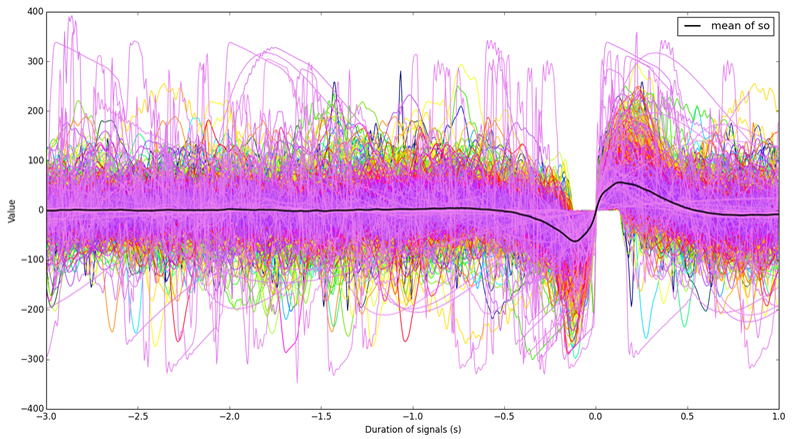
\includegraphics[width = 0.8\linewidth]{graphics/EEG_oscillation.png}\\
        		\vspace{5pt}
        		\alert{Section 4}
        	\end{column}
        	\begin{column}{.5\linewidth}
        		Image Denoising\\
        		\vspace{5pt}
        		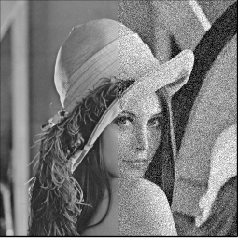
\includegraphics[width = 0.6\linewidth]{graphics/lena_pic.jpg}\\
        		\vspace{5pt}
        		\alert{Section 5}
        	\end{column}
        \end{columns}
  \end{frame}

  \begin{frame}\frametitle{Introduction: ML and Optimization I}
    \alert{Training} a Machine Learning model means finding optimal parameters $\omega$:

    $$ \omega^* = \argmin_{\omega} F(\omega, X, z)$$
    
    \begin{itemize}
      \item \alert{$F$}: Loss function
      \item \alert{$X$}: The training data
      \item \alert{$z$}: Training labels
    \end{itemize}   
  \end{frame}

  \begin{frame}\frametitle{Introduction: ML and Optimization II}
    After we have found $\omega^*$, we can do \alert{Prediction} on new data points:

    $$ \hat {z_i} := h(\omega^*, x_i)$$
    
    \begin{itemize}
      \item \alert{$x_i$}: new data point with \emph{unknown} label \alert{$z_i$}
      \item \alert{$h$}: hypothesis function of the ML model
    \end{itemize}   
  \end{frame}

  \begin{frame}
    \frametitle{Introduction: Challenges in Machine Learning}
      \begin{itemize}
        \item Massive amounts of training data 
        \item Construction of very large models
        \item Handling high memory/computational demands
      \end{itemize}
      \vspace{35pt}
    \centering \huge{\alert{Stochastic Methods}}
  \end{frame}
  
  \begin{frame}{Introduction: Stochastic Framework}
    $$ F(\omega) := \mathbb{E}\left[f(\omega, \xi)\right] \uncover<3->{= \frac{1}{N}\sum_{i=1}^N f(\omega, x_i, z_i)}$$
    \begin{itemize}
      \item<2-> \alert{$\xi$}: Random variable; takes the form of an input-output-pair $(x_i, z_i)$
      \item<3-> \alert{$f$}: Partial loss function corresponding to a single data point.
      \item<4-> Example loss function: $f(\omega, x_i, z_i) = |z_i - \omega^Tx_i|$ (Linear Regression)
    \end{itemize}
  \end{frame}

  \begin{frame}{Introduction: Stochastic Methods}
    \begin{columns}[T]
      \begin{column}{.5\textwidth}
        \centering \alert{Gradient Method}
        $$\min F(\omega) $$
        \phantom{0}
        
        $$\omega^{(k+1)}:= \omega^{k}-\alpha_k \nabla F(\omega^{k})$$\\
        \phantom{zeile}
        
      \end{column}\hfill
      \begin{column}{.5\textwidth}
        \centering \alert{Stochastic Gradient Descent (SGD)}
        $$\min \mathbb E \left [f(\omega, \xi)\right]$$
        \uncover<2>{
          $$\omega^{k+1}:= \omega^{k}-\alpha_k \alert{\nabla \hat F(\omega^{k})} $$
          with
          $$\alert{\nabla \hat F(\omega^{k})} := \frac{1}{b}\sum_{i\in \mathcal S_k}\nabla f(\omega^k, x_i, z_i)$$
          where $\mathcal S_k \subset [N], \quad b:=|\mathcal S_k| \ll N$\\\alert{"Mini Batch"}
        }
      \end{column}
    \end{columns}
  \end{frame}

\section{SQN: A Stochastic Quasi-Newton Method}

 
  \begin{frame}{Stochastic Newton Method}

  	\begin{columns}[T]
  		\begin{column}{.5\textwidth}
  			\centering \alert{Stochastic Gradient Descent}
  			$$\min \mathbb E \left [f(\omega, \xi)\right]$$
  				$$\omega^{k+1}:= \omega^{k}-\alpha_k \nabla \hat F(\omega^{k}) $$
  				
  				$$\nabla \hat F(\omega^{k}) := \frac{1}{b}\sum_{i\in \mathcal S_k}\nabla f(\omega^k, x_i, z_i)$$

  		\end{column}\hfill
  		\begin{column}{.5\textwidth}
  			\centering \alert{Stochastic Newton Method}
  			$$\min \mathbb E \left [f(\omega, \xi)\right]$$
  			\uncover<2>{
  				$$\omega^{k+1}:= \omega^{k}-\alpha_k \alert{\nabla^2 \hat F(\omega^{k})^{-1}} {\nabla \hat F(\omega^{k})} $$
  				with
  				$$\alert{\nabla^2 \hat F(\omega^{k})} := \frac{1}{b_H}\sum_{i\in \mathcal S_{H,\alert{t}}}\nabla^2 f(\omega^{\alert{t}}, x_i, z_i)$$
          where $\mathcal S_{H,\alert{t}} \subset [N], \quad b_H:=|\mathcal S_{H,\alert{t}}| \ll N$,\\
          $\alert{(t)}$ subsequence of $(k)$
          }
  		\end{column}
  	\end{columns}
  \end{frame}

  \begin{frame}\frametitle{Stochastic Quasi-Newton Method (SQN)}
      \begin{itemize}
        \item \alert{Stochastically} use second-order information
        \item Approximate $\nabla ^2 \hat F(\omega^{k})$ by BFGS matrix $H_t$
        \item $t$ running on slower time-scale than $k$. 
        \item $H_t$ update in $\mathcal O(n)$ time and constant memory, using several tricks
      \end{itemize}
  \end{frame}

  \begin{frame}
    \frametitle{SQN: Performance I}

      \begin{columns}[T]
      \begin{column}{.5\textwidth}
        \resizebox{\linewidth}{!}{% This file was created by matplotlib v0.1.0.
% Copyright (c) 2010--2014, Nico Schlömer <nico.schloemer@gmail.com>
% All rights reserved.
% 
% The lastest updates can be retrieved from
% 
% https://github.com/nschloe/matplotlib2tikz
% 
% where you can also submit bug reports and leavecomments.
% 
\begin{tikzpicture}

\definecolor{color1}{rgb}{1,0.728139904610493,0}
\definecolor{color0}{rgb}{1,0,0.16}
\definecolor{color3}{rgb}{0,1,0.548176259751213}
\definecolor{color2}{rgb}{0.36036036036036,1,0}
\definecolor{color5}{rgb}{0.354859335038363,0,1}
\definecolor{color4}{rgb}{0,0.56159420289855,1}
\definecolor{color6}{rgb}{1,0,0.75}

\begin{axis}[
title={EEG: Sample Objective vs. Iterations},
xlabel={Iterations},
ylabel={$F_{S_k}(\omega^k)$},
xmin=0, xmax=200,
ymin=0.8, ymax=100,
ymode=log,
axis on top
]
\addplot [color0, dashed]
coordinates {
(0,79.0395277038001)
(1,71.656802715)
(1.99999999999999,57.2088643197)
(3,54.0859214048)
(4,48.4329980926)
(5,45.9896987415)
(5.99999999999999,39.6427124165)
(7,39.1160717119)
(8,33.5967875488)
(8.99999999999999,31.4090047632)
(10,30.4467400339)
(11,26.9244848041)
(12,28.729948616)
(13,27.300592885)
(14,24.8019499379)
(15,23.0659266308)
(16,22.2785131853)
(17,20.9370524433)
(18,19.6796621939)
(19,20.6142355004)
(20,23.7980394087)
(21,18.9382364564)
(22,22.9292653548)
(23,22.8607098199)
(24,20.4630749567)
(25,24.8523685932)
(26,24.0522449193)
(27,20.2649498017)
(28,20.8349264756)
(29,22.5004323131)
(30,17.4659060115)
(31,14.875970104)
(32,16.3188693866)
(33,17.6760948707)
(34,15.1257468437)
(35,16.7907311103)
(36,14.4970054579)
(37,15.5408352527)
(38,11.8928123182)
(39,17.473859118)
(40,16.6670595516)
(41,17.3692768959)
(42,15.4024712072)
(43,15.6653245483)
(44,18.7499125723)
(45,15.5451484755)
(46,17.2901069358)
(47,18.8885565266)
(48,20.193850162)
(49,18.8113648621)
(50,16.3790920442)
(51,19.0291634227)
(52,16.1105300083)
(53,17.6046852134)
(54,13.4469661072)
(55,15.687254446)
(56,13.7687201819)
(57,13.5380248903)
(58,16.2565260155)
(59,16.8390100165)
(60,14.8931541718)
(61,14.4763756076)
(62,14.4421662936)
(63,15.594649077)
(64,11.5832518212)
(65,15.1356912094)
(66,11.691773837)
(67,16.1037206044)
(68,13.6780255639)
(69,10.3866920851)
(70,12.9568987123)
(71,10.7826169744)
(72,13.1718456817)
(73,14.7380910294)
(74,17.05068962)
(75,12.3612466376)
(76,10.9339959304)
(77,10.846600434)
(78,10.1580378629)
(79,11.8329911894)
(80,14.4714123232)
(81,10.0056540191)
(82,9.34458971235)
(83,10.9932479488)
(84,9.93589442385)
(85,11.5679498036)
(86,8.7387604647)
(87,9.48104172491)
(88,9.94672203629)
(89,8.07586263982)
(90,10.8540522581)
(91,11.0811664217)
(92,12.6152548631)
(93,9.99694089572001)
(94,11.0622966781)
(95,9.6548830997)
(96,10.0185245722)
(97,10.6762123895)
(98,11.1676393887)
(99,9.90977290666001)
(100,7.17433932649)
(101,5.75079869679)
(102,6.2652006362)
(103,7.69321596697)
(104,9.28684121714001)
(105,11.5580682599)
(106,10.1711712001)
(107,12.8001778838)
(108,12.6494529662)
(109,10.1951851509)
(110,9.56142792305)
(111,9.15387074981)
(112,8.30423788170001)
(113,9.46082249272)
(114,8.69145512189001)
(115,9.36131809607001)
(116,8.96048771228)
(117,7.64247656412)
(118,5.81563704453)
(119,8.10127003759)
(120,8.36983406295001)
(121,9.08582278373)
(122,7.7557318775)
(123,10.4954247046)
(124,9.48109606927)
(125,9.05141953131)
(126,7.97006074530001)
(127,10.2373826223)
(128,11.9095210124)
(129,12.0521715129)
(130,14.1117360836)
(131,11.2039492754)
(132,13.3753125988)
(133,14.0193127535)
(134,10.5939782721)
(135,11.4660695015)
(136,12.8114158221)
(137,11.2570596365)
(138,13.9796865227)
(139,15.1819410836)
(140,15.752132436)
(141,13.4665480371)
(142,13.3058032288)
(143,15.6428714038)
(144,13.5835502199)
(145,11.1403344661)
(146,13.8321495692)
(147,15.6129372538)
(148,16.5426655116)
(149,17.1088546102)
(150,12.2843844792)
(151,12.9388141152)
(152,10.6732913)
(153,12.9899076141)
(154,13.3563185094)
(155,14.0057744954)
(156,13.2919533085)
(157,12.4768264854)
(158,10.5956200732)
(159,9.86814319778001)
(160,10.2325922162)
(161,11.2401520936)
(162,11.3452659073)
(163,14.2691415964)
(164,11.2991814749)
(165,9.81844220354001)
(166,9.88126493934)
(167,10.535767431)
(168,10.4613901525)
(169,11.4399876364)
(170,10.6323697723)
(171,8.96436380315)
(172,8.92203480667001)
(173,7.40887099586)
(174,8.01111984875)
(175,8.60852297356)
(176,8.71319062117)
(177,8.31559178543001)
(178,8.96290678716)
(179,9.97009603658)
(180,10.4368088466)
(181,7.54612922042)
(182,9.94564211089)
(183,11.0177233484)
(184,8.18973299366)
(185,10.2701884798)
(186,8.19185184522)
(187,8.08407981202)
(188,8.56081397047)
(189,11.063832058)
(190,10.5273179747)
(191,10.6678088708)
(192,8.79375054503)
(193,11.5887553744)
(194,13.683726671)
(195,12.0621961866)
(196,12.4895163178)
(197,11.4886931628)
(198,13.7241381187)
(199,16.0062841825)
(200,13.4328508646)
(201,14.7664149504)
(202,11.8338014499)
(203,12.6935305402)
(204,14.5630181458)
(205,12.0586979218)
(206,14.8061108443)
(207,10.7195894039)
(208,11.4833176182)
(209,13.2299405504)
(210,13.1355307117)
(211,14.4231840584)
(212,16.538079362)
(213,17.0419870416)
(214,15.9909430057)
(215,18.0441760078)
(216,15.0493456151)
(217,12.4066383103)
(218,11.31976687)
(219,12.2392589045)
(220,11.2947724126)
(221,12.6670925742)
(222,12.2725393637)
(223,12.74926528)
(224,14.0868070597)
(225,12.9932522606)
(226,11.1735023234)
(227,12.3847453738)
(228,13.7971278391)
(229,13.1090245146)
(230,10.9037741558)
(231,13.5403386859)
(232,15.060839202)
(233,13.058474328)
(234,12.7009535132)
(235,14.4086263717)
(236,12.5440785233)
(237,11.8906318109)
(238,12.5108682846)
(239,10.8123214851)
(240,13.367364829)
(241,16.5441379898)
(242,19.1698052096)
(243,15.3048952195)
(244,15.3810067554)
(245,14.6358393147)
(246,14.1799008749)
(247,15.7953296627)
(248,14.3735759744)
(249,13.9814459771)
(250,13.7215248521)
(251,13.8793953746)
(252,15.5926480646)
(253,11.4232905537)
(254,12.6289419683)
(255,15.4840382947)
(256,15.0854207155)
(257,16.3063794111)
(258,12.3343756354)
(259,13.8666351011)
(260,11.1292895029)
(261,12.8022407041)
(262,11.8756548618)
(263,13.4254127628)
(264,13.3442819805)
(265,14.1707670568)
(266,15.781747592)
(267,13.556177709)
(268,13.1955444988)
(269,15.6953680772)
(270,12.908394941)
(271,8.52715093544)
(272,11.2569103158)
(273,13.0148745262)
(274,13.4353101122)
(275,15.2480814165)
(276,15.0167505016)
(277,13.576852166)
(278,12.1493334144)
(279,11.3393062125)
(280,11.4687464191)
(281,9.78482890895)
(282,11.3534518741)
(283,12.6818838625)
(284,12.6258597925)
(285,14.1623700048)
(286,16.8884123082)
(287,15.0343703263)
(288,14.6255346985)
(289,15.3162647697)
(290,17.676211092)
(291,17.5507082762)
(292,17.1519398059)
(293,18.7413915475)
(294,12.4080082804)
(295,15.2094287017)
(296,15.4007681382)
(297,15.1794109577)
(298,13.9675644874)
(299,14.6620707109)
(300,18.3883594308)
(301,14.8194078369)
(302,12.780918189)
(303,14.0879753465)
(304,13.973558444)
(305,12.3907075005)
(306,13.0503443619)
(307,11.685191262)
(308,11.8071349235)
(309,12.6169083183)
(310,11.568530595)
(311,12.1671817955)
(312,11.3916202174)
(313,10.5834545684)
(314,11.2908068398)
(315,9.71154389246001)
(316,8.22677272481001)
(317,6.20438928751)
(318,5.89556052586)
(319,8.26169168133)
(320,7.32196868383)
(321,8.25079550001)
(322,8.55562577069)
(323,5.11852061598)
(324,8.23540254711)
(325,7.41680467912)
(326,5.6395681661)
(327,6.04267757158)
(328,8.8485808313)
(329,11.0055418656)
(330,11.2942251139)
(331,11.5369000316)
(332,8.75907954694001)
(333,8.66488565316)
(334,10.7946966063)
(335,7.6920821934)
(336,7.80265557815)
(337,7.13622054265)
(338,5.86516483526)
(339,9.29406106763)
(340,12.7193993546)
(341,10.230665359)
(342,9.88100211899)
(343,10.5600681033)
(344,11.5938872876)
(345,9.45918469444)
(346,8.89996652620001)
(347,7.33650541508)
(348,8.01011606551)
(349,10.2113466044)
(350,13.3785566218)
(351,12.085788743)
(352,13.9569722301)
(353,13.4801889209)
(354,14.9156639573)
(355,16.1184707652)
(356,12.9346230029)
(357,13.6646812946)
(358,15.3022112707)
(359,13.2506805085)
(360,11.9277787552)
(361,12.7395484825)
(362,14.4778861453)
(363,15.9884753618)
(364,12.2759849253)
(365,14.4812461928)
(366,12.157906576)
(367,13.4146779802)
(368,13.5218393968)
(369,14.3754268743)
(370,17.7930776088)
(371,13.8989465363)
(372,14.8674489914)
(373,15.0527654278)
(374,12.6577729934)
(375,11.5099160769)
(376,11.0334324858)
(377,10.4646998314)
(378,16.5969445522)
(379,14.4366416862)
(380,13.6981165526)
(381,13.4442243349)
(382,12.4734202699)
(383,15.5250059902)
(384,14.2328666677)
(385,13.4843546767)
(386,13.6528421098)
(387,13.7471476064)
(388,18.0572129287)
(389,13.2875922756)
(390,15.3356144509)
(391,15.8430861158)
(392,13.2642682971)
(393,16.1128014165)
(394,15.466299842)
(395,15.7846843298)
(396,14.0359567398)
(397,14.2669115501)
(398,15.1829699856)
(399,13.6408357254)
(400,14.8418178526)
(401,11.2520555763)
(402,11.6765115731)
(403,9.80017658756)
(404,9.60818086403001)
(405,9.90433532637)
(406,11.7946162447)
(407,11.1894859047)
(408,13.2191508026)
(409,13.7584523727)
(410,14.4607548897)
(411,14.0356752109)
(412,12.0071366005)
(413,11.7816435259)
(414,13.1208349862)
(415,13.0580048441)
(416,13.6152338761)
(417,13.7287340992)
(418,14.5706315581)
(419,12.9955672822)
(420,11.9129523456)
(421,12.7130607686)
(422,18.3343427215)
(423,11.1770422314)
(424,12.5574229502)
(425,11.4135468946)
(426,9.82853350105)
(427,11.5489686606)
(428,12.2981406088)
(429,14.4284655953)
(430,11.8250351263)
(431,15.6398218465)
(432,12.7807600797)
(433,14.3041687197)
(434,14.4414312861)
(435,12.124645034)
(436,10.9399369936)
(437,10.1927598271)
(438,10.2515551158)
(439,7.99973507008)
(440,12.3001089277)
(441,16.5565681995)
(442,11.877014386)
(443,13.2462486518)
(444,11.9008390184)
(445,12.1340762365)
(446,9.36615583265)
(447,10.3534788978)
(448,8.42858394071)
(449,9.88798145091)
(450,10.5614458839)
(451,13.4138665158)
(452,13.3012645461)
(453,15.2275959493)
(454,14.739711569)
(455,14.9242305641)
(456,15.1959789575)
(457,13.3585150867)
(458,10.5306726349)
(459,13.828729563)
(460,16.672869924)
(461,14.9819698572)
(462,15.0469396841)
(463,15.7507779077)
(464,17.1061830809)
(465,16.932764534)
(466,13.9451218876)
(467,16.2230043588)
(468,14.8692854199)
(469,13.4021169362)
(470,16.2136251507)
(471,16.3388288656)
(472,13.9924222228)
(473,12.0417736663)
(474,14.4435242315)
(475,16.5258135242)
(476,15.2945660558)
(477,14.9167482515)
(478,15.587603536)
(479,14.6666956331)
(480,11.8559420081)
(481,15.3684553595)
(482,14.2159494908)
(483,14.9156521721)
(484,14.6706813556)
(485,16.4456628034)
(486,17.7333179566)
(487,15.1451296983)
(488,15.4156997849)
(489,12.5042289623)
(490,11.8554395505)
(491,9.34202614176)
(492,11.0387952282)
(493,14.7686267114)
(494,17.2128453298)
(495,15.9188867623)
(496,14.3004458348)
(497,13.4688124421)
(498,11.5974729186)
(499,12.897437004)
(500,13.2506435864)
(501,12.4510119715)
(502,10.5439169975)
(503,11.8426783767)
(504,15.309420045)
(505,13.7355377128)
(506,10.0280474669)
(507,10.0393209307)
(508,11.4824811925)
(509,14.2255414123)
(510,12.4758819333)
(511,10.1374768618)
(512,12.2164929331)
(513,11.802075867)
(514,14.3328746374)
(515,11.9702550889)
(516,14.0709558311)
(517,11.8832661583)
(518,10.8542636122)
(519,13.2696791134)
(520,12.4831661502)
(521,11.7689176355)
(522,8.84481265291001)
(523,11.304341752)
(524,10.9057568721)
(525,14.1102263524)
(526,13.1172891892)
(527,14.6971851018)
(528,13.7706661355)
(529,14.9456907947)
(530,14.4896345669)
(531,14.9512702714)
(532,14.3785947067)
(533,11.0252862959)
(534,11.4978416022)
(535,13.8585475706)
(536,15.2706739313)
(537,13.4328565789)
(538,14.0477236753)
(539,11.3603471995)
(540,11.145069475)
(541,13.4492714689)
(542,13.022954501)
(543,12.7940881901)
(544,12.5601073222)
(545,13.3928641354)
(546,12.7736115743)
(547,14.3356859105)
(548,12.8866599819)
(549,12.7319676072)
(550,12.4078272332)
(551,11.9354143034)
(552,11.5893407491)
(553,8.69920588316)
(554,10.9021871805)
(555,9.71909270488)
(556,10.2849053086)
(557,7.85791844499)
(558,9.40164281832)
(559,8.96900994054)
(560,10.6950199574)
(561,8.78661875606)
(562,10.7948852171)
(563,11.6485744211)
(564,10.5826766258)
(565,9.69343347006)
(566,13.1025895738)
(567,16.7130686158)
(568,16.2064992842)
(569,12.0586876613)
(570,13.0445489775)
(571,11.0525452376)
(572,10.8756650636)
(573,10.1343706775)
(574,14.495501603)
(575,9.84304500433)
(576,10.0660857427)
(577,9.57604243353)
(578,9.71691037672)
(579,10.2696767736)
(580,12.0921766882)
(581,12.8712928367)
(582,11.9322932728)
(583,11.3276703207)
(584,10.1906602431)
(585,10.3347350299)
(586,13.411938194)
(587,13.9201778342)
(588,13.0811065782)
(589,11.4726143144)
(590,12.7872519783)
(591,15.5296337757)
(592,15.2221137369)
(593,13.9878793091)
(594,13.6215488005)
(595,11.6442368904)
(596,13.9895046459)
(597,12.2522666179)
(598,12.2649781853)
(599,11.3022220307)
(600,9.21187742603001)
(601,10.3018966553)
(602,10.7238628493)
(603,7.4680402919)
(604,5.95396372934)
(605,7.96012441125)
(606,9.07001626108)
(607,9.58282900787)
(608,8.69566688575)
(609,9.79190897621)
(610,8.8780307639)
(611,5.47529018407)
(612,5.99377709188)
(613,5.48973599686)
(614,7.67599606572)
(615,9.88659317619)
(616,11.2211467914)
(617,12.9175495185)
(618,11.9589255819)
(619,12.9134615183)
(620,14.3195829108)
(621,12.2511281527)
(622,11.9759936437)
(623,11.106214929)
(624,9.64407014844)
(625,9.5418454311)
(626,11.1434390333)
(627,9.24418753793999)
(628,8.87572418757999)
(629,9.44338169249)
(630,7.57416830773)
(631,8.2054184376)
(632,7.80160531892001)
(633,8.55596576732)
(634,8.10907619859)
(635,12.7621371648)
(636,12.4504326338)
(637,11.501350933)
(638,13.6807297641)
(639,11.3875443875)
(640,10.1719192631)
(641,10.6641186976)
(642,12.3380828561)
(643,11.0759927326)
(644,8.36974133703)
(645,11.3135467016)
(646,9.04172170112)
(647,10.8175423953)
(648,10.552121605)
(649,13.4846437206)
(650,10.978287513)
(651,10.8677444642)
(652,14.1912065066)
(653,12.590309266)
(654,13.8000574661)
(655,13.8268125676)
(656,15.1500761781)
(657,13.5159293966)
(658,12.7299571237)
(659,11.5991103481)
(660,13.8504582167)
(661,13.7333742278)
(662,14.3074107208)
(663,13.9658880502)
(664,12.3464003331)
(665,13.6456350371)
(666,12.7635129678)
(667,12.2257470819)
(668,14.6286451395)
(669,10.8551589383)
(670,15.6856904738)
(671,17.4514672537)
(672,11.3142910995)
(673,14.0315704186)
(674,13.6945880526)
(675,15.945260415)
(676,13.7183526239)
(677,13.336373482)
(678,11.5151825673)
(679,12.2435998435)
(680,12.7258670042)
(681,9.83121909646)
(682,10.5407198603)
(683,14.3506621905)
(684,16.8880846486)
(685,14.1715783517)
(686,14.1868540795)
(687,11.7101814169)
(688,12.2707721525)
(689,13.5340322707)
(690,12.5087448267)
(691,13.26007772)
(692,15.4185768432)
(693,13.7094421573)
(694,13.7755787293)
(695,16.8224765052)
(696,15.5947365532)
(697,13.8892467568)
(698,13.9292890874)
(699,15.2609996678)
(700,15.4133595242)
(701,13.9871260834)
(702,15.4467726985)
(703,13.9393788611)
(704,11.688246386)
(705,9.79988531051)
(706,9.87667572761001)
(707,10.9189069786)
(708,12.4119898977)
(709,9.47765244094999)
(710,10.8679271018)
(711,10.0705659583)
(712,12.186689849)
(713,11.7506114229)
(714,14.1327563989)
(715,13.3395985834)
(716,13.7839544265)
(717,13.1973506012)
(718,7.95763208437)
(719,9.61442531297)
(720,14.16758703)
(721,11.0464026291)
(722,14.429482096)
(723,12.8537555407)
(724,13.9476797285)
(725,12.9850349344)
(726,10.2058256472)
(727,16.0358657542)
(728,15.7886094619)
(729,14.3112359452)
(730,16.8973318441)
(731,15.3248330432)
(732,14.4663661141)
(733,12.4140559625)
(734,13.6464190406)
(735,15.5931593493)
(736,15.677938386)
(737,15.8517179995)
(738,14.5517044853)
(739,15.1110090967)
(740,10.2298432465)
(741,12.4216743224)
(742,14.0240955034)
(743,11.3235532849)
(744,18.0373963434)
(745,15.7820205084)
(746,16.803249819)
(747,11.1117869475)
(748,12.6794807909)
(749,16.0157121572)
(750,13.9761438099)
(751,15.3070821226)
(752,14.8060077441)
(753,17.6817351672)
(754,14.4046211348)
(755,13.4769600753)
(756,14.3167684172)
(757,13.9527502436)
(758,16.2265017555)
(759,12.102992491)
(760,12.6063826983)
(761,13.3126833573)
(762,11.9801528028)
(763,14.2992661011)
(764,14.7719191555)
(765,14.4504286374)
(766,14.3968169515)
(767,13.4828995154)
(768,12.7849205905)
(769,14.2349895663)
(770,14.0654811621)
(771,13.6866823143)
(772,12.6726447703)
(773,12.4646333447)
(774,13.0416955042)
(775,12.673946329)
(776,14.1283314875)
(777,11.9967580337)
(778,13.0000163658)
(779,12.9692108)
(780,15.4855415074)
(781,15.6060693821)
(782,14.6665883078)
(783,12.9578383607)
(784,10.2798961096)
(785,12.9116042444)
(786,13.5614673376)
(787,11.2511628653)
(788,11.8894316925)
(789,10.2567030178)
(790,10.6449703219)
(791,8.06807975379)
(792,9.5802397765)
(793,12.3202491141)
(794,11.3476024663)
(795,13.3980899451)
(796,11.373537303)
(797,13.8853887405)
(798,12.1828225059)
(799,13.8536814198)
(800,10.6319695859)
(801,14.2102157567)
(802,12.7553706392)
(803,13.5681722024)
(804,15.3964863501)
(805,14.7040755073)
(806,16.2431958664)
(807,12.9595488333)
(808,12.9665642072)
(809,15.6137777373)
(810,14.2447168668)
(811,13.2191308676)
(812,10.6457256529)
(813,10.5279398807)
(814,13.0502188632)
(815,9.87090853608)
(816,11.4582417015)
(817,12.2443131806)
(818,13.346406684)
(819,15.5224341424)
(820,14.7471554911)
(821,13.237504659)
(822,14.9279396376)
(823,14.9517188741)
(824,13.429750716)
(825,13.2283794941)
(826,12.7487835451)
(827,13.7393162914)
(828,14.7992732573)
(829,13.931005566)
(830,14.3268571996)
(831,14.4155495118)
(832,15.0165787691)
(833,11.7627665643)
(834,9.82325511282999)
(835,12.0076460172)
(836,11.7460164467)
(837,13.7443141994)
(838,17.712751136)
(839,14.4170244628)
(840,13.8106922483)
(841,13.0732359711)
(842,15.4459773406)
(843,17.9832242193)
(844,13.0811809982)
(845,12.1185793599)
(846,12.6470682961)
(847,11.1735007265)
(848,10.8845788969)
(849,13.6917123398)
(850,11.6147671915)
(851,14.1960224372)
(852,13.8151049904)
(853,12.0938345713)
(854,10.4708124072)
(855,13.3404458636)
(856,13.3973839611)
(857,13.4152961365)
(858,11.022946569)
(859,10.6221662912)
(860,10.7658597965)
(861,11.7002994287)
(862,13.1129709642)
(863,11.9764671337)
(864,12.4239326972)
(865,12.9547956198)
(866,11.61392163)
(867,11.15948049)
(868,11.2100225358)
(869,10.3426049124)
(870,12.1874173887)
(871,12.2729104746)
(872,12.5690611097)
(873,13.3073320005)
(874,14.4804299488)
(875,11.5871708169)
(876,9.26183493081)
(877,12.2135029131)
(878,11.5905373149)
(879,10.8521196846)
(880,11.9314536493)
(881,9.8388221883)
(882,11.8333449578)
(883,10.824512376)
(884,10.862023832)
(885,6.03976035849)
(886,10.7128865819)
(887,11.4454366177)
(888,11.3140714538)
(889,11.0554709458)
(890,10.788429186)
(891,10.261131257)
(892,11.965318602)
(893,10.6737666496)
(894,9.48373515470001)
(895,11.3624050947)
(896,11.5521007319)
(897,12.3240550458)
(898,8.73804328807)
(899,10.2933711776)
(900,12.422710523)
(901,12.9305454079)
(902,9.41316981451)
(903,12.0506622492)
(904,12.7652772691)
(905,14.635021053)
(906,14.834719386)
(907,10.2554713326)
(908,13.4862441534)
(909,13.271013813)
(910,14.053577731)
(911,12.5053826326)
(912,13.4126170345)
(913,15.8253322935)
(914,15.8253150175)
(915,15.6282985164)
(916,14.9036894025)
(917,13.5644255733)
(918,14.1464080302)
(919,12.1318970219)
(920,11.2987693927)
(921,9.9742374018)
(922,13.2962991581)
(923,10.891319638)
(924,12.4803454133)
(925,11.0658501695)
(926,10.4869054154)
(927,8.89289440461001)
(928,11.5216016999)
(929,7.22936745867)
(930,13.476522452)
(931,12.7192410827)
(932,13.5548976559)
(933,11.840716888)
(934,14.9124246278)
(935,12.3569486078)
(936,12.2720461558)
(937,11.0497553092)
(938,13.4670982051)
(939,14.782397294)
(940,11.9288407221)
(941,11.7812815879)
(942,9.25582254008999)
(943,10.4284839091)
(944,10.6874637477)
(945,12.881041547)
(946,12.1406188248)
(947,13.0946857085)
(948,11.4404927008)
(949,12.9521731995)
(950,12.7515309666)
(951,9.78930394639)
(952,10.033152521)
(953,7.45665122917)
(954,10.7538412262)
(955,9.38580858131001)
(956,7.66803377824001)
(957,9.34514151725999)
(958,7.51733170529)
(959,7.23239351196)
(960,7.66842909925)
(961,8.70823800345)
(962,10.0689793277)
(963,9.83257169337)
(964,10.6371110692)
(965,11.2377063413)
(966,9.2034423694)
(967,8.14942359171001)
(968,8.40066945042)
(969,11.9047123098)
(970,9.9416197573)
(971,8.87631444004)
(972,10.721305259)
(973,8.81841897954)
(974,12.5856807386)
(975,13.2194052299)
(976,12.4220493052)
(977,11.3147709869)
(978,8.01176125996)
(979,7.67663739599)
(980,10.9599845809)
(981,8.43460966496)
(982,7.36575087913)
(983,8.58582723361001)
(984,10.9718029928)
(985,12.340810317)
(986,10.7797094738)
(987,12.6174115242)
(988,13.6625235397)
(989,11.817456314)
(990,14.2422619879)
(991,13.947986948)
(992,13.4653936348)
(993,11.9449698334)
(994,14.6795469394)
(995,12.7250138966)
(996,11.8474319372)
(997,10.0354110035)
(998,10.4681008411)
(999,11.649410334)
(1000,9.70826734078)
(1001,10.8462252968)
(1002,11.7550946266)
(1003,12.8751532821)
(1004,13.480146259)
(1005,13.7347127466)
(1006,15.6384628831)
(1007,13.7843044393)
(1008,12.1478174337)
(1009,14.2400787127)
(1010,12.1858003918)
(1011,13.4876885405)
(1012,12.516123845)
(1013,10.790383208)
(1014,14.3905015447)
(1015,12.8066873924)
(1016,12.617623299)
(1017,12.7823941904)
(1018,13.3106502449)
(1019,15.051363749)
(1020,15.0768152936)
(1021,15.3333106894)
(1022,13.8745491721)
(1023,16.0372504007)
(1024,15.2570579609)
(1025,15.3001488077)
(1026,11.5260298427)
(1027,10.2653615767)
(1028,14.377054992)
(1029,15.577022592)
(1030,12.8001334714)
(1031,14.6966187477)
(1032,13.9835717369)
(1033,11.2283805935)
(1034,11.2831749876)
(1035,13.1977066107)
(1036,13.8398444924)
(1037,11.7263177338)
(1038,9.14749894544)
(1039,10.7102653367)
(1040,12.0766975615)
(1041,15.3146078141)
(1042,12.7728967139)
(1043,15.5376279259)
(1044,14.6286917326)
(1045,12.0616503114)
(1046,11.6448863456)
(1047,11.2412741802)
(1048,11.4710948466)
(1049,11.3248049965)
(1050,8.64806435671)
(1051,10.147007839)
(1052,8.94213980703)
(1053,8.82862087874)
(1054,7.3381332981)
(1055,7.99174340481)
(1056,9.07405427482001)
(1057,10.1969010122)
(1058,10.3737798323)
(1059,10.8983393327)
(1060,10.5922113616)
(1061,14.3348865907)
(1062,11.9505322321)
(1063,11.8476410025)
(1064,16.594014587)
(1065,18.4421309559)
(1066,16.4164412944)
(1067,14.2960786849)
(1068,13.3575568301)
(1069,14.1569876729)
(1070,14.8923491135)
(1071,16.735102925)
(1072,14.8719465893)
(1073,12.0347207333)
(1074,12.474814439)
(1075,12.9090574272)
(1076,16.4608247963)
(1077,14.5951472404)
(1078,13.5059305016)
(1079,13.8828114185)
(1080,10.8548394111)
(1081,12.6179883053)
(1082,11.2285748589)
(1083,12.6416880504)
(1084,10.9556647459)
(1085,9.2688219291)
(1086,8.20959644998999)
(1087,8.05715440142999)
(1088,9.51170043148)
(1089,8.85415308251)
(1090,11.2548074764)
(1091,13.7922804046)
(1092,12.0329125979)
(1093,13.0463697001)
(1094,15.4290279148)
(1095,16.1331818915)
(1096,12.8681044767)
(1097,13.6783750856)
(1098,13.1199152209)
(1099,10.3215485943)
(1100,12.7626637675)
(1101,11.0730110837)
(1102,13.1496063316)
(1103,12.8433381993)
(1104,11.868894044)
(1105,10.8779032626)
(1106,12.7815685446)
(1107,10.8517026635)
(1108,13.5031836046)
(1109,12.1978188216)
(1110,11.8155086347)
(1111,9.29877668012)
(1112,9.72706753805)
(1113,11.2265820342)
(1114,8.09618796437)
(1115,9.8786834376)
(1116,7.55104414609)
(1117,8.31531440971)
(1118,8.94501670742001)
(1119,10.3039187181)
(1120,6.51854702893)
(1121,8.72987886139)
(1122,6.82512269882)
(1123,11.7236592679)
(1124,11.982935114)
(1125,9.36354978311)
(1126,7.24685823333999)
(1127,9.31283584062)
(1128,9.66997889799)
(1129,13.002974662)
(1130,14.1309635415)
(1131,13.0450714747)
(1132,12.5620750454)
(1133,11.9859657333)
(1134,9.23991190685)
(1135,12.19109941)
(1136,11.7573207498)
(1137,11.8699305184)
(1138,15.7851483315)
(1139,14.6529226444)
(1140,12.5408813633)
(1141,11.4442286759)
(1142,10.7414808671)
(1143,14.3839989351)
(1144,14.4828597587)
(1145,15.199089358)
(1146,16.8761832599)
(1147,15.8570584819)
(1148,12.4320038565)
(1149,12.1901391382)
(1150,13.6894962672)
(1151,13.9355824178)
(1152,10.7989364984)
(1153,11.7335202278)
(1154,11.5954401728)
(1155,11.624250143)
(1156,11.5280350955)
(1157,8.82712080834)
(1158,9.70244651257)
(1159,8.69673178071)
(1160,7.69390963411001)
(1161,5.49437897807)
(1162,8.62493967904001)
(1163,10.3784286866)
(1164,8.23365544453)
(1165,9.21601851374)
(1166,8.98671654517)
(1167,7.19869559034)
(1168,7.86030849119)
(1169,10.1672659051)
(1170,8.36081416254)
(1171,9.53892574505)
(1172,10.747328761)
(1173,8.93426525588)
(1174,5.8489590938)
(1175,8.12887209041001)
(1176,7.71374586059)
(1177,6.76814573646)
(1178,7.8563467981)
(1179,7.45873666161)
(1180,8.29326630286001)
(1181,9.42602461561)
(1182,9.24176326673001)
(1183,10.2786381577)
(1184,8.61016843483)
(1185,6.33778730025)
(1186,6.45024991085001)
(1187,8.07834311064)
(1188,5.56679559588001)
(1189,8.89085496222)
(1190,11.0806041278)
(1191,10.4713818597)
(1192,12.5732978063)
(1193,16.3414808038)
(1194,12.322909669)
(1195,11.4602440921)
(1196,10.9609600021)
(1197,9.96251016393)
(1198,10.3495067953)
(1199,10.8397213245)
(1200,9.03553934813)
(1201,8.54413332323)
(1202,9.22954258657)
(1203,10.0842430662)
(1204,9.51765715554)
(1205,10.101762415)
(1206,9.65476808088)
(1207,11.1727834551)
(1208,13.6200333319)
(1209,12.5916501787)
(1210,14.8960931481)
(1211,14.5877692882)
(1212,15.2807568751)
(1213,16.5691158855)
(1214,20.0780992936)
(1215,16.9515675101)
(1216,15.2505284203)
(1217,13.8749826838)
(1218,14.0740550967)
(1219,11.4539111369)
(1220,12.1865859452)
(1221,13.2278369965)
(1222,10.994166682)
(1223,12.8084157141)
(1224,11.0737395282)
(1225,13.1708083248)
(1226,14.0002833676)
(1227,13.6923401125)
(1228,12.0778241217)
(1229,14.5074594228)
(1230,15.4241665875)
(1231,15.8476740158)
(1232,13.9620885464)
(1233,15.5276215997)
(1234,14.1880505709)
(1235,14.3766756466)
(1236,15.7470067197)
(1237,14.4295752294)
(1238,17.4826589077)
(1239,14.6825599259)
(1240,14.732524032)
(1241,14.3084719429)
(1242,15.8722492158)
(1243,16.2847697003)
(1244,11.4851454527)
(1245,10.8536128729)
(1246,12.739085011)
(1247,13.3276059803)
(1248,13.3462900322)
(1249,15.6940427116)
(1250,12.8015283645)
(1251,13.1254354423)
(1252,13.4188673493)
(1253,10.1983965582)
(1254,10.0512456074)
(1255,11.6490892034)
(1256,10.4945950747)
(1257,14.0474837972)
(1258,15.7352554472)
(1259,13.4941241171)
(1260,13.0966309606)
(1261,13.7656843668)
(1262,12.2977912753)
(1263,15.7801521675)
(1264,16.6748535356)
(1265,12.2973829432)
(1266,12.6050979879)
(1267,13.0758436812)
(1268,11.8570803908)
(1269,13.3803738097)
(1270,15.7451525685)
(1271,14.9056645123)
(1272,13.5672600421)
(1273,11.7200362373)
(1274,9.4732892276)
(1275,12.401539282)
(1276,12.0827584862)
(1277,9.57706308963)
(1278,10.7743994212)
(1279,11.8661482547)
(1280,11.5256267313)
(1281,14.597494788)
(1282,11.688343043)
(1283,13.1748977207)
(1284,11.2308669911)
(1285,11.1589142956)
(1286,12.2400068025)
(1287,10.5194771829)
(1288,14.0561452387)
(1289,17.784896333)
(1290,13.793743216)
(1291,14.4810429607)
(1292,13.1186362416)
(1293,12.4048499542)
(1294,11.8021271777)
(1295,11.6710842518)
(1296,9.9058670331)
(1297,11.560048815)
(1298,11.7668854207)
(1299,12.7961905212)
(1300,12.4826875801)
(1301,11.3811699242)
(1302,11.237140824)
(1303,12.2504408859)
(1304,10.232500103)
(1305,13.5412954735)
(1306,11.3862840628)
(1307,10.3381586724)
(1308,12.8319673912)
(1309,13.1426950604)
(1310,11.3790580055)
(1311,8.94389982269)
(1312,10.8238281185)
(1313,9.92408743633001)
(1314,8.49577428587001)
(1315,12.856435667)
(1316,11.1170579606)
(1317,9.31527106284001)
(1318,9.64555663472)
(1319,9.38422863119999)
(1320,9.94050391042)
(1321,11.7544003054)
(1322,12.9320829522)
(1323,8.23259929498)
(1324,7.86039807096)
(1325,8.01447394928)
(1326,8.67008938561)
(1327,9.14625712415)
(1328,7.18045527824001)
(1329,9.63362748564001)
(1330,9.83252278848001)
(1331,9.22604521475)
(1332,7.8015760603)
(1333,9.33576371533)
(1334,7.88629779056)
(1335,7.18220785551)
(1336,7.62427880002)
(1337,8.10629188187)
(1338,7.37856911595)
(1339,7.8113221609)
(1340,6.00762986564)
(1341,5.17240288378)
(1342,4.61979326325)
(1343,5.65442891468)
(1344,5.06779029826)
(1345,5.7098347761)
(1346,6.53997878991)
(1347,4.63549410274)
(1348,4.84935770533)
(1349,4.38956549173)
(1350,3.87358418823)
(1351,4.79431296864)
(1352,6.40147525853)
(1353,3.93398709136)
(1354,6.40105260676)
(1355,3.55112082488)
(1356,3.35523542645)
(1357,3.06812067136)
(1358,4.60147004469)
(1359,5.04388703554)
(1360,3.3331292358)
(1361,3.99498558887)
(1362,3.85224707904)
(1363,3.61761374383)
(1364,2.99550250403)
(1365,3.14276912802)
(1366,2.29570998768)
(1367,2.67323256083)
(1368,2.17913192307)
(1369,2.63965729232)
(1370,3.5125105194)
(1371,3.7117524551)
(1372,4.13737000071)
(1373,2.50692315937)
(1374,2.77744769216)
(1375,3.49250877987)
(1376,2.92452318471)
(1377,3.50281636112)
(1378,3.952945897)
(1379,2.29949878095)
(1380,2.76826340468)
(1381,2.11016162387)
(1382,2.33916278378)
(1383,2.15050759661)
(1384,2.80343952438)
(1385,3.19611076591)
(1386,3.3198230243)
(1387,2.74313054359)
(1388,2.34747590525)
(1389,1.89024519116)
(1390,2.71543173421)
(1391,2.72460411982)
(1392,1.68390040974)
(1393,2.36445815194)
(1394,1.89485751794)
(1395,2.13216181891)
(1396,1.92915225866)
(1397,1.63487313187)
(1398,2.75942118538)
(1399,1.54164185596)
(1400,1.79504255643)
(1401,1.63196488207)
(1402,2.45190648946)
(1403,1.30325244042)
(1404,1.42876042219)
(1405,2.79239895555)
(1406,1.74658385044)
(1407,1.66247334886)
(1408,1.64232490775)
(1409,1.5786850561)
(1410,1.40668359446)
(1411,1.26980321974)
(1412,1.18880750478)
(1413,1.67529997058)
(1414,1.05296285345)
(1415,1.39845590498)
(1416,2.00339367878)
(1417,1.62807777176)
(1418,2.11816996993)
(1419,2.58087396342)
(1420,2.02765003848)
(1421,2.03968548883)
(1422,2.11347402127)
(1423,1.9363611588)
(1424,1.61273334087)
(1425,1.53100563962)
(1426,1.41941188349)
(1427,1.69733877886)
(1428,1.98922399042)
(1429,1.55070287326)
(1430,1.52657529115)
(1431,1.97624352361)
(1432,1.79919417022)
(1433,1.70315981932)
(1434,1.11411645945)
(1435,1.30612529413)
(1436,1.68901019261)
(1437,2.03747273927)
(1438,1.09004880027)
(1439,1.18797692647)
(1440,1.80444449853)
(1441,1.78955396664)
(1442,1.31769826387)
(1443,1.4346216179)
(1444,1.2311987878)
(1445,1.82115381701)
(1446,1.85140719758)
(1447,2.1680414439)
(1448,1.70792463091)
(1449,1.23930064404)
(1450,0.827731797368)
(1451,0.94522929325)
(1452,1.07574213261)
(1453,1.07403395542)
(1454,1.47684457469)
(1455,1.99412833244)
(1456,3.50643857974)
(1457,5.15941174973)
(1458,2.66994516666)
(1459,3.26461492672)
(1460,2.95328681161)
(1461,4.4061536871)
(1462,2.81011477585)
(1463,2.46183522295)
(1464,3.2131735165)
(1465,1.5224664029)
(1466,2.00637860348)
(1467,2.7705292784)
(1468,2.2145717968)
(1469,1.38671071053)
(1470,1.85596772069)
(1471,1.70356980527)
(1472,1.54774123665)
(1473,1.52632621783)
(1474,1.94557572102)
(1475,2.53075205332)
(1476,2.4040530873)
(1477,2.37094846354)
(1478,2.01501842273)
(1479,1.29516828815)
(1480,1.81481466726)
(1481,1.43702907667)
(1482,1.69876478939)
(1483,1.45855071911)
(1484,0.936396568628)
(1485,1.31866999421)
(1486,1.08700291292)
(1487,1.22647881573)
(1488,1.30275107682)
(1489,1.17922358395)
(1490,0.807848495483)
(1491,1.17818670394)
(1492,0.97466923278)
(1493,1.22108829582)
(1494,1.16148699487)
(1495,1.54158185333)
(1496,1.29249665787)
(1497,1.22569969904)
(1498,0.930105978866)
(1499,0.852242060681)
(1500,0.841525423115)
(1501,0.922761833793)
(1502,0.963622333445)
(1503,1.25208436535)
(1504,1.53809930458)
(1505,1.65286368995)
(1506,2.12144336242)
(1507,1.44124118028)
(1508,1.49426578282)
(1509,1.620806179)
(1510,1.42242271982)
(1511,1.41782084555)
(1512,1.74005490322)
(1513,1.5070373363)
(1514,1.41067906413)
(1515,1.13718499444)
(1516,1.24338526833)
(1517,1.03691520639)
(1518,0.902305554811)
(1519,1.18695063846)
(1520,1.10322504451)
(1521,2.13447747998)
(1522,1.78625175331)
(1523,1.78253947027)
(1524,2.78961406689)
(1525,1.89911947293)
(1526,2.28844140409)
(1527,1.48431410849)
(1528,1.65660073528)
(1529,1.50054368251)
(1530,2.02435303076)
(1531,1.81588233717)
(1532,1.35303379324)
(1533,1.3421646051)
(1534,1.01652897164)
(1535,1.1048344378)
(1536,0.997877356363)
(1537,0.983095404778)
(1538,1.31301830952)
(1539,1.45718135797)
(1540,1.04328539082)
(1541,1.74447703467)
(1542,1.45805930276)
(1543,2.13563769194)
(1544,2.2725650299)
(1545,2.56637535817)
(1546,2.21805580238)
(1547,2.19490971551)
(1548,1.88665843141)
(1549,1.37459649905)
(1550,1.58265177596)
(1551,1.70655653789)
(1552,2.17238844127)
(1553,2.58185960405)
(1554,2.77159427884)
(1555,2.95366936711)
(1556,2.85853096394)
(1557,2.69188272204)
(1558,2.48126022103)
(1559,1.19685920723)
(1560,1.10216788482)
(1561,1.91002724486)
(1562,2.53652289001)
(1563,3.17842761859)
(1564,2.97922841519)
(1565,2.35702258204)
(1566,2.00587204724)
(1567,3.52212459633)
(1568,3.38113312547)
(1569,4.19712900297)
(1570,3.47588352659)
(1571,3.06465103556)
(1572,3.23340048295)
(1573,4.52237298202)
(1574,2.78883520121)
(1575,2.30430295769)
(1576,2.55713574209)
(1577,4.25717034131)
(1578,3.30637018672)
(1579,3.14994733893)
(1580,2.97246735769)
(1581,1.82807028427)
(1582,2.52430326288)
(1583,2.48061608515)
(1584,1.32409713204)
(1585,1.27717684786)
(1586,1.41231125744)
(1587,1.45273800134)
(1588,1.17294497538)
(1589,1.26074511843)
(1590,1.06988245412)
(1591,1.26280096765)
(1592,1.65272259148)
(1593,1.39718131327)
(1594,1.21038124977)
(1595,1.32923211781)
(1596,1.4315555876)
(1597,1.39352436779)
(1598,1.12439470218)
(1599,1.0576735462)
(1600,1.09567970445)
(1601,1.3455014759)
(1602,1.45381583963)
(1603,1.29837581089)
(1604,2.07840596252)
(1605,1.20532043733)
(1606,1.29323736088)
(1607,0.92470963058)
(1608,0.934641465891)
(1609,1.80092455045)
(1610,1.82724654654)
(1611,2.0467671088)
(1612,1.98486861424)
(1613,1.16717671614)
(1614,1.49378042048)
(1615,1.31158636171)
(1616,1.83981983085)
(1617,1.2832755388)
(1618,1.13441179665)
(1619,1.30580845839)
(1620,1.13066865082)
(1621,1.87865848634)
(1622,1.38290950288)
(1623,0.880281813461)
(1624,1.17216258207)
(1625,0.955023019475)
(1626,1.18173905099)
(1627,1.60555857809)
(1628,1.44211071214)
(1629,1.10422523661)
(1630,1.96727971775)
(1631,1.56324424859)
(1632,1.43817275194)
(1633,1.77216917554)
(1634,1.48047624266)
(1635,1.58507811059)
(1636,1.39728590482)
(1637,1.36167094664)
(1638,1.14351447673)
(1639,1.27417929662)
(1640,1.77601644838)
(1641,1.74569606035)
(1642,1.61048946535)
(1643,1.47640934283)
(1644,1.73918005144)
(1645,1.04683585964)
(1646,1.39231114977)
(1647,1.73319711862)
(1648,1.50592129647)
(1649,2.02989426734)
(1650,1.47435489631)
(1651,2.57578878901)
(1652,1.56381855581)
(1653,1.13250022388)
(1654,1.47942430562)
(1655,1.89266510251)
(1656,1.08142834947)
(1657,1.69649350877)
(1658,1.1787614685)
(1659,1.71088306825)
(1660,2.131609406)
(1661,1.76352271859)
(1662,1.11376812799)
(1663,0.810276945557)
(1664,1.46330871771)
(1665,1.74074111798)
(1666,1.53783134713)
(1667,0.955327026647)
(1668,0.866997746727)
(1669,1.09491300067)
(1670,1.46724870076)
(1671,1.30434305785)
(1672,1.51906517233)
(1673,1.07172066229)
(1674,0.87045652216)
(1675,1.21344326256)
(1676,0.927469312288)
(1677,1.65747836118)
(1678,1.55520351813)
(1679,1.36864114185)
(1680,1.48463003997)
(1681,1.48320734444)
(1682,0.861257799555)
(1683,1.33548870757)
(1684,0.990679630978)
(1685,1.34346399215)
(1686,1.39143606207)
(1687,2.01086851669)
(1688,1.88910745989)
(1689,1.3944109672)
(1690,1.93487245196)
(1691,2.23218368495)
(1692,1.33201509085)
(1693,1.80387826877)
(1694,1.36734588498)
(1695,1.42981403822)
(1696,1.72483140185)
(1697,2.30441033328)
(1698,1.06925473934)
(1699,1.02217157503)
(1700,1.1483650374)
(1701,2.15214211736)
(1702,2.2593585928)
(1703,1.89765393953)
(1704,1.77510817361)
(1705,1.77721698933)
(1706,1.44415516)
(1707,1.19917766537)
(1708,1.7739529832)
(1709,2.01399629364)
(1710,2.44259548838)
(1711,1.55759528803)
(1712,1.44390325094)
(1713,1.65231852353)
(1714,1.79380890867)
(1715,1.52734484678)
(1716,1.18868582575)
(1717,1.498227635)
(1718,1.55681373113)
(1719,1.44833051915)
(1720,1.44131448687)
(1721,1.4947841414)
(1722,1.51792742835)
(1723,1.39250247467)
(1724,2.49020593162)
(1725,2.22097035731)
(1726,2.41058540311)
(1727,4.03964955099)
(1728,5.8251255316)
(1729,5.49005859184)
(1730,2.69549375249)
(1731,3.8967704685)
(1732,2.90651232095)
(1733,2.79892131238)
(1734,3.01276508904)
(1735,2.16324215633)
(1736,2.30314392214)
(1737,1.15127049627)
(1738,1.68139008493)
(1739,1.87927379653)
(1740,2.30050740164)
(1741,1.59078320586)
(1742,1.49764631778)
(1743,3.24595491205)
(1744,1.78668026336)
(1745,1.83721364786)
(1746,1.30956991746)
(1747,1.09203386396)
(1748,1.70878632411)
(1749,1.61996015583)
(1750,2.06576590593)
(1751,2.03197897188)
(1752,2.69435945069)
(1753,2.22398722751)
(1754,1.98749569797)
(1755,1.85819419711)
(1756,1.75466952805)
(1757,2.15682789217)
(1758,2.03251063028)
(1759,2.54941212946)
(1760,2.43785934002)
(1761,3.8046828015)
(1762,3.7993389746)
(1763,3.24268548228)
(1764,3.42577836818)
(1765,3.48496554131)
(1766,3.00881883893)
(1767,2.07100154094)
(1768,2.18718040757)
(1769,2.95742454971)
(1770,2.14180549191)
(1771,1.29894407922)
(1772,1.75084654676)
(1773,2.52477739503)
(1774,4.23868399406)
(1775,2.42320969778)
(1776,1.29739552773)
(1777,2.5548078213)
(1778,2.3686850857)
(1779,2.68687880987)
(1780,1.56232016591)
(1781,3.1476495071)
(1782,2.50113949923)
(1783,1.89815998532)
(1784,2.06045282196)
(1785,2.95535644808)
(1786,1.67784016799)
(1787,1.65713756966)
(1788,1.79195305315)
(1789,1.88799661708)
(1790,2.69953042069)
(1791,3.60330462168)
(1792,1.90771044021)
(1793,2.07339035499)
(1794,2.56186627204)
(1795,3.09278676954)
(1796,2.72344199975)
(1797,3.33743868359)
(1798,4.2685651959)
(1799,5.62750407214)
(1800,3.82813122732)
(1801,2.30381389232)
(1802,2.84772069776)
(1803,2.07653004476)
(1804,2.03164458718)
(1805,1.37258137685)
(1806,1.70201353791)
(1807,1.37270028996)
(1808,1.5128263073)
(1809,1.18742355134)
(1810,1.39792921941)
(1811,1.63951339838)
(1812,1.89224668335)
(1813,1.55735550476)
(1814,1.55133426426)
(1815,1.30813670684)
(1816,1.39013177842)
(1817,1.38923093857)
(1818,1.29550371306)
(1819,1.33395570841)
(1820,1.77714704502)
(1821,2.8032569243)
(1822,1.51689057971)
(1823,1.56105399078)
(1824,2.5375771902)
(1825,1.4835006409)
(1826,1.48075565296)
(1827,2.05100498065)
(1828,2.53336891068)
(1829,3.05273180936)
(1830,2.2512458693)
(1831,1.91718726547)
(1832,1.61010454376)
(1833,1.70002652266)
(1834,1.71973285465)
(1835,2.06482910942)
(1836,1.2969226741)
(1837,1.24530417131)
(1838,1.45091307888)
(1839,2.35110273629)
(1840,1.87467150721)
(1841,1.08748805938)
(1842,1.164096878)
(1843,1.12414489513)
(1844,0.938744390092)
(1845,1.24051439738)
(1846,1.57493987165)
(1847,1.18614053092)
(1848,1.10794928802)
(1849,1.53707152669)
(1850,1.41387376173)
(1851,1.10716659728)
(1852,0.874318516094)
(1853,0.933767403551)
(1854,1.21563890364)
(1855,0.972822345039)
(1856,0.886733420538)
(1857,1.44505307586)
(1858,1.97729231362)
(1859,2.2968204251)
(1860,1.7954867436)
(1861,1.82107078532)
(1862,2.35609087728)
(1863,2.20021169699)
(1864,1.47476359159)
(1865,1.01613969437)
(1866,1.25069027883)
(1867,1.11331373047)
(1868,1.39666239844)
(1869,1.37056290855)
(1870,1.20060185385)
(1871,1.38984360291)
(1872,1.40273494586)
(1873,1.51216269309)
(1874,1.08601767517)
(1875,1.40475118863)
(1876,1.29882039143)
(1877,1.23113257579)
(1878,1.08880878513)
(1879,1.31235704025)
(1880,1.39212154578)
(1881,1.44879892108)
(1882,1.3077934296)
(1883,1.7249839286)
(1884,1.42157528406)
(1885,2.51145567048)
(1886,2.66448227494)
(1887,3.00704437477)
(1888,1.40646267987)
(1889,2.80978137714)
(1890,2.06221660656)
(1891,1.1917472297)
(1892,1.77441744081)
(1893,2.06285013898)
(1894,1.83751720329)
(1895,1.64125711874)
(1896,2.23956271436)
(1897,2.36725137893)
(1898,2.88500193053)
(1899,1.59650184237)
(1900,2.1912391094)
(1901,2.50086134517)
(1902,2.95746114051)
(1903,2.37905367183)
(1904,2.60593075197)
(1905,3.49117861424)
(1906,2.88325750793)
(1907,3.42662270463)
(1908,2.56342061198)
(1909,1.78446194262)
(1910,2.03287240572)
(1911,2.07389073594)
(1912,2.00761909702)
(1913,1.99647901055)
(1914,1.4162487607)
(1915,2.12814545458)
(1916,1.28932106855)
(1917,1.24037405399)
(1918,2.26293737957)
(1919,2.18557539872)
(1920,1.32335421065)
(1921,2.22959505464)
(1922,2.0181281531)
(1923,1.43984549229)
(1924,1.37414561127)
(1925,1.51089098752)
(1926,1.15979323448)
(1927,1.18607710195)
(1928,1.04196321345)
(1929,1.46295761649)
(1930,1.49079522027)
(1931,2.25745527054)
(1932,2.86926137435)
(1933,2.28050002)
(1934,1.55043457814)
(1935,1.06090945336)
(1936,0.943934097236)
(1937,0.964895546815)
(1938,1.30385613518)
(1939,1.20263501863)
(1940,1.00270486441)
(1941,1.03194734676)
(1942,1.21582363273)
(1943,1.06656265514)
(1944,1.78029235377)
(1945,2.29625797717)
(1946,2.41439406321)
(1947,1.80187795713)
(1948,1.79665871959)
(1949,1.43103625796)
(1950,1.69182771545)
(1951,1.94188341435)
(1952,2.28519460624)
(1953,1.64193347543)
(1954,2.27276625751)
(1955,1.46261804416)
(1956,1.83424314729)
(1957,1.38699911658)
(1958,1.80945264491)
(1959,1.96477738505)
(1960,2.08830692641)
(1961,1.27719138526)
(1962,1.50033903238)
(1963,1.81472253413)
(1964,2.23857210562)
(1965,2.13570016866)
(1966,3.67637860846)
(1967,4.78681639957)
(1968,4.2860842216)
(1969,5.6388575817)
(1970,6.01381517275)
(1971,5.15629984004)
(1972,5.50686055869)
(1973,5.88639026469)
(1974,5.41413252311)
(1975,5.08305594566)
(1976,5.01566100728)
(1977,4.7449341717)
(1978,4.8726384295)
(1979,3.85002707987)
(1980,3.47729553222)
(1981,3.57181996326)
(1982,3.34953864394)
(1983,2.46252405887)
(1984,2.25548853251)
(1985,1.06403601364)
(1986,1.68090304445)
(1987,2.46391429734)
(1988,2.46211533705)
(1989,3.15960812801)
(1990,4.59493791728)
(1991,3.74605135295)
(1992,5.01628097463)
(1993,2.31014455145)
(1994,2.81211801349)
(1995,2.30497851386)
(1996,2.54500529608)
(1997,2.03807700737)
(1998,1.64355551166)
(1999,1.22033109894)

};
\addplot [color1]
coordinates {
(0,79.712333213)
(1,9.88956352314)
(1.99999999999999,7.80635676239)
(3,8.60391806613)
(4,9.43891771109)
(5,11.6174393141)
(5.99999999999999,8.97787680312)
(7,8.39886066817001)
(8,5.51268188232)
(8.99999999999999,6.25552077257)
(10,5.86951283908)
(11,4.78735572872)
(12,6.47184126997)
(13,6.31186427301)
(14,5.83071349994)
(15,5.41265119013)
(16,8.12006898068)
(17,7.33351364443)
(18,7.76255990428)
(19,6.03415767192)
(20,4.35112849722)
(21,6.84769452578)
(22,5.63716123316)
(23,4.58502965671)
(24,3.48234614193)
(25,4.56103938874)
(26,3.10051073109)
(27,5.10297078265)
(28,4.88787308055)
(29,5.37106527381)
(30,4.53898252004)
(31,3.81898447467)
(32,2.85975205149)
(33,2.51654428288)
(34,3.46993534901)
(35,3.11828965135)
(36,3.28099703485)
(37,3.04819851427)
(38,2.90758555063)
(39,3.12937849599)
(40,2.77404912696)
(41,3.17127403388)
(42,3.19056486416)
(43,2.67832888686)
(44,2.68978014052)
(45,2.94037661466)
(46,2.95408435725)
(47,2.25980093867)
(48,2.5536072004)
(49,2.14470697709)
(50,3.68595632021)
(51,2.09881093739)
(52,2.99230325908)
(53,2.41901472255)
(54,2.38526000488)
(55,2.3209551658)
(56,2.64594908453)
(57,2.32355112949)
(58,3.12528166705)
(59,2.63217741684)
(60,2.43040190559)
(61,2.56424162603)
(62,2.19226523785)
(63,1.85062831284)
(64,2.1782437933)
(65,2.59544319306)
(66,2.09363260317)
(67,2.69565999152)
(68,2.39414585123)
(69,2.28733045438)
(70,2.25384410457)
(71,2.59735617737)
(72,2.06919919925)
(73,2.19793302103)
(74,2.23613813018)
(75,2.25538165771)
(76,2.03721304232)
(77,2.09250840887)
(78,2.53331788974)
(79,2.02016962215)
(80,2.20091893345)
(81,2.73485501027)
(82,1.99513009438)
(83,2.20693147127)
(84,2.78206227016)
(85,1.66843412282)
(86,2.95982854567)
(87,2.07818453923)
(88,2.4429106489)
(89,1.59852811251)
(90,2.11122566613)
(91,2.254685852)
(92,2.38463906064)
(93,2.11595351436)
(94,1.79983006213)
(95,2.33953823197)
(96,1.87146236514)
(97,1.63351769599)
(98,2.16849927121)
(99,1.71868237624)
(100,2.0559473352)
(101,1.90320400469)
(102,1.85140344515)
(103,1.82168146221)
(104,1.67878257958)
(105,1.81616602991)
(106,2.31344325253)
(107,1.68301648477)
(108,2.02296008278)
(109,2.4545104139)
(110,2.0434080266)
(111,1.97073355721)
(112,1.73812217781)
(113,1.76287175734)
(114,1.83139490961)
(115,1.66450205168)
(116,1.87950683786)
(117,1.71408120887)
(118,1.81387017408)
(119,2.25645094432)
(120,1.93994715126)
(121,1.59891427824)
(122,1.73539658351)
(123,1.92877581307)
(124,1.87397182166)
(125,1.70978521216)
(126,1.48430177503)
(127,1.59453879185)
(128,1.72555491633)
(129,1.50240975815)
(130,1.74463223083)
(131,1.60782570966)
(132,1.61732597811)
(133,2.01353658882)
(134,1.76340138761)
(135,1.89889598375)
(136,1.46292196503)
(137,1.91674086095)
(138,1.84299249313)
(139,1.6395033303)
(140,1.56554168433)
(141,1.81206049949)
(142,1.75049060554)
(143,1.59316356902)
(144,1.7326718993)
(145,1.6584011456)
(146,1.89495815012)
(147,1.70240581123)
(148,1.55976217173)
(149,1.81179358549)
(150,1.4210962069)
(151,1.67610655776)
(152,1.98906362953)
(153,1.46311632557)
(154,1.54984424599)
(155,1.92240590783)
(156,1.67654007032)
(157,1.64971888587)
(158,1.54523665664)
(159,1.55852428575)
(160,1.77701882687)
(161,1.76039036575)
(162,1.76329310859)
(163,1.79759095914)
(164,1.56838197639)
(165,1.51708918944)
(166,1.70025264948)
(167,1.84207246701)
(168,1.7788785852)
(169,1.51477278507)
(170,1.25703930313)
(171,1.24137535171)
(172,1.64033141641)
(173,1.52294704408)
(174,1.41277757853)
(175,1.59066937032)
(176,1.56213236605)
(177,1.43461604433)
(178,1.62349902061)
(179,1.48059745061)
(180,1.27115348144)
(181,1.37657986582)
(182,1.40383951015)
(183,1.64579514077)
(184,1.46472512939)
(185,1.32088928937)
(186,1.36045155113)
(187,1.63670977263)
(188,1.55338016249)
(189,1.86390308479)
(190,1.53787899252)
(191,1.5611287999)
(192,1.35482481981)
(193,1.58694978057)
(194,1.29222688111)
(195,1.60264411022)
(196,1.24717993569)
(197,1.50142124533)
(198,1.50729319031)
(199,1.35514067848)
(200,1.36946099653)
(201,1.29156969543)
(202,1.51411431547)
(203,1.5066882538)
(204,1.66202355018)
(205,1.34295687601)
(206,1.47136182559)
(207,1.4059222714)
(208,1.58408715024)
(209,1.31366871915)
(210,1.3030432651)
(211,1.80050396186)
(212,1.29948460912)
(213,1.44334142769)
(214,1.54625158231)
(215,1.23359841254)
(216,1.4090824485)
(217,1.2168861656)
(218,1.36731235785)
(219,1.44721033278)
(220,1.19070462699)
(221,1.47648443183)
(222,1.39337070871)
(223,1.32382788145)
(224,1.33603874525)
(225,1.43806635565)
(226,1.27771586897)
(227,1.2890357379)
(228,1.46630528866)
(229,1.56741237286)
(230,1.23524722889)
(231,1.36155410526)
(232,1.50746508357)
(233,1.52462371021)
(234,1.35255164898)
(235,1.49238843222)
(236,1.54704607293)
(237,1.19876236357)
(238,1.47000685014)
(239,1.31781233664)
(240,1.21989872024)
(241,1.28126430454)
(242,1.1619022019)
(243,1.16885146076)
(244,1.53053761426)
(245,1.3697136033)
(246,1.39663966451)
(247,1.45376027117)
(248,1.07756001323)
(249,1.4818308173)
(250,1.61295673736)
(251,1.37878175626)
(252,1.19188303978)
(253,1.72916861054)
(254,1.19570053283)
(255,1.2646888816)
(256,1.38056371499)
(257,1.19280595041)
(258,1.25367669318)
(259,1.52819012822)
(260,1.32041489256)
(261,1.44329812573)
(262,1.51276913008)
(263,1.3376133627)
(264,1.39406476703)
(265,1.4511962136)
(266,1.20470516339)
(267,1.26097616564)
(268,1.4459625477)
(269,1.36093043742)
(270,1.42943599301)
(271,1.46376777243)
(272,1.30485956168)
(273,1.14055719882)
(274,1.24089945496)
(275,1.11466457997)
(276,1.52553393725)
(277,1.18487021243)
(278,1.34624226036)
(279,1.24141633714)
(280,1.53807742634)
(281,1.18619815405)
(282,1.18729897833)
(283,1.15784140505)
(284,1.48215851128)
(285,1.23744269966)
(286,1.21117252135)
(287,1.21764645056)
(288,1.35753623485)
(289,1.13888476587)
(290,1.24349997827)
(291,1.25778265374)
(292,1.25834080286)
(293,1.4144718437)
(294,1.15921295308)
(295,1.30733103301)
(296,1.34409037061)
(297,1.18020862148)
(298,1.19224937934)
(299,1.3600727973)
(300,1.32055254377)
(301,1.20647374325)
(302,1.33854628429)
(303,1.47984819975)
(304,1.46964789103)
(305,1.24585290035)
(306,1.47770669797)
(307,1.26189461954)
(308,1.28835050141)
(309,1.25079730477)
(310,1.3277565369)
(311,1.34947243244)
(312,1.34841029348)
(313,1.22689486558)
(314,1.35021762602)
(315,1.17322582601)
(316,1.44846917646)
(317,1.15433645863)
(318,1.35374410352)
(319,1.30547431056)
(320,1.27620960656)
(321,1.33613863324)
(322,1.44294807758)
(323,1.25759375691)
(324,1.25313983377)
(325,1.57540170527)
(326,1.15137771508)
(327,1.40366946574)
(328,1.34893122799)
(329,1.27947239121)
(330,1.44414507031)
(331,1.27345218152)
(332,1.41650355067)
(333,1.19299458509)
(334,1.28536611361)
(335,1.35240805553)
(336,1.23430367548)
(337,1.22778634525)
(338,1.20703724668)
(339,1.2067846824)
(340,1.11429740866)
(341,1.13048859927)
(342,1.2948805763)
(343,1.09051816852)
(344,1.22426472842)
(345,1.25778909203)
(346,1.20918122905)
(347,1.18323625906)
(348,1.10372997064)
(349,1.12788561794)
(350,1.13536214024)
(351,1.04165432476)
(352,1.14070580016)
(353,1.14906700434)
(354,1.21485485844)
(355,1.10974058164)
(356,1.16160482037)
(357,1.14794517746)
(358,1.48630799009)
(359,1.66785218902)
(360,1.31234018234)
(361,1.29994098489)
(362,1.0270395311)
(363,1.14305264833)
(364,1.12598998213)
(365,1.34061884614)
(366,1.13330200061)
(367,1.34584717756)
(368,1.07644792841)
(369,1.31609562525)
(370,1.30811784583)
(371,1.24603425243)
(372,1.3310841141)
(373,1.10177655948)
(374,1.34745558112)
(375,1.07660852195)
(376,1.28705237246)
(377,1.14731865334)
(378,1.1573988859)
(379,1.4106805976)
(380,1.19961644618)
(381,1.23510758393)
(382,1.0926944744)
(383,0.991031474678)
(384,1.09742623943)
(385,1.21029983003)
(386,1.23818973457)
(387,1.14169304724)
(388,1.05224328344)
(389,1.13144737225)
(390,1.13469075676)
(391,1.22957527584)
(392,1.24831249395)
(393,1.11525636237)
(394,1.1186694807)
(395,1.11189647383)
(396,1.31812986406)
(397,1.02648750298)
(398,1.33275821481)
(399,1.35322033611)
(400,1.10690200392)
(401,1.08173927613)
(402,1.17679958467)
(403,1.21383901373)
(404,1.14381138502)
(405,1.20079442992)
(406,0.990271580856)
(407,1.1575237385)
(408,1.24678677083)
(409,1.13978783677)
(410,1.14183335253)
(411,1.11633482743)
(412,1.19759338581)
(413,1.06661748452)
(414,1.15552825006)
(415,1.24621627401)
(416,1.20428262368)
(417,1.13443982665)
(418,1.04117211933)
(419,1.21826385796)
(420,1.14811254948)
(421,1.23809634369)
(422,1.04481613822)
(423,1.26091373333)
(424,1.22226527632)
(425,1.31159891264)
(426,1.16272864775)
(427,1.09765749612)
(428,1.08032208859)
(429,1.11243937938)
(430,1.20997267317)
(431,1.20687355307)
(432,1.09482168817)
(433,1.19186997882)
(434,1.08757086194)
(435,1.22170530043)
(436,1.04562302888)
(437,1.20790754065)
(438,1.15446044775)
(439,1.23864695848)
(440,1.17636782178)
(441,1.04827424226)
(442,1.01767979935)
(443,1.11886503239)
(444,1.33244311406)
(445,0.995453897558)
(446,1.09805209049)
(447,1.18989903742)
(448,1.14781163252)
(449,1.25977615204)
(450,1.24261121092)
(451,1.26491741168)
(452,1.12569898824)
(453,1.28361920208)
(454,1.38677996359)
(455,1.06464995711)
(456,1.19483216328)
(457,1.15667096228)
(458,1.06442288311)
(459,1.14113015969)
(460,1.12568257826)
(461,1.01058020689)
(462,1.11283780016)
(463,1.12013768902)
(464,1.18965912409)
(465,1.11874745967)
(466,1.13080520935)
(467,1.17119200908)
(468,1.07562235903)
(469,1.20730078784)
(470,1.09814265018)
(471,1.26010230444)
(472,1.14729755295)
(473,1.27843315881)
(474,1.12897154698)
(475,1.16302693786)
(476,1.35967173129)
(477,1.13466060002)
(478,1.22725435269)
(479,1.10278993119)
(480,1.10827207395)
(481,1.17974006672)
(482,1.12666563288)
(483,1.03688847054)
(484,1.28363428931)
(485,1.13539530235)
(486,1.06236833211)
(487,1.25366979695)
(488,1.0829065171)
(489,1.13561323362)
(490,1.14270172801)
(491,1.16551773069)
(492,0.993668224089)
(493,1.17751705686)
(494,1.15173050625)
(495,1.05894866821)
(496,1.23554969964)
(497,1.31549030822)
(498,1.26918243246)
(499,1.0680520871)
(500,1.18635071926)
(501,1.1107411462)
(502,1.2120713674)
(503,1.12652266109)
(504,1.18555640245)
(505,1.23457910879)
(506,1.08560276688)
(507,1.23988252766)
(508,1.06383739239)
(509,1.10925415545)
(510,1.05354924757)
(511,1.16651051398)
(512,1.0736767321)
(513,1.17731659947)
(514,1.04654067477)
(515,1.16860296587)
(516,1.21191890108)
(517,1.10175761806)
(518,1.30764860466)
(519,1.14431325657)
(520,1.1713489669)
(521,1.18527285047)
(522,1.17447652938)
(523,1.15986895106)
(524,1.13788985076)
(525,1.04234139509)
(526,1.08860467382)
(527,1.15318588566)
(528,1.07286359787)
(529,1.14654965142)
(530,1.31574399623)
(531,1.14553483365)
(532,1.18642999674)
(533,1.07627324877)
(534,1.15508677294)
(535,1.10282738579)
(536,1.27574628561)
(537,1.17092659612)
(538,1.11697742377)
(539,1.09594963666)
(540,1.19358634141)
(541,0.975365227165)
(542,1.03790942891)
(543,1.22923194422)
(544,0.99626372513)
(545,1.19790169056)
(546,0.930862690506)
(547,1.17701986922)
(548,1.20569817532)
(549,1.20159444408)
(550,1.26414020748)
(551,1.03825546372)
(552,1.13106570667)
(553,1.039709797)
(554,1.20987455727)
(555,1.28638749841)
(556,1.10370028481)
(557,1.10805504303)
(558,1.12697642772)
(559,1.24082868695)
(560,1.02839243696)
(561,1.15922804115)
(562,1.14119527693)
(563,1.11130929712)
(564,1.06302810134)
(565,0.997256194758)
(566,1.02926854679)
(567,1.10134045746)
(568,1.00762197564)
(569,1.05635260704)
(570,1.06478342862)
(571,0.957438480787)
(572,1.30426763123)
(573,1.01673136842)
(574,0.990246530969)
(575,1.15645876651)
(576,1.07693714737)
(577,1.16779828736)
(578,1.05500574323)
(579,0.912006083171)
(580,1.17246790697)
(581,0.991972630874)
(582,1.08065378681)
(583,1.06659196676)
(584,1.28819530479)
(585,1.24931188304)
(586,1.18473032903)
(587,1.19078534599)
(588,1.23234932507)
(589,1.40858957179)
(590,1.02648730027)
(591,1.03426399472)
(592,1.15418847867)
(593,1.05790311113)
(594,1.2487455983)
(595,1.25810962477)
(596,1.12016105058)
(597,1.19471819055)
(598,1.1649616337)
(599,1.14261759477)
(600,1.22232035074)
(601,1.0713414656)
(602,1.08669761912)
(603,0.993789922959)
(604,1.02855413673)
(605,1.1313187354)
(606,0.975015717707)
(607,1.02057631266)
(608,1.00149060007)
(609,1.08599571073)
(610,1.27184818574)
(611,1.14165043189)
(612,1.10596809808)
(613,1.02829885876)
(614,1.13490850602)
(615,1.08202389895)
(616,1.24647999325)
(617,1.11793397991)
(618,1.21840394052)
(619,1.05595288243)
(620,1.46206875761)
(621,1.27841969417)
(622,1.01441054397)
(623,0.963435483535)
(624,1.06871789418)
(625,1.05703359511)
(626,1.03983329042)
(627,1.08734627855)
(628,1.10940721775)
(629,1.21639834415)
(630,1.11092059824)
(631,1.24999191303)
(632,1.29816257069)
(633,1.10146545215)
(634,1.12087576759)
(635,1.12308430023)
(636,1.21998796451)
(637,1.16039451442)
(638,1.08885460009)
(639,1.184689993)
(640,1.25811836166)
(641,1.08856524616)
(642,1.18406976987)
(643,1.06067574796)
(644,1.02018772617)
(645,1.36081567511)
(646,1.06933922849)
(647,1.07746954353)
(648,1.12933186312)
(649,1.1420037341)
(650,1.11772481802)
(651,1.25284738966)
(652,1.06900913895)
(653,1.04521850836)
(654,1.37720773532)
(655,1.04736752218)
(656,1.04431231238)
(657,1.1460604762)
(658,1.06337352421)
(659,1.23654676198)
(660,1.15022800643)
(661,1.09044001339)
(662,1.29581507717)
(663,1.05916582416)
(664,1.12816722818)
(665,1.24965646551)
(666,1.18005113297)
(667,1.01254227006)
(668,1.02559783104)
(669,1.12895455665)
(670,1.10281279079)
(671,1.16731580253)
(672,1.09042992108)
(673,0.997286513818)
(674,1.19219147082)
(675,1.03160637208)
(676,1.0807420535)
(677,1.05886867398)
(678,1.11891685655)
(679,1.11813151749)
(680,1.12185054842)
(681,1.08874135299)
(682,1.18302028558)
(683,1.01640252518)
(684,1.14285297221)
(685,1.04164622381)
(686,0.98529506827)
(687,1.15837815755)
(688,1.08992154046)
(689,0.999483558648)
(690,1.15011910213)
(691,0.952559636247)
(692,1.04922822295)
(693,1.10966828714)
(694,1.08822848569)
(695,1.21586306313)
(696,1.06008719345)
(697,1.19554194393)
(698,1.17088222226)
(699,1.16082153361)
(700,1.03281690524)
(701,1.04345803453)
(702,1.10091834346)
(703,1.07621645694)
(704,1.05212762171)
(705,1.08613298762)
(706,1.06820265932)
(707,1.11403965411)
(708,1.0206238439)
(709,1.06284019699)
(710,1.07174303005)
(711,1.17191719874)
(712,1.32801910594)
(713,1.26041045364)
(714,1.18511530165)
(715,1.10484634036)
(716,1.04032275502)
(717,1.06813643336)
(718,1.0793823622)
(719,1.05854662344)
(720,1.21089794734)
(721,1.07901830678)
(722,1.142286171)
(723,1.10183347134)
(724,1.10320081271)
(725,1.19300950646)
(726,1.24649068167)
(727,1.09407366329)
(728,1.01661024203)
(729,1.20266367544)
(730,1.09533821495)
(731,1.15801162172)
(732,1.00814980676)
(733,1.25283412621)
(734,1.11047260356)
(735,1.14136173318)
(736,1.09980318062)
(737,0.992171754522)
(738,1.07297688478)
(739,1.03187343174)
(740,1.18218169652)
(741,1.11684099568)
(742,1.06454232278)
(743,1.09544561066)
(744,1.05027280141)
(745,1.02453858339)
(746,1.02500122906)
(747,1.10494920035)
(748,1.13411891442)
(749,1.08133034311)
(750,1.06269711468)
(751,1.11250780739)
(752,1.08549041393)
(753,0.94791642716)
(754,1.08757729614)
(755,1.15769240412)
(756,1.05111410733)
(757,1.2314965849)
(758,1.11663888436)
(759,1.28514835002)
(760,1.12333797785)
(761,1.0258157337)
(762,1.19586038407)
(763,0.970463213916)
(764,1.11213174194)
(765,1.10999367243)
(766,1.15243082344)
(767,1.08346884114)
(768,1.18655543301)
(769,1.16106836245)
(770,1.0107339056)
(771,1.01523538021)
(772,1.07434695786)
(773,1.01946904369)
(774,1.13983993534)
(775,1.21892647002)
(776,1.02966749874)
(777,1.07902921764)
(778,1.1280063448)
(779,1.16251031475)
(780,1.13357296749)
(781,1.20074303873)
(782,1.2062350555)
(783,1.41132966725)
(784,1.16586813908)
(785,1.0056530899)
(786,1.14282033699)
(787,1.0629759304)
(788,1.18417568508)
(789,1.253274704)
(790,0.997671677301)
(791,1.12966497848)
(792,1.10443028816)
(793,1.04342510189)
(794,1.20455608341)
(795,1.19493640076)
(796,1.04049514866)
(797,1.02881258151)
(798,1.12871502005)
(799,1.16873901983)
(800,1.04815542547)
(801,1.0711106521)
(802,1.09212547255)
(803,1.1995118512)
(804,1.12203562595)
(805,1.10201205842)
(806,1.10881785858)
(807,1.055050674)
(808,1.0897245866)
(809,1.01807450006)
(810,1.07585076607)
(811,1.11705091702)
(812,1.08008168144)
(813,1.021810957)
(814,1.01813289471)
(815,1.00610441949)
(816,1.17607250704)
(817,1.19572455669)
(818,1.04211250463)
(819,1.07907634331)
(820,0.983047553341)
(821,1.10234791808)
(822,1.14588507626)
(823,1.1888975233)
(824,1.10283131736)
(825,1.02290498724)
(826,1.12198271972)
(827,1.19579586385)
(828,1.28330013385)
(829,1.03558484296)
(830,1.18969208562)
(831,1.0339578083)
(832,1.05502799228)
(833,1.03683491682)
(834,1.06826282369)
(835,1.09639080986)
(836,1.12075622324)
(837,1.16314420692)
(838,1.16961386181)
(839,1.12618606029)
(840,1.16305609337)
(841,1.2946750476)
(842,1.08242284602)
(843,1.08747558175)
(844,1.21238972391)
(845,1.06526687773)
(846,1.24098452157)
(847,0.996445365748)
(848,1.19007325134)
(849,1.09157023542)
(850,1.03054180422)
(851,1.13273390022)
(852,0.953539871753)
(853,1.12159900789)
(854,1.04166965967)
(855,0.99151037795)
(856,1.12166453312)
(857,1.15528826059)
(858,1.12429453364)
(859,1.19574315588)
(860,1.00449474816)
(861,1.0853164567)
(862,1.0814182703)
(863,1.0495794976)
(864,1.01787766947)
(865,1.05682244663)
(866,1.07784194031)
(867,1.11061855509)
(868,0.97767557833)
(869,0.958723602042)
(870,1.00910090817)
(871,1.03046002969)
(872,1.05282081423)
(873,1.05699257095)
(874,1.14632749565)
(875,1.03367082719)
(876,1.09806052765)
(877,1.02782258221)
(878,1.10741015372)
(879,1.18084353181)
(880,1.10670711858)
(881,1.12114619334)
(882,1.04761965121)
(883,1.26267978966)
(884,1.07256734662)
(885,1.17149949628)
(886,0.981773115235)
(887,1.17815730877)
(888,1.06359918355)
(889,1.07403788064)
(890,1.30897094468)
(891,1.1429445539)
(892,1.11307800479)
(893,0.937362322478)
(894,1.04859299782)
(895,1.17813614245)
(896,1.16925027713)
(897,1.06733402883)
(898,1.1772978522)
(899,1.0641277002)
(900,1.15842134202)
(901,1.065739061)
(902,1.10958894223)
(903,1.07162578849)
(904,1.03939258703)
(905,1.31967467246)
(906,1.12151165826)
(907,1.35331291977)
(908,1.05186319379)
(909,1.05939116009)
(910,1.04077329406)
(911,1.39864117209)
(912,1.0440942191)
(913,1.01545354262)
(914,1.05609842849)
(915,0.94124314432)
(916,1.00405988574)
(917,1.1571211666)
(918,1.02351772586)
(919,1.09608825046)
(920,1.07810828601)
(921,1.1459496118)
(922,1.07990870875)
(923,1.19655483139)
(924,1.2034283555)
(925,1.15576726116)
(926,1.11849405614)
(927,1.05661852586)
(928,1.01629875785)
(929,1.14066094159)
(930,1.10619812511)
(931,0.990545372709)
(932,1.06064994389)
(933,0.994560236819)
(934,1.0453628725)
(935,1.51932248155)
(936,0.962449525532)
(937,1.02687282784)
(938,1.11987647765)
(939,1.00839729386)
(940,1.02000777443)
(941,1.12136132432)
(942,1.03128939399)
(943,1.12442513971)
(944,1.34871748537)
(945,1.00967744371)
(946,1.01543202459)
(947,1.09156957185)
(948,1.01844479772)
(949,1.15739782211)
(950,1.20815024412)
(951,1.0210509355)
(952,1.07043567854)
(953,1.10718295094)
(954,1.146855272)
(955,1.01028298095)
(956,1.0414527826)
(957,1.14670025115)
(958,1.10021311109)
(959,1.20005049104)
(960,1.14170093008)
(961,1.04661115297)
(962,1.06005745626)
(963,1.23746305825)
(964,1.0749451742)
(965,1.01014252372)
(966,1.19561186394)
(967,1.00807230416)
(968,1.0956997809)
(969,1.01418502305)
(970,1.26151476461)
(971,1.03175255696)
(972,1.00808512012)
(973,1.05535993883)
(974,1.32476882849)
(975,1.08761556611)
(976,1.05444333151)
(977,1.06066930683)
(978,1.06526945575)
(979,1.07105394364)
(980,0.99169124877)
(981,1.12959447994)
(982,1.07488797815)
(983,0.984437158033)
(984,1.03238824493)
(985,1.04379389135)
(986,1.0727446837)
(987,1.24606073489)
(988,0.989767463723)
(989,1.05242768277)
(990,1.23926176687)
(991,1.15038576391)
(992,1.09537780229)
(993,1.06411008878)
(994,1.03337601328)
(995,0.920390261674)
(996,1.04597082186)
(997,1.1261848338)
(998,1.05521551902)
(999,1.13209818084)
(1000,1.09783748392)
(1001,1.08607108851)
(1002,1.16764211441)
(1003,1.02488697671)
(1004,1.26161229528)
(1005,1.12707912172)
(1006,1.08190752359)
(1007,1.04237274409)
(1008,1.04010458496)
(1009,0.946280030336)
(1010,1.02889388242)
(1011,0.936808069069)
(1012,1.10654691787)
(1013,1.02341227144)
(1014,0.992621196742)
(1015,1.01366242878)
(1016,1.27267124153)
(1017,1.0208362152)
(1018,0.925965157942)
(1019,1.01492436326)
(1020,0.949457106345)
(1021,1.05901784156)
(1022,1.01668953517)
(1023,1.01653213649)
(1024,1.02960745074)
(1025,0.978040831597)
(1026,1.00677952352)
(1027,0.996256879096)
(1028,1.09612255326)
(1029,0.958879581884)
(1030,1.04927706594)
(1031,1.37769779517)
(1032,1.05177889231)
(1033,1.20432305381)
(1034,1.07288783797)
(1035,1.00844076005)
(1036,1.03612859827)
(1037,1.20109405971)
(1038,1.28179094891)
(1039,1.05257448304)
(1040,1.00270381389)
(1041,1.0279581596)
(1042,1.18568655492)
(1043,1.15841854368)
(1044,1.20919560613)
(1045,1.16033556572)
(1046,1.0845060495)
(1047,1.05287958185)
(1048,1.13266882915)
(1049,1.04364599608)
(1050,1.24611565468)
(1051,1.10922316862)
(1052,1.1893083461)
(1053,1.0334893281)
(1054,1.04886073003)
(1055,0.973711027294)
(1056,1.00984199851)
(1057,1.03032620562)
(1058,1.31579700108)
(1059,1.07394394282)
(1060,1.04087264926)
(1061,1.03080259832)
(1062,1.0282246368)
(1063,1.07025240717)
(1064,0.997219353615)
(1065,1.09525884753)
(1066,1.32127753575)
(1067,1.26493461931)
(1068,1.01021969925)
(1069,0.97464979417)
(1070,1.08216720339)
(1071,1.22695026654)
(1072,0.995065573455)
(1073,0.951795647804)
(1074,1.04188277735)
(1075,1.03575633434)
(1076,1.02246018345)
(1077,1.09413743119)
(1078,1.07930482547)
(1079,1.04083392853)
(1080,1.1353519968)
(1081,0.996060948839)
(1082,1.07737719002)
(1083,1.02457833872)
(1084,1.07377241958)
(1085,0.995324435807)
(1086,1.00318804325)
(1087,0.955143703952)
(1088,1.12718295525)
(1089,1.10897100915)
(1090,1.0297914663)
(1091,1.02549139393)
(1092,1.15306304804)
(1093,1.08525333741)
(1094,1.02077569485)
(1095,1.12522523145)
(1096,1.03206662998)
(1097,1.09187706655)
(1098,1.22310556441)
(1099,1.01621188852)
(1100,1.05950957078)
(1101,1.06547104465)
(1102,0.997483443009)
(1103,1.12644342615)
(1104,1.02568910618)
(1105,1.12035773063)
(1106,1.01843455647)
(1107,1.19602895167)
(1108,1.00479049543)
(1109,1.07134749285)
(1110,0.965834313096)
(1111,1.19467249773)
(1112,1.14482767824)
(1113,1.06256281735)
(1114,1.12929470911)
(1115,1.09772247867)
(1116,1.05548049779)
(1117,1.17962878103)
(1118,1.12915489686)
(1119,1.0428723409)
(1120,1.07349103351)
(1121,1.08051539076)
(1122,1.0881680878)
(1123,1.13864752653)
(1124,1.00762408248)
(1125,1.01516931929)
(1126,1.00217923161)
(1127,1.18532078073)
(1128,1.17137940864)
(1129,1.09028285415)
(1130,0.974945705806)
(1131,1.04198767469)
(1132,0.966651628202)
(1133,1.00778717391)
(1134,1.07076095678)
(1135,0.973640866634)
(1136,1.03370898215)
(1137,0.995485997856)
(1138,1.02027878905)
(1139,1.0267002744)
(1140,1.01570638287)
(1141,1.00151647689)
(1142,1.09628428259)
(1143,1.09281548864)
(1144,1.04069812116)
(1145,1.03171154203)
(1146,1.00645572603)
(1147,1.03986033082)
(1148,1.14215012608)
(1149,0.918848034893)
(1150,0.944110093306)
(1151,1.0402557733)
(1152,1.06841134794)
(1153,1.01909692681)
(1154,1.01305118629)
(1155,1.03164874618)
(1156,1.04553243411)
(1157,1.27550170751)
(1158,1.00058329557)
(1159,1.03214495665)
(1160,1.07148598539)
(1161,1.0589644241)
(1162,1.0087245245)
(1163,1.1082167734)
(1164,1.11893027348)
(1165,0.813721172405)
(1166,1.0846322608)
(1167,0.990187651984)
(1168,1.01130633844)
(1169,1.06766699351)
(1170,0.930837708201)
(1171,1.26291366253)
(1172,1.01031380297)
(1173,0.98105628235)
(1174,1.0778533659)
(1175,1.03923430661)
(1176,1.11120828881)
(1177,1.03875694073)
(1178,1.06766021426)
(1179,0.980654627448)
(1180,0.899464736803)
(1181,1.04756615613)
(1182,1.18746665425)
(1183,1.03145182489)
(1184,1.09486271192)
(1185,0.985113334319)
(1186,1.0098506428)
(1187,1.17391463483)
(1188,0.946564601711)
(1189,1.00293169781)
(1190,1.12099085268)
(1191,1.08778931277)
(1192,1.01667100225)
(1193,1.01380151283)
(1194,1.13901917637)
(1195,1.07860168942)
(1196,0.980049624151)
(1197,1.03312188326)
(1198,1.0369748295)
(1199,1.22660148202)
(1200,0.987037441832)
(1201,1.03293429688)
(1202,1.06798821724)
(1203,0.928999983983)
(1204,1.01899637367)
(1205,0.996603803244)
(1206,1.06590989209)
(1207,1.05813164883)
(1208,0.998307903579)
(1209,1.05963820156)
(1210,1.0082993369)
(1211,1.01348749901)
(1212,1.10444398642)
(1213,1.10379456171)
(1214,0.999133728601)
(1215,0.982967806009)
(1216,1.18486059357)
(1217,0.955201785328)
(1218,0.924398489725)
(1219,1.05013230163)
(1220,1.15381439246)
(1221,1.02919653403)
(1222,1.07065407241)
(1223,1.16311020165)
(1224,1.02812414172)
(1225,1.064558343)
(1226,0.990891417613)
(1227,0.98263709114)
(1228,1.0853526591)
(1229,1.13834118254)
(1230,0.918800482105)
(1231,1.07795362199)
(1232,1.0744778673)
(1233,1.05084320977)
(1234,0.980275399115)
(1235,1.00885464477)
(1236,0.968785347875)
(1237,1.03564898854)
(1238,0.983136615975)
(1239,1.11580865786)
(1240,0.964865597904)
(1241,0.991738009576)
(1242,1.05153251901)
(1243,1.00669245349)
(1244,1.06900799163)
(1245,1.01451853347)
(1246,1.04877367949)
(1247,1.05246420694)
(1248,0.953159357119)
(1249,1.01079119362)
(1250,1.05125515248)
(1251,1.01435534812)
(1252,1.15523756201)
(1253,1.10667415491)
(1254,1.09724005902)
(1255,0.980249946537)
(1256,1.0184924895)
(1257,0.963006546515)
(1258,0.949394008117)
(1259,0.959259808821)
(1260,0.984919990601)
(1261,0.92259845361)
(1262,0.931970592019)
(1263,1.09308722551)
(1264,1.05606732541)
(1265,0.95802626758)
(1266,1.06221338976)
(1267,0.967676767371)
(1268,1.0823451507)
(1269,1.06471235992)
(1270,0.993641809963)
(1271,0.987054806032)
(1272,1.05367625945)
(1273,1.01111735089)
(1274,1.52731929439)
(1275,1.03727939493)
(1276,0.913765077251)
(1277,0.965219650716)
(1278,1.1103360869)
(1279,0.935507626906)
(1280,1.11771174835)
(1281,1.08204136897)
(1282,0.942109923041)
(1283,1.07154012289)
(1284,0.981796871967)
(1285,1.05025967659)
(1286,0.980323356499)
(1287,1.05572246963)
(1288,0.930859304209)
(1289,1.06071989684)
(1290,1.12332027431)
(1291,1.04178841198)
(1292,1.06428060746)
(1293,1.0344588682)
(1294,1.1021714469)
(1295,1.07468392059)
(1296,1.01989897248)
(1297,1.03103253581)
(1298,1.04294752001)
(1299,1.02127760465)
(1300,0.975938887027)
(1301,0.904741971814)
(1302,1.06725607695)
(1303,0.957384032874)
(1304,1.01214887356)
(1305,1.08091778506)
(1306,0.969727786825)
(1307,1.05466643292)
(1308,0.971516702416)
(1309,0.925005063103)
(1310,0.924651201993)
(1311,1.02012930101)
(1312,1.01138385157)
(1313,0.864649149532)
(1314,1.0669822881)
(1315,1.00860235489)
(1316,1.01504739044)
(1317,1.01353129393)
(1318,0.968363051596)
(1319,1.01306312411)
(1320,0.997329961045)
(1321,1.08407397136)
(1322,1.11004066097)
(1323,0.995037386903)
(1324,0.980781592418)
(1325,0.97703757408)
(1326,1.10895192847)
(1327,0.962491770284)
(1328,1.11997675044)
(1329,0.88043910025)
(1330,0.894656747777)
(1331,0.957605670881)
(1332,0.960917822248)
(1333,1.00462868852)
(1334,0.94116490356)
(1335,1.019021793)
(1336,0.930730396494)
(1337,1.05267540483)
(1338,0.974900150569)
(1339,1.03156325136)
(1340,0.948401542809)
(1341,0.899329243968)
(1342,1.04613273317)
(1343,0.918603931685)
(1344,0.966116973036)
(1345,0.899878725303)
(1346,1.01276506706)
(1347,1.01141094833)
(1348,0.938974507592)
(1349,1.01528387043)
(1350,1.05072112143)
(1351,0.878920486195)
(1352,1.01699712558)
(1353,1.02011731646)
(1354,0.953936595688)
(1355,0.915968768482)
(1356,0.884363290204)
(1357,0.994859464802)
(1358,1.03425417592)
(1359,0.920306988755)
(1360,1.02697337734)
(1361,1.02868466985)
(1362,0.999267387711)
(1363,0.981036682719)
(1364,0.947308489557)
(1365,1.07409612472)
(1366,0.968161094435)
(1367,0.906906581388)
(1368,0.990474748381)
(1369,0.996557785119)
(1370,1.06126369069)
(1371,1.00275678734)
(1372,0.960048703052)
(1373,1.00928674791)
(1374,1.14432050913)
(1375,0.95151436869)
(1376,0.886640073036)
(1377,1.02217854303)
(1378,0.908764182819)
(1379,0.992699624964)
(1380,0.994628905883)
(1381,0.939096254505)
(1382,1.02036982393)
(1383,0.96169135636)
(1384,0.921966122133)
(1385,0.979012286979)
(1386,1.00111849201)
(1387,1.007635568)
(1388,0.968560862809)
(1389,0.949167140866)
(1390,0.913923860117)
(1391,1.16720046671)
(1392,1.06521229882)
(1393,1.14125604941)
(1394,0.920413177043)
(1395,0.982576559044)
(1396,1.02666833096)
(1397,0.953451608602)
(1398,0.920836078449)
(1399,0.878242194562)
(1400,1.02463385775)
(1401,0.949743740282)
(1402,0.909420406924)
(1403,0.966648638132)
(1404,0.956009485039)
(1405,0.945314599653)
(1406,0.906759939144)
(1407,0.94751984234)
(1408,0.969774441168)
(1409,0.86605744481)
(1410,0.907683008379)
(1411,0.91983245569)
(1412,0.994720137868)
(1413,1.08107803962)
(1414,1.01276191331)
(1415,0.918889848326)
(1416,1.01876688996)
(1417,0.98307386564)
(1418,1.08931384925)
(1419,1.01102639852)
(1420,0.958038494713)
(1421,0.917082315018)
(1422,0.91830866392)
(1423,0.91209855068)
(1424,1.04613000594)
(1425,0.894403436125)
(1426,0.910536869095)
(1427,0.990608246883)
(1428,0.959899145521)
(1429,1.06817185518)
(1430,1.06269503352)
(1431,0.957009936616)
(1432,0.885829210422)
(1433,0.888328591159)
(1434,1.12110099625)
(1435,0.967519090332)
(1436,0.891522013014)
(1437,1.00408735533)
(1438,0.939135023794)
(1439,0.963898019258)
(1440,0.966937813578)
(1441,1.03968253452)
(1442,1.02397081673)
(1443,1.00925991494)
(1444,0.975591283547)
(1445,1.04533191022)
(1446,0.95089278841)
(1447,0.949749241396)
(1448,1.13777524563)
(1449,0.976790998572)
(1450,0.883075417744)
(1451,0.988070304724)
(1452,1.01200212134)
(1453,0.912632931272)
(1454,1.04609143048)
(1455,1.04355894917)
(1456,0.959874057727)
(1457,1.11547238353)
(1458,1.09114155201)
(1459,1.0103118656)
(1460,0.992366809919)
(1461,1.12865632511)
(1462,1.04220566419)
(1463,0.88332816839)
(1464,0.974573685328)
(1465,1.09333646963)
(1466,0.950145088984)
(1467,0.930675162336)
(1468,1.00476292017)
(1469,1.01247465063)
(1470,0.943455743479)
(1471,0.943449597711)
(1472,1.00226595256)
(1473,1.00204336432)
(1474,0.985459255836)
(1475,0.929851813931)
(1476,0.961410371953)
(1477,1.0446304384)
(1478,0.987891629606)
(1479,0.95263302055)
(1480,1.00009994487)
(1481,1.0172833805)
(1482,1.08705889751)
(1483,1.01733641737)
(1484,0.857840271888)
(1485,0.895446379296)
(1486,1.07822268319)
(1487,0.894325289663)
(1488,1.04632221368)
(1489,0.975536126599)
(1490,0.985217729045)
(1491,0.911356914018)
(1492,1.0832678932)
(1493,1.13908127158)
(1494,0.964765238425)
(1495,0.963730253863)
(1496,0.963547606297)
(1497,0.971943581011)
(1498,0.99070902882)
(1499,1.06495763605)

};
\addplot [color2]
coordinates {
(0,79.1651164081)
(1,10.6592869153)
(1.99999999999999,10.7736538272)
(3,10.759627292)
(4,11.2120257229)
(5,12.5667874599)
(5.99999999999999,12.5428572352)
(7,13.7283677953)
(8,11.5136113607)
(8.99999999999999,11.2607420285)
(10,10.8594155994)
(11,11.0467803254)
(12,12.2149549707)
(13,10.0333520992)
(14,10.047380528)
(15,10.1587724036)
(16,10.3275817394)
(17,11.8601067478)
(18,12.534240283)
(19,14.4329034508)
(20,16.8441296577)
(21,17.9398166878)
(22,15.7289563491)
(23,16.9274054103)
(24,16.552890782)
(25,15.3063441357)
(26,18.5207825639)
(27,15.5566474061)
(28,14.9955838909)
(29,18.0469974891)
(30,15.7114334365)
(31,14.5513017448)
(32,14.4404043816)
(33,11.2620586438)
(34,10.7058502937)
(35,10.3712638504)
(36,8.44454903902)
(37,10.3917886686)
(38,12.0959805969)
(39,8.94277315313)
(40,7.71505378449)
(41,11.4253888706)
(42,11.2975758182)
(43,8.98932154416)
(44,6.53402207949)
(45,10.5200943076)
(46,6.16167190886)
(47,9.44480554998)
(48,8.6653861064)
(49,7.78229985222)
(50,6.43001052081)
(51,7.52392198582)
(52,5.95954904726)
(53,6.04928876836)
(54,4.46509588792001)
(55,5.32827075234)
(56,5.17316295302)
(57,6.00151712592)
(58,4.18551344259)
(59,4.95743721778)
(60,6.16867228824)
(61,5.52236706424)
(62,4.34442575076)
(63,4.52276617795)
(64,4.87594306455)
(65,3.71600024201)
(66,5.77628071275)
(67,4.65669289383)
(68,5.14661073539)
(69,5.00609822149)
(70,5.8694364858)
(71,5.20868314663)
(72,4.65025396677)
(73,3.38697797201)
(74,4.25119127783)
(75,3.87934525255)
(76,5.20567917154)
(77,5.46829148804001)
(78,4.14743255681)
(79,3.08957793394)
(80,3.52317329738)
(81,4.26592865744)
(82,4.41704763808)
(83,4.20426028475)
(84,4.06051186095)
(85,3.79582312593)
(86,3.85432853462)
(87,4.27830841636)
(88,3.68800559081)
(89,3.8720721)
(90,3.0957517602)
(91,2.97393769504)
(92,3.53895164631)
(93,2.86316468083)
(94,2.86287045103)
(95,2.94387121405)
(96,3.48865122204)
(97,3.02843854366)
(98,2.70681185601)
(99,4.47879233618)
(100,2.76175247188)
(101,3.23314001799)
(102,3.27322094168)
(103,3.09924964564)
(104,2.66110576432)
(105,2.7337077054)
(106,2.90372360335)
(107,2.90487963919)
(108,2.81791340793)
(109,3.24831989441)
(110,2.20858883515)
(111,4.26501556391)
(112,3.2192351263)
(113,3.76507952226)
(114,2.84524632081)
(115,2.55107207457)
(116,3.80568048892)
(117,1.70259089011)
(118,2.89667348179)
(119,2.88373688574)
(120,2.15647878133)
(121,3.15906022314)
(122,3.18069801806)
(123,2.76223102805)
(124,2.74298212869)
(125,2.83781808553)
(126,1.86286220601)
(127,2.41180669815)
(128,3.30702323224)
(129,2.6331370166)
(130,2.14268724006)
(131,2.94142279554)
(132,1.94500496102)
(133,1.90635551758)
(134,2.43218497821)
(135,2.30468054226)
(136,1.96550956638)
(137,1.77971506479)
(138,2.56373811377)
(139,1.97617482092)
(140,2.64795247321)
(141,2.43123211191)
(142,2.43382983159)
(143,2.10164320426)
(144,2.59563748185)
(145,1.80649482338)
(146,2.20533141467)
(147,1.88978313994)
(148,2.15626864466)
(149,2.01414691274)
(150,2.08421168903)
(151,1.49805836779)
(152,1.77031737055)
(153,2.21002164887)
(154,1.81950241696)
(155,2.04798999293)
(156,2.17731297291)
(157,2.00771517551)
(158,1.60842414446)
(159,2.00459187556)
(160,1.99263525267)
(161,1.87737474534)
(162,1.66200333091)
(163,1.84298384643)
(164,1.67395399644)
(165,1.96602683333)
(166,1.99223946141)
(167,2.28876340548)
(168,1.6413581109)
(169,1.69191023108)
(170,1.89687554391)
(171,1.96693828674)
(172,1.94648710687)
(173,1.52930412842)
(174,1.21477049526)
(175,1.52804972741)
(176,1.72092677545)
(177,1.80671131819)
(178,1.73206348556)
(179,1.63069704525)
(180,1.70504610913)
(181,1.6479470147)
(182,1.82295938931)
(183,2.16984503951)
(184,1.4353847785)
(185,1.75692507254)
(186,1.94788253883)
(187,1.52494665203)
(188,1.59279473969)
(189,1.27024064536)
(190,1.7435195042)
(191,1.70233582385)
(192,1.48908973521)
(193,1.57546209717)
(194,1.62632277898)
(195,1.47187369824)
(196,1.65013216768)
(197,1.38484383264)
(198,1.46242028344)
(199,1.95524587765)
(200,1.74574398978)
(201,1.61611652967)
(202,1.63530406357)
(203,1.60784756283)
(204,1.8402053985)
(205,1.65534801027)
(206,1.61107291118)
(207,1.32724037439)
(208,1.54749272494)
(209,1.28437171997)
(210,1.50407538075)
(211,1.47329281406)
(212,1.36778181486)
(213,2.1230810537)
(214,1.5334548012)
(215,1.30240992269)
(216,1.56509634957)
(217,1.55595825135)
(218,1.71724781648)
(219,1.64809910094)
(220,1.80024341492)
(221,1.77901801306)
(222,1.41622832348)
(223,1.55049730822)
(224,1.42143191485)
(225,1.57806721839)
(226,1.36045818471)
(227,1.50708859747)
(228,1.20352517729)
(229,1.69794165809)
(230,1.27403295403)
(231,1.48774933166)
(232,1.68222382806)
(233,1.31246934622)
(234,1.18303419601)
(235,1.41084267006)
(236,1.42752615199)
(237,1.51952347448)
(238,1.78350933523)
(239,1.29582802088)
(240,1.31912650748)
(241,1.60144172667)
(242,1.37510374838)
(243,1.3374016384)
(244,1.56596744439)
(245,1.37724784099)
(246,1.418870775)
(247,1.65053613486)
(248,1.32786533731)
(249,1.45328315553)
(250,1.61088136444)
(251,1.41664398145)
(252,1.42861363102)
(253,1.35358018171)
(254,1.20751994761)
(255,1.22823875309)
(256,1.63863892823)
(257,1.55605357485)
(258,1.72701918321)
(259,1.39581326482)
(260,1.47812733575)
(261,1.29510774771)
(262,1.2470102113)
(263,1.24523432344)
(264,1.29764031901)
(265,1.25776543744)
(266,1.23701618632)
(267,1.38307833016)
(268,1.1368023592)
(269,1.38171951343)
(270,1.47138716612)
(271,1.29355338029)
(272,1.30844787214)
(273,1.32269044374)
(274,1.34211185751)
(275,1.33234115754)
(276,1.49675944138)
(277,1.21451834936)
(278,1.39514890243)
(279,1.12528811693)
(280,1.38772412566)
(281,1.15446941593)
(282,1.53917199536)
(283,1.16216789574)
(284,1.25070157002)
(285,1.22546511502)
(286,1.21204937375)
(287,1.33113168744)
(288,1.62366814498)
(289,1.25836568851)
(290,1.42433720397)
(291,1.26560015637)
(292,1.30163477212)
(293,1.32293678842)
(294,1.38869258274)
(295,1.13327467843)
(296,1.42836871868)
(297,1.26357753099)
(298,1.2777633878)
(299,1.38755086997)
(300,1.16345664375)
(301,1.34299727677)
(302,1.2971597905)
(303,1.19491037207)
(304,1.29070405344)
(305,1.37032029984)
(306,1.1947354473)
(307,1.3229957891)
(308,1.22557975422)
(309,1.36980573979)
(310,1.27157129486)
(311,1.28785590207)
(312,1.18548946203)
(313,1.21320029759)
(314,1.35321151213)
(315,1.23809495108)
(316,1.20487787075)
(317,1.09962057615)
(318,1.13762381026)
(319,1.16858716396)
(320,1.22562659423)
(321,1.27281107105)
(322,1.25637673858)
(323,1.2381406863)
(324,1.30798601171)
(325,1.44602835225)
(326,1.29182129101)
(327,1.18739998291)
(328,1.27870340235)
(329,1.09219488813)
(330,1.18339000484)
(331,1.27508746691)
(332,1.2289915108)
(333,1.24884218034)
(334,1.0751833669)
(335,1.31581355696)
(336,1.21439351821)
(337,1.22359401851)
(338,1.18193067214)
(339,1.1958345647)
(340,1.22482267221)
(341,1.29319882962)
(342,1.28602893464)
(343,1.30421999464)
(344,1.3851147772)
(345,1.21095578761)
(346,1.33702653243)
(347,1.2211189243)
(348,1.30201115573)
(349,1.37717466236)
(350,1.42368418184)
(351,1.19405370405)
(352,1.24160997858)
(353,1.1733609622)
(354,1.4445995737)
(355,1.14535611797)
(356,1.10463896523)
(357,1.04956453707)
(358,1.19426982512)
(359,1.22118992356)
(360,1.07385526163)
(361,1.280876825)
(362,1.34942447897)
(363,1.46158127657)
(364,1.10061297031)
(365,1.13113099704)
(366,1.18089739354)
(367,1.13330016731)
(368,1.10649159827)
(369,1.17381163188)
(370,1.14174295813)
(371,1.24298087447)
(372,1.40802611383)
(373,1.22988443701)
(374,0.994706701776)
(375,1.29282197422)
(376,1.23449674288)
(377,1.22475983781)
(378,1.13596458136)
(379,1.18778706995)
(380,1.53421373782)
(381,1.16662023267)
(382,1.1741785836)
(383,1.26848644501)
(384,1.48234631104)
(385,1.11947060392)
(386,1.24303224902)
(387,1.18021665109)
(388,1.30464483291)
(389,1.11803873411)
(390,1.21132710987)
(391,1.20845730108)
(392,1.08525129288)
(393,1.05718306213)
(394,1.16024645937)
(395,1.1542482701)
(396,1.16553665876)
(397,1.14470795797)
(398,1.23717398775)
(399,1.16406068448)
(400,1.2839302073)
(401,1.05799031909)
(402,1.06201391353)
(403,1.1060780022)
(404,1.08120036201)
(405,1.23634824066)
(406,1.13462563741)
(407,1.12698794015)
(408,1.09260817662)
(409,1.19299861464)
(410,1.21028657719)
(411,1.23836489069)
(412,1.17621302198)
(413,1.17546373369)
(414,1.0848705985)
(415,1.23370680097)
(416,1.14682227027)
(417,0.981593892629)
(418,1.11914105235)
(419,1.22294811839)
(420,1.05862496116)
(421,1.2172426349)
(422,1.19255841043)
(423,1.14815809189)
(424,1.41250788953)
(425,1.16305049339)
(426,1.13210431615)
(427,1.20427656752)
(428,1.03383905467)
(429,1.08901003955)
(430,1.23707534153)
(431,1.12483679027)
(432,1.12255547382)
(433,1.1389093413)
(434,1.26800765336)
(435,1.25538765149)
(436,1.14771631238)
(437,1.14848266366)
(438,1.04791867503)
(439,1.08962275176)
(440,1.34940844295)
(441,1.16180702128)
(442,1.14248660946)
(443,1.1215393398)
(444,1.35581050447)
(445,1.04521834692)
(446,1.19228809055)
(447,1.14790606614)
(448,1.07555505395)
(449,1.21332002735)
(450,1.07579997946)
(451,1.11149281141)
(452,1.33936373595)
(453,1.09556466443)
(454,1.01507286998)
(455,1.05485152938)
(456,1.11141077941)
(457,1.07981239232)
(458,1.07509263516)
(459,1.27657744702)
(460,1.1413113381)
(461,1.16328157568)
(462,1.21583839013)
(463,0.94289254253)
(464,1.12311691491)
(465,1.14338057343)
(466,1.18931612403)
(467,1.17328140265)
(468,1.21853469357)
(469,1.49695985364)
(470,1.19338204664)
(471,1.00683831517)
(472,1.01493559787)
(473,1.14682667146)
(474,1.11578941535)
(475,0.971407175355)
(476,1.03786914968)
(477,1.06409438401)
(478,1.20739793597)
(479,1.04246250205)
(480,1.21383856573)
(481,1.09471124579)
(482,1.25077988394)
(483,1.11929379733)
(484,1.33372656116)
(485,1.19715448507)
(486,1.19768353354)
(487,1.14826600823)
(488,1.24428530526)
(489,1.05633744391)
(490,1.33080172142)
(491,1.12583810088)
(492,1.08321596934)
(493,1.13028223162)
(494,1.07422245942)
(495,1.47916745993)
(496,0.885290028171)
(497,1.12141867531)
(498,1.01814109912)
(499,1.05543072137)
(500,1.10031078437)
(501,1.30492658834)
(502,1.14032989305)
(503,1.17201908898)
(504,1.01796134093)
(505,1.0467336811)
(506,1.1500922136)
(507,1.19162719911)
(508,1.22812215738)
(509,1.25243079675)
(510,1.17878634265)
(511,1.20471462186)
(512,1.12162425742)
(513,1.32468452687)
(514,1.08421512682)
(515,1.0627883131)
(516,1.10390288058)
(517,1.08904260235)
(518,1.09897790845)
(519,1.26439528358)
(520,1.09786534601)
(521,1.16056162012)
(522,1.13836364239)
(523,1.09350061253)
(524,1.10423122224)
(525,1.09691280758)
(526,1.07172506027)
(527,1.06933964641)
(528,1.11755215515)
(529,1.06906544772)
(530,1.20749820725)
(531,1.18529113387)
(532,1.21869083063)
(533,1.10836501594)
(534,1.12986667349)
(535,1.41928190463)
(536,1.13736624155)
(537,1.01084764888)
(538,1.16248294447)
(539,1.15440880786)
(540,1.04465417583)
(541,1.00917639403)
(542,1.08654488636)
(543,1.09575167162)
(544,1.1724875912)
(545,1.06924360978)
(546,1.16968002536)
(547,0.930298273145)
(548,1.24905601364)
(549,1.14787318629)
(550,1.07130154728)
(551,1.04994430337)
(552,1.15226556158)
(553,1.08397296993)
(554,1.06906860369)
(555,1.202935175)
(556,1.1684058886)
(557,1.05312930786)
(558,1.21087473303)
(559,0.994952028629)
(560,1.09368832159)
(561,1.26361836917)
(562,1.09682910445)
(563,1.16161116208)
(564,0.979682719565)
(565,1.19374874398)
(566,1.1074900688)
(567,1.14547655439)
(568,1.07976437207)
(569,1.14607468627)
(570,1.37937451612)
(571,1.05535400473)
(572,1.00629314654)
(573,1.05014004804)
(574,1.04927123205)
(575,1.05138427458)
(576,1.19417444198)
(577,1.0206431863)
(578,1.16517680085)
(579,1.23178657107)
(580,1.07652410387)
(581,1.0205960739)
(582,1.01986267135)
(583,1.00256280878)
(584,1.0134417784)
(585,1.09247584788)
(586,1.03149065372)
(587,1.1345609872)
(588,1.00153033241)
(589,1.17235614716)
(590,1.02696877227)
(591,1.1328018337)
(592,1.08674175625)
(593,1.06264193404)
(594,1.25554726069)
(595,1.14299590831)
(596,1.27033898092)
(597,1.07970164902)
(598,1.09785333909)
(599,1.14737097614)
(600,1.0287658818)
(601,1.19126996962)
(602,0.969668068599)
(603,1.08543626098)
(604,1.04982447719)
(605,1.13697244525)
(606,1.05812742382)
(607,1.06760942494)
(608,1.10824287348)
(609,1.0365471741)
(610,0.972424688733)
(611,1.00731856428)
(612,1.06103116103)
(613,1.03351849572)
(614,0.971049487078)
(615,1.19784265048)
(616,1.10470610392)
(617,1.17053625422)
(618,1.25780786706)
(619,1.1506500869)
(620,1.08929349487)
(621,1.10999836539)
(622,0.994157506509)
(623,1.05385836142)
(624,0.965380058178)
(625,1.10086052327)
(626,1.18137322729)
(627,1.09558628032)
(628,1.06756022311)
(629,1.11055203548)
(630,1.01109999355)
(631,0.95809121731)
(632,1.17245957718)
(633,1.12137086458)
(634,1.11845549147)
(635,1.0301063431)
(636,1.20091498487)
(637,1.05897922888)
(638,1.13521937664)
(639,1.13320342335)
(640,1.08482297375)
(641,1.08650604121)
(642,1.0796255329)
(643,1.18970570414)
(644,1.1307019122)
(645,1.05444486066)
(646,1.21800730264)
(647,1.14924717138)
(648,1.04550207722)
(649,1.15969012932)
(650,1.14241477875)
(651,1.07265910314)
(652,0.963198472267)
(653,1.02342554097)
(654,1.2285485499)
(655,1.07800624249)
(656,0.900322197971)
(657,1.1971234814)
(658,1.09827923492)
(659,1.16985586344)
(660,1.21331536419)
(661,1.09869766043)
(662,1.01096496482)
(663,0.996355696175)
(664,1.06391003885)
(665,1.06342612148)
(666,1.13962886916)
(667,1.11616042102)
(668,1.0582768522)
(669,1.1421225374)
(670,1.12823448902)
(671,0.937790650129)
(672,1.11131277288)
(673,1.02034182795)
(674,1.00056695391)
(675,1.14232169095)
(676,1.27589699874)
(677,1.02046996187)
(678,1.00893005555)
(679,1.08240789943)
(680,1.08264820449)
(681,0.974115672386)
(682,0.99595232054)
(683,1.00623889204)
(684,1.05073577708)
(685,1.12172328713)
(686,1.06469743163)
(687,1.09975170084)
(688,1.23944034772)
(689,1.14913837066)
(690,1.00628118482)
(691,1.0672641532)
(692,1.27678510009)
(693,1.07796350498)
(694,1.11782563399)
(695,1.11976638771)
(696,1.25378221445)
(697,1.07880818452)
(698,1.18948291313)
(699,1.07134234847)
(700,1.03463321213)
(701,1.10312641595)
(702,1.11215599794)
(703,1.03662701151)
(704,1.00988308504)
(705,1.09089155365)
(706,1.09913673298)
(707,1.08682653979)
(708,0.999422258065)
(709,1.02049206747)
(710,1.08394928172)
(711,1.0009957989)
(712,1.27097224988)
(713,1.07254405678)
(714,1.17580538675)
(715,1.03154134391)
(716,1.04652598875)
(717,1.23012086263)
(718,1.10235257479)
(719,1.0973655325)
(720,1.10915855376)
(721,1.03421022149)
(722,1.12943142449)
(723,1.06101259755)
(724,1.24943394251)
(725,1.13455555295)
(726,1.05678645583)
(727,1.15393180868)
(728,1.01960597027)
(729,1.00574470561)
(730,1.06129026763)
(731,1.01087363442)
(732,1.17445208748)
(733,1.08627363778)
(734,0.998349005727)
(735,1.08277095159)
(736,0.990345277916)
(737,1.09877535951)
(738,1.08176588483)
(739,1.05002007038)
(740,1.13494934515)
(741,1.10008778503)
(742,1.25330487203)
(743,1.22700731705)
(744,1.16369759782)
(745,1.08416199485)
(746,1.16041553195)
(747,1.13782727458)
(748,1.13052140873)
(749,1.07958670262)
(750,1.06573512642)
(751,1.13037839601)
(752,0.950218166684)
(753,1.1240742713)
(754,0.946761277628)
(755,1.07410594182)
(756,1.20273944649)
(757,1.01028936922)
(758,0.997732459668)
(759,1.07336817039)
(760,1.09095410972)
(761,1.13150858107)
(762,1.07960578408)
(763,0.992022708967)
(764,1.06097830829)
(765,1.22630232407)
(766,1.18132466567)
(767,1.14260640285)
(768,1.23028386785)
(769,1.07794786145)
(770,0.973451067731)
(771,1.09304748134)
(772,0.969966952257)
(773,1.10762359077)
(774,1.00076390753)
(775,1.08246268117)
(776,1.02551219525)
(777,0.958490960257)
(778,1.09190222405)
(779,0.973956098127)
(780,1.08179819292)
(781,1.07539089154)
(782,0.991854994724)
(783,1.01250358335)
(784,1.08444766176)
(785,1.1185455227)
(786,1.0531973351)
(787,0.993232841326)
(788,1.12712367754)
(789,1.10006557718)
(790,1.06478476536)
(791,1.12823177935)
(792,1.06232523264)
(793,0.994210258294)
(794,1.00950058962)
(795,1.06469271514)
(796,1.12842822045)
(797,0.978344142991)
(798,0.978197966956)
(799,1.04296187915)
(800,1.03160124543)
(801,1.08374694667)
(802,1.00855099952)
(803,1.18150170732)
(804,1.10081616747)
(805,1.01044043745)
(806,1.0496456454)
(807,1.14364212274)
(808,1.06252208634)
(809,1.10938305652)
(810,1.30469995564)
(811,1.02195677022)
(812,1.10028342338)
(813,1.02315557835)
(814,1.01735153641)
(815,0.966836824494)
(816,0.978656617025)
(817,1.06676403499)
(818,1.27941299957)
(819,1.08031541247)
(820,1.01123037498)
(821,1.12266856616)
(822,0.95731999497)
(823,0.983749355632)
(824,1.01562592724)
(825,1.08009153202)
(826,1.01069652774)
(827,1.06726918421)
(828,1.08211760209)
(829,1.20070872853)
(830,1.04008757485)
(831,1.243208042)
(832,1.26900978706)
(833,1.02839831098)
(834,0.992802238393)
(835,1.04496509107)
(836,1.04801910575)
(837,1.12707413833)
(838,1.07087189472)
(839,0.994457869034)
(840,1.17388496998)
(841,1.07749952963)
(842,1.17889042003)
(843,0.953651945935)
(844,1.06885639157)
(845,0.990212163005)
(846,1.13786144156)
(847,1.07706930493)
(848,1.01474611434)
(849,1.04568546946)
(850,1.07034653846)
(851,1.03229316879)
(852,1.15597552331)
(853,1.12336685082)
(854,1.03216663552)
(855,1.09049201416)
(856,1.16061910441)
(857,1.11496650738)
(858,1.03922932387)
(859,1.06008111264)
(860,1.04968737889)
(861,1.12189807505)
(862,1.14119409317)
(863,1.12495707265)
(864,1.12377317654)
(865,1.03801266096)
(866,1.16549975925)
(867,1.07036610308)
(868,1.06445154086)
(869,1.05015878019)
(870,0.973121851623)
(871,1.01314644311)
(872,1.04292691636)
(873,1.04405900314)
(874,0.973764928513)
(875,1.16864760258)
(876,1.14477163315)
(877,1.03651871457)
(878,1.05290981703)
(879,1.0820976584)
(880,0.997699010444)
(881,1.0993427176)
(882,1.07425589709)
(883,1.08049610852)
(884,1.12716274171)
(885,0.988644271055)
(886,1.06929553269)
(887,1.02424747746)
(888,0.998889394674)
(889,1.00170435771)
(890,1.08583143682)
(891,1.18868819874)
(892,1.00662079566)
(893,1.01055522508)
(894,1.00378337758)
(895,1.07560425624)
(896,1.01562238176)
(897,1.13443874767)
(898,1.18718892246)
(899,1.10786947747)
(900,1.00110284805)
(901,0.986815146384)
(902,1.04741466676)
(903,1.06396184881)
(904,1.07653460319)
(905,1.13627500394)
(906,1.07981124453)
(907,0.998713004003)
(908,1.14340051097)
(909,1.03180929512)
(910,0.97253144001)
(911,1.09110203227)
(912,0.995367889799)
(913,0.999615740105)
(914,1.16232589354)
(915,1.13500298344)
(916,1.06846116049)
(917,1.02362563393)
(918,1.06044610734)
(919,1.06781622034)
(920,0.994485345515)
(921,1.00122341832)
(922,1.0265868891)
(923,1.02244151943)
(924,1.17788616684)
(925,1.04004360644)
(926,0.981243697095)
(927,0.983098466469)
(928,1.0663801822)
(929,1.06225399404)
(930,0.981560891899)
(931,1.20932728343)
(932,1.06688645513)
(933,1.10193674632)
(934,1.23469516507)
(935,1.00597929794)
(936,1.08019486777)
(937,1.1399062995)
(938,1.03928038964)
(939,1.11589572169)
(940,1.15257367741)
(941,1.10077886858)
(942,1.07125374351)
(943,1.0223975103)
(944,0.951915239304)
(945,1.05990838117)
(946,1.00926652207)
(947,1.02811098433)
(948,1.18835834263)
(949,1.10654481775)
(950,1.13283853404)
(951,1.07399784631)
(952,1.10495963111)
(953,1.0866286064)
(954,1.08565459468)
(955,1.12737375514)
(956,1.0985056148)
(957,1.07821501774)
(958,1.04751972172)
(959,1.02794683361)
(960,1.0309839146)
(961,1.21664733613)
(962,1.03795339712)
(963,1.13282531658)
(964,1.10030137346)
(965,1.12070070615)
(966,1.10752811726)
(967,1.03539837225)
(968,1.1196194141)
(969,1.07197640422)
(970,1.04820492302)
(971,1.1304406129)
(972,1.15006299534)
(973,1.05074829416)
(974,1.00525420193)
(975,1.07033014613)
(976,1.15130638369)
(977,0.97892913742)
(978,1.2504937744)
(979,1.05131345254)
(980,1.1364237347)
(981,1.07820282099)
(982,1.06199489103)
(983,1.07859050535)
(984,1.00676242641)
(985,1.05856907889)
(986,1.01450659717)
(987,1.02740174915)
(988,1.11633252976)
(989,1.04802864235)
(990,1.10649579478)
(991,1.05670319601)
(992,1.1228244906)
(993,1.03663822568)
(994,1.06479846118)
(995,1.02536423193)
(996,1.01852177561)
(997,1.00246804788)
(998,1.10644342145)
(999,0.981534174939)

};
\addplot [color3]
coordinates {
(0,76.0224778198)
(1,9.10745236684)
(1.99999999999999,6.27949844432)
(3,6.01129609319)
(4,6.72118566235)
(5,4.61285418676)
(5.99999999999999,5.95604708815)
(7,5.81654120286)
(8,3.86600366512)
(8.99999999999999,4.95534069689)
(10,5.33898695333)
(11,5.64776029455)
(12,5.72841031325)
(13,8.14909931887)
(14,8.11883969607)
(15,7.40894513731)
(16,7.53794118094)
(17,8.60140230746)
(18,11.0968975813)
(19,12.7841665654)
(20,13.5863300616)
(21,11.8543965224)
(22,13.0223965935)
(23,14.8975106261)
(24,11.3601458836)
(25,14.6611166521)
(26,12.9473684832)
(27,11.7932297391)
(28,10.5115872048)
(29,11.9125357613)
(30,10.8404544693)
(31,13.247534064)
(32,13.6575765771)
(33,9.08904686526)
(34,7.71076824553001)
(35,5.52726169068)
(36,6.53243933302)
(37,6.14929389217)
(38,6.19439152908)
(39,3.51617091135)
(40,3.08905503057)
(41,4.22992874156)
(42,2.85920223844)
(43,2.1291114688)
(44,3.79612009311)
(45,4.42719112136)
(46,2.54145816685)
(47,3.60671503199)
(48,2.52493504389)
(49,3.32686995421)
(50,3.41550652373)
(51,3.39994401777)
(52,3.16533723691)
(53,4.03433041122)
(54,2.8683563377)
(55,4.26712901155)
(56,2.67122576372)
(57,3.56291798995)
(58,2.26850597728)
(59,3.29210886805)
(60,3.14672151594)
(61,2.32969917188)
(62,2.8040431177)
(63,2.63248729788)
(64,2.77685349489)
(65,3.23981176102)
(66,2.66268532912)
(67,2.61541456847)
(68,2.78939681267)
(69,2.57537772865)
(70,2.71054154647)
(71,2.24439444775)
(72,2.17586518999)
(73,2.04531704339)
(74,2.22396736211)
(75,2.11385669097)
(76,2.14748915196)
(77,2.03540188855)
(78,3.45425296309)
(79,2.01437240174)
(80,2.45157945895)
(81,2.57475212987)
(82,2.44778040497)
(83,2.11038117645)
(84,2.53692259855)
(85,1.9984793336)
(86,2.48329380371)
(87,2.45246146362)
(88,2.56064734645)
(89,2.3292942805)
(90,2.49404421747)
(91,2.49022294117)
(92,2.12456942178)
(93,2.09174337591)
(94,2.18890061718)
(95,2.60826125682)
(96,1.90124999637)
(97,2.42755927473)
(98,2.28108108549)
(99,2.45704697094)
(100,2.36321149224)
(101,2.01518568085)
(102,2.20558289257)
(103,1.88498399457)
(104,2.08912002951)
(105,2.24360350872)
(106,2.43430710277)
(107,2.28580005993)
(108,2.23498725035)
(109,1.82667284237)
(110,1.97812569401)
(111,2.32070585681)
(112,1.70681022417)
(113,1.56629865648)
(114,1.88589408442)
(115,2.02019514394)
(116,1.81590434992)
(117,2.03357741412)
(118,2.04635520012)
(119,2.22369161595)
(120,2.1060510039)
(121,1.88426840958)
(122,1.58318140566)
(123,2.02208095234)
(124,1.74582391167)
(125,1.90719418601)
(126,1.93254567697)
(127,1.67271195917)
(128,1.84073501733)
(129,1.77268945068)
(130,1.9986204693)
(131,1.71851368384)
(132,1.77243456253)
(133,1.77730794547)
(134,1.93350836992)
(135,2.0524347526)
(136,1.89749455262)
(137,1.72849491915)
(138,1.79389143211)
(139,1.49716048982)
(140,1.88013543862)
(141,1.84558770713)
(142,1.86663008636)
(143,1.9134460834)
(144,1.66760942385)
(145,1.90610972526)
(146,2.05608670697)
(147,1.32541804709)
(148,1.697667131)
(149,1.71824224477)
(150,1.53672378424)
(151,2.17662277946)
(152,1.63424679892)
(153,1.59390546316)
(154,1.61047913984)
(155,1.61147464135)
(156,1.4856364235)
(157,1.56959568514)
(158,1.56834277528)
(159,2.03629311867)
(160,1.77886913961)
(161,1.46889824225)
(162,1.61188999801)
(163,1.54318088126)
(164,1.38212601599)
(165,1.46040447871)
(166,1.40973642714)
(167,1.56763667422)
(168,1.66123552737)
(169,1.4148115967)
(170,1.40735562522)
(171,1.47342471859)
(172,1.90324338865)
(173,1.46722861973)
(174,1.46849350452)
(175,1.6136982685)
(176,1.81340996943)
(177,2.00138325672)
(178,1.53217162004)
(179,1.52733879705)
(180,1.48544417211)
(181,1.68499005106)
(182,1.42377355645)
(183,1.55619647454)
(184,1.62800877497)
(185,1.3664859446)
(186,1.22096092593)
(187,1.3171781858)
(188,1.53207005813)
(189,1.37298933638)
(190,1.65831099594)
(191,1.59999169645)
(192,1.13481918149)
(193,1.46278214543)
(194,1.53147124431)
(195,1.36398538591)
(196,1.57142496383)
(197,1.59682500346)
(198,1.63939457831)
(199,1.32386345467)
(200,1.3398923167)
(201,1.40959696013)
(202,1.48078753152)
(203,1.36637942974)
(204,1.54339347525)
(205,1.5259640411)
(206,1.3535354609)
(207,1.29324659417)
(208,1.21262228469)
(209,1.56111533379)
(210,1.27587744465)
(211,1.37813342365)
(212,1.5533493944)
(213,1.52596082502)
(214,1.52244407698)
(215,1.43197814251)
(216,1.37051966059)
(217,1.41352659485)
(218,1.25369996237)
(219,1.35684421721)
(220,1.48219992354)
(221,1.42652624296)
(222,1.29419121134)
(223,1.65023371144)
(224,1.36840280039)
(225,1.28622054149)
(226,1.46688370435)
(227,1.48190775229)
(228,1.40143098696)
(229,1.61857993334)
(230,1.45243215317)
(231,1.2694393926)
(232,1.41619025644)
(233,1.51867556201)
(234,1.14120016347)
(235,1.27520079754)
(236,1.34492385113)
(237,1.24504070568)
(238,1.33256532893)
(239,1.46735677937)
(240,1.24939886333)
(241,1.65004485053)
(242,1.38340089943)
(243,1.37538509979)
(244,1.46128379769)
(245,1.3276298126)
(246,1.16939360724)
(247,1.39086991621)
(248,1.35717718906)
(249,1.75920600931)
(250,1.32906605054)
(251,1.27165697662)
(252,1.34449606023)
(253,1.64150815759)
(254,1.26153832456)
(255,1.44437068079)
(256,1.35630428582)
(257,1.33738095756)
(258,1.33643886749)
(259,1.42020530344)
(260,1.3969276012)
(261,1.32348634328)
(262,1.33660261359)
(263,1.31849322142)
(264,1.24362527244)
(265,1.29833923325)
(266,1.69279542307)
(267,1.32103060964)
(268,1.18407770551)
(269,1.36410718806)
(270,1.23476116608)
(271,1.4301138398)
(272,1.27499427705)
(273,1.2008195223)
(274,1.40769281621)
(275,1.50736875404)
(276,1.33199657092)
(277,1.28119771172)
(278,1.31125944421)
(279,1.31684124581)
(280,1.41682389225)
(281,1.30167627878)
(282,1.17026603646)
(283,1.34332819935)
(284,1.30489738336)
(285,1.71724528096)
(286,1.28809366032)
(287,1.5649684414)
(288,1.4585574763)
(289,1.34814791238)
(290,1.29747328616)
(291,1.21113077764)
(292,1.48910711841)
(293,1.40316113825)
(294,1.33303107771)
(295,1.26526433222)
(296,1.32061194081)
(297,1.30858468858)
(298,1.09857897888)
(299,1.35863568822)
(300,1.13037811135)
(301,1.34263380049)
(302,1.38155988729)
(303,1.2948035606)
(304,1.33577760836)
(305,1.39602367044)
(306,1.47429389146)
(307,1.12242132554)
(308,1.25576041834)
(309,1.21335681271)
(310,1.31319844663)
(311,1.26854919069)
(312,1.28207801978)
(313,1.27814714551)
(314,1.22397256482)
(315,1.27554284431)
(316,1.29968004743)
(317,1.23813860531)
(318,1.06631163648)
(319,1.15084556942)
(320,1.29448712911)
(321,1.25970931851)
(322,1.08440437163)
(323,1.06942765978)
(324,1.38145574904)
(325,1.08857067407)
(326,1.16331185048)
(327,1.35743088962)
(328,1.14805044596)
(329,1.26402172465)
(330,1.32266380661)
(331,1.12729440497)
(332,1.20671337822)
(333,1.16143115327)
(334,1.19817873443)
(335,1.30431847289)
(336,1.13811414819)
(337,1.40231952374)
(338,1.1572595741)
(339,1.20972572364)
(340,1.21403565211)
(341,1.10539281168)
(342,1.21273235853)
(343,1.09486867784)
(344,1.24203400241)
(345,1.1690223303)
(346,1.26587885412)
(347,1.19428128107)
(348,1.24684220779)
(349,1.33923722867)
(350,1.42736425603)
(351,1.06663205559)
(352,1.12012267774)
(353,1.15478361089)
(354,1.33715846977)
(355,1.18185971714)
(356,1.12345432209)
(357,1.23254237316)
(358,1.18621114515)
(359,1.10766131278)
(360,1.12062425294)
(361,1.32228280154)
(362,1.32215699921)
(363,1.48501070908)
(364,1.18439943931)
(365,1.2500707641)
(366,1.1181299569)
(367,1.14427429692)
(368,1.24895476028)
(369,1.29936066958)
(370,1.15984513397)
(371,1.14066352846)
(372,1.19579316432)
(373,1.09482483528)
(374,1.29267754676)
(375,1.11502396247)
(376,1.17397771915)
(377,1.04704031139)
(378,1.14833977025)
(379,1.36399168551)
(380,1.54660237777)
(381,1.08105522002)
(382,1.27263898023)
(383,1.1646365622)
(384,1.15107691783)
(385,1.19979858346)
(386,1.2951228969)
(387,1.17818000533)
(388,1.24943235593)
(389,1.19112421702)
(390,1.1892200341)
(391,1.13193749688)
(392,1.32109641703)
(393,1.16132426875)
(394,1.21984731979)
(395,1.22438249793)
(396,1.3254053541)
(397,1.44401436652)
(398,1.37817640645)
(399,1.5497737124)
(400,1.43035978402)
(401,1.12205076995)
(402,1.22014114339)
(403,1.16567174065)
(404,1.18984273476)
(405,1.26138531674)
(406,1.1914393282)
(407,1.08808299956)
(408,1.10137501697)
(409,1.20065248477)
(410,1.14984544726)
(411,1.13443934426)
(412,1.1527623123)
(413,1.18423080123)
(414,1.41837441255)
(415,1.12203721492)
(416,1.17201477977)
(417,1.16330417494)
(418,1.16682001768)
(419,1.07555669563)
(420,1.2034921055)
(421,1.07552982471)
(422,1.13092396956)
(423,1.3607829035)
(424,1.26677396359)
(425,1.13770526952)
(426,1.23833810032)
(427,1.15095665668)
(428,1.10210468928)
(429,1.21659515079)
(430,1.06949143976)
(431,1.28764860642)
(432,1.28973975304)
(433,1.2706228668)
(434,1.16415705083)
(435,1.15362796559)

};
\addplot [color4, dashed]
coordinates {
(0,77.3564095859)
(1,60.4404445738)
(1.99999999999999,45.152464604)
(3,41.5612551069)
(4,39.2324897426)
(5,36.8030923508)
(5.99999999999999,35.5959469147)
(7,33.2435384788)
(8,29.8374029001)
(8.99999999999999,28.7679944086)
(10,27.8557967092)
(11,25.8053230993)
(12,26.0702713958)
(13,25.6366109292)
(14,25.6693639228)
(15,24.7745461805)
(16,24.7979661709)
(17,25.2164601977)
(18,23.5404768395)
(19,24.5018154361)
(20,23.6940567638)
(21,22.6365334155)
(22,22.9924808831)
(23,21.1602002631)
(24,21.6371520627)
(25,21.4955547903)
(26,20.949482604)
(27,20.8750010044)
(28,20.5386385896)
(29,20.0130677761)
(30,20.4850729026)
(31,20.0556106053)
(32,19.4893348698)
(33,19.7991327919)
(34,19.1011226477)
(35,19.537802969)
(36,18.6503963825)
(37,18.949402754)
(38,18.967651185)
(39,19.0441140856)
(40,18.8932833404)
(41,19.0531245082)
(42,19.2014867933)
(43,19.3998253194)
(44,18.1387122223)
(45,17.9045504916)
(46,17.8136783429)
(47,17.5843812145)
(48,16.8997342012)
(49,17.3066249325)
(50,17.5842002898)
(51,17.3973567143)
(52,16.9162301184)
(53,16.670162036)
(54,17.1740626968)
(55,17.283134478)
(56,16.7921407262)
(57,17.0486754146)
(58,16.332346744)
(59,16.5968935196)
(60,16.6203375045)
(61,16.5613555203)
(62,16.2948498985)
(63,16.3582773375)
(64,16.5290135062)
(65,16.2361884112)
(66,16.0845123336)
(67,15.6074095587)
(68,16.2231775956)
(69,15.7009330469)
(70,15.9456059724)
(71,15.7000443927)
(72,15.7541367073)
(73,16.0229976993)
(74,15.5522408191)
(75,15.6384162677)
(76,15.2912339739)
(77,15.1295117176)
(78,15.1878407956)
(79,15.0515553924)
(80,15.1346622774)
(81,15.0967297685)
(82,14.9225826261)
(83,14.945388969)
(84,15.0432196547)
(85,15.5529375336)
(86,15.1553438794)
(87,15.1450786115)
(88,14.9588188909)
(89,14.5782594347)
(90,14.6331009337)
(91,14.6579025258)
(92,14.7312824808)
(93,14.6149962781)
(94,14.5796353623)
(95,14.8515098467)
(96,14.8168322561)
(97,14.8795197989)
(98,14.683018714)
(99,14.7679469988)
(100,14.5944632653)
(101,14.8913399535)
(102,14.4656315072)
(103,14.8984600921)
(104,14.597450976)
(105,14.2500827798)
(106,14.3359456919)
(107,14.1028423332)
(108,14.0513704331)
(109,14.3130320102)
(110,14.0783480233)
(111,13.7634480405)
(112,13.8394021528)
(113,14.2803307339)
(114,13.6872796287)
(115,13.763115315)
(116,13.8970041978)
(117,13.9206183432)
(118,13.6010979011)
(119,13.5120380156)
(120,13.7706159432)
(121,13.5510025158)
(122,13.7187761801)
(123,13.3316786126)
(124,12.8010339956)
(125,13.3424246542)
(126,14.0536708331)
(127,13.1287414137)
(128,13.1685945865)
(129,13.1706605517)
(130,13.2572857096)
(131,13.217645628)
(132,13.3765307905)
(133,13.575698228)
(134,13.8746286587)
(135,13.654739503)
(136,13.4867260389)
(137,12.7286938083)
(138,12.5492080614)
(139,12.742389661)
(140,13.1653968205)
(141,13.5202519166)
(142,13.5222332324)
(143,13.2646710541)
(144,12.9513600884)
(145,13.2449860051)
(146,12.9191598353)
(147,12.8262080341)
(148,12.9364123649)
(149,12.8550021771)
(150,12.3320925404)
(151,12.8601103158)
(152,12.7246383906)
(153,12.0599941793)
(154,12.0732676585)
(155,12.2602347205)
(156,12.2462249514)
(157,12.1730677114)
(158,12.022067623)
(159,12.3893133461)
(160,12.1500601932)
(161,12.0615185516)
(162,12.1964638347)
(163,11.7775659507)
(164,12.1725806282)
(165,11.8341134049)
(166,11.8909189724)
(167,11.849449224)
(168,11.9587964468)
(169,12.0416724309)
(170,12.3214921821)
(171,11.7417829364)
(172,11.6942899548)
(173,11.8531322389)
(174,11.6645986094)
(175,11.7921809466)
(176,11.9651098115)
(177,11.980547703)
(178,12.1515478011)
(179,11.9045652751)
(180,11.8290017984)
(181,11.7654528798)
(182,11.6275791781)
(183,11.7253712803)
(184,11.4594116124)
(185,11.7184775864)
(186,11.6497313315)
(187,11.5729584052)
(188,11.9339020337)
(189,11.5990954252)
(190,11.4593015399)
(191,11.3310671458)
(192,11.2690533763)
(193,11.1907733275)
(194,11.3803291835)
(195,11.3586570276)
(196,11.2035799365)
(197,11.4811021604)
(198,11.2890946804)
(199,11.2043893481)

};
\addplot [color5]
coordinates {
(0,77.4514618905001)
(1,12.3199049687)
(1.99999999999999,8.91840965014)
(3,6.44598336275)
(4,4.83628673925)
(5,4.33835353854)
(5.99999999999999,3.34976862325)
(7,3.28570057282)
(8,3.46009158741)
(8.99999999999999,3.01190965467)
(10,2.60855308915)
(11,2.84905896514)
(12,2.50346444698)
(13,2.68384178075)
(14,2.07873496923)
(15,2.37323903136)
(16,2.25255970899)
(17,2.10054344507)
(18,2.19624403413)
(19,2.13390884145)
(20,2.02558911862)
(21,1.99815239229)
(22,1.91724584234)
(23,1.6998512081)
(24,1.87463022695)
(25,1.85959969958)
(26,1.91816185041)
(27,1.85822811072)
(28,1.87357754193)
(29,1.77145017268)
(30,1.76650895581)
(31,1.91438238684)
(32,1.80476274586)
(33,1.74102153519)
(34,1.70734266577)
(35,1.83103531337)
(36,1.74282459424)
(37,1.62681454038)
(38,1.76398783719)
(39,1.80968276107)
(40,1.76748958287)
(41,1.71778663555)
(42,1.61343529909)
(43,1.69436553633)
(44,1.70203644228)
(45,1.58163618735)
(46,1.67372177962)
(47,1.58850795468)
(48,1.62839796999)
(49,1.68863652296)
(50,1.65279589174)
(51,1.58730330859)
(52,1.54954673872)
(53,1.56415121988)
(54,1.57574436086)
(55,1.46819421246)
(56,1.64449460163)
(57,1.51915888184)
(58,1.50211203409)
(59,1.44856400301)
(60,1.50423297589)
(61,1.47534197171)
(62,1.50538652589)
(63,1.46559785067)
(64,1.57339150968)
(65,1.4419135936)
(66,1.47888283207)
(67,1.50814997725)
(68,1.44128573221)
(69,1.45288228418)
(70,1.45172229305)
(71,1.3648298248)
(72,1.42029114394)
(73,1.36590313225)
(74,1.45143116959)
(75,1.47398969087)
(76,1.39374456206)
(77,1.47372398591)
(78,1.41256955675)
(79,1.45529362623)
(80,1.44559414492)
(81,1.39971079036)
(82,1.41477102601)
(83,1.43364239842)
(84,1.3819630952)
(85,1.40126576561)
(86,1.44640010595)
(87,1.35891572541)
(88,1.39365206879)
(89,1.46383212593)
(90,1.33413917809)
(91,1.32359909205)
(92,1.43831727817)
(93,1.42873017479)
(94,1.45667771574)
(95,1.36434151554)
(96,1.41065564638)
(97,1.39202454405)
(98,1.31078782237)
(99,1.41183477671)
(100,1.43542837824)
(101,1.35749321538)
(102,1.36878385536)
(103,1.41097212427)
(104,1.30105254341)
(105,1.31405171752)
(106,1.28035555179)
(107,1.39399228202)
(108,1.33605910675)
(109,1.38407446392)
(110,1.35414926382)
(111,1.33162397509)
(112,1.30860885435)
(113,1.29162731038)
(114,1.34408939559)
(115,1.42593920258)
(116,1.34005005421)
(117,1.37574248218)
(118,1.3252731698)
(119,1.34620430784)
(120,1.32187780342)
(121,1.34563884476)
(122,1.26708684435)
(123,1.33622207225)
(124,1.31537488678)
(125,1.35100041184)
(126,1.28635023186)
(127,1.28575652968)
(128,1.30321561881)
(129,1.27566581579)
(130,1.302284708)
(131,1.21715714841)
(132,1.2300708129)
(133,1.26835342455)
(134,1.27395499258)
(135,1.23247292047)
(136,1.18615216211)
(137,1.25016551304)
(138,1.22065636076)
(139,1.27638142951)
(140,1.22704559344)
(141,1.30196574868)
(142,1.14795004936)
(143,1.22849132369)
(144,1.2285838462)
(145,1.22249830433)
(146,1.26252758687)
(147,1.25701488857)
(148,1.31051002387)
(149,1.28012730862)
(150,1.21229908799)
(151,1.19900027921)
(152,1.24159684543)
(153,1.24422842645)
(154,1.24676525918)
(155,1.17595612158)
(156,1.17535899939)
(157,1.23985769382)
(158,1.27342390977)
(159,1.29657490155)
(160,1.18945453397)
(161,1.18521646779)
(162,1.19352021948)
(163,1.20215902534)
(164,1.20997183084)
(165,1.22410509837)
(166,1.17294980005)
(167,1.21229942763)
(168,1.19757682435)
(169,1.22894760255)
(170,1.26957049672)
(171,1.14333543451)
(172,1.20493791886)
(173,1.18842227503)
(174,1.21632785578)
(175,1.1813286197)
(176,1.14130564786)
(177,1.1125054292)
(178,1.15561082355)
(179,1.21864376245)
(180,1.16796083956)
(181,1.1878705316)
(182,1.13381826896)
(183,1.15378297667)
(184,1.16745469629)
(185,1.17840774905)
(186,1.17608084231)
(187,1.16397785206)
(188,1.14485854191)
(189,1.11904728687)
(190,1.18355413343)
(191,1.15007374872)
(192,1.17174400372)
(193,1.12988580421)
(194,1.15621257759)
(195,1.11030736846)
(196,1.19079412465)
(197,1.13967796134)
(198,1.15268375155)
(199,1.09210467138)

};
\addplot [color6]
coordinates {
(0,77.8843116037001)
(1,12.1812089731)
(1.99999999999999,7.11733015274)
(3,5.71168767087)
(4,4.33932954742)
(5,3.45338413146)
(5.99999999999999,3.19833427424)
(7,3.26518642547)
(8,2.83525521178)
(8.99999999999999,2.82458509832)
(10,2.78702791627)
(11,2.58198101678)
(12,2.65955466758)
(13,2.31294009329)
(14,2.45792161211)
(15,2.22355494666)
(16,2.09218164529)
(17,1.9478738131)
(18,1.91960866558)
(19,1.98300045468)
(20,1.84795851276)
(21,1.96413260437)
(22,1.79070277665)
(23,1.89912397289)
(24,1.86793930728)
(25,1.69299439113)
(26,1.66140627797)
(27,1.7653310953)
(28,1.71459590741)
(29,1.68449351026)
(30,1.62825512821)
(31,1.79512601004)
(32,1.63711516654)
(33,1.75068170636)
(34,1.54184907731)
(35,1.61915930001)
(36,1.57917038534)
(37,1.6237782864)
(38,1.57644861241)
(39,1.65129345977)
(40,1.55383923829)
(41,1.60628519546)
(42,1.54027669629)
(43,1.50132942418)
(44,1.51953266481)
(45,1.52904551772)
(46,1.43084471773)
(47,1.49054978435)
(48,1.54438906033)
(49,1.51020727436)
(50,1.54207524728)
(51,1.48520745873)
(52,1.53896915222)
(53,1.53518853973)
(54,1.42492924462)
(55,1.31419684796)
(56,1.46978358252)
(57,1.44658917676)
(58,1.53142267681)
(59,1.40194696045)
(60,1.42718404279)
(61,1.36932274268)
(62,1.39795809165)
(63,1.37689744496)
(64,1.43141144279)
(65,1.43195216575)
(66,1.36733788258)
(67,1.42524402463)
(68,1.44821849007)
(69,1.38804941063)
(70,1.35840586416)
(71,1.36549947839)
(72,1.34249561484)
(73,1.38825074548)
(74,1.42075336025)
(75,1.38510025173)
(76,1.35689383799)
(77,1.32421125993)
(78,1.34450912427)
(79,1.31369323887)
(80,1.47019835747)
(81,1.33090008419)
(82,1.3749145778)
(83,1.29075781355)
(84,1.30738068944)
(85,1.33443254017)
(86,1.31271886625)
(87,1.3043887895)
(88,1.28889086674)
(89,1.33134080788)
(90,1.33890142648)
(91,1.32208302137)
(92,1.3263379692)
(93,1.35188284568)
(94,1.26908801823)
(95,1.2381786846)
(96,1.3379574336)
(97,1.31392089754)
(98,1.2333859854)
(99,1.2261570696)
(100,1.34702216377)
(101,1.21485474623)
(102,1.25441177611)
(103,1.27217725646)
(104,1.31809626785)
(105,1.32242491292)
(106,1.26301466469)
(107,1.26081302638)
(108,1.25572479532)
(109,1.23017196641)
(110,1.20907089075)
(111,1.25959566505)
(112,1.24863572143)
(113,1.18491035028)
(114,1.21585000772)
(115,1.24242401154)
(116,1.21523646768)
(117,1.26790119474)
(118,1.19754327202)
(119,1.19240720021)
(120,1.19451247245)
(121,1.20819579873)
(122,1.22245549416)
(123,1.25974488618)
(124,1.23535038975)
(125,1.21732576296)
(126,1.1966732315)
(127,1.13136013932)
(128,1.21909537782)
(129,1.18586274213)
(130,1.11485014089)
(131,1.16643570488)
(132,1.24322765683)
(133,1.21533321005)
(134,1.17226027416)
(135,1.11814709856)
(136,1.1646943612)
(137,1.20715101222)
(138,1.18520880569)
(139,1.14777367826)
(140,1.17122330168)
(141,1.13769694488)
(142,1.21112663651)
(143,1.18442002334)
(144,1.20423165249)
(145,1.16794719962)
(146,1.17455684839)
(147,1.16057612604)
(148,1.16516378974)
(149,1.12284246311)
(150,1.18928366908)
(151,1.133340234)
(152,1.20982970426)
(153,1.15364485038)
(154,1.14303467389)
(155,1.16453231425)
(156,1.14519199808)
(157,1.17482092241)
(158,1.12840946505)
(159,1.11568953706)
(160,1.12017262159)
(161,1.1865357007)
(162,1.12624049932)
(163,1.11393449516)
(164,1.15920621934)
(165,1.10560479241)
(166,1.14389168232)
(167,1.10286993139)
(168,1.17559142294)
(169,1.14811271341)
(170,1.16615148567)
(171,1.14129463998)
(172,1.18788124332)
(173,1.16415173474)
(174,1.10715740524)
(175,1.10752350508)
(176,1.12525881644)
(177,1.14241852979)
(178,1.14468218995)
(179,1.09436263043)
(180,1.17117833648)
(181,1.11765076726)
(182,1.11404927204)
(183,1.11685036195)
(184,1.15702828611)
(185,1.10907757417)
(186,1.15304074786)
(187,1.10109011077)
(188,1.10857050004)
(189,1.11139379677)
(190,1.13480014682)
(191,1.10851310713)
(192,1.10518222122)
(193,1.09950781763)
(194,1.13884391935)
(195,1.08887839328)
(196,1.12611030508)
(197,1.09654776288)
(198,1.09377578928)
(199,1.09636538192)

};
\path [draw=black, fill opacity=0] (axis cs:13,100)--(axis cs:13,100);

\path [draw=black, fill opacity=0] (axis cs:200,13)--(axis cs:200,13);

\path [draw=black, fill opacity=0] (axis cs:13,0.8)--(axis cs:13,0.8);

\path [draw=black, fill opacity=0] (axis cs:0,13)--(axis cs:0,13);

\end{axis}

\end{tikzpicture}}
      \end{column}\hfill
      \begin{column}{.5\textwidth}
        \resizebox{\linewidth}{!}{% This file was created by matplotlib v0.1.0.
% Copyright (c) 2010--2014, Nico Schlömer <nico.schloemer@gmail.com>
% All rights reserved.
% 
% The lastest updates can be retrieved from
% 
% https://github.com/nschloe/matplotlib2tikz
% 
% where you can also submit bug reports and leavecomments.
% 
\begin{tikzpicture}

\definecolor{color1}{rgb}{1,0.728139904610493,0}
\definecolor{color0}{rgb}{1,0,0.16}
\definecolor{color3}{rgb}{0,1,0.548176259751213}
\definecolor{color2}{rgb}{0.36036036036036,1,0}
\definecolor{color5}{rgb}{0.354859335038363,0,1}
\definecolor{color4}{rgb}{0,0.56159420289855,1}
\definecolor{color6}{rgb}{1,0,0.75}

\begin{axis}[
title={EEG: Fixed Subset Objective vs. Iterations},
xlabel={Iterations},
ylabel={$F_{[1000]}(\omega^k)$},
xmin=0, xmax=2000,
ymin=0.8, ymax=100,
ymode=log,
axis on top,
legend entries={{SGD, b: 100},{SQN, bG 100 bH 100},{SQN, bG 100 bH 1000},{SQN, bG 100 bH 4000},{SGD, b: 1000},{SQN, bG 1k bH 100},{SQN, bG 1k bH 1000}}
]
\addplot [color0, dashed]
coordinates {
(0,14.1682066201233)
(1.00000000000006,14.5719520749425)
(2,13.8586185103485)
(3,14.154835013501)
(4.00000000000006,13.6340331131973)
(5,14.0577582106655)
(6,14.3046716510241)
(7.00000000000006,13.7030338375978)
(8,14.1531863185099)
(9,13.9427705474007)
(10.0000000000001,13.522827398711)
(11,13.9151075678311)
(12,13.3876961207044)
(13.0000000000001,13.7266799806246)
(14,13.5182319115706)
(15,12.5301466136094)
(16,12.5285220353165)
(17,13.960799532635)
(18,13.7883004484733)
(19,13.6174442899632)
(20,12.775691496113)
(21,13.9572011469929)
(22,13.2590136511921)
(23,13.7829783295832)
(24,13.3829344968415)
(25,13.3736129982876)
(26.0000000000001,13.4618416558032)
(27,14.0204833160422)
(28,11.69405528257)
(29.0000000000001,12.7069451797703)
(30,12.8526559559117)
(31,11.7595346246433)
(32.0000000000001,12.8796593521814)
(33,12.6477228484048)
(34,13.7486574805631)
(35.0000000000001,12.6162796409345)
(36,12.3925003125265)
(37,12.3951084743917)
(38.0000000000001,13.3124641648692)
(39,14.3365241361853)
(40,12.9224691501532)
(41.0000000000001,12.8811748954124)
(42,12.5797513892817)
(43,11.8585344717795)
(44.0000000000001,11.8665834445017)
(45,11.7934084195247)
(46,12.2810628323635)
(47.0000000000001,13.9274201774768)
(48,12.8306602074017)
(49,12.1375000300181)
(50.0000000000001,11.9590152504576)
(51,13.296560666679)
(52,11.9814747732819)
(53.0000000000001,12.4839209226135)
(54,10.9375081884906)
(55,11.8282859616057)
(56.0000000000001,12.144091119499)
(57,13.3077622136612)
(58,13.0245306449752)
(59.0000000000001,12.8120513521633)
(60,12.4414327498051)
(61,13.4570100176366)
(62.0000000000001,12.6054779644446)
(63,13.1879302162855)
(64,14.1381529873775)
(65.0000000000001,13.6764247982882)
(66,13.1663156047618)
(67,12.8312861551461)
(68.0000000000001,12.0237752294242)
(69,13.3445862768974)
(70,12.7901115008553)
(71.0000000000001,12.51506971962)
(72,13.4401466698928)
(73,12.6412845902003)
(74.0000000000001,12.4847774429307)
(75,12.2378599193983)
(76,12.5480054607205)
(77,11.2029926444126)
(78,10.8819627701329)
(79,10.9309588078434)
(80,13.3524615515751)
(81,13.1576915469958)
(82,11.9831731095111)
(83,11.7671639511602)
(84,11.8460029595736)
(85,10.8995344890253)
(86,11.1459469386687)
(87,11.6433004227985)
(88,11.3821249024693)
(89,11.5552097020039)
(90,11.826204800833)
(91,11.2021879376627)
(92,13.2342123667069)
(93,11.7281067189949)
(94,11.0703151557536)
(95,10.0544038794858)
(96,11.5993961208609)
(97,10.8893842629289)
(98,11.1200763131138)
(99,11.2062852294401)
(100,11.8043302198371)
(101,11.4833590317033)
(102,11.4887916624374)
(103,11.4273479809373)
(104,13.5085680084871)
(105,12.4977521907497)
(106,13.5775106185614)
(107,12.3648888355252)
(108,13.2062098199842)
(109,13.4134762779148)
(110,13.0565916076538)
(111,13.2886372005942)
(112,13.3103712400042)
(113,12.2000233017682)
(114,12.6449262222647)
(115,12.0036347126323)
(116,11.9370373324747)
(117,12.7688650944081)
(118,12.3969480174052)
(119,12.2648428998933)
(120,12.9278400454246)
(121,11.0745807666293)
(122,11.1558859714608)
(123,13.3143296682794)
(124,12.9982300053614)
(125,13.2188435738623)
(126,12.2456214526021)
(127,11.6891115103086)
(128,11.8790439097108)
(129,13.8799509338957)
(130,12.267976585983)
(131,11.790165009659)
(132,12.3828375137153)
(133,14.208119773385)
(134,13.8038798547576)
(135,14.2931104083754)
(136,13.7720704658293)
(137,13.7612571293696)
(138,14.1925766509782)
(139,13.2071777192121)
(140,12.499261006487)
(141,12.233600515661)
(142,13.4408927658921)
(143,12.4843888123351)
(144,13.5023128161307)
(145,13.0832388808231)
(146,12.4535567878295)
(147,12.6377635083233)
(148,12.1817519467535)
(149,11.241020250077)
(150,12.5041381853118)
(151,12.2379067081819)
(152,12.4030454784009)
(153,13.1494842934882)
(154,11.553669431965)
(155,12.1316769447699)
(156,12.7213697873647)
(157,11.9282607506002)
(158,12.191426814133)
(159,10.9095970563541)
(160,10.1817115099188)
(161,12.9937957170583)
(162,12.1848500424978)
(163,12.8747706518766)
(164,11.236349783071)
(165,10.4355412529604)
(166,11.7630682212586)
(167,11.7669969748988)
(168,11.0713559949595)
(169,10.5189589015579)
(170,12.6776453154648)
(171,11.9047924982657)
(172,11.311999685457)
(173,12.5175219481935)
(174,11.2474421604343)
(175,10.16710883741)
(176,11.3450490919805)
(177,9.38275702348656)
(178,9.43272605511069)
(179,9.1609788098724)
(180,9.33500988015228)
(181,9.37852823371183)
(182,10.4286423314889)
(183,13.106036659937)
(184,12.5942271851098)
(185,12.313835693263)
(186,11.7110418622575)
(187,11.0164022238388)
(188,10.2753315749219)
(189,10.0343135185604)
(190,10.3592503654972)
(191,9.88506584231592)
(192,9.41151242415868)
(193,9.44341677596584)
(194,9.68405922322146)
(195,8.78311763710185)
(196,8.95670232271679)
(197,10.8461477587896)
(198,11.88535092946)
(199,12.87155218997)
(200,11.972826311125)
(201,12.3301587688813)
(202,11.0151303387056)
(203,11.0363336569825)
(204,11.5152664395343)
(205,10.5617378607746)
(206,12.8422461657892)
(207,13.301082683074)
(208,12.0468532904749)
(209,12.5319397603474)
(210,12.2729263766036)
(211,13.2511920216366)
(212,12.4649404441662)
(213,11.4245746872287)
(214,10.940591536922)
(215,11.9549619129549)
(216,13.406371188755)
(217,12.622696510747)
(218,12.900034067001)
(219,12.8790435509663)
(220,12.6145293198869)
(221,12.5587438142277)
(222,12.4751923408464)
(223,11.7981288355928)
(224,14.1270354469063)
(225,11.9703224013295)
(226,13.7996604026995)
(227,12.16957028671)
(228,13.1184956386088)
(229,11.7101128507294)
(230,13.0320363821224)
(231,11.8113468268578)
(232,12.403828827288)
(233,11.8895487894883)
(234,11.7604753027553)
(235,12.2598574586742)
(236,12.0966122399048)
(237,10.6516518598111)
(238,12.1153911519449)
(239,11.0599848905402)
(240,11.5231392064096)
(241,14.1112296235408)
(242,13.1907796243588)
(243,12.3276808973351)
(244,10.7213726181274)
(245,11.6940568935047)
(246,11.1394448675399)
(247,12.3811311648939)
(248,11.0814549722784)
(249,11.9452728764719)
(250,11.8040334348359)
(251,12.4656275518648)
(252,11.3692989790192)
(253,12.9475150873853)
(254,12.8294811891871)
(255,12.121247562741)
(256,11.9101043700074)
(257,12.494202593947)
(258,13.370673733099)
(259,12.7752425205737)
(260,12.5215520198867)
(261,12.1122617591321)
(262,12.8736813178456)
(263,11.9749251501532)
(264,11.4333247438956)
(265,13.2341661341802)
(266,13.7439876188164)
(267,13.5427361140375)
(268,13.0702728880865)
(269,12.1843754576522)
(270,11.120208627236)
(271,13.5008077276914)
(272,13.3594206533723)
(273,11.9912896174198)
(274,11.897521030203)
(275,10.4803311268316)
(276,10.1903115660108)
(277,12.328755534324)
(278,12.8572694260356)
(279,12.5740534586737)
(280,11.098780581643)
(281,11.4740703739019)
(282,11.343639405721)
(283,11.7770771543693)
(284,10.5552882933571)
(285,11.0976920381901)
(286,10.138960566112)
(287,10.5670185994382)
(288,10.8609107229784)
(289,11.066635573396)
(290,9.79480408516421)
(291,9.85729961223161)
(292,10.3725492795812)
(293,11.004922892557)
(294,10.327806181981)
(295,9.40464978181902)
(296,9.24353415206815)
(297,8.15351730832756)
(298,7.55583033848312)
(299,10.5520511684345)
(300,10.5722601354914)
(301,8.5382293027845)
(302,10.3575029831677)
(303,8.149733900224)
(304,7.71834660088503)
(305,8.26511967401968)
(306,6.25553441769685)
(307,9.32647257552354)
(308,11.7910264280383)
(309,9.75908800913893)
(310,13.2052008430091)
(311,13.1156617562017)
(312,12.7298576297297)
(313,11.8642367008337)
(314,12.1432714365372)
(315,12.9144523649065)
(316,10.8579195826061)
(317,9.08943834846899)
(318,10.08530017479)
(319,9.42160237374487)
(320,9.34877610114683)
(321,8.90394903767103)
(322,7.94606130733752)
(323,8.78282656661842)
(324,8.58882246626081)
(325,7.17572377929702)
(326,10.0391875984748)
(327,11.8755472013745)
(328,11.3225665766952)
(329,10.9904887576765)
(330,10.9718020216557)
(331,11.600228504494)
(332,11.2637821920475)
(333,12.3474935123541)
(334,9.98674108861474)
(335,8.00802128154277)
(336,7.12927593765386)
(337,7.76923792081426)
(338,11.1469594363392)
(339,10.8463988327115)
(340,10.449755525996)
(341,11.3291846071559)
(342,10.645405482658)
(343,12.1054206703585)
(344,12.0983576885911)
(345,12.0769817685714)
(346,11.6333746858479)
(347,10.9697227181176)
(348,12.8022862870465)
(349,13.6498007988155)
(350,13.8574876005299)
(351,13.5086993060695)
(352,12.4683163147813)
(353,12.7678404819177)
(354,13.2347897945393)
(355,12.5224511488882)
(356,12.3455565699322)
(357,13.5490012808434)
(358,13.2107612185635)
(359,13.5177894881872)
(360,13.7899394532723)
(361,12.6899164087034)
(362,13.5366248953554)
(363,12.0756674742999)
(364,13.4710842779767)
(365,14.1247707822057)
(366,12.833385576771)
(367,11.980039344781)
(368,13.4891494618364)
(369,13.7902880467349)
(370,12.638385892913)
(371,13.02199657224)
(372,11.2130161678724)
(373,12.9848257086841)
(374,11.6615564738694)
(375,13.6040576470868)
(376,12.2139706366584)
(377,10.3484528918624)
(378,12.5206632903954)
(379,10.8199260988026)
(380,10.3536594058006)
(381,9.44194844913056)
(382,12.9082051169366)
(383,12.4059446036476)
(384,13.5671463172332)
(385,12.7271352376568)
(386,12.4972116965169)
(387,10.9899253452233)
(388,12.0305829742522)
(389,13.2631006800009)
(390,12.9337865182483)
(391,12.5904369116888)
(392,13.6852313006024)
(393,14.003479445158)
(394,13.4426646059709)
(395,12.6389826646704)
(396,13.0044489473595)
(397,12.482002290899)
(398,11.7352698132452)
(399,12.2825838372172)
(400,11.1350633933975)
(401,11.2172541378908)
(402,12.0948578057432)
(403,11.7376179627914)
(404,11.1906396588833)
(405,10.7647216201077)
(406,13.0322309722074)
(407,11.9767484808997)
(408,12.0789311863363)
(409,12.1719547959174)
(410,12.342933101554)
(411,13.2895873139639)
(412,13.0221506249822)
(413,13.758571621286)
(414,13.3938970220355)
(415,13.3144159891516)
(416,12.6800512920674)
(417,11.9202653591581)
(418,11.391104931705)
(419,13.0414293337378)
(420,12.7756685182032)
(421,12.642617316141)
(422,13.7489450017501)
(423,13.7498872532151)
(424,14.1699826137399)
(425,13.47539063462)
(426,13.4533098058573)
(427,13.5594649562014)
(428,13.5540219762462)
(429,12.7878250546641)
(430,12.6468281233575)
(431,14.2249655505469)
(432,13.8613766095932)
(433,13.450689122514)
(434,13.5713786134979)
(435,13.4341943014898)
(436,12.007209419714)
(437,12.9231860819796)
(438,13.6915677592992)
(439,13.5346674242394)
(440,13.2865159959082)
(441,12.6847705631612)
(442,12.2973881564235)
(443,13.1618794925794)
(444,11.8741719638556)
(445,13.3555363635501)
(446,12.8044369884252)
(447,13.3773623838652)
(448,12.0124256925286)
(449,12.4254819109751)
(450,12.4206718644884)
(451,13.5114223808961)
(452,13.8766636317548)
(453,13.0489679391617)
(454,12.7400386298452)
(455,12.0181498819889)
(456,12.9111628499501)
(457,12.7727750133318)
(458,11.9892215609739)
(459,13.8608564131875)
(460,12.2661568320653)
(461,12.3018281145678)
(462,12.862417824955)
(463,12.2047768559786)
(464,12.1623057581965)
(465,11.6261406701926)
(466,11.1926975739883)
(467,10.7431296728062)
(468,10.6977002379301)
(469,9.63390536299083)
(470,9.70404629097009)
(471,10.2627474464063)
(472,11.38485687359)
(473,12.588570420447)
(474,12.235747162699)
(475,14.2791591233376)
(476,12.3763726033171)
(477,13.5589869053917)
(478,13.0086410971402)
(479,12.0435228071893)
(480,10.6203526880413)
(481,12.881213882596)
(482,12.1562890104747)
(483,13.6145272121205)
(484,12.3558578306569)
(485,12.908645067739)
(486,12.361852896224)
(487,13.5512846447661)
(488,12.1416045995458)
(489,12.8249515072503)
(490,11.7661184427697)
(491,14.0058924015643)
(492,11.7492835066257)
(493,12.1975156415962)
(494,10.7108907592666)
(495,11.9539770083959)
(496,9.9078717910855)
(497,11.3783865713149)
(498,9.99297751380095)
(499,12.483058556253)
(500,11.8710141534716)
(501,13.0206587614871)
(502,12.5601683299982)
(503,11.8431831104809)
(504,10.7789226235864)
(505,12.499197008649)
(506,13.4447022089599)
(507,13.3791005553105)
(508,13.0248154604556)
(509,13.7377572887617)
(510,12.7219748680437)
(511,12.3611192698569)
(512,11.8768360129344)
(513,12.1788645981691)
(514,13.6057133105272)
(515,12.6478171569303)
(516,13.1801869173989)
(517,12.671219742801)
(518,12.014641865683)
(519,10.9449295810524)
(520,10.7753809657322)
(521,9.33200029116758)
(522,9.48030451001696)
(523,11.0885680501783)
(524,12.4575214857208)
(525,13.9455015537824)
(526,13.1766479636362)
(527,12.2340389811659)
(528,12.5427622960419)
(529,11.9133997786031)
(530,10.8009264663928)
(531,10.698316389678)
(532,13.7814686819036)
(533,12.523970325224)
(534,13.1736017419673)
(535,11.9352418371271)
(536,12.5186385882274)
(537,11.37106304499)
(538,13.3858323030666)
(539,13.0626516841224)
(540,11.9687123143771)
(541,12.5299300404875)
(542,13.3058415173059)
(543,12.4410515444479)
(544,11.409739389808)
(545,11.536079172633)
(546,12.529666800946)
(547,12.1271113482795)
(548,13.0562762751162)
(549,11.8464476126951)
(550,12.4006759878488)
(551,11.2862930453009)
(552,11.3878450646673)
(553,12.1111185860802)
(554,11.2772116642978)
(555,9.57548715114288)
(556,10.4043485519708)
(557,12.1089787908834)
(558,12.5473991589458)
(559,14.5396129336863)
(560,12.2246240544957)
(561,11.7410424050326)
(562,12.5963267334054)
(563,14.0954285897239)
(564,12.697382787236)
(565,12.4316684370807)
(566,12.3926053351084)
(567,11.1996975860038)
(568,13.8125205900386)
(569,11.9011738261429)
(570,12.6305820356335)
(571,12.2190791073823)
(572,12.2106408643494)
(573,12.655969904689)
(574,13.5223660334152)
(575,14.5471390627722)
(576,12.9176353608202)
(577,12.7875843182191)
(578,11.9648573282732)
(579,11.0441502718969)
(580,10.9559258689735)
(581,9.79109579337634)
(582,11.0645125830059)
(583,11.1747268843489)
(584,12.823773767468)
(585,12.2038274002513)
(586,11.9711988146149)
(587,10.7445787519175)
(588,11.7794089562561)
(589,10.4290491783718)
(590,10.3587043499274)
(591,10.6896526930881)
(592,11.9428137294807)
(593,11.1690602469022)
(594,11.2661825462404)
(595,12.0215456984797)
(596,13.1041764381971)
(597,11.5637479045237)
(598,13.2373470638014)
(599,10.691520122728)
(600,9.92661189254248)
(601,11.0502193189973)
(602,11.7892905810763)
(603,11.2865512025848)
(604,11.0129018921548)
(605,10.7892660164379)
(606,9.58323652123363)
(607,10.9714702020605)
(608,9.79143338807276)
(609,12.2037599537494)
(610,10.064847108809)
(611,11.3538343583389)
(612,13.4897833252304)
(613,10.694579623872)
(614,11.2937176974185)
(615,12.3868461091942)
(616,14.0129570099566)
(617,12.7195858743069)
(618,12.1019412659292)
(619,13.0715250538425)
(620,12.1002844151358)
(621,11.5538905155383)
(622,11.4593394071345)
(623,13.2911482592266)
(624,13.2776850902611)
(625,13.1715585171165)
(626,10.6685193797403)
(627,12.357814116138)
(628,11.4945585644731)
(629,10.6229949325713)
(630,12.8598875212693)
(631,12.9872629255478)
(632,12.4304830298875)
(633,10.7609360816504)
(634,12.1724243541025)
(635,12.2778712428313)
(636,12.5380752475882)
(637,11.9563731202317)
(638,13.602570767273)
(639,12.1156408406202)
(640,13.4545664453763)
(641,11.9263197951046)
(642,11.604130975078)
(643,13.4346690627618)
(644,12.0688422020854)
(645,11.5157865991076)
(646,13.5627052036074)
(647,12.2631574717887)
(648,13.1927355193098)
(649,12.9655212668785)
(650,11.8247006213802)
(651,10.806031084834)
(652,11.0565824286735)
(653,9.91357843828835)
(654,9.3513198712386)
(655,9.22360750146745)
(656,10.2224419155933)
(657,11.0205805629099)
(658,10.2709745487513)
(659,12.5473388700385)
(660,11.1118263947568)
(661,12.7755026438503)
(662,11.5570606738843)
(663,11.7864811315559)
(664,11.166381476268)
(665,12.009888015895)
(666,12.9294390307022)
(667,12.9806681490994)
(668,12.7805667001847)
(669,11.8380425103735)
(670,12.7251695377692)
(671,12.5433399965716)
(672,11.6585227603927)
(673,11.3528440136403)
(674,10.4450702044664)
(675,9.6238294904558)
(676,8.66323212954496)
(677,9.56899307218624)
(678,10.8115391066563)
(679,8.93446775836629)
(680,8.74494894412667)
(681,10.7123350917327)
(682,12.3502490945528)
(683,12.6731908845933)
(684,11.858224554023)
(685,12.3375986161916)
(686,12.7204282062083)
(687,11.1906516657747)
(688,11.8184454496395)
(689,13.411404634346)
(690,13.0375732214454)
(691,12.9090163267989)
(692,12.0797638563228)
(693,13.5534375807269)
(694,11.898517930472)
(695,12.8178102463617)
(696,13.1584168110332)
(697,12.0917575346065)
(698,13.2630598542317)
(699,11.8102495056713)
(700,11.9797574001867)
(701,10.6387254057455)
(702,9.96882919811662)
(703,9.80503634386023)
(704,13.2832998063067)
(705,13.2548836972398)
(706,14.20756856238)
(707,13.615620104468)
(708,12.9558983343262)
(709,11.7455208347113)
(710,11.7050948839163)
(711,11.3711295498953)
(712,12.6346896209204)
(713,13.6902988421678)
(714,12.5542877215783)
(715,11.7292862863395)
(716,11.9184409236351)
(717,13.3949408709016)
(718,12.0024136521965)
(719,12.1757702555114)
(720,12.3804235641404)
(721,12.0700887807254)
(722,12.2281868398691)
(723,12.7558880817247)
(724,12.0128919281011)
(725,12.2166962946131)
(726,12.3429497023597)
(727,13.0536022809749)
(728,11.8670560645917)
(729,12.7378086421707)
(730,13.243130895178)
(731,13.3813875418423)
(732,12.8199479244265)
(733,12.715400512256)
(734,11.2583271903073)
(735,11.6732220172484)
(736,12.9746208513603)
(737,11.4797788601305)
(738,12.9823919440893)
(739,12.2565904238242)
(740,13.4447069870671)
(741,12.6592295211417)
(742,12.217595882248)
(743,14.6386473353819)
(744,12.8019550911329)
(745,12.2991235563682)
(746,12.1080075606649)
(747,11.6937612186146)
(748,11.3068354313993)
(749,11.7788457771684)
(750,13.4576439662627)
(751,13.2904043434077)
(752,13.2338378469426)
(753,12.0903153295486)
(754,12.158108931243)
(755,13.15810904035)
(756,12.6962051283089)
(757,12.9748700135526)
(758,12.8742234693589)
(759,13.5089649429322)
(760,13.6843253801562)
(761,13.0537713092767)
(762,12.4085997129621)
(763,11.951690992187)
(764,14.20895304523)
(765,12.7065120956218)
(766,13.8239673235905)
(767,12.5147395756772)
(768,13.5905991252676)
(769,12.7613028330582)
(770,12.0520416480267)
(771,11.8061274948914)
(772,12.9295693803657)
(773,14.5212242171885)
(774,14.1025099439118)
(775,12.965721530752)
(776,12.9993717365584)
(777,13.1201190511432)
(778,13.4187308471048)
(779,12.8115518697206)
(780,14.058128558774)
(781,13.0612236838819)
(782,12.3933678411983)
(783,12.2770041244969)
(784,11.2456498968715)
(785,12.7825268930261)
(786,11.530504421664)
(787,13.3903423267867)
(788,13.3453908928886)
(789,12.6761368223777)
(790,11.6656694840084)
(791,13.4986461029051)
(792,13.1241329688313)
(793,13.2614019973877)
(794,12.782863464949)
(795,12.9669562008498)
(796,13.4203496033468)
(797,12.3502544523742)
(798,11.7642494024516)
(799,10.8060509535625)
(800,10.8674290778851)
(801,12.5049317459134)
(802,14.186893288929)
(803,12.6134498940773)
(804,13.5087479682708)
(805,12.6876468253973)
(806,13.2439820765955)
(807,12.3724190972322)
(808,12.2855283040694)
(809,12.3764181575852)
(810,11.5559566596317)
(811,11.640189098886)
(812,11.5576951559656)
(813,11.0998534343314)
(814,12.5812627500807)
(815,12.3019929248959)
(816,12.5204085209333)
(817,12.2751600925758)
(818,13.3445825149866)
(819,11.5835151680875)
(820,11.9807257905197)
(821,12.5512000411251)
(822,12.7011808729188)
(823,13.3454262470937)
(824,12.461212301656)
(825,11.8060031162955)
(826,10.7998075218182)
(827,13.3502175520451)
(828,12.7807386550233)
(829,11.7743635906557)
(830,10.9561638587118)
(831,10.9252852102144)
(832,12.554111646315)
(833,13.4744701282267)
(834,13.1327701393834)
(835,14.2923262427145)
(836,12.904596350751)
(837,12.7375182730694)
(838,11.2361967181825)
(839,11.4955225324385)
(840,13.2817621398878)
(841,13.404264679959)
(842,12.5893681715606)
(843,12.9045068711315)
(844,11.9169964667203)
(845,12.8832446374517)
(846,12.6496545026851)
(847,12.4367954931319)
(848,12.0420172669368)
(849,12.8158594448668)
(850,11.9806266773003)
(851,11.0897554752874)
(852,11.2323096200214)
(853,11.2385910810538)
(854,10.3255978157483)
(855,9.16008935346776)
(856,9.13661232947802)
(857,7.6869080552499)
(858,11.1800586474198)
(859,9.23444949350739)
(860,8.27261179613648)
(861,8.64478330817653)
(862,9.54878047000614)
(863,12.6128025050181)
(864,12.8107805561358)
(865,12.2384497591948)
(866,13.0365519224236)
(867,13.7834674349933)
(868,12.3824542569504)
(869,10.4792380931648)
(870,9.82434866206701)
(871,10.9037662833214)
(872,11.5799736806313)
(873,13.1930004716474)
(874,12.5090224522746)
(875,13.8042778316804)
(876,12.7121810638318)
(877,12.642148953121)
(878,11.4604371712368)
(879,11.1274528121607)
(880,11.9896483244917)
(881,11.5088338156689)
(882,12.4687483864257)
(883,12.0602834332357)
(884,12.6651094842647)
(885,11.3585988813232)
(886,12.0022928042818)
(887,13.2498351366294)
(888,13.5691900473973)
(889,12.9116123716939)
(890,13.4910305544781)
(891,11.125754296532)
(892,11.5371867986744)
(893,12.3987751822593)
(894,12.1362430320646)
(895,12.3911543794649)
(896,12.1551565330227)
(897,10.5948392285744)
(898,12.3245429435853)
(899,12.3402426966608)
(900,13.3121251201187)
(901,14.1821000949023)
(902,13.6795021378762)
(903,12.6855984871708)
(904,11.2023077509926)
(905,10.8359501103554)
(906,12.67356861491)
(907,13.2025765501755)
(908,10.9166982396591)
(909,11.2485877660681)
(910,12.400921568152)
(911,13.1860141417531)
(912,11.7508598254837)
(913,11.4007033881117)
(914,10.7758701588638)
(915,11.3728613173871)
(916,9.9481910886703)
(917,11.0429528023909)
(918,10.6002622442679)
(919,13.0172906341649)
(920,12.0445792240626)
(921,11.0567160866404)
(922,10.0362344205693)
(923,9.30136168213539)
(924,11.268902068603)
(925,11.1503361386962)
(926,10.4867080048217)
(927,10.8164346111301)
(928,10.9510485027886)
(929,12.6590275108451)
(930,10.6669744600953)
(931,10.5254739058775)
(932,10.6856113794771)
(933,12.0875674797726)
(934,12.7903550925965)
(935,11.8462317127725)
(936,13.6867265703988)
(937,13.0291977530378)
(938,11.8416715669361)
(939,12.5880409916899)
(940,13.1699205488217)
(941,13.4907316733996)
(942,12.6541940488133)
(943,11.9677677647385)
(944,12.566841571861)
(945,11.6635492333481)
(946,12.8013487865355)
(947,13.4283963181916)
(948,14.0663750753277)
(949,13.6102362899627)
(950,14.6893519185109)
(951,14.031962489389)
(952,12.8297077784207)
(953,12.971062341813)
(954,12.882659765889)
(955,12.0922832494741)
(956,11.8540413520999)
(957,12.2264489260022)
(958,13.29599630739)
(959,13.321909932262)
(960,13.1765457334204)
(961,12.4817618924475)
(962,12.1409720141213)
(963,12.7035509943715)
(964,12.8752174776498)
(965,11.8353839239716)
(966,12.600292209569)
(967,12.1385705514137)
(968,11.8542255745728)
(969,11.9844555508472)
(970,13.4074920066906)
(971,12.2936009722352)
(972,13.0947850784831)
(973,12.5373359407567)
(974,13.205308961127)
(975,12.3037477588911)
(976,13.2409081189317)
(977,13.0388944258745)
(978,12.0734877908999)
(979,10.9419532977813)
(980,13.1120754916031)
(981,11.8653360404925)
(982,12.1863294987631)
(983,11.9378784571304)
(984,10.225252585093)
(985,15.403193573154)
(986,14.6070536209228)
(987,13.3531920013504)
(988,11.8062177816233)
(989,11.8177403076191)
(990,11.2745952804559)
(991,9.99678186064032)
(992,12.5011463432216)
(993,12.0200459311301)
(994,14.2988636516703)
(995,13.9736646692092)
(996,12.7935424312403)
(997,15.0498477167228)
(998,13.3717507947335)
(999,13.9550984386423)
(1000,13.176474843059)
(1001,12.0765857992604)
(1002,11.6005743612886)
(1003,13.5945852291043)
(1004,12.1062227409271)
(1005,12.4703090110372)
(1006,13.2547816625313)
(1007,12.1607462539383)
(1008,11.7449866744093)
(1009,12.3213060661505)
(1010,11.1941796260035)
(1011,11.0063592292786)
(1012,11.6726256121398)
(1013,10.0120696270039)
(1014,10.4109821239606)
(1015,10.6083201369745)
(1016,7.98187767644129)
(1017,9.41838638210772)
(1018,9.14474293631661)
(1019,12.8483709913256)
(1020,11.3692848189349)
(1021,13.2067129026759)
(1022,11.9427169206135)
(1023,11.7598553998568)
(1024,13.3488926057743)
(1025,12.5994926910075)
(1026,12.5721892949556)
(1027,11.8608211903422)
(1028,9.69067138543245)
(1029,13.7392364752334)
(1030,12.9530319288717)
(1031,12.4613867819176)
(1032,11.696756123422)
(1033,10.3739634866429)
(1034,9.92447579119743)
(1035,9.4779264307415)
(1036,10.8849675153896)
(1037,10.5651689321597)
(1038,8.47146240375741)
(1039,9.68020811668424)
(1040,8.55542837720364)
(1041,9.19168768648621)
(1042,8.38962212524676)
(1043,6.97578475925439)
(1044,8.34783885853297)
(1045,7.17963793522566)
(1046,7.51160632927095)
(1047,6.92692664344581)
(1048,8.87645783026715)
(1049,7.91587731395862)
(1050,7.99368573769172)
(1051,7.02422479301081)
(1052,5.69104618344677)
(1053,6.20305816224504)
(1054,7.70030916069591)
(1055,6.73389565728976)
(1056,8.35957950027637)
(1057,10.3299452441563)
(1058,13.9246857876868)
(1059,13.0402431630614)
(1060,11.8252349094034)
(1061,10.3289449622371)
(1062,10.9593873976562)
(1063,9.74781414831933)
(1064,9.79375396158041)
(1065,12.0470612875172)
(1066,10.747737953855)
(1067,11.0016975565597)
(1068,10.1543389215187)
(1069,10.0630341997214)
(1070,12.1023113422807)
(1071,11.5081260314643)
(1072,11.3000027895354)
(1073,10.5506596517925)
(1074,7.67586769220742)
(1075,8.15208409735472)
(1076,8.99235203429452)
(1077,8.5710018698527)
(1078,8.11414614170354)
(1079,9.0456500810066)
(1080,7.64141158823507)
(1081,7.91941520118903)
(1082,8.07979829718071)
(1083,8.09489777467597)
(1084,7.42275012812486)
(1085,6.71596976624212)
(1086,8.32168378271927)
(1087,6.32880503446967)
(1088,5.26146532424975)
(1089,4.5940623731201)
(1090,5.58867457411368)
(1091,5.17716620183812)
(1092,5.07103717811385)
(1093,5.23727023848897)
(1094,4.16502915955091)
(1095,3.33931482891467)
(1096,3.95885132165072)
(1097,3.4256018963502)
(1098,3.08296868048433)
(1099,2.74814264689625)
(1100,3.01879150436631)
(1101,2.45567345333721)
(1102,2.63775272863705)
(1103,2.30153459376844)
(1104,2.18071264350065)
(1105,2.56291180529886)
(1106,3.24861744949581)
(1107,2.6805989239645)
(1108,3.07603570969942)
(1109,3.98872404548644)
(1110,2.46855526657023)
(1111,4.04952618265449)
(1112,3.71711204167565)
(1113,3.78225213283889)
(1114,3.49018612515454)
(1115,3.21369389007164)
(1116,3.36765772917454)
(1117,4.15693290509783)
(1118,3.02141583835394)
(1119,2.09921103627291)
(1120,2.22525372141744)
(1121,2.42362170053727)
(1122,3.00703369136638)
(1123,2.46430881607044)
(1124,3.24785137262275)
(1125,2.85684959746116)
(1126,2.5769815925224)
(1127,2.95368211259855)
(1128,2.06405218016088)
(1129,1.82300432728423)
(1130,1.68190897958212)
(1131,1.84074999891335)
(1132,1.6859821669147)
(1133,2.28222893663917)
(1134,2.68923774108976)
(1135,3.05541600779898)
(1136,2.89198690353531)
(1137,2.55869752609965)
(1138,2.78104833948353)
(1139,2.98581134989891)
(1140,3.87285367663759)
(1141,2.73007199016094)
(1142,1.83219724371998)
(1143,2.30734863927179)
(1144,1.9379944091701)
(1145,3.28876508206632)
(1146,2.53903791823444)
(1147,3.20742192037306)
(1148,3.07105239785729)
(1149,2.56131341904741)
(1150,3.500315145442)
(1151,3.74934455611018)
(1152,7.17333170829305)
(1153,6.49756292153276)
(1154,7.5674458910759)
(1155,4.39181877370608)
(1156,3.45106417098463)
(1157,3.2770326226596)
(1158,3.26316223453333)
(1159,2.65024048239711)
(1160,3.3668115947798)
(1161,4.32400358765799)
(1162,4.63314645432746)
(1163,5.01963674680653)
(1164,4.94853868521527)
(1165,6.37219582459662)
(1166,6.80330128830202)
(1167,5.92605581567491)
(1168,5.16658651779928)
(1169,6.43723732521465)
(1170,4.95039404782203)
(1171,5.59650411467484)
(1172,8.52630158050275)
(1173,8.21829527407977)
(1174,8.7142855114695)
(1175,7.08275097581488)
(1176,12.7446484878185)
(1177,10.6179089206188)
(1178,11.9778513940405)
(1179,13.5921348424541)
(1180,11.5805328326932)
(1181,11.22294935288)
(1182,10.2269611668674)
(1183,11.1669976529332)
(1184,13.2441121164284)
(1185,11.5669407285671)
(1186,13.4213893574904)
(1187,12.525701240684)
(1188,13.0752634625439)
(1189,12.2381364653627)
(1190,11.0614612962105)
(1191,12.1584788980391)
(1192,11.3246717078144)
(1193,12.7421593542413)
(1194,12.3074187475468)
(1195,12.0652376855652)
(1196,11.876655078625)
(1197,12.5722027479526)
(1198,11.0478828337723)
(1199,12.4066893176507)
(1200,10.9973164997985)
(1201,11.5198978930078)
(1202,10.6443228755393)
(1203,13.4732120100269)
(1204,13.0694360787344)
(1205,12.7729511271831)
(1206,13.1859076594612)
(1207,12.8034927578244)
(1208,12.6852163539011)
(1209,13.6929406411982)
(1210,11.5130143279992)
(1211,11.8924996454333)
(1212,12.4659553577524)
(1213,11.3339897323867)
(1214,10.5611953220703)
(1215,11.3141887653338)
(1216,12.6274947842991)
(1217,10.9123320294987)
(1218,9.95978098424125)
(1219,12.6529753931861)
(1220,10.052113509033)
(1221,10.1035241616724)
(1222,10.3023071803198)
(1223,9.89279760705303)
(1224,12.1822296222125)
(1225,12.0411324578055)
(1226,13.0146537652791)
(1227,12.43751700832)
(1228,11.9985264095051)
(1229,11.368633190808)
(1230,10.8913444538644)
(1231,11.5626155351104)
(1232,12.2064576465723)
(1233,13.7061154851228)
(1234,12.6007873752209)
(1235,10.9115804219568)
(1236,11.5525062051017)
(1237,11.5866279552184)
(1238,11.7603534119393)
(1239,13.7630354473495)
(1240,12.7242999606791)
(1241,13.2480182631897)
(1242,13.0469627322003)
(1243,11.0815190542005)
(1244,10.7068092762448)
(1245,11.3134438361352)
(1246,12.7245813763295)
(1247,12.8855553453084)
(1248,12.2695995080671)
(1249,13.8392790062242)
(1250,13.5149911774713)
(1251,13.1156569328371)
(1252,13.2587869701585)
(1253,12.1485880208771)
(1254,14.0820003366158)
(1255,12.6028662786427)
(1256,13.2440142467414)
(1257,13.0394616366753)
(1258,11.7747233472429)
(1259,12.7748486870153)
(1260,11.5714598502996)
(1261,12.8919419665274)
(1262,12.5677306242923)
(1263,11.830223186911)
(1264,12.7355733289481)
(1265,11.8123629762979)
(1266,13.8876018392009)
(1267,11.8164203448776)
(1268,12.6903706717577)
(1269,13.0616230605595)
(1270,13.5520061242561)
(1271,12.7233049728459)
(1272,12.3492022099582)
(1273,12.5575389700391)
(1274,12.5981862195004)
(1275,12.4279335955574)
(1276,11.6035098118784)
(1277,12.2927760559695)
(1278,12.1643110389312)
(1279,11.5728393782413)
(1280,12.4908303480873)
(1281,11.5242380236375)
(1282,10.6363979400862)
(1283,9.78405365023252)
(1284,9.49457584512765)
(1285,9.92313633124867)
(1286,9.40648955745899)
(1287,10.2163497899782)
(1288,9.3404543270894)
(1289,11.3133062854014)
(1290,9.8444773325805)
(1291,8.99319139010665)
(1292,11.6683888380696)
(1293,12.4289858263337)
(1294,13.6526578799658)
(1295,12.77263649768)
(1296,12.6814542551837)
(1297,12.6218993198496)
(1298,13.0848236027287)
(1299,13.0609969012154)
(1300,12.7998019685994)
(1301,12.0027830267986)
(1302,12.8783455191745)
(1303,12.1184009921242)
(1304,10.8812626200446)
(1305,10.7502879550692)
(1306,10.0956502285221)
(1307,10.100213915776)
(1308,9.68326131174151)
(1309,10.2514807836726)
(1310,9.65319925193329)
(1311,11.7914906761626)
(1312,11.4476916072503)
(1313,10.7071229735721)
(1314,10.1206167063983)
(1315,11.162352912614)
(1316,12.0535232944749)
(1317,11.8016073942126)
(1318,11.7661479617551)
(1319,13.6506186931459)
(1320,11.9125157492216)
(1321,12.2764472550625)
(1322,12.7339787528619)
(1323,12.0971730443219)
(1324,11.3590485752667)
(1325,13.271691718341)
(1326,12.3432541350883)
(1327,12.0257290643682)
(1328,11.2247786369815)
(1329,12.3336828416215)
(1330,11.221369447343)
(1331,11.3380737741868)
(1332,12.0344373068475)
(1333,11.7309897087343)
(1334,11.1002895492117)
(1335,10.4843664630233)
(1336,11.9913217978374)
(1337,10.1158106911017)
(1338,11.1166493618429)
(1339,13.0184581557202)
(1340,13.3680712853563)
(1341,11.485681851216)
(1342,13.307635256228)
(1343,13.0228906693911)
(1344,11.5879849016)
(1345,11.5768090533959)
(1346,13.0977515049441)
(1347,13.8764801766681)
(1348,14.2917054330691)
(1349,13.6407232744228)
(1350,12.1671089902006)
(1351,12.5936369996948)
(1352,11.0886725410739)
(1353,11.9764588727414)
(1354,12.2052691067421)
(1355,13.1921839209943)
(1356,13.9411882463255)
(1357,13.812746869355)
(1358,12.2679566649359)
(1359,13.2646107842132)
(1360,12.1089383514468)
(1361,12.1807428292797)
(1362,13.1380892724966)
(1363,12.3087302988649)
(1364,11.2403223632975)
(1365,12.0928883687993)
(1366,11.1636703855136)
(1367,11.7562420449098)
(1368,14.2138739168789)
(1369,13.5382280321141)
(1370,12.2768285608291)
(1371,11.6964136939976)
(1372,13.5636478909686)
(1373,12.7790473787466)
(1374,11.8817125856233)
(1375,12.9581390395334)
(1376,12.59248368983)
(1377,12.2991367603848)
(1378,11.2124074225611)
(1379,11.2236483565598)
(1380,12.3420939664119)
(1381,11.1366722662887)
(1382,10.4044576711007)
(1383,11.0057169025576)
(1384,10.6210157342692)
(1385,10.6461189281921)
(1386,10.1124696672423)
(1387,11.0682164180638)
(1388,11.6115410509697)
(1389,12.0246704497159)
(1390,10.5568285324855)
(1391,10.1042206404095)
(1392,11.1911960528077)
(1393,12.9354391934376)
(1394,12.1140735527104)
(1395,10.5886365978839)
(1396,10.8719630251833)
(1397,10.7226647000624)
(1398,11.5096263144839)
(1399,9.6809886686931)
(1400,9.75175800046238)
(1401,10.6315896979023)
(1402,9.31397247130885)
(1403,11.1316018198622)
(1404,12.6571445604683)
(1405,12.913561437723)
(1406,11.6571724024913)
(1407,13.6886224428743)
(1408,13.0720823353268)
(1409,12.815158264351)
(1410,11.9893714894618)
(1411,12.4462714368934)
(1412,11.4095132855939)
(1413,10.932248532667)
(1414,13.0126094373997)
(1415,13.3912035692679)
(1416,12.8378621214231)
(1417,14.1103656801043)
(1418,12.1278404936468)
(1419,13.4594091011946)
(1420,13.4071896152804)
(1421,13.2727316727361)
(1422,12.2250162040572)
(1423,12.2543927816754)
(1424,13.4747466776781)
(1425,12.2031594950224)
(1426,12.8382283874967)
(1427,12.2184351554009)
(1428,12.0080836651112)
(1429,11.4061780588107)
(1430,11.9759972569043)
(1431,13.4292687391998)
(1432,13.4377515716303)
(1433,14.4531006886377)
(1434,13.7923215600893)
(1435,12.6121866265978)
(1436,12.0748330455013)
(1437,12.4897696459218)
(1438,11.9757164191594)
(1439,14.3062487277958)
(1440,12.5687174287931)
(1441,12.098607218728)
(1442,13.7285416976888)
(1443,13.3505066683766)
(1444,11.8158866032086)
(1445,12.3555892916887)
(1446,12.6187926242854)
(1447,11.8452526126012)
(1448,10.8275048632952)
(1449,10.2702565245565)
(1450,10.0980782525808)
(1451,13.2640178232179)
(1452,11.9954043750257)
(1453,13.377939746446)
(1454,12.303477526249)
(1455,12.1445255773418)
(1456,11.6869637724249)
(1457,12.6894322629658)
(1458,13.3764485477548)
(1459,13.5527834175731)
(1460,12.0647308868571)
(1461,12.3472059751487)
(1462,12.0134904395543)
(1463,10.3274119978171)
(1464,12.546632841699)
(1465,13.2312933108277)
(1466,13.2063880315173)
(1467,13.1061518123346)
(1468,12.1964457743945)
(1469,11.4252841306322)
(1470,13.0260726272714)
(1471,12.2097292010983)
(1472,10.5635362645542)
(1473,11.939891221568)
(1474,10.9707638079485)
(1475,11.1024881665655)
(1476,10.7871024284484)
(1477,11.3558621196778)
(1478,11.2423169654932)
(1479,10.5820427638145)
(1480,10.8775977494629)
(1481,8.95870386533801)
(1482,12.6950473048355)
(1483,11.9662423125116)
(1484,11.6991680758935)
(1485,11.5764372414727)
(1486,12.0458704634395)
(1487,10.027939001454)
(1488,10.0127711816466)
(1489,11.0248402780136)
(1490,13.6645974399506)
(1491,12.5662564464852)
(1492,12.5208587136171)
(1493,13.3829913321444)
(1494,12.8748034598364)
(1495,11.2235224923424)
(1496,13.1033263194988)
(1497,13.5656493239157)
(1498,12.9416989765275)
(1499,12.6434059576533)
(1500,12.5341363232449)
(1501,12.1034582613836)
(1502,10.8207861258145)
(1503,12.5537948304075)
(1504,11.5767508557885)
(1505,12.1503436660652)
(1506,12.1931370446993)
(1507,12.1980795813882)
(1508,11.4059297038496)
(1509,13.2497011046219)
(1510,10.0093258405375)
(1511,13.0408561754837)
(1512,13.1885804875928)
(1513,11.7787385504626)
(1514,13.954092905476)
(1515,13.2218438532069)
(1516,12.1087554264472)
(1517,12.261853274851)
(1518,12.6019054178474)
(1519,12.7076642110486)
(1520,12.1697959616463)
(1521,12.0832408870212)
(1522,10.7292961019385)
(1523,13.1015040787493)
(1524,12.8584275107383)
(1525,10.9368119975631)
(1526,12.0608340510627)
(1527,11.0084545348724)
(1528,10.8694637846864)
(1529,12.7970240258023)
(1530,12.3448709555376)
(1531,13.1130134989141)
(1532,11.5115252603982)
(1533,11.1530449129992)
(1534,10.6261685103726)
(1535,12.7855714886723)
(1536,12.2262428913585)
(1537,11.2442609923554)
(1538,12.0477000335961)
(1539,13.2704178137755)
(1540,11.3147124803419)
(1541,12.5376518268926)
(1542,13.7406848583324)
(1543,13.0621177491568)
(1544,12.5773249239714)
(1545,11.5325208111863)
(1546,12.4248314476193)
(1547,13.1726291546347)
(1548,13.300848347496)
(1549,12.3441581934401)
(1550,13.3386937476935)
(1551,12.8380886941738)
(1552,12.2463950542202)
(1553,11.126952453541)
(1554,11.1598653215058)
(1555,11.9952509848755)
(1556,13.0034436152082)
(1557,12.3242180617592)
(1558,13.2007764662022)
(1559,12.0947552487738)
(1560,10.7395479354411)
(1561,10.3093955935463)
(1562,11.541126178929)
(1563,11.5889719751542)
(1564,13.4346583614602)
(1565,12.0353002320839)
(1566,12.8891636551393)
(1567,12.1246667773035)
(1568,13.0432661597078)
(1569,13.2942430250522)
(1570,12.809923002022)
(1571,13.1139382519463)
(1572,12.6436548754002)
(1573,13.1717745662391)
(1574,12.3558728542027)
(1575,12.7014570188023)
(1576,11.9520201518225)
(1577,12.9801785273717)
(1578,11.9174213656135)
(1579,11.9226394404996)
(1580,10.8758369771896)
(1581,11.5468325608471)
(1582,10.7595579814014)
(1583,10.7164806684165)
(1584,11.5340160876063)
(1585,11.148872001408)
(1586,12.3634088922192)
(1587,14.7185717239978)
(1588,13.0168215457359)
(1589,13.4841602350613)
(1590,12.5563574791851)
(1591,12.055785887051)
(1592,10.9497287179149)
(1593,11.9414678216334)
(1594,13.2888634008631)
(1595,11.7275016416589)
(1596,12.2015469567805)
(1597,11.2240210174033)
(1598,12.1271210617524)
(1599,11.2522276415389)
(1600,11.7561320040541)
(1601,10.3195906650796)
(1602,11.7328846448323)
(1603,9.55438092920295)
(1604,11.3312091606386)
(1605,12.0530871863365)
(1606,12.1202791528191)
(1607,12.6804356558107)
(1608,13.3884411378463)
(1609,11.93485597859)
(1610,11.5869332266148)
(1611,11.4474545593966)
(1612,10.2479226128066)
(1613,10.7588947461021)
(1614,13.3000420193946)
(1615,12.431415733951)
(1616,13.1067521279099)
(1617,13.4317896077844)
(1618,12.7448603112568)
(1619,11.8691259174385)
(1620,11.441518133254)
(1621,12.5828547045772)
(1622,13.9766913402304)
(1623,13.7342737622646)
(1624,13.2190712473044)
(1625,11.9850840454521)
(1626,13.5863128289765)
(1627,12.9835482388787)
(1628,12.0440966413239)
(1629,10.864671214832)
(1630,10.6524384580524)
(1631,12.6995659728543)
(1632,13.0783826968828)
(1633,12.2404905756233)
(1634,11.4713202064694)
(1635,10.7244832833438)
(1636,10.8255100205864)
(1637,11.3888801138955)
(1638,11.141418288418)
(1639,12.7790789393499)
(1640,12.5218839477545)
(1641,13.5588177517375)
(1642,13.4859385622837)
(1643,13.4151974335515)
(1644,12.3672304794526)
(1645,14.1162944458606)
(1646,14.143085884054)
(1647,13.0480004981875)
(1648,13.5487845908528)
(1649,13.5626155691228)
(1650,13.8536445242658)
(1651,12.8290975281006)
(1652,12.5834482421324)
(1653,12.9159922155686)
(1654,13.3770836584875)
(1655,13.1737002346765)
(1656,12.4990852797312)
(1657,13.0330539964785)
(1658,13.9329951591918)
(1659,12.8128215842126)
(1660,13.0737096602885)
(1661,11.6983206829395)
(1662,12.0805964000828)
(1663,12.7026544420936)
(1664,13.2674687131988)
(1665,13.0970542506153)
(1666,12.9024992683119)
(1667,13.2704748354351)
(1668,13.7571682928422)
(1669,13.8107420164241)
(1670,13.3042098831591)
(1671,12.7363336514387)
(1672,12.9525683595729)
(1673,12.5092931458514)
(1674,14.4790184544917)
(1675,13.5481468484623)
(1676,12.7494770951082)
(1677,12.9459200292975)
(1678,12.1447306773218)
(1679,12.9320710964455)
(1680,11.7143249205837)
(1681,11.8988080601875)
(1682,13.0351339814685)
(1683,12.4754195063636)
(1684,11.4367157680156)
(1685,13.5169832262822)
(1686,11.9185440564275)
(1687,12.8007380206403)
(1688,11.6658511534557)
(1689,12.3656470273476)
(1690,11.9870460350642)
(1691,11.3312205225055)
(1692,11.7725556833344)
(1693,13.1332332806937)
(1694,12.7443804069907)
(1695,12.6383078344421)
(1696,12.1860208147972)
(1697,13.512841112176)
(1698,12.3907706513518)
(1699,13.1557588504984)
(1700,12.6516763385754)
(1701,11.4678922655154)
(1702,13.3966895252732)
(1703,12.3665571570114)
(1704,11.9978276537885)
(1705,12.5179303274605)
(1706,12.5004636121272)
(1707,12.0233068403014)
(1708,12.9133577317045)
(1709,12.4894011808084)
(1710,12.190782102259)
(1711,12.4135653291196)
(1712,13.1548218527014)
(1713,12.4137816989344)
(1714,12.1044723941008)
(1715,11.5598066759452)
(1716,10.4473065532406)
(1717,11.3099197894114)
(1718,12.4742802752694)
(1719,11.9845005473476)
(1720,12.2281374292552)
(1721,11.7054148574913)
(1722,11.6101787147506)
(1723,11.9583026465819)
(1724,12.4861159621377)
(1725,12.6308995002552)
(1726,11.0395847618471)
(1727,10.1326981877994)
(1728,9.72488087661116)
(1729,11.1805522640152)
(1730,12.4921446110842)
(1731,11.4841086917769)
(1732,9.9799229705315)
(1733,9.39104015827756)
(1734,10.3811344763293)
(1735,9.94867692281426)
(1736,11.0408676477937)
(1737,10.2816742998269)
(1738,13.7678302204083)
(1739,11.9421909534638)
(1740,11.4673745495257)
(1741,10.7495515153697)
(1742,10.1227738947022)
(1743,10.3154143818895)
(1744,10.297959336978)
(1745,11.5606755641615)
(1746,10.9476031959769)
(1747,10.939596170694)
(1748,12.151778635886)
(1749,11.1384534974817)
(1750,10.3420017469028)
(1751,10.6207922777947)
(1752,10.3222610980936)
(1753,10.1649697257915)
(1754,11.0544193052627)
(1755,11.4639873128625)
(1756,11.6692788186858)
(1757,12.0681380473568)
(1758,11.6870668499477)
(1759,10.5941110715769)
(1760,12.8174691835385)
(1761,12.1901287629087)
(1762,12.1943552961657)
(1763,12.7342935263133)
(1764,11.4794934114275)
(1765,11.441858095298)
(1766,12.635146043409)
(1767,13.608946799457)
(1768,13.5783363171009)
(1769,13.183408274103)
(1770,13.5157280875204)
(1771,12.6342233441352)
(1772,11.868173365623)
(1773,11.3470639260343)
(1774,11.0068487505414)
(1775,13.4794244504351)
(1776,13.1423951867507)
(1777,12.7932228406693)
(1778,11.6339174007845)
(1779,12.4307834741043)
(1780,12.5489569002506)
(1781,11.2162690495894)
(1782,11.0059435457378)
(1783,12.4010607696312)
(1784,12.4721872553999)
(1785,12.2789916189054)
(1786,13.005975354282)
(1787,13.2626687121125)
(1788,11.3187685084408)
(1789,12.1426742540164)
(1790,11.4322104214129)
(1791,12.1232301731143)
(1792,12.4190329493703)
(1793,12.4990348951839)
(1794,10.5879019389263)
(1795,10.3675967137384)
(1796,10.5123765580841)
(1797,11.957324534461)
(1798,12.6787540590184)
(1799,13.612184371809)
(1800,11.9948243111606)
(1801,12.388747579376)
(1802,13.0492394487234)
(1803,11.9404130941187)
(1804,11.3148014911273)
(1805,10.6912423905182)
(1806,9.39275247452565)
(1807,11.0427183333506)
(1808,10.4076677024958)
(1809,9.52492145533978)
(1810,9.79923490315386)
(1811,11.7559398337704)
(1812,11.3368084921222)
(1813,10.1876830129189)
(1814,8.52699529573723)
(1815,8.11182717228453)
(1816,8.97262348727544)
(1817,12.3680157121335)
(1818,11.8163887888797)
(1819,12.0180099503219)
(1820,11.4419859193368)
(1821,8.72490044973752)
(1822,7.7116935370667)
(1823,10.8862013548584)
(1824,10.4539548252083)
(1825,10.2045660097305)
(1826,10.1909879381687)
(1827,8.81851025043963)
(1828,12.8836263179918)
(1829,12.4495797668651)
(1830,11.0068653077125)
(1831,11.4241098445327)
(1832,9.57137802013353)
(1833,10.1363573070602)
(1834,9.08853054279438)
(1835,9.75758814646311)
(1836,10.4079630424277)
(1837,12.7055801637715)
(1838,12.4962947019539)
(1839,13.1903631752486)
(1840,12.8832577689732)
(1841,11.9110575561961)
(1842,13.1022212164989)
(1843,12.7187253016473)
(1844,13.0195509817457)
(1845,13.3951474072742)
(1846,11.7429545711786)
(1847,12.8138914776099)
(1848,11.4825618240964)
(1849,11.2925761256745)
(1850,12.3811143533597)
(1851,13.653147148036)
(1852,12.2582798444787)
(1853,12.593403389198)
(1854,11.8300365909125)
(1855,10.3401946198725)
(1856,11.7344678891344)
(1857,10.30353618918)
(1858,10.8012042102403)
(1859,9.84202045497498)
(1860,11.0503000387004)
(1861,9.88290944441989)
(1862,11.6347160782165)
(1863,11.9132668364075)
(1864,11.3664243887607)
(1865,10.1561511886568)
(1866,12.0955583276924)
(1867,12.158779706209)
(1868,12.3846256275976)
(1869,13.384675081554)
(1870,12.4452354435593)
(1871,11.9797362950167)
(1872,11.9803595235539)
(1873,10.7504442450494)
(1874,12.406690394039)
(1875,11.6754716412086)
(1876,11.4372419805845)
(1877,11.5775516895726)
(1878,10.0750243031424)
(1879,11.8895166810654)
(1880,12.4360633626538)
(1881,12.3579699845104)
(1882,13.8420981798177)
(1883,11.9655945063711)
(1884,13.0538786973615)
(1885,12.9403175431039)
(1886,13.8031989088086)
(1887,13.7286335801912)
(1888,12.4192821616296)
(1889,12.708169684208)
(1890,14.2971139760603)
(1891,13.2042392042586)
(1892,12.6417823369732)
(1893,11.9852017853508)
(1894,10.9434158339671)
(1895,13.3128844325587)
(1896,12.3262729029531)
(1897,11.4637981938206)
(1898,11.7276164474489)
(1899,11.7659671597097)
(1900,11.3733809829245)
(1901,12.6484830655034)
(1902,12.9548071083917)
(1903,11.8862254307888)
(1904,12.6120708545106)
(1905,10.8810300220523)
(1906,10.2216595682656)
(1907,12.5655066021825)
(1908,13.2628241349499)
(1909,12.5554503908136)
(1910,12.9344898997477)
(1911,12.8615121231779)
(1912,12.4452651038148)
(1913,11.3134951503037)
(1914,13.3895742893233)
(1915,14.0159735000169)
(1916,13.4606007959758)
(1917,13.4108228952728)
(1918,14.1823440127685)
(1919,14.0344902242024)
(1920,13.0729821168948)
(1921,12.6098037975627)
(1922,13.3953646520539)
(1923,13.1952342951818)
(1924,13.0698052750653)
(1925,12.723939380721)
(1926,11.8474506380926)
(1927,12.6841894393109)
(1928,11.5743149808253)
(1929,10.6776066891657)
(1930,10.2061435335484)
(1931,10.3612511349845)
(1932,9.58534276392785)
(1933,9.37109550326414)
(1934,10.690596217522)
(1935,9.09336148938398)
(1936,10.109624868906)
(1937,9.26189673627228)
(1938,9.49128888826445)
(1939,8.54804881725148)
(1940,7.95232420662216)
(1941,8.09532426290538)
(1942,7.56179414403905)
(1943,8.12665472588507)
(1944,10.0499279515735)
(1945,13.5623916742343)
(1946,12.0662575124092)
(1947,13.042142874242)
(1948,11.8273653818787)
(1949,11.2370161444278)
(1950,10.3267220728554)
(1951,10.729773468644)
(1952,12.6461788087753)
(1953,11.848946941453)
(1954,10.7546912064475)
(1955,14.0506890498049)
(1956,13.0250139236276)
(1957,11.5675464792277)
(1958,10.4896469385358)
(1959,10.6950794519855)
(1960,11.2837413592529)
(1961,9.53897423790623)
(1962,10.8696676816594)
(1963,10.6114114099431)
(1964,13.4707024241135)
(1965,12.7319981314194)
(1966,12.9058543487884)
(1967,11.7311012390541)
(1968,10.0009030766729)
(1969,9.39972924261536)
(1970,12.4714734771232)
(1971,12.2835891368298)
(1972,11.7727558180285)
(1973,11.9597952019401)
(1974,11.6687830382722)
(1975,12.6157092241743)
(1976,11.7466508467283)
(1977,11.5298239456693)
(1978,12.5224537351189)
(1979,11.9434279377967)
(1980,11.9412269606483)
(1981,11.6579568143062)
(1982,11.9299874262439)
(1983,12.2350255614377)
(1984,12.7101611900819)
(1985,10.9651359666922)
(1986,10.0460084777179)
(1987,10.2249222657978)
(1988,13.7629258661074)
(1989,11.6176272188159)
(1990,11.8494594025025)
(1991,12.7686074126761)
(1992,13.1646502489698)
(1993,13.2773982411672)
(1994,12.0436593766705)
(1995,11.3051321334953)
(1996,12.6148456596821)
(1997,11.5887003795259)
(1998,11.1659873844506)
(1999,11.5847006923496)

};
\addplot [color1]
coordinates {
(0,14.1682066201233)
(1.00000000000006,9.64861878575745)
(2,10.3869389073422)
(3,11.5678993400406)
(4.00000000000006,11.058885382435)
(5,9.79883016232696)
(6,7.42045870008626)
(7.00000000000006,8.92918550571456)
(8,10.825582771103)
(9,11.3725168505073)
(10.0000000000001,11.3858290483584)
(11,10.7515133566676)
(12,13.2625555358452)
(13.0000000000001,12.3932704657689)
(14,11.4456106080774)
(15,11.2338654199842)
(16,11.8612836786914)
(17,12.5272430266809)
(18,13.7203692832175)
(19,12.1194666039195)
(20,11.2698040937394)
(21,13.7121320542365)
(22,13.4934352803626)
(23,13.7561869660271)
(24,13.5670897715533)
(25,12.991669937184)
(26.0000000000001,13.1598118275374)
(27,12.8273675491433)
(28,12.7565046392323)
(29.0000000000001,12.9848219010343)
(30,12.6876198471035)
(31,12.3841815584364)
(32.0000000000001,10.9988886795228)
(33,10.0338111457416)
(34,8.64622667865674)
(35.0000000000001,6.67791907933482)
(36,7.45236021519375)
(37,5.86927686595659)
(38.0000000000001,5.77255612514921)
(39,5.34941478506623)
(40,5.34275018670459)
(41.0000000000001,6.08877768763532)
(42,6.43893008213026)
(43,6.0384424804631)
(44.0000000000001,5.93120329600008)
(45,5.95117767055861)
(46,6.03376934768594)
(47.0000000000001,5.72313410733945)
(48,5.73943479937207)
(49,5.51662028217819)
(50.0000000000001,5.44499801133428)
(51,5.51315123477944)
(52,5.38901230479888)
(53.0000000000001,6.16571702102485)
(54,5.05136994770543)
(55,5.53404735938757)
(56.0000000000001,5.64975446223556)
(57,7.48038177694022)
(58,6.13146626364151)
(59.0000000000001,4.90646428768791)
(60,5.20331963547409)
(61,5.54142659144657)
(62.0000000000001,5.06129118573047)
(63,4.9157670462668)
(64,4.85841995856612)
(65.0000000000001,4.73516110600615)
(66,4.6665181554105)
(67,4.76785954928589)
(68.0000000000001,4.46096145023189)
(69,4.41518876946977)
(70,4.3972171686279)
(71.0000000000001,4.99362312959703)
(72,4.73149836198673)
(73,4.34186909547357)
(74.0000000000001,4.33363698700633)
(75,4.31735470947792)
(76,4.25033585015868)
(77,4.19077971252356)
(78,4.11441311415274)
(79,4.08511800361927)
(80,4.06327965293862)
(81,4.02339404200974)
(82,4.01917046528668)
(83,3.91299060465916)
(84,3.90695474259773)
(85,3.94522264683065)
(86,3.88037924599433)
(87,3.82933645404377)
(88,3.78767463209139)
(89,3.74434207946568)
(90,3.7236511502697)
(91,3.67463356370467)
(92,3.69256051490929)
(93,3.58965185688156)
(94,3.56240663200501)
(95,3.51709360166895)
(96,3.51338929856877)
(97,3.50445499624435)
(98,3.48522734623733)
(99,3.4230430726811)
(100,3.43700600751783)
(101,3.43539079279026)
(102,3.24204907847878)
(103,3.18356121778089)
(104,3.1136272918043)
(105,2.98750206322463)
(106,2.87628861277591)
(107,2.70682912378378)
(108,2.69262095628164)
(109,2.66780657834464)
(110,2.67992933814199)
(111,2.63210836303195)
(112,2.46864896777476)
(113,2.41190417955194)
(114,2.40573765849668)
(115,2.39386153744816)
(116,2.35848556384324)
(117,2.36970901429628)
(118,2.44117154562978)
(119,2.34848996591091)
(120,2.29354982661309)
(121,2.33849393295525)
(122,2.32951650146014)
(123,2.32596901078653)
(124,2.315723598174)
(125,2.28668519088093)
(126,2.29105732609543)
(127,2.3280014479752)
(128,2.29217530905105)
(129,2.26668215567703)
(130,2.25547627559793)
(131,2.24746508985189)
(132,2.24098414916173)
(133,2.24180351986305)
(134,2.23600575240068)
(135,2.22276842978957)
(136,2.21485602729056)
(137,2.20905574229133)
(138,2.20308039794876)
(139,2.21026750051422)
(140,2.20175233093241)
(141,2.19985665050141)
(142,2.18931299714182)
(143,2.16907917663289)
(144,2.15621750872469)
(145,2.14645822816314)
(146,2.14402810918776)
(147,2.14835969727729)
(148,2.14545928891034)
(149,2.1405830492823)
(150,2.13306812989427)
(151,2.13628375837042)
(152,2.12107832108242)
(153,2.13475992554906)
(154,2.11216757833559)
(155,2.10544159203055)
(156,2.09034598890462)
(157,2.08203535645037)
(158,2.08056531210505)
(159,2.07550974006184)
(160,2.07109820766605)
(161,2.06394969429959)
(162,2.05755025733939)
(163,2.04941501676368)
(164,2.04206127815823)
(165,2.03853757548392)
(166,2.03730990974053)
(167,2.03374264319186)
(168,2.03117905061126)
(169,2.02055531567854)
(170,2.0123241638238)
(171,2.01093675247976)
(172,2.0076059408581)
(173,1.99626303592796)
(174,1.98009064542183)
(175,1.9627421229923)
(176,1.95576613339773)
(177,1.95140046347255)
(178,1.94757452435674)
(179,1.94553495290375)
(180,1.93876264901866)
(181,1.92550773565886)
(182,1.90771363439442)
(183,1.88099570019125)
(184,1.86481621661229)
(185,1.83642590423762)
(186,1.82350846852512)
(187,1.80433166112753)
(188,1.80071181983958)
(189,1.79115005006332)
(190,1.78253994943327)
(191,1.77941802360863)
(192,1.7718069072627)
(193,1.76789584653854)
(194,1.76772838275286)
(195,1.74637930203772)
(196,1.74382214222623)
(197,1.73430030517148)
(198,1.72760662231336)
(199,1.72460860499148)
(200,1.71811456666337)
(201,1.70250177129612)
(202,1.69199908552851)
(203,1.68174775519581)
(204,1.67504902699048)
(205,1.65885185205266)
(206,1.65655671796643)
(207,1.64945666574074)
(208,1.64674157327337)
(209,1.63776086952265)
(210,1.63071584833922)
(211,1.62836617170573)
(212,1.60925243783866)
(213,1.59590309638738)
(214,1.58462900598857)
(215,1.57660017046155)
(216,1.56609711464725)
(217,1.55365389586323)
(218,1.53914248655551)
(219,1.5358000449592)
(220,1.52433490118279)
(221,1.51938298819173)
(222,1.50751726307657)
(223,1.49321000048104)
(224,1.48092220203413)
(225,1.47378270634636)
(226,1.46715752498986)
(227,1.46435555217307)
(228,1.45192023442759)
(229,1.44923352278542)
(230,1.45035444034838)
(231,1.44566682958448)
(232,1.43618796276116)
(233,1.43483752012617)
(234,1.4104773666871)
(235,1.39483547506674)
(236,1.39033129955876)
(237,1.37873821426393)
(238,1.37782586263689)
(239,1.38078076562048)
(240,1.37019383092766)
(241,1.36555252826316)
(242,1.35246274513814)
(243,1.34964251924827)
(244,1.3388089470337)
(245,1.32309957552636)
(246,1.3215510874288)
(247,1.3240175465737)
(248,1.31637586935163)
(249,1.30799805642862)
(250,1.300117488215)
(251,1.29544364807609)
(252,1.28946978172048)
(253,1.28876929249938)
(254,1.28789989415046)
(255,1.28768877913828)
(256,1.28423874453611)
(257,1.2801122552364)
(258,1.28018399707977)
(259,1.27157808324412)
(260,1.26541890317766)
(261,1.26194289137904)
(262,1.2580526730949)
(263,1.24573110697825)
(264,1.23732437671831)
(265,1.23328169448262)
(266,1.22755625470514)
(267,1.22755021857881)
(268,1.2192229076199)
(269,1.21422543195418)
(270,1.21003830644494)
(271,1.20690526190385)
(272,1.19051255004141)
(273,1.18768706622463)
(274,1.18110900069868)
(275,1.17314939865224)
(276,1.17070585829155)
(277,1.16881368721174)
(278,1.16281280757441)
(279,1.15523056569491)
(280,1.14695647380514)
(281,1.13955333647704)
(282,1.13128523142504)
(283,1.12966436180724)
(284,1.1140960591539)
(285,1.11103119527927)
(286,1.10173797586847)
(287,1.10199261492124)
(288,1.09637571998274)
(289,1.09828894068583)
(290,1.08902639827103)
(291,1.08488156021559)
(292,1.08216231415927)
(293,1.07974412503191)
(294,1.07507193012208)
(295,1.07220153605706)
(296,1.07013541692212)
(297,1.06933434640771)
(298,1.06960974314572)
(299,1.06848015868141)
(300,1.06565211681573)
(301,1.066308274478)
(302,1.06224595462581)
(303,1.06694567799774)
(304,1.06030073695535)
(305,1.057864770302)
(306,1.05691201372983)
(307,1.05314442267056)
(308,1.05363579854228)
(309,1.06222429889376)
(310,1.04338248329353)
(311,1.03778586838262)
(312,1.03591941250148)
(313,1.03540367708805)
(314,1.03186995339935)
(315,1.03169083474589)
(316,1.03092664039906)
(317,1.03096014274244)
(318,1.02918041479269)
(319,1.02647793596421)
(320,1.02457376195231)
(321,1.01792460092304)
(322,1.01562882464886)
(323,1.01386404738974)
(324,1.01482658169422)
(325,1.01399578965116)
(326,1.01643640933788)
(327,1.0194152800041)
(328,1.02024471905096)
(329,1.01609790251136)
(330,1.01699696750599)
(331,1.01846546673637)
(332,1.02237740627654)
(333,1.02079600276136)
(334,1.02025994791484)
(335,1.01916251773212)
(336,1.01792851353672)
(337,1.01764761127682)
(338,1.01317383437393)
(339,1.01229660624841)
(340,1.01243351397351)
(341,1.01082656109731)
(342,1.01171785468134)
(343,1.0132962649205)
(344,1.01508095808788)
(345,1.01856763062972)
(346,1.01210319009711)
(347,1.0104591631631)
(348,1.01455191968833)
(349,1.01654337983724)
(350,1.01748701332081)
(351,1.01537975913672)
(352,1.01398062220965)
(353,1.01570973412097)
(354,1.01430080680296)
(355,1.01782655785516)
(356,1.02172420252667)
(357,1.01691084198419)
(358,1.01615697297604)
(359,1.02666308682493)
(360,1.02869743908982)
(361,1.03437304052267)
(362,1.0324938171448)
(363,1.03228168916843)
(364,1.03151533814553)
(365,1.02914429556334)
(366,1.02629463206235)
(367,1.02262546487722)
(368,1.01916201848169)
(369,1.01859349896359)
(370,1.01899815618973)
(371,1.01916214208619)
(372,1.02147944268975)
(373,1.01920627208416)
(374,1.01948502766171)
(375,1.01761330255693)
(376,1.01632530582629)
(377,1.01653493114793)
(378,1.01701246692813)
(379,1.01378524764191)
(380,1.01116332686207)
(381,1.01357618728495)
(382,1.01091559869716)
(383,1.00818006739543)
(384,1.00537731886389)
(385,1.00017541390182)
(386,0.999412811828503)
(387,1.00232346075243)
(388,0.999889700355808)
(389,1.00081437835048)
(390,1.00202865362145)
(391,0.998123193461371)
(392,0.997015930211696)
(393,0.997292391501118)
(394,0.99663639324719)
(395,0.995507701279596)
(396,0.995566406235006)
(397,0.995991788532347)
(398,0.994665369312207)
(399,0.993937566525929)
(400,0.993373278882037)
(401,0.99160064160864)
(402,0.991316030297985)
(403,0.991539137903988)
(404,0.991810313732314)
(405,0.991270500551924)
(406,0.992126146834516)
(407,0.992227211794518)
(408,0.991983015530245)
(409,0.990208696063876)
(410,0.992088929596832)
(411,0.992161577464077)
(412,0.989036573791917)
(413,0.984416397445834)
(414,0.985797222705155)
(415,0.984962362600126)
(416,0.982868393664481)
(417,0.979954621985201)
(418,0.9823187164733)
(419,0.983094236991516)
(420,0.979318387036688)
(421,0.976958477336042)
(422,0.972418864163617)
(423,0.971668714821231)
(424,0.980175056973806)
(425,0.983707078638145)
(426,0.977678339932079)
(427,0.988313892132102)
(428,0.968264813973217)
(429,0.965656667888958)
(430,0.967221621540451)
(431,0.970758290441186)
(432,0.970943751460592)
(433,0.971871618996903)
(434,0.973664069682018)
(435,0.972737497322559)
(436,0.971066629230462)
(437,0.969120910798198)
(438,0.967427790273696)
(439,0.96588742105467)
(440,0.964239349624433)
(441,0.963772187897767)
(442,0.963108529123256)
(443,0.962958185737599)
(444,0.962031527203702)
(445,0.964401351134231)
(446,0.96918742867259)
(447,0.96867051648291)
(448,0.968478720091698)
(449,0.969341239909289)
(450,0.968658059724741)
(451,0.970733917757299)
(452,0.970605615546187)
(453,0.973619356977041)
(454,0.972660786599869)
(455,0.96922124708758)
(456,0.969730139834186)
(457,0.973402563457785)
(458,0.965161408769361)
(459,0.9613209682896)
(460,0.958201613800919)
(461,0.96290852956336)
(462,0.963556410464362)
(463,0.960177725071489)
(464,0.957030769757722)
(465,0.955331170775746)
(466,0.957143877520553)
(467,0.960567516611863)
(468,0.96034595818447)
(469,0.960069645464989)
(470,0.953631427101417)
(471,0.954154372198497)
(472,0.956446268845837)
(473,0.950708010336246)
(474,0.950660206030502)
(475,0.945343021802003)
(476,0.942045771640335)
(477,0.941298159062999)
(478,0.940398628920348)
(479,0.941684286051236)
(480,0.941319462117855)
(481,0.940605643577227)
(482,0.940115804398169)
(483,0.939464970812946)
(484,0.939457736483309)
(485,0.938921391847601)
(486,0.937179166729289)
(487,0.937326359431803)
(488,0.938849115964747)
(489,0.936715372838327)
(490,0.937183901062315)
(491,0.936965912007229)
(492,0.934459849965698)
(493,0.934038966526702)
(494,0.93600608757507)
(495,0.935205363314576)
(496,0.935643809043254)
(497,0.937128175094632)
(498,0.935419018093113)
(499,0.93534129053799)
(500,0.93272207957041)
(501,0.931368174713608)
(502,0.930038572834092)
(503,0.929834909529966)
(504,0.930186197373208)
(505,0.928411431474363)
(506,0.928521746574052)
(507,0.928893912719825)
(508,0.927413254925299)
(509,0.926961724993127)
(510,0.927842600781555)
(511,0.927706053680304)
(512,0.926450855823532)
(513,0.927479963271208)
(514,0.927786858644972)
(515,0.927942817002325)
(516,0.927488517904056)
(517,0.926138962634626)
(518,0.925496436088321)
(519,0.924088141040536)
(520,0.925235952706468)
(521,0.925179803603861)
(522,0.924641843542297)
(523,0.923585801550419)
(524,0.921126376143082)
(525,0.921969466274144)
(526,0.919990319224807)
(527,0.918243258495981)
(528,0.920572083460783)
(529,0.921766083154937)
(530,0.923868112472691)
(531,0.923690696028092)
(532,0.928756806157914)
(533,0.926658491325604)
(534,0.926840411652964)
(535,0.925584579071519)
(536,0.922821078488018)
(537,0.920459202442488)
(538,0.928671350071495)
(539,0.925944395698474)
(540,0.920388588375212)
(541,0.920728170228784)
(542,0.919913775410592)
(543,0.915402820240941)
(544,0.915157713448123)
(545,0.914534868576335)
(546,0.913871432972593)
(547,0.9132547511582)
(548,0.910858999415556)
(549,0.91206226862929)
(550,0.913691214144834)
(551,0.912697065738077)
(552,0.911745283441699)
(553,0.912321857226699)
(554,0.914244775953247)
(555,0.913214089155305)
(556,0.910937270356431)
(557,0.91029001701986)
(558,0.910835041721283)
(559,0.91071533219582)
(560,0.913781695325211)
(561,0.918832121941146)
(562,0.917367163256087)
(563,0.915903161003714)
(564,0.913985460649278)
(565,0.912329618064872)
(566,0.909174677484312)
(567,0.908379243904329)
(568,0.90480094620158)
(569,0.906611016557922)
(570,0.904110835567279)
(571,0.90188474285311)
(572,0.901881049499809)
(573,0.901576404002944)
(574,0.901680885872037)
(575,0.89995719604643)
(576,0.900334377812153)
(577,0.900223413397753)
(578,0.901788196348063)
(579,0.903450673160634)
(580,0.902627820532319)
(581,0.90331621157258)
(582,0.905410632250503)
(583,0.904544454782955)
(584,0.902614908542994)
(585,0.905686842329968)
(586,0.907728761866902)
(587,0.905969634154006)
(588,0.904131846335334)
(589,0.903128343013993)
(590,0.90168600584201)
(591,0.899803109269038)
(592,0.898706170362513)
(593,0.899176856967986)
(594,0.898213189273501)
(595,0.898206419557687)
(596,0.898620601252684)
(597,0.897158899862971)
(598,0.897605586903316)
(599,0.898738242986473)
(600,0.898191277577092)
(601,0.897222787926195)
(602,0.897105922455121)
(603,0.897173680441113)
(604,0.897789456158891)
(605,0.896759376167959)
(606,0.896075700498097)
(607,0.894811541600604)
(608,0.895105966718796)
(609,0.89480445723041)
(610,0.894106239725005)
(611,0.89224062910793)
(612,0.893038904227462)
(613,0.893446969476534)
(614,0.892116860319203)
(615,0.891536861682685)
(616,0.891369743440982)
(617,0.891645656472597)
(618,0.893085821136178)
(619,0.890852307054957)
(620,0.891596000241234)
(621,0.889927082681135)
(622,0.890642515492819)
(623,0.890469372476184)
(624,0.890255787815626)
(625,0.892171519594759)
(626,0.893530700433199)
(627,0.895043666300906)
(628,0.892541951599864)
(629,0.890118006393687)
(630,0.889209720966514)
(631,0.888413393980255)
(632,0.887956890032546)
(633,0.88815177691346)
(634,0.887740605946574)
(635,0.887469933160641)
(636,0.886909640648155)
(637,0.88766430786796)
(638,0.887615090985577)
(639,0.886513053644538)
(640,0.886250109484524)
(641,0.886521970805067)
(642,0.886672255148514)
(643,0.884259909785801)
(644,0.882728686710045)
(645,0.88275534060968)
(646,0.880383746397347)
(647,0.87964270925653)
(648,0.878480511464944)
(649,0.87797295061512)
(650,0.878762317170936)
(651,0.876090898020163)
(652,0.875584917827735)
(653,0.874357918720005)
(654,0.876527161902622)
(655,0.877555469345232)
(656,0.881327714288716)
(657,0.88064743582544)
(658,0.88124548808932)
(659,0.875533261066111)
(660,0.874733031949681)
(661,0.875310471373457)
(662,0.875977477935387)
(663,0.878107912091566)
(664,0.879307836071304)
(665,0.879982540035946)
(666,0.880791041887694)
(667,0.883228114055436)
(668,0.881084568345441)
(669,0.882219219446687)
(670,0.880678168383284)
(671,0.87891901658939)
(672,0.877341879686364)
(673,0.876447545478971)
(674,0.876337421147359)
(675,0.877494890208014)
(676,0.878548802632777)
(677,0.876472410833435)
(678,0.874748240697872)
(679,0.874518284252953)
(680,0.873817543084833)
(681,0.87363433231085)
(682,0.877976741579148)
(683,0.879093457642072)
(684,0.878737671449446)
(685,0.877455416894969)
(686,0.878527493528881)
(687,0.878956969942)
(688,0.877066421236816)
(689,0.877054959282507)
(690,0.872101886417607)
(691,0.869339011028124)
(692,0.869083593900955)
(693,0.870280383119184)
(694,0.869312060138962)
(695,0.868763212070326)
(696,0.86762217838689)
(697,0.866984483677347)
(698,0.866812889337007)
(699,0.865989345983657)
(700,0.865520197418619)
(701,0.865121118021561)
(702,0.865431908580507)
(703,0.86688943881412)
(704,0.866645942609607)
(705,0.864278448991522)
(706,0.866711036016141)
(707,0.86506257852759)
(708,0.865846217440931)
(709,0.862940142016651)
(710,0.862013393254064)
(711,0.86082202030362)
(712,0.860055617083137)
(713,0.860688820755311)
(714,0.863556322266457)
(715,0.859907453191325)
(716,0.860291694966125)
(717,0.860666985964811)
(718,0.859761142518164)
(719,0.863275429093291)
(720,0.860282235365393)
(721,0.860411102948411)
(722,0.859450693283925)
(723,0.859548005961533)
(724,0.860828066212924)
(725,0.862461371395993)
(726,0.860348041262205)
(727,0.861304758936402)
(728,0.863606366068542)
(729,0.863923038930865)
(730,0.862759547579368)
(731,0.862023824832336)
(732,0.861587394092789)
(733,0.862123562082673)
(734,0.861421082744995)
(735,0.861113519836602)
(736,0.861144109940446)
(737,0.859667465446389)
(738,0.859769219203435)
(739,0.860395160630232)
(740,0.862209826866576)
(741,0.861037103437558)
(742,0.859853990977636)
(743,0.860517727684586)
(744,0.860752634916032)
(745,0.861059991398074)
(746,0.862371837554817)
(747,0.86485019919562)
(748,0.864266915320213)
(749,0.866820099064064)
(750,0.867726471485249)
(751,0.868378725980542)
(752,0.86736079458465)
(753,0.867511285699386)
(754,0.867704565741904)
(755,0.867933591053791)
(756,0.869381678299031)
(757,0.868319855325053)
(758,0.868868595373629)
(759,0.865961627789357)
(760,0.866255010204352)
(761,0.865432682236599)
(762,0.862973938514209)
(763,0.862760578629555)
(764,0.86383222719767)
(765,0.865213104669561)
(766,0.867044693469505)
(767,0.864718542530429)
(768,0.863623195544936)
(769,0.863643606926097)
(770,0.865292213455756)
(771,0.865480169618758)
(772,0.866532737002115)
(773,0.866948884298607)
(774,0.867189122648788)
(775,0.867105506597981)
(776,0.865179663809574)
(777,0.866230622752008)
(778,0.866740418854772)
(779,0.865723685400133)
(780,0.866744687278184)
(781,0.86630309324846)
(782,0.867251179892943)
(783,0.867906261332093)
(784,0.866145375327254)
(785,0.863273758423373)
(786,0.85954942096371)
(787,0.859731379760426)
(788,0.860730754659676)
(789,0.859830996836756)
(790,0.859090904714784)
(791,0.857824875831014)
(792,0.857140312154681)
(793,0.856843169580449)
(794,0.855096841023216)
(795,0.857305288064141)
(796,0.857459833909595)
(797,0.856782328074049)
(798,0.857753957879525)
(799,0.857881730475208)
(800,0.857514872391351)
(801,0.8577093192912)
(802,0.857055873966583)
(803,0.856694691788842)
(804,0.861464644504882)
(805,0.858907438686064)
(806,0.855302350586891)
(807,0.854572371496745)
(808,0.852833089793902)
(809,0.852003497200312)
(810,0.852359205117601)
(811,0.852038530845802)
(812,0.850490106483801)
(813,0.85195281853132)
(814,0.852220061633047)
(815,0.852157174392714)
(816,0.852200539040604)
(817,0.852074562272709)
(818,0.851152233732101)
(819,0.852228707406422)
(820,0.851831157677837)
(821,0.852556277280441)
(822,0.852742757647734)
(823,0.852961115990034)
(824,0.851618106150819)
(825,0.851373257576276)
(826,0.851726642164642)
(827,0.85265835433323)
(828,0.850185647086544)
(829,0.848957869183771)
(830,0.849307621059154)
(831,0.848939193692463)
(832,0.848896553425576)
(833,0.849614054395637)
(834,0.847661438000864)
(835,0.847033935049765)
(836,0.847241880785006)
(837,0.846483443480322)
(838,0.845768894415051)
(839,0.845766250891569)
(840,0.84468022106838)
(841,0.844964942104707)
(842,0.845456187960646)
(843,0.844912237296376)
(844,0.845846150237697)
(845,0.843607471011944)
(846,0.844889415115488)
(847,0.843954104382683)
(848,0.843627893445237)
(849,0.842059879400988)
(850,0.842719784095494)
(851,0.845679329662823)
(852,0.845955422088436)
(853,0.844678881119804)
(854,0.845088687700786)
(855,0.842663505829404)
(856,0.842182745796182)
(857,0.845284187336143)
(858,0.843141637931226)
(859,0.843112371904593)
(860,0.840640538509146)
(861,0.837948501374222)
(862,0.837901263307474)
(863,0.83613366349452)
(864,0.834705660291919)
(865,0.834368404823452)
(866,0.833778447140661)
(867,0.833932480176945)
(868,0.831894873283746)
(869,0.830223346605808)
(870,0.828101666635226)
(871,0.82779896570591)
(872,0.828281469885826)
(873,0.829114094743542)
(874,0.827866118558401)
(875,0.826968066412048)
(876,0.828119878878594)
(877,0.828057655975207)
(878,0.828797585593825)
(879,0.827423415176082)
(880,0.826360707345707)
(881,0.826950800264011)
(882,0.82698757876699)
(883,0.827155232356073)
(884,0.826760404468044)
(885,0.827519696749548)
(886,0.826733226857794)
(887,0.825926090506664)
(888,0.827712337089818)
(889,0.827072320765736)
(890,0.826252483543799)
(891,0.825391863590344)
(892,0.825749989994477)
(893,0.825163958791376)
(894,0.823995093235849)
(895,0.823795587280288)
(896,0.823150119274743)
(897,0.825628413998459)
(898,0.825571323434667)
(899,0.824244099887272)
(900,0.823907068876922)
(901,0.824297472694895)
(902,0.824053875147964)
(903,0.824054144270978)
(904,0.822637779838732)
(905,0.822268399628404)
(906,0.822086792711108)
(907,0.820886956987443)
(908,0.821162746932559)
(909,0.821216395547764)
(910,0.822381746905963)
(911,0.822625725362861)
(912,0.821128686979679)
(913,0.824115016367714)
(914,0.825450293607502)
(915,0.827449129969572)
(916,0.825551090362693)
(917,0.830313298498508)
(918,0.826756766172422)
(919,0.826215332042197)
(920,0.828760698347978)
(921,0.829082691207355)
(922,0.828477859814484)
(923,0.827861742316665)
(924,0.82908595585277)
(925,0.828370668472458)
(926,0.828528904809827)
(927,0.828067309061756)
(928,0.825526830951036)
(929,0.825517386403377)
(930,0.824455330700149)
(931,0.823942718054698)
(932,0.823065717765082)
(933,0.822867789691432)
(934,0.82234707266984)
(935,0.821366517473013)
(936,0.823001058145869)
(937,0.82183962447641)
(938,0.823816799742763)
(939,0.8223939143269)
(940,0.821630949370547)
(941,0.823006876381959)
(942,0.822284484148198)
(943,0.822457182193833)
(944,0.82163558587406)
(945,0.822303273254106)
(946,0.821451999233898)
(947,0.821347269574366)
(948,0.820740823178441)
(949,0.820099880547986)
(950,0.820412583417929)
(951,0.82117101384987)
(952,0.819455368777789)
(953,0.820074941833576)
(954,0.820103822485363)
(955,0.820467396767045)
(956,0.820090881305769)
(957,0.820275793889913)
(958,0.81874806273301)
(959,0.81895948439227)
(960,0.817712707396021)
(961,0.818011533163244)
(962,0.817195391855468)
(963,0.815552415715692)
(964,0.814984084826251)
(965,0.815128585853298)
(966,0.813876642436334)
(967,0.813324677054216)
(968,0.814933281203482)
(969,0.815181730268218)
(970,0.81416476809684)
(971,0.81470626479605)
(972,0.814956446922295)
(973,0.81515410088128)
(974,0.815268276711305)
(975,0.814238289699962)
(976,0.812309870611643)
(977,0.812862993402604)
(978,0.813855526510808)
(979,0.813606363030551)
(980,0.814033138729041)
(981,0.815406414609687)
(982,0.815973756006062)
(983,0.814184831349811)
(984,0.813885571976252)
(985,0.813552515799837)
(986,0.816106246229465)
(987,0.817342393363361)
(988,0.815279136200691)
(989,0.813896205949698)
(990,0.813528020515104)
(991,0.81237620687892)
(992,0.812315427314278)
(993,0.811671400614973)
(994,0.812102378584184)
(995,0.811390762490845)
(996,0.811733775410621)
(997,0.810519213123451)
(998,0.810720428071355)
(999,0.811893989571537)
(1000,0.81232545201751)
(1001,0.812840315325919)
(1002,0.810612908856065)
(1003,0.810068490159112)
(1004,0.813620125606429)
(1005,0.809679064975875)
(1006,0.807262093872465)
(1007,0.805610821119284)
(1008,0.805036607173383)
(1009,0.804824352240386)
(1010,0.804570480536986)
(1011,0.80415314969782)
(1012,0.80388550605364)
(1013,0.803496553146958)
(1014,0.803720974163965)
(1015,0.803439811236382)
(1016,0.80225096749031)
(1017,0.803844983574115)
(1018,0.807084974532212)
(1019,0.808362625990723)
(1020,0.805484080681205)
(1021,0.803414147348453)
(1022,0.801927691831318)
(1023,0.801329989515164)
(1024,0.801192387069925)
(1025,0.801860799878082)
(1026,0.802410687967704)
(1027,0.803597575868179)
(1028,0.805253450051397)
(1029,0.804721794308623)
(1030,0.804524942980641)
(1031,0.804259191723575)
(1032,0.803337598987234)
(1033,0.800263924424725)
(1034,0.798866988028418)
(1035,0.796888275276058)
(1036,0.797848756402619)
(1037,0.797084710428371)
(1038,0.798407929219777)
(1039,0.797206955674194)
(1040,0.797697428040479)
(1041,0.79673624290378)
(1042,0.796080377719479)
(1043,0.795744443391594)
(1044,0.79531184763266)
(1045,0.795651005805276)
(1046,0.797540075867493)
(1047,0.797295000747746)
(1048,0.798983947549266)
(1049,0.801833327382478)
(1050,0.80255748788041)
(1051,0.800064639348826)
(1052,0.801218754573182)
(1053,0.799745124957264)
(1054,0.797900828891805)
(1055,0.7979011609201)
(1056,0.797842953261277)
(1057,0.798232377487114)
(1058,0.798396606727133)
(1059,0.796222326251798)
(1060,0.796259920339226)
(1061,0.795173220156953)
(1062,0.79482076687376)
(1063,0.79446131207652)
(1064,0.795838795489114)
(1065,0.794309895332353)
(1066,0.794495543714423)
(1067,0.794289470272343)
(1068,0.794184204590018)
(1069,0.794082560739563)
(1070,0.793490855652985)
(1071,0.793949472652841)
(1072,0.794477754173011)
(1073,0.794274021417082)
(1074,0.793743167876228)
(1075,0.794178944127836)
(1076,0.794745151212602)
(1077,0.796796792178019)
(1078,0.796108190072345)
(1079,0.795912180317366)
(1080,0.794506905910142)
(1081,0.793468224397567)
(1082,0.793940332960818)
(1083,0.794790238353836)
(1084,0.794471280547173)
(1085,0.794437291863648)
(1086,0.794465498619287)
(1087,0.795324597693687)
(1088,0.794727547345821)
(1089,0.794420224379086)
(1090,0.794233799078131)
(1091,0.794857727271013)
(1092,0.794842393580041)
(1093,0.794756920161312)
(1094,0.794105280033307)
(1095,0.792710897317015)
(1096,0.793939386232594)
(1097,0.798848176978636)
(1098,0.803197259513023)
(1099,0.799668839611749)
(1100,0.796892800648519)
(1101,0.797435755818696)
(1102,0.797534396149881)
(1103,0.797602979226304)
(1104,0.798187515277022)
(1105,0.797452761343102)
(1106,0.796588062956096)
(1107,0.795944864598958)
(1108,0.794462952082416)
(1109,0.794532328202923)
(1110,0.794859699577016)
(1111,0.794296430078443)
(1112,0.794985084352527)
(1113,0.793125939947998)
(1114,0.792591133984874)
(1115,0.792199267414385)
(1116,0.791010256791501)
(1117,0.789154292274333)
(1118,0.789668163771793)
(1119,0.790785447130755)
(1120,0.791874515930945)
(1121,0.792470891886875)
(1122,0.79111469062874)
(1123,0.792103462227013)
(1124,0.794377612233572)
(1125,0.792945562268451)
(1126,0.791248767835406)
(1127,0.79159946615389)
(1128,0.79160899701864)
(1129,0.79184084044925)
(1130,0.792154806911611)
(1131,0.791136800369829)
(1132,0.790864020719049)
(1133,0.791529474151114)
(1134,0.791682899859177)
(1135,0.791012272577652)
(1136,0.790968232912289)
(1137,0.790880921151706)
(1138,0.791135620002115)
(1139,0.791677294142018)
(1140,0.792504206088111)
(1141,0.792223458080723)
(1142,0.791304481990345)
(1143,0.790796287803132)
(1144,0.790583803626983)
(1145,0.790847377080282)
(1146,0.795781671507346)
(1147,0.7972796025442)
(1148,0.799865254857947)
(1149,0.801372602049497)
(1150,0.800177919502857)
(1151,0.798476864927888)
(1152,0.798921048848847)
(1153,0.799063085221361)
(1154,0.799174624757834)
(1155,0.797776645978024)
(1156,0.795057795495987)
(1157,0.795143125484938)
(1158,0.79630133467225)
(1159,0.799665132968611)
(1160,0.79778378961733)
(1161,0.796702882979972)
(1162,0.797292649343602)
(1163,0.79562630540476)
(1164,0.794395246878543)
(1165,0.796701073351506)
(1166,0.796443743234502)
(1167,0.800459887532265)
(1168,0.79663703037882)
(1169,0.797036792797573)
(1170,0.796987741079997)
(1171,0.797732520959127)
(1172,0.79751376812687)
(1173,0.798525139702864)
(1174,0.799044573511806)
(1175,0.799893303404048)
(1176,0.797341369033018)
(1177,0.796633880271033)
(1178,0.795344887984765)
(1179,0.796374907438631)
(1180,0.795173145954676)
(1181,0.793690896209332)
(1182,0.793522186715691)
(1183,0.793174997232425)
(1184,0.792216971954883)
(1185,0.792265906514137)
(1186,0.792192026480707)
(1187,0.791819491354619)
(1188,0.792250256331685)
(1189,0.791334523621139)
(1190,0.790517884193191)
(1191,0.790138902628143)
(1192,0.789402358151531)
(1193,0.789081418427583)
(1194,0.788324439434876)
(1195,0.789510318409197)
(1196,0.788314146339966)
(1197,0.787499761227747)
(1198,0.786894679280014)
(1199,0.78660922978675)
(1200,0.786744701474174)
(1201,0.788575688494958)
(1202,0.788492753477803)
(1203,0.788677375095827)
(1204,0.789652583151053)
(1205,0.792205079335487)
(1206,0.792907656720464)
(1207,0.790207887160404)
(1208,0.788477562912834)
(1209,0.788953242492076)
(1210,0.788716976942274)
(1211,0.788408953628965)
(1212,0.787141535271176)
(1213,0.788273851218482)
(1214,0.787588584414628)
(1215,0.786981525745914)
(1216,0.789225616682363)
(1217,0.788265176548564)
(1218,0.786865340948433)
(1219,0.788854882157707)
(1220,0.788037154656904)
(1221,0.790443778477673)
(1222,0.789861903013982)
(1223,0.788108016169259)
(1224,0.786963409032307)
(1225,0.785593624889231)
(1226,0.787777681370307)
(1227,0.786181736535568)
(1228,0.783593411662554)
(1229,0.784684937358922)
(1230,0.78320372293605)
(1231,0.783595685355935)
(1232,0.784191985214521)
(1233,0.783094161902896)
(1234,0.783787707067319)
(1235,0.783318630569829)
(1236,0.78381299225385)
(1237,0.782173537495912)
(1238,0.783833607476389)
(1239,0.781458798191855)
(1240,0.77975720140695)
(1241,0.779708723746997)
(1242,0.779508489701455)
(1243,0.779037449710535)
(1244,0.779228049845214)
(1245,0.7779508271814)
(1246,0.780677814219967)
(1247,0.780310101415075)
(1248,0.78203688539679)
(1249,0.781318041590596)
(1250,0.780840108993283)
(1251,0.781141753248614)
(1252,0.781585738527021)
(1253,0.781459956863333)
(1254,0.780322601202936)
(1255,0.780995955197666)
(1256,0.781232921508795)
(1257,0.780234444332469)
(1258,0.781308425039613)
(1259,0.781197116029167)
(1260,0.780426666031157)
(1261,0.781613147844698)
(1262,0.781409843142179)
(1263,0.780974573514974)
(1264,0.779671721771034)
(1265,0.780565705881748)
(1266,0.78082299882914)
(1267,0.77936277712459)
(1268,0.780422676731276)
(1269,0.779912855014718)
(1270,0.78010419070317)
(1271,0.780060566939765)
(1272,0.779026836133931)
(1273,0.777213292136811)
(1274,0.777600316473029)
(1275,0.777678539329779)
(1276,0.779467956043948)
(1277,0.778511710205389)
(1278,0.777959048979407)
(1279,0.775920505108111)
(1280,0.776650243445572)
(1281,0.776984613386222)
(1282,0.77787173921586)
(1283,0.777855961827364)
(1284,0.778078722009282)
(1285,0.777414831742438)
(1286,0.778457056917035)
(1287,0.780151516368451)
(1288,0.781609224466018)
(1289,0.78273219325934)
(1290,0.782457981223335)
(1291,0.780137989176061)
(1292,0.781079375343442)
(1293,0.781180839209041)
(1294,0.781377387185392)
(1295,0.780323368720441)
(1296,0.779575153201415)
(1297,0.778672207575516)
(1298,0.7781258302899)
(1299,0.781188800789096)
(1300,0.780939263575653)
(1301,0.780896351924781)
(1302,0.781291736609195)
(1303,0.780759140585737)
(1304,0.781212777687425)
(1305,0.780531271475677)
(1306,0.779954959713208)
(1307,0.780542584845978)
(1308,0.779814571960001)
(1309,0.779960285406767)
(1310,0.779939480227471)
(1311,0.779946867300461)
(1312,0.780175736037868)
(1313,0.780467987505917)
(1314,0.779873102986053)
(1315,0.77902185398614)
(1316,0.779190133946809)
(1317,0.779045670155611)
(1318,0.779172125422979)
(1319,0.778499014350231)
(1320,0.778534360516079)
(1321,0.780316499012037)
(1322,0.779219838110261)
(1323,0.779914641041895)
(1324,0.77990241509546)
(1325,0.779589231103605)
(1326,0.779276631884339)
(1327,0.779945668954586)
(1328,0.7798041151999)
(1329,0.779583791201231)
(1330,0.778909348785821)
(1331,0.778246994719074)
(1332,0.778758389500769)
(1333,0.77981062271449)
(1334,0.778662592049445)
(1335,0.778502667283168)
(1336,0.779445778474514)
(1337,0.779385723404333)
(1338,0.780090273897953)
(1339,0.781264444393061)
(1340,0.782442706077008)
(1341,0.780976614896531)
(1342,0.781180256449213)
(1343,0.78138172322738)
(1344,0.779588410597522)
(1345,0.780444617743411)
(1346,0.780457722870141)
(1347,0.780469829243428)
(1348,0.779608362827369)
(1349,0.780779046245035)
(1350,0.779696466680737)
(1351,0.776758744117144)
(1352,0.778138355243748)
(1353,0.777832818261331)
(1354,0.779964335388485)
(1355,0.779726776201112)
(1356,0.78002887222211)
(1357,0.779799953997268)
(1358,0.778521174540174)
(1359,0.778286347918155)
(1360,0.776856580327048)
(1361,0.77548593792774)
(1362,0.775736558023321)
(1363,0.775570548210382)
(1364,0.776082323487824)
(1365,0.775354081171865)
(1366,0.7758181183036)
(1367,0.777022267296006)
(1368,0.777776796848595)
(1369,0.777458296366735)
(1370,0.77799101966355)
(1371,0.777087466562156)
(1372,0.776874769965789)
(1373,0.77707568930285)
(1374,0.778048962844724)
(1375,0.776581496448045)
(1376,0.777845524349206)
(1377,0.777083107212128)
(1378,0.77763225817387)
(1379,0.778503957245003)
(1380,0.778698436801347)
(1381,0.778456908880174)
(1382,0.78051015692191)
(1383,0.77791215284689)
(1384,0.77512110693659)
(1385,0.77605437923895)
(1386,0.77413212465386)
(1387,0.772471667422892)
(1388,0.771964369696822)
(1389,0.771585252624686)
(1390,0.768463144874926)
(1391,0.768768090952012)
(1392,0.768466543110673)
(1393,0.768809512190286)
(1394,0.768694583054355)
(1395,0.769131814800697)
(1396,0.770973886085546)
(1397,0.771166508961)
(1398,0.77027356289483)
(1399,0.769321890622508)
(1400,0.768764995379827)
(1401,0.769364837892805)
(1402,0.769476814051984)
(1403,0.768864328965576)
(1404,0.767622843238921)
(1405,0.767666953340326)
(1406,0.768959848962834)
(1407,0.768429631071558)
(1408,0.767682991962301)
(1409,0.768690066057751)
(1410,0.768567392441504)
(1411,0.768759917584161)
(1412,0.768357666988254)
(1413,0.770817486780577)
(1414,0.771314783479919)
(1415,0.771393611418949)
(1416,0.772646816679527)
(1417,0.774163172592878)
(1418,0.77301025707234)
(1419,0.772705038887492)
(1420,0.771097061123941)
(1421,0.774281144550064)
(1422,0.776568569899949)
(1423,0.775501620178969)
(1424,0.774858098532275)
(1425,0.774439480293201)
(1426,0.775040150341026)
(1427,0.775226979907415)
(1428,0.773621158152786)
(1429,0.772603871673318)
(1430,0.770719683401625)
(1431,0.770164802356862)
(1432,0.769736898639555)
(1433,0.770767263023636)
(1434,0.772119177160861)
(1435,0.772399142637727)
(1436,0.771986026283961)
(1437,0.771627390485126)
(1438,0.771399967851215)
(1439,0.771374399024769)
(1440,0.772368887699257)
(1441,0.772673710067924)
(1442,0.770707309147772)
(1443,0.76990997582548)
(1444,0.767586320738599)
(1445,0.766334657915377)
(1446,0.768608001034096)
(1447,0.768464523676694)
(1448,0.768262151476053)
(1449,0.769660387103287)
(1450,0.767842591452061)
(1451,0.767548209594103)
(1452,0.767163770021953)
(1453,0.766929813938315)
(1454,0.766696520380745)
(1455,0.767288736005966)
(1456,0.765808703452659)
(1457,0.765205455847339)
(1458,0.764139159101827)
(1459,0.763896462919682)
(1460,0.763294851771928)
(1461,0.764045657634987)
(1462,0.764834529266142)
(1463,0.765616471824888)
(1464,0.766028272880956)
(1465,0.766118051110508)
(1466,0.766156817229167)
(1467,0.765528007109981)
(1468,0.765416597277201)
(1469,0.765370391740623)
(1470,0.766833961759014)
(1471,0.766182630059421)
(1472,0.765096168627804)
(1473,0.765402355481526)
(1474,0.766151862128417)
(1475,0.766017652758886)
(1476,0.766484396229083)
(1477,0.766277677929386)
(1478,0.766574461647758)
(1479,0.766851491725013)
(1480,0.767475873230642)
(1481,0.767149316538175)
(1482,0.772970978132066)
(1483,0.769725806414131)
(1484,0.766123321546534)
(1485,0.76645309553017)
(1486,0.762905244615661)
(1487,0.766458701099377)
(1488,0.76302649599027)
(1489,0.766342791935856)
(1490,0.768064617447536)
(1491,0.771398725831217)
(1492,0.77132942776815)
(1493,0.771449144381008)
(1494,0.771678503204826)
(1495,0.771506262722145)
(1496,0.769218031444137)
(1497,0.769096127751915)
(1498,0.769553948768917)
(1499,0.770317594532022)

};
\addplot [color2]
coordinates {
(0,14.1682066201233)
(1.00000000000006,9.21894878993976)
(2,8.83790373702858)
(3,11.3775573195106)
(4.00000000000006,10.2424801897407)
(5,11.6003689520015)
(6,11.931822061977)
(7.00000000000006,12.8191793973339)
(8,11.9678740872478)
(9,10.446516780482)
(10.0000000000001,10.6469806292488)
(11,10.1791843059773)
(12,10.5155011529656)
(13.0000000000001,8.63582655681785)
(14,7.99667755881415)
(15,9.83990436991658)
(16,8.31104182175956)
(17,11.1822365888027)
(18,11.9406140421777)
(19,11.950216395343)
(20,12.9780660448392)
(21,14.2378307406843)
(22,14.2251361177206)
(23,14.1960801941508)
(24,14.1960801448308)
(25,14.1780684002984)
(26.0000000000001,14.1433197843988)
(27,14.13768801371)
(28,14.1444995366367)
(29.0000000000001,14.1202952823976)
(30,14.1172922427499)
(31,14.1424559580311)
(32.0000000000001,12.1081340455949)
(33,11.8574733188041)
(34,10.2465121762071)
(35.0000000000001,9.32453334587855)
(36,10.089923605836)
(37,8.39213807715599)
(38.0000000000001,10.5162189548753)
(39,9.57814218788449)
(40,6.86852760479696)
(41.0000000000001,9.62971501958616)
(42,9.13029762616453)
(43,8.80356610415441)
(44.0000000000001,8.57962145387117)
(45,8.67998159483835)
(46,8.4491959039014)
(47.0000000000001,8.28604233163015)
(48,8.15396987885446)
(49,8.19812215836824)
(50.0000000000001,8.14684273787398)
(51,8.08086922067276)
(52,5.33810026340797)
(53.0000000000001,5.19309547092687)
(54,5.06071021781427)
(55,4.84957391298683)
(56.0000000000001,4.83056270458443)
(57,4.58715041891778)
(58,4.60197065167066)
(59.0000000000001,4.37276339580687)
(60,4.4370408393065)
(61,4.28980363642265)
(62.0000000000001,4.22054871439915)
(63,4.14984783001462)
(64,4.11022188312458)
(65.0000000000001,4.05339397653076)
(66,4.06211681771053)
(67,3.95761665406782)
(68.0000000000001,3.91887499865442)
(69,3.91538691808679)
(70,3.85935352680228)
(71.0000000000001,3.81922985119591)
(72,3.75428209468625)
(73,3.72602055928074)
(74.0000000000001,3.66783806944022)
(75,3.62158296492941)
(76,3.56816549094233)
(77,3.52214480110185)
(78,3.46291443632165)
(79,3.44811113580002)
(80,3.41860970832569)
(81,3.41226033202211)
(82,3.38043032351942)
(83,3.31236642769217)
(84,3.29567933537308)
(85,3.25354096863343)
(86,3.23828280125091)
(87,3.20334584077237)
(88,3.16832412471686)
(89,3.1411234921838)
(90,3.13888297921815)
(91,3.13118348864688)
(92,3.13560320382765)
(93,3.11306425231546)
(94,3.09862709350736)
(95,3.07324291792923)
(96,3.06780008210289)
(97,3.03526803820699)
(98,3.03127601629308)
(99,3.01162859432704)
(100,2.96052319976263)
(101,2.95851087007429)
(102,2.9226077400066)
(103,2.87732524331688)
(104,2.85928057072461)
(105,2.82047958484012)
(106,2.79901414416801)
(107,2.78297437967037)
(108,2.74659093942287)
(109,2.70773218347563)
(110,2.68521920028877)
(111,2.67134284023084)
(112,2.62813266983384)
(113,2.59809535417784)
(114,2.58819732747977)
(115,2.57384217989219)
(116,2.54244018232193)
(117,2.51705233431319)
(118,2.51408483583753)
(119,2.50631763276427)
(120,2.49387559572796)
(121,2.48089155725221)
(122,2.42211805591143)
(123,2.38589925361288)
(124,2.38834952378595)
(125,2.3561849961533)
(126,2.29523490610672)
(127,2.3020348844819)
(128,2.26729578981661)
(129,2.24719311950948)
(130,2.22945903879635)
(131,2.21376000909988)
(132,2.1973378454082)
(133,2.16175831924475)
(134,2.13355995963418)
(135,2.09741743194217)
(136,2.07477455580413)
(137,2.06552666021548)
(138,2.04328082587665)
(139,2.02486764348025)
(140,2.01946049446545)
(141,2.01209016711888)
(142,1.99160977387339)
(143,1.96982516114371)
(144,1.95007848309237)
(145,1.91057764917399)
(146,1.90041679731941)
(147,1.88835509189241)
(148,1.86073238685959)
(149,1.83760432208211)
(150,1.81462004285096)
(151,1.81836926694994)
(152,1.80865415492047)
(153,1.78911517161084)
(154,1.75280395811889)
(155,1.74313428769929)
(156,1.71913520901525)
(157,1.69699783555424)
(158,1.66763796905242)
(159,1.65310408226374)
(160,1.62861439679484)
(161,1.6306710479216)
(162,1.61953436308834)
(163,1.61936290822223)
(164,1.61073798520451)
(165,1.60204256631782)
(166,1.5751505438663)
(167,1.55212871130754)
(168,1.53489345500292)
(169,1.52821353847686)
(170,1.52111333350298)
(171,1.50781218084778)
(172,1.49388559257937)
(173,1.48796904619128)
(174,1.47664067982924)
(175,1.47952159159001)
(176,1.47569152424973)
(177,1.45465713145904)
(178,1.44813778473762)
(179,1.45088247455933)
(180,1.44461541647599)
(181,1.43282739085868)
(182,1.42547746648199)
(183,1.41363784752034)
(184,1.41082828121701)
(185,1.40928653807035)
(186,1.4031656162122)
(187,1.39309400532332)
(188,1.39132197759077)
(189,1.39596853868967)
(190,1.37953704918064)
(191,1.37486690098602)
(192,1.35749447964639)
(193,1.34679845932887)
(194,1.33849931536483)
(195,1.32665501643815)
(196,1.34400093365637)
(197,1.32832980869082)
(198,1.31636053580103)
(199,1.30158642753412)
(200,1.2982658122836)
(201,1.29757475401275)
(202,1.28624759170338)
(203,1.28349941946571)
(204,1.27111868474103)
(205,1.26309151678823)
(206,1.26475697985385)
(207,1.25816511548753)
(208,1.25989847263622)
(209,1.25415904865312)
(210,1.24883861202551)
(211,1.24780330521023)
(212,1.24186332994673)
(213,1.23692372500023)
(214,1.23319040762909)
(215,1.22847384846261)
(216,1.22214153186744)
(217,1.22380436448022)
(218,1.21947145884865)
(219,1.2131346178894)
(220,1.20534645336474)
(221,1.20713872768209)
(222,1.20038043648732)
(223,1.19623284202284)
(224,1.19374988972388)
(225,1.19354826144884)
(226,1.19245253390948)
(227,1.19168483974453)
(228,1.19436207194949)
(229,1.18911180015938)
(230,1.18121149533421)
(231,1.18215331270542)
(232,1.17424498143283)
(233,1.16691428431161)
(234,1.16075428830649)
(235,1.15851065482843)
(236,1.15552397243874)
(237,1.14946864650228)
(238,1.14668857373424)
(239,1.14119756207352)
(240,1.14014519198203)
(241,1.13820834135005)
(242,1.13043825859475)
(243,1.12450972485844)
(244,1.11884641391842)
(245,1.11416510960505)
(246,1.11278788109521)
(247,1.10852190120406)
(248,1.10507439270311)
(249,1.10399642948593)
(250,1.099470972616)
(251,1.09648518388573)
(252,1.09795648323738)
(253,1.09678206271213)
(254,1.08890166729156)
(255,1.08390949749921)
(256,1.07762486339017)
(257,1.07640791162953)
(258,1.07541112840288)
(259,1.06935828068399)
(260,1.06485847252839)
(261,1.06121049593771)
(262,1.06841903138838)
(263,1.05658649640425)
(264,1.04591775568975)
(265,1.03844596317821)
(266,1.04021861201417)
(267,1.0377799165713)
(268,1.03489822256444)
(269,1.03614518636934)
(270,1.03318138881227)
(271,1.03079033862987)
(272,1.0297185083265)
(273,1.02489431803411)
(274,1.02578413207618)
(275,1.02107863368776)
(276,1.01809362120436)
(277,1.01483976704254)
(278,1.01499420673544)
(279,1.01098610496763)
(280,1.01090330801942)
(281,1.00817083651084)
(282,1.00888065380741)
(283,1.00748406279865)
(284,1.00595276629187)
(285,1.00392189145513)
(286,1.00428403357559)
(287,1.00368094975755)
(288,1.00491765547421)
(289,1.01045972150951)
(290,1.00594703388304)
(291,1.00288434864891)
(292,1.00290122982207)
(293,1.00435895382373)
(294,1.00186844452282)
(295,1.00192911162465)
(296,1.00064917337639)
(297,0.999434830728353)
(298,0.998842207544956)
(299,1.00147225572247)
(300,1.00036735702848)
(301,1.00028182441146)
(302,0.995834317768218)
(303,0.996863079708003)
(304,0.995046706617391)
(305,0.994424254387447)
(306,0.99213497869917)
(307,0.992210989769353)
(308,0.990429263000389)
(309,0.98940887858051)
(310,0.987019342181767)
(311,0.989328451447563)
(312,0.98736986753846)
(313,0.984388715065222)
(314,0.979045499333383)
(315,0.972601387162155)
(316,0.970395560113054)
(317,0.969327188298817)
(318,0.966470736980696)
(319,0.964942638904305)
(320,0.967044718450759)
(321,0.964104078571854)
(322,0.963388109702721)
(323,0.958904213191656)
(324,0.958360997782908)
(325,0.95497407572564)
(326,0.953949647234667)
(327,0.950763727690143)
(328,0.948420617901694)
(329,0.945139273546291)
(330,0.947015364112742)
(331,0.950533174852691)
(332,0.950871796277599)
(333,0.949721090224821)
(334,0.945857208502113)
(335,0.940931740027092)
(336,0.943885947699114)
(337,0.944588007169891)
(338,0.944554335886824)
(339,0.945367212704341)
(340,0.943313595448629)
(341,0.942618638187682)
(342,0.942609101635472)
(343,0.93657737744725)
(344,0.933971930535721)
(345,0.933187495064252)
(346,0.932804826162926)
(347,0.931212023585863)
(348,0.931066397126728)
(349,0.930317280071259)
(350,0.928929168953141)
(351,0.924898882867972)
(352,0.927699672863486)
(353,0.925709784385295)
(354,0.929442504784743)
(355,0.934198296671409)
(356,0.930296262821605)
(357,0.931010119368885)
(358,0.930443786260452)
(359,0.931773541388461)
(360,0.930450333594525)
(361,0.933020561634203)
(362,0.928191061353097)
(363,0.928736535259435)
(364,0.924333065021441)
(365,0.920056489831655)
(366,0.918076498131196)
(367,0.914227991019968)
(368,0.915631144645133)
(369,0.914523892174823)
(370,0.914851800655432)
(371,0.913302528096008)
(372,0.912567313063455)
(373,0.910288597186349)
(374,0.911714718371042)
(375,0.912174697380997)
(376,0.908601964181216)
(377,0.90594228225269)
(378,0.90461800804124)
(379,0.905803889768078)
(380,0.906697640196807)
(381,0.903893896931616)
(382,0.903249522919361)
(383,0.901700650082335)
(384,0.905161799461632)
(385,0.899494825573392)
(386,0.899839520770807)
(387,0.902711569538818)
(388,0.905505335089339)
(389,0.899861858387196)
(390,0.898765479972195)
(391,0.895304495623723)
(392,0.895222976479478)
(393,0.894749366591899)
(394,0.891999394090598)
(395,0.889556879786911)
(396,0.88979581273395)
(397,0.891102165520774)
(398,0.891139636892736)
(399,0.891942745838138)
(400,0.890001653832947)
(401,0.889964650559418)
(402,0.889897146987548)
(403,0.888461415250782)
(404,0.889245164663192)
(405,0.888474969164058)
(406,0.886468144740163)
(407,0.887235687722896)
(408,0.890155423328198)
(409,0.887733011508449)
(410,0.890941478933026)
(411,0.890121721023593)
(412,0.890368974633864)
(413,0.888240461274007)
(414,0.885904045638177)
(415,0.885259502774216)
(416,0.884341349762606)
(417,0.886033354475131)
(418,0.88596987487457)
(419,0.884905732841897)
(420,0.882905057504497)
(421,0.883003424517864)
(422,0.881961498390545)
(423,0.883121790618971)
(424,0.885582990565564)
(425,0.882193528933697)
(426,0.882011038206594)
(427,0.882766077928645)
(428,0.880786552764998)
(429,0.880782103808286)
(430,0.880487272910956)
(431,0.875109604251751)
(432,0.874657495672264)
(433,0.875990694318075)
(434,0.877594983934526)
(435,0.879881949847057)
(436,0.878829146976397)
(437,0.879793598613353)
(438,0.879090705943894)
(439,0.880373856779027)
(440,0.88212639301433)
(441,0.879499434769207)
(442,0.881500759367983)
(443,0.881539688136941)
(444,0.882666643362474)
(445,0.880771335722153)
(446,0.880608871894701)
(447,0.880659622860843)
(448,0.877324391119869)
(449,0.876042461747603)
(450,0.877290964159402)
(451,0.876830737038489)
(452,0.877314378126138)
(453,0.877710217734671)
(454,0.877222254899208)
(455,0.877799501160187)
(456,0.877970775367886)
(457,0.879608934576473)
(458,0.881292011157367)
(459,0.880923402556267)
(460,0.878786902723444)
(461,0.876695282848244)
(462,0.876837986742343)
(463,0.87759027374202)
(464,0.876183102315861)
(465,0.876215641063279)
(466,0.876535131571745)
(467,0.881555453628356)
(468,0.882554228248811)
(469,0.878337634014964)
(470,0.878093247910108)
(471,0.882200138746305)
(472,0.882685711326092)
(473,0.881606931712901)
(474,0.880014067628581)
(475,0.880980863183124)
(476,0.880371764664463)
(477,0.87923714852601)
(478,0.879721511966334)
(479,0.878096077669406)
(480,0.877637985832421)
(481,0.877709194490929)
(482,0.876607397652328)
(483,0.875976836156407)
(484,0.875672079105703)
(485,0.875163262778759)
(486,0.875325158903894)
(487,0.876038568767531)
(488,0.876434925504006)
(489,0.876181480466336)
(490,0.876542024031825)
(491,0.878460604340626)
(492,0.882093210008299)
(493,0.879772486559244)
(494,0.875487669443138)
(495,0.871296598960496)
(496,0.873874155174384)
(497,0.875194768845618)
(498,0.873773839770299)
(499,0.873314475775989)
(500,0.869284792885101)
(501,0.872454490107067)
(502,0.870148654018382)
(503,0.873164955999972)
(504,0.873690690896523)
(505,0.878201756888517)
(506,0.87256152615463)
(507,0.871309299951969)
(508,0.869046400956166)
(509,0.869478821588704)
(510,0.871272151944235)
(511,0.869634516605323)
(512,0.870438663934201)
(513,0.868577819417388)
(514,0.864916966575417)
(515,0.865816900466031)
(516,0.865532287788961)
(517,0.864559558549474)
(518,0.866742570899154)
(519,0.865249744955589)
(520,0.861829607168213)
(521,0.861924889970863)
(522,0.861799765168751)
(523,0.860708759990845)
(524,0.860503768436709)
(525,0.859755137925466)
(526,0.859280839328905)
(527,0.85947768901534)
(528,0.857731354345117)
(529,0.858183359738943)
(530,0.858199859379201)
(531,0.857772244233788)
(532,0.856727727047324)
(533,0.856944965255954)
(534,0.857815517652969)
(535,0.857685240475961)
(536,0.856148137615054)
(537,0.856374779926506)
(538,0.855188952387843)
(539,0.853719471107738)
(540,0.853433186825695)
(541,0.85449468014584)
(542,0.853870353523715)
(543,0.852349143180408)
(544,0.851893717315807)
(545,0.851203992716047)
(546,0.851433055487555)
(547,0.850940098611739)
(548,0.8507712671038)
(549,0.852789419965982)
(550,0.852460948713635)
(551,0.852679344039021)
(552,0.851994848893045)
(553,0.852621842559912)
(554,0.852409499291279)
(555,0.851808370523021)
(556,0.851330064232155)
(557,0.851533196626028)
(558,0.851642031084685)
(559,0.850496323606325)
(560,0.850172174217132)
(561,0.850926154861138)
(562,0.851670442893185)
(563,0.851833037880366)
(564,0.85131246059127)
(565,0.849776144676099)
(566,0.850026033334957)
(567,0.85228430292618)
(568,0.8531827287878)
(569,0.856005191802798)
(570,0.855178416202661)
(571,0.85531534802223)
(572,0.855745728477132)
(573,0.856614946521442)
(574,0.856463772722699)
(575,0.857328239642036)
(576,0.857228624435831)
(577,0.85595621482237)
(578,0.856652465790712)
(579,0.856044745737706)
(580,0.856842830159537)
(581,0.857555858934844)
(582,0.856893307743616)
(583,0.856112444329998)
(584,0.856338818734102)
(585,0.85543896708353)
(586,0.854594995881599)
(587,0.853625958697977)
(588,0.853292406229788)
(589,0.853220765840766)
(590,0.852807437618355)
(591,0.852337254377355)
(592,0.853359003577893)
(593,0.853599754211698)
(594,0.85372807075219)
(595,0.856576602414783)
(596,0.855797963259017)
(597,0.855562591501209)
(598,0.856149909244931)
(599,0.856445480643036)
(600,0.856135753338348)
(601,0.85565580930111)
(602,0.857431726326989)
(603,0.855595199839338)
(604,0.858193024306392)
(605,0.856038818574689)
(606,0.854533497517482)
(607,0.854217779301637)
(608,0.853443168848096)
(609,0.854699690029688)
(610,0.854910849218111)
(611,0.853847674693247)
(612,0.853570783035486)
(613,0.853578866540489)
(614,0.853723214888739)
(615,0.854244630271926)
(616,0.853448744561358)
(617,0.851754717070423)
(618,0.850817288102629)
(619,0.851120659146779)
(620,0.853211710888343)
(621,0.852167224295452)
(622,0.852198219006779)
(623,0.851840318846629)
(624,0.852009342558237)
(625,0.850946962426893)
(626,0.850262559588038)
(627,0.849197812667904)
(628,0.849240077730487)
(629,0.850390459723487)
(630,0.849467307154972)
(631,0.849257990779495)
(632,0.848900098148405)
(633,0.848211329480088)
(634,0.847097963715143)
(635,0.84641734478801)
(636,0.84622849271429)
(637,0.846513378059303)
(638,0.846640910205354)
(639,0.846258389185387)
(640,0.847452172471691)
(641,0.847702466109448)
(642,0.845822580469926)
(643,0.847146437287767)
(644,0.847627747195944)
(645,0.84923104095706)
(646,0.848979132155055)
(647,0.848669591719842)
(648,0.848449490586243)
(649,0.85015097232811)
(650,0.851768905010837)
(651,0.850560747864882)
(652,0.849095465771174)
(653,0.849585525794368)
(654,0.84853432991602)
(655,0.85144276789476)
(656,0.849333678799133)
(657,0.849158413284174)
(658,0.849491402836821)
(659,0.847006874419881)
(660,0.84617820175253)
(661,0.846761546419389)
(662,0.844908610709411)
(663,0.844921810997219)
(664,0.845064332537301)
(665,0.846172692154977)
(666,0.845448350367913)
(667,0.845867530204927)
(668,0.846315276293735)
(669,0.848098179463678)
(670,0.849061436238941)
(671,0.851009804041032)
(672,0.851916711804975)
(673,0.852565321603138)
(674,0.852222153479996)
(675,0.85241598804553)
(676,0.852836420530834)
(677,0.85155378004564)
(678,0.852177898137405)
(679,0.852601251885339)
(680,0.853973010725212)
(681,0.85370992454838)
(682,0.853038363831647)
(683,0.853360359928584)
(684,0.852907500078667)
(685,0.852672548294721)
(686,0.852560095041091)
(687,0.853009614853092)
(688,0.852691222760499)
(689,0.854782489617344)
(690,0.856513843420924)
(691,0.856712474598865)
(692,0.856912628084904)
(693,0.854196897345644)
(694,0.852767825024364)
(695,0.853824319567299)
(696,0.854874622903931)
(697,0.85351571386257)
(698,0.852636962423152)
(699,0.852778937002895)
(700,0.85044032121786)
(701,0.851750835378398)
(702,0.852870926818114)
(703,0.853341852696094)
(704,0.854326912181586)
(705,0.850096316580579)
(706,0.849475536564862)
(707,0.848774450283777)
(708,0.84894247753933)
(709,0.849474974718032)
(710,0.84790743846473)
(711,0.846707486629529)
(712,0.847285397761793)
(713,0.845536894976877)
(714,0.846227627207069)
(715,0.845114125973487)
(716,0.846126185409524)
(717,0.846705467200803)
(718,0.847325673054052)
(719,0.847582015908769)
(720,0.849053380396138)
(721,0.848559961966433)
(722,0.847020228336176)
(723,0.85151403983872)
(724,0.85093425515802)
(725,0.848673955574749)
(726,0.847487087864281)
(727,0.847904693073729)
(728,0.850429859731466)
(729,0.849265641961662)
(730,0.85047768422433)
(731,0.850280659071573)
(732,0.850952133978264)
(733,0.852659417335288)
(734,0.851596649199743)
(735,0.85085374771234)
(736,0.849508334235183)
(737,0.85196011580476)
(738,0.84949567849438)
(739,0.848836678450272)
(740,0.848728849807308)
(741,0.844990672995006)
(742,0.84348571531293)
(743,0.845168702510726)
(744,0.845927590661538)
(745,0.8451905135655)
(746,0.844160792891703)
(747,0.843281102818301)
(748,0.842219449012246)
(749,0.842991156523278)
(750,0.841736570681981)
(751,0.840623740789691)
(752,0.840762088644083)
(753,0.841067088727157)
(754,0.841518535590688)
(755,0.840649522580156)
(756,0.840415870256709)
(757,0.841002340581328)
(758,0.838686807707102)
(759,0.839672488498912)
(760,0.839953907196936)
(761,0.839238835510778)
(762,0.839666313743018)
(763,0.839569887778826)
(764,0.838465298444664)
(765,0.838411065185935)
(766,0.83591225410026)
(767,0.834865679492699)
(768,0.833514247791254)
(769,0.833291916182877)
(770,0.834159060922491)
(771,0.834113476260078)
(772,0.832989394591544)
(773,0.833654000124969)
(774,0.836621753003651)
(775,0.833987192927025)
(776,0.834156854992278)
(777,0.833093049629882)
(778,0.836775022581314)
(779,0.837431107967689)
(780,0.837981981075655)
(781,0.835671845339078)
(782,0.836619265273389)
(783,0.835282644303798)
(784,0.835838438382646)
(785,0.835318960854519)
(786,0.83561064027745)
(787,0.836271571163766)
(788,0.835845309244567)
(789,0.835480880976538)
(790,0.834580234210754)
(791,0.836685307796009)
(792,0.837089634079563)
(793,0.837632803139038)
(794,0.836931763513969)
(795,0.838264697178673)
(796,0.835254328395957)
(797,0.837566648978649)
(798,0.835953367839504)
(799,0.830084225503255)
(800,0.829531013143099)
(801,0.828338271652748)
(802,0.827724081653156)
(803,0.827654884031902)
(804,0.827742905184597)
(805,0.827168343296902)
(806,0.826907059390952)
(807,0.827469503156167)
(808,0.828059474968119)
(809,0.829164560520056)
(810,0.828814116345329)
(811,0.828844486472074)
(812,0.829464922018168)
(813,0.829086705819003)
(814,0.828985357623319)
(815,0.82855833874836)
(816,0.827882853283676)
(817,0.828827900437773)
(818,0.82855839627409)
(819,0.829514213201094)
(820,0.829536479161566)
(821,0.829358015368318)
(822,0.831863175360582)
(823,0.831962571741657)
(824,0.832534172181212)
(825,0.831992658624166)
(826,0.831633815307745)
(827,0.832145637779656)
(828,0.833069402086253)
(829,0.832916814510824)
(830,0.832456707795294)
(831,0.832853342110031)
(832,0.832035130455498)
(833,0.830858619493611)
(834,0.830232171097293)
(835,0.829243085223165)
(836,0.828983679138828)
(837,0.828773019827809)
(838,0.82840893560798)
(839,0.827687844369905)
(840,0.82815324207011)
(841,0.83048121310002)
(842,0.828899897784196)
(843,0.829251118351985)
(844,0.829055608694525)
(845,0.828936218735736)
(846,0.829312584553381)
(847,0.829188028230707)
(848,0.829443254981626)
(849,0.829644842724799)
(850,0.828653729897935)
(851,0.827597472802667)
(852,0.827153965458856)
(853,0.827771348362747)
(854,0.827386515039211)
(855,0.827388928551518)
(856,0.827626386264741)
(857,0.828725943033241)
(858,0.827418166836836)
(859,0.827447369875249)
(860,0.826202186672787)
(861,0.826300539270495)
(862,0.827525846277961)
(863,0.827765433341982)
(864,0.827124447190738)
(865,0.826709943400053)
(866,0.825635531425121)
(867,0.824559940702302)
(868,0.824516072156418)
(869,0.82362414129668)
(870,0.824123996962932)
(871,0.823789462762887)
(872,0.823881190155807)
(873,0.824165741825209)
(874,0.825003489744772)
(875,0.824516568991731)
(876,0.82325512355664)
(877,0.823653331139277)
(878,0.824369249383413)
(879,0.824145277590841)
(880,0.823373894800986)
(881,0.823022385561335)
(882,0.823033352193049)
(883,0.823326993446561)
(884,0.823610056629464)
(885,0.823865121380388)
(886,0.82427015696667)
(887,0.824904777381689)
(888,0.824232259700089)
(889,0.825004622726011)
(890,0.824876016245927)
(891,0.823232832503572)
(892,0.823120178390032)
(893,0.82370469298909)
(894,0.823476925556301)
(895,0.825177725786574)
(896,0.825667690452537)
(897,0.823678799185743)
(898,0.820537764932856)
(899,0.821233016345049)
(900,0.81954403390723)
(901,0.81969525876708)
(902,0.819730053066659)
(903,0.817523764217168)
(904,0.817232135657791)
(905,0.818090788258922)
(906,0.818357410873259)
(907,0.820614927335006)
(908,0.822748633648391)
(909,0.824310947217071)
(910,0.824225198845963)
(911,0.822028029675589)
(912,0.821922436238345)
(913,0.822280160298304)
(914,0.822354445821767)
(915,0.821216869399479)
(916,0.819996419262318)
(917,0.819369640280798)
(918,0.819192347216304)
(919,0.820393368845134)
(920,0.819165715518613)
(921,0.817554554695653)
(922,0.815878255883485)
(923,0.815707847061112)
(924,0.816231205910695)
(925,0.814719894044306)
(926,0.814807320105063)
(927,0.815672692263821)
(928,0.815571275366096)
(929,0.815799501146566)
(930,0.815714834270695)
(931,0.815784774712678)
(932,0.816190353021768)
(933,0.816243879602275)
(934,0.818230793711782)
(935,0.817223251915428)
(936,0.817265054033944)
(937,0.819963581174627)
(938,0.818382785494997)
(939,0.81854231435874)
(940,0.818188006685753)
(941,0.821325879940707)
(942,0.821179205812298)
(943,0.820306596324184)
(944,0.818378271032104)
(945,0.817356935449643)
(946,0.818060148369254)
(947,0.819640843036443)
(948,0.818173857844754)
(949,0.816950419951073)
(950,0.817670345168438)
(951,0.818942751990427)
(952,0.818125727489234)
(953,0.818402579279001)
(954,0.819268785888024)
(955,0.822335965314584)
(956,0.822971431736683)
(957,0.821130670187122)
(958,0.821454040670614)
(959,0.822310213987036)
(960,0.822673561165312)
(961,0.823730173065011)
(962,0.822855197849134)
(963,0.823391179094238)
(964,0.821740206073478)
(965,0.822293064284987)
(966,0.82121828238922)
(967,0.820081219715009)
(968,0.818854502719178)
(969,0.818603517385989)
(970,0.818114251022926)
(971,0.816975315374775)
(972,0.817356447523572)
(973,0.81937213340079)
(974,0.819159032460916)
(975,0.818195862808946)
(976,0.817025131326291)
(977,0.817404050584567)
(978,0.817184832816458)
(979,0.816675749176028)
(980,0.816770530931201)
(981,0.815119845174681)
(982,0.814661208055867)
(983,0.816363880766351)
(984,0.817057878697753)
(985,0.817440378646199)
(986,0.817917407285515)
(987,0.816817429291522)
(988,0.818816878613109)
(989,0.817778013927785)
(990,0.817503907066167)
(991,0.81856336952425)
(992,0.817681405949399)
(993,0.817623131447344)
(994,0.817499541892056)
(995,0.817787793225932)
(996,0.815943542949842)
(997,0.814310900913495)
(998,0.814978711880695)
(999,0.814860572550172)

};
\addplot [color3]
coordinates {
(0,14.1682066201233)
(1.00000000000006,7.88622277876)
(2,7.22606104058954)
(3,5.95857843616593)
(4.00000000000006,5.78693513596323)
(5,5.5601563813774)
(6,5.41514952117173)
(7.00000000000006,5.75849539363052)
(8,5.07287977574785)
(9,4.60486507199038)
(10.0000000000001,5.81169465408678)
(11,5.08823828408186)
(12,3.80000848534826)
(13.0000000000001,7.26626061223822)
(14,8.0179190020937)
(15,6.80735612577347)
(16,7.14263620909593)
(17,9.5695304185833)
(18,7.3309417429437)
(19,12.7210784516334)
(20,13.3185184700214)
(21,11.4523613837154)
(22,11.409247982804)
(23,11.3747808397223)
(24,11.3293478875553)
(25,11.2606369173037)
(26.0000000000001,11.1900578260136)
(27,11.0883154131301)
(28,11.0256448616147)
(29.0000000000001,10.918017132883)
(30,10.8527841781642)
(31,10.6935172031012)
(32.0000000000001,12.0479361083744)
(33,8.38429540284647)
(34,6.65535766667176)
(35.0000000000001,4.38626917570395)
(36,4.86804849919427)
(37,5.02552233096967)
(38.0000000000001,4.22223929640988)
(39,3.56913278110093)
(40,2.74958001456821)
(41.0000000000001,3.08308956838435)
(42,3.04708776536375)
(43,3.04844824318903)
(44.0000000000001,2.99674205450632)
(45,2.93797046203673)
(46,2.90630465135884)
(47.0000000000001,2.89329582113154)
(48,2.79818303640971)
(49,2.75728151531858)
(50.0000000000001,2.67296633284348)
(51,2.71605446749027)
(52,2.63722139314511)
(53.0000000000001,2.6624072748697)
(54,2.50303934349633)
(55,2.45241480577287)
(56.0000000000001,2.35647229658054)
(57,2.35445458026077)
(58,2.36705113201342)
(59.0000000000001,2.34888014201658)
(60,2.30254387367708)
(61,2.2611749544117)
(62.0000000000001,2.25270837979757)
(63,2.18892124229865)
(64,2.1804255885868)
(65.0000000000001,2.15995334911719)
(66,2.09927353406143)
(67,2.0855698630118)
(68.0000000000001,2.07678827115258)
(69,2.06654487262032)
(70,2.03444596490337)
(71.0000000000001,2.02668019411605)
(72,2.0175723207541)
(73,1.99625818472629)
(74.0000000000001,1.98073968882643)
(75,1.95855367891637)
(76,1.94508753887314)
(77,1.93457881129737)
(78,1.92590925445651)
(79,1.9266012260882)
(80,1.93585737873475)
(81,1.90344582295434)
(82,1.89535394322619)
(83,1.87494827369193)
(84,1.86337173334807)
(85,1.85252115780478)
(86,1.84222540282038)
(87,1.83474838131545)
(88,1.81741842025821)
(89,1.80423407243447)
(90,1.79549139528706)
(91,1.79704776077636)
(92,1.78477791697618)
(93,1.7738182100923)
(94,1.75876307962496)
(95,1.74574374530441)
(96,1.73206804913059)
(97,1.72253375048868)
(98,1.70939120665172)
(99,1.69370333099557)
(100,1.69222994112778)
(101,1.67965992786044)
(102,1.66542193744032)
(103,1.65405848138346)
(104,1.6434462419529)
(105,1.6257258453324)
(106,1.60681056488114)
(107,1.59814945207221)
(108,1.59211187364961)
(109,1.58905419163511)
(110,1.58450860619337)
(111,1.57708855542433)
(112,1.57235356632584)
(113,1.56153444774471)
(114,1.56561688777045)
(115,1.57925490092373)
(116,1.57950569450964)
(117,1.57329921552654)
(118,1.54569085069156)
(119,1.52244871122665)
(120,1.5190217834731)
(121,1.50205232778305)
(122,1.4953919171798)
(123,1.49426464417318)
(124,1.47454246083924)
(125,1.4721598304968)
(126,1.47423390199292)
(127,1.45151130803488)
(128,1.44110595579704)
(129,1.43618554370521)
(130,1.43410033315094)
(131,1.42366420150515)
(132,1.41308509716327)
(133,1.39737717514102)
(134,1.39200281927921)
(135,1.38252729257369)
(136,1.3852214592776)
(137,1.37912297439619)
(138,1.37936832310756)
(139,1.37363267153191)
(140,1.36756617416324)
(141,1.35784936656779)
(142,1.35561941375221)
(143,1.34185475173516)
(144,1.33604968013725)
(145,1.32674561104343)
(146,1.32356826470018)
(147,1.31161083369869)
(148,1.3100178278192)
(149,1.30112042152829)
(150,1.30387291026639)
(151,1.31389187195892)
(152,1.29920616296304)
(153,1.29170187880839)
(154,1.2794399089604)
(155,1.27900610807133)
(156,1.28106269278145)
(157,1.27955895525952)
(158,1.27513255505634)
(159,1.28595668044187)
(160,1.26754410967644)
(161,1.2692901795368)
(162,1.26683671560668)
(163,1.25865945837265)
(164,1.25135527298941)
(165,1.2455700059613)
(166,1.23984969083721)
(167,1.23427127619028)
(168,1.23353629583704)
(169,1.22857324602365)
(170,1.22307094324342)
(171,1.22032955302637)
(172,1.21791074274379)
(173,1.21748110875215)
(174,1.2185208186782)
(175,1.21374275684599)
(176,1.2111779627979)
(177,1.21015355959417)
(178,1.20685797950043)
(179,1.20512894522858)
(180,1.20669328905791)
(181,1.20774667220354)
(182,1.20279756252288)
(183,1.20081300973004)
(184,1.19911621129543)
(185,1.19613458109184)
(186,1.19466279321111)
(187,1.19443038774133)
(188,1.18918657246682)
(189,1.18620344353561)
(190,1.184770487886)
(191,1.17843087235475)
(192,1.1723678586027)
(193,1.17502906891355)
(194,1.16896499809302)
(195,1.17244133351655)
(196,1.16861438546874)
(197,1.16986499611832)
(198,1.16552795886619)
(199,1.16492455017456)
(200,1.1555765281592)
(201,1.15923844176938)
(202,1.14995680262653)
(203,1.14720434179072)
(204,1.14588173212223)
(205,1.14097603479126)
(206,1.14203584055162)
(207,1.14020572946548)
(208,1.14063685686625)
(209,1.14237412778588)
(210,1.1374778284207)
(211,1.13706717451117)
(212,1.1402798997884)
(213,1.13238466737738)
(214,1.13098841717531)
(215,1.12654149999215)
(216,1.12053579973321)
(217,1.12126115256722)
(218,1.12567033175459)
(219,1.12715801761875)
(220,1.12469518266744)
(221,1.11378155472863)
(222,1.11111694630646)
(223,1.11138954784419)
(224,1.10859865452805)
(225,1.10809110516032)
(226,1.10661765840748)
(227,1.10419269473135)
(228,1.10116129684201)
(229,1.09923563248162)
(230,1.09761081094069)
(231,1.09753066005942)
(232,1.0950314616798)
(233,1.08622801871329)
(234,1.0827984887911)
(235,1.07978116350328)
(236,1.08048535684416)
(237,1.07748263807596)
(238,1.07633444138714)
(239,1.06968865565732)
(240,1.06707474216061)
(241,1.06934588173291)
(242,1.06805756112324)
(243,1.07049913052159)
(244,1.06352193026375)
(245,1.05925546894097)
(246,1.05441072629416)
(247,1.05548040700125)
(248,1.04921631874603)
(249,1.04614071843335)
(250,1.03897253282106)
(251,1.03601200308335)
(252,1.03327578310785)
(253,1.02881189063757)
(254,1.02884873985721)
(255,1.02721391017759)
(256,1.02738390366014)
(257,1.02624215405335)
(258,1.02857957688116)
(259,1.02881309988368)
(260,1.02354551984481)
(261,1.02438748415425)
(262,1.02386334571751)
(263,1.02300921357429)
(264,1.02460839732165)
(265,1.02303041341308)
(266,1.02308971797469)
(267,1.01635436923939)
(268,1.01448035124537)
(269,1.01480736849615)
(270,1.01119976468563)
(271,1.0101947434457)
(272,1.00847791308477)
(273,1.00798898081659)
(274,1.00852874042948)
(275,1.00461905704613)
(276,1.00216511648354)
(277,1.00305201181852)
(278,1.00103512815606)
(279,1.0003220525479)
(280,0.998732979540141)
(281,0.996507758586339)
(282,0.995895468220097)
(283,0.994555265035845)
(284,0.990281188296328)
(285,0.98829632201766)
(286,0.985729251522192)
(287,0.985813777847302)
(288,0.981493951391719)
(289,0.980958089771129)
(290,0.979928064667474)
(291,0.97979539732544)
(292,0.977053060882806)
(293,0.974501554195115)
(294,0.972270305216291)
(295,0.96781847707885)
(296,0.966890943962255)
(297,0.963697797024456)
(298,0.962815039795692)
(299,0.963183843542654)
(300,0.963679965251408)
(301,0.968861445380825)
(302,0.963967065455002)
(303,0.963871263458458)
(304,0.961531132067326)
(305,0.961382825929778)
(306,0.958269416279694)
(307,0.953063807316396)
(308,0.951894828596337)
(309,0.954947687580048)
(310,0.951609616486041)
(311,0.94968588884502)
(312,0.948770029459068)
(313,0.947097885604998)
(314,0.949019194011782)
(315,0.945708290604365)
(316,0.942595008650564)
(317,0.942416776776445)
(318,0.941834407683912)
(319,0.94369558864774)
(320,0.941792687537343)
(321,0.939964504968185)
(322,0.938184157366272)
(323,0.93938325289413)
(324,0.938452202912927)
(325,0.93853472869598)
(326,0.937414393678327)
(327,0.940125367262724)
(328,0.937925670866843)
(329,0.939051360226251)
(330,0.942230736924717)
(331,0.941716469374342)
(332,0.941773843834865)
(333,0.940538213244467)
(334,0.937697265031601)
(335,0.935159602417076)
(336,0.932372776234101)
(337,0.932677825803758)
(338,0.933953078533277)
(339,0.933448767153645)
(340,0.93009243560013)
(341,0.930183622012807)
(342,0.930864743500923)
(343,0.928971727580761)
(344,0.929538057853476)
(345,0.929990501828235)
(346,0.928850177380934)
(347,0.928222334844665)
(348,0.929491625257429)
(349,0.92797892740882)
(350,0.925518374906267)
(351,0.925606267644199)
(352,0.927056730922264)
(353,0.926770373651337)
(354,0.925450428976723)
(355,0.925587775771077)
(356,0.92470766156734)
(357,0.926141935472925)
(358,0.925916410841752)
(359,0.928447386370567)
(360,0.92829958648253)
(361,0.924738271931671)
(362,0.919617342430923)
(363,0.915247524802452)
(364,0.913726819015991)
(365,0.912726789641077)
(366,0.90825296205267)
(367,0.908002827667889)
(368,0.906730580540904)
(369,0.90235851978691)
(370,0.901667097415813)
(371,0.902201170534534)
(372,0.899236479826061)
(373,0.896455378303274)
(374,0.894445081583684)
(375,0.895524223049155)
(376,0.89870483291165)
(377,0.899196577239929)
(378,0.899594264956478)
(379,0.898642923465784)
(380,0.896670979841254)
(381,0.895624974833425)
(382,0.895194526274165)
(383,0.894010248132504)
(384,0.893693514584127)
(385,0.892816173187845)
(386,0.891894298892879)
(387,0.892638868239334)
(388,0.892971434317996)
(389,0.89473163741563)
(390,0.896952219763724)
(391,0.898551766945099)
(392,0.895560704602005)
(393,0.892748654694921)
(394,0.89207541146439)
(395,0.89169441579537)
(396,0.892376830327205)
(397,0.890025989922897)
(398,0.888195080215235)
(399,0.890058161580709)
(400,0.889314142157808)
(401,0.888300527925199)
(402,0.887761927843938)
(403,0.887930276277937)
(404,0.888018741963692)
(405,0.887479097764406)
(406,0.887269936412547)
(407,0.886430575261345)
(408,0.886952363708308)
(409,0.886081715637113)
(410,0.885000299170357)
(411,0.883351844257007)
(412,0.883048246054648)
(413,0.881819402287409)
(414,0.88238362525243)
(415,0.881773568670033)
(416,0.880900788839482)
(417,0.882015846447339)
(418,0.880507702177727)
(419,0.880853342709512)
(420,0.881754462298385)
(421,0.880225763829796)
(422,0.87946552217186)
(423,0.879236033710209)
(424,0.878944047282138)
(425,0.877573118779035)
(426,0.877281865403931)
(427,0.875146188864861)
(428,0.875535535610817)
(429,0.875435176360963)
(430,0.87747545144667)
(431,0.875780144420157)
(432,0.874038291575259)
(433,0.872298263629205)
(434,0.869287712713594)
(435,0.869505887965129)

};
\addplot [color4, dashed]
coordinates {
(0,14.1682066201233)
(1.00000000000006,14.5972987436804)
(2,13.2435589432578)
(3,13.375455014635)
(4.00000000000006,14.1079939755477)
(5,12.4827730485395)
(6,13.6264673292345)
(7.00000000000006,13.2137871785199)
(8,11.2949022914548)
(9,10.4097384386444)
(10.0000000000001,9.39668011015389)
(11,9.20656786017808)
(12,9.3847541318658)
(13.0000000000001,8.3358773138886)
(14,9.23366157024557)
(15,8.53306804632003)
(16,8.65183467871142)
(17,8.56223024719949)
(18,8.51030635228023)
(19,8.24775791217839)
(20,8.90337897493192)
(21,7.60820711869931)
(22,7.88428302832757)
(23,6.58968597922541)
(24,6.48128099218881)
(25,7.5991918904302)
(26.0000000000001,6.70197154321058)
(27,7.15166258271846)
(28,6.18105108615084)
(29.0000000000001,5.87682716327406)
(30,6.30866180062815)
(31,6.13029181411513)
(32.0000000000001,6.14089147836297)
(33,5.91835819050524)
(34,5.35557695983966)
(35.0000000000001,5.75691249123851)
(36,5.28677274362126)
(37,5.72266983676139)
(38.0000000000001,5.63439349318702)
(39,6.36063402985871)
(40,5.62350967644153)
(41.0000000000001,5.90713990602817)
(42,6.02019412923415)
(43,5.94917836525586)
(44.0000000000001,5.53663019525208)
(45,4.82992684035724)
(46,4.76631572750011)
(47.0000000000001,5.06995672372898)
(48,4.7090775533224)
(49,4.68654243845856)
(50.0000000000001,4.68417109939859)
(51,4.63122511126623)
(52,4.57753396387649)
(53.0000000000001,4.5878724083823)
(54,4.63992273487872)
(55,4.95927020155851)
(56.0000000000001,4.3700312605372)
(57,4.39759232429715)
(58,4.35606855328821)
(59.0000000000001,4.45780031399071)
(60,4.2938011967435)
(61,4.69012445780086)
(62.0000000000001,4.2266180525642)
(63,4.43130920855791)
(64,4.41957138918689)
(65.0000000000001,4.25752846961406)
(66,4.51722304791268)
(67,4.0693738018482)
(68.0000000000001,4.13012747054644)
(69,4.11529457748956)
(70,4.02747236229295)
(71.0000000000001,4.23150715953442)
(72,4.19759687049908)
(73,4.26243322158312)
(74.0000000000001,4.20869267183881)
(75,3.92452252095417)
(76,4.22613423089384)
(77,3.78885730597039)
(78,3.97131305123617)
(79,3.92660904190902)
(80,4.082825910722)
(81,3.8290985872899)
(82,3.81334415845675)
(83,3.84582245508111)
(84,3.92364696446751)
(85,3.85779755431101)
(86,4.16055526204548)
(87,3.81920614604838)
(88,3.62489685316024)
(89,3.99819448002422)
(90,3.61058373982066)
(91,3.79699248592535)
(92,3.65296150353845)
(93,3.67146219499799)
(94,3.7628730543593)
(95,3.81124487390516)
(96,3.88127616708356)
(97,3.9880430892186)
(98,3.8444256472221)
(99,3.86537312339398)
(100,3.84248892416914)
(101,3.80907154456785)
(102,3.78859318892451)
(103,3.84337343305764)
(104,4.01515786040082)
(105,3.60956060089563)
(106,3.49646321907132)
(107,3.5901140233067)
(108,3.6672464372131)
(109,3.54530571041579)
(110,3.4752258797811)
(111,3.31486886177301)
(112,3.57715235176476)
(113,3.57264968542823)
(114,3.22015062794266)
(115,3.24534778136446)
(116,3.79298973027861)
(117,3.19504552505148)
(118,3.21966004903444)
(119,3.20577015252151)
(120,3.42589436942174)
(121,3.45557401404584)
(122,3.72736192650673)
(123,3.49468271927771)
(124,3.10808300411989)
(125,3.22399673061312)
(126,3.59962799059462)
(127,3.21316748761856)
(128,3.21590130132134)
(129,3.17245829934479)
(130,3.0820664052575)
(131,3.23418181655487)
(132,3.22493893992682)
(133,3.58702119436898)
(134,3.76073339519976)
(135,3.63880520359957)
(136,3.29413815980395)
(137,2.99441009151317)
(138,2.95971927470493)
(139,2.94274458793044)
(140,3.28203065760979)
(141,3.57143447912499)
(142,3.92455320816175)
(143,3.66788919035073)
(144,3.55106854517113)
(145,3.2948520797349)
(146,3.31795408935505)
(147,3.32784566011638)
(148,3.39874273789497)
(149,3.36321305102215)
(150,2.97235715112118)
(151,3.16707684914829)
(152,3.33483922463808)
(153,2.92724919572107)
(154,2.84241804717026)
(155,2.88320681434457)
(156,2.88565085436831)
(157,2.82708513511199)
(158,2.83570282788507)
(159,2.96317454711795)
(160,2.79067566640934)
(161,2.8913382799706)
(162,2.78433663671231)
(163,2.74148015628248)
(164,2.80993134337769)
(165,2.73121324964198)
(166,3.04140598057584)
(167,2.74127829507816)
(168,2.89757180302341)
(169,3.1190753933448)
(170,3.07203725270978)
(171,2.8435265044481)
(172,2.76239699886564)
(173,2.79076884134778)
(174,2.69113967776357)
(175,2.71597993769558)
(176,2.68517880980951)
(177,2.99025389218745)
(178,3.07884024253686)
(179,2.81721748254658)
(180,2.67054330703442)
(181,2.8863499456678)
(182,2.75174693824455)
(183,2.74178054137039)
(184,2.67723711070987)
(185,2.68999300175897)
(186,2.6587659906739)
(187,2.71099926393884)
(188,2.87188397915403)
(189,2.75656777973101)
(190,2.62562359670896)
(191,2.64404443747669)
(192,2.64378193888948)
(193,2.6475099835955)
(194,2.69520387824834)
(195,2.65299550238896)
(196,2.64447466235691)
(197,2.60149774181277)
(198,2.65093618162443)
(199,2.59879009048088)

};
\addplot [color5]
coordinates {
(0,14.1682066201233)
(1.00000000000006,7.92994802434203)
(2,5.65906859282083)
(3,3.63269062076848)
(4.00000000000006,3.98305144329915)
(5,2.75275423779889)
(6,2.53149092537809)
(7.00000000000006,2.35714921172531)
(8,2.43627527854312)
(9,2.22783946889204)
(10.0000000000001,2.0876019455437)
(11,2.51273387521236)
(12,1.99262118729864)
(13.0000000000001,2.04952149694762)
(14,1.87180294753387)
(15,1.88092119808276)
(16,1.82682558711058)
(17,2.07142507844434)
(18,1.71147361532335)
(19,1.83023897963017)
(20,1.80569300428042)
(21,1.61304777633007)
(22,1.58551252883366)
(23,1.55876052485497)
(24,1.53299159766764)
(25,1.51289878585503)
(26.0000000000001,1.49156412226371)
(27,1.47550803540832)
(28,1.45792103869482)
(29.0000000000001,1.44568882117537)
(30,1.43527797333373)
(31,1.42541825090342)
(32.0000000000001,1.40929212801808)
(33,1.3994178813373)
(34,1.38595903050259)
(35.0000000000001,1.37763366805825)
(36,1.37103988974671)
(37,1.36491839940122)
(38.0000000000001,1.35722603978314)
(39,1.34909158499211)
(40,1.33730520578989)
(41.0000000000001,1.32982034485085)
(42,1.32321942933329)
(43,1.3177381382613)
(44.0000000000001,1.31310755548563)
(45,1.30737589638676)
(46,1.30250530911531)
(47.0000000000001,1.29822075627287)
(48,1.29390217598041)
(49,1.28967139900515)
(50.0000000000001,1.28541941614086)
(51,1.28244542605901)
(52,1.27765501720463)
(53.0000000000001,1.27174819523499)
(54,1.2664789501879)
(55,1.26262262293094)
(56.0000000000001,1.25993872707332)
(57,1.25648474192525)
(58,1.25363075288837)
(59.0000000000001,1.251511971497)
(60,1.25115981370987)
(61,1.24899783641428)
(62.0000000000001,1.244195058046)
(63,1.24090222750214)
(64,1.23489267035013)
(65.0000000000001,1.23098191284103)
(66,1.22686280579831)
(67,1.22727308074168)
(68.0000000000001,1.22667093874838)
(69,1.22371010176599)
(70,1.22083665129742)
(71.0000000000001,1.21842590266612)
(72,1.21499689902119)
(73,1.20939612556059)
(74.0000000000001,1.20762236963115)
(75,1.20368800679834)
(76,1.19939223356284)
(77,1.19625993688018)
(78,1.19196518928476)
(79,1.18930194780781)
(80,1.18611374992601)
(81,1.18323115533936)
(82,1.17867891079788)
(83,1.17559191290121)
(84,1.17283056151753)
(85,1.17009929225298)
(86,1.16758274056267)
(87,1.16431448443121)
(88,1.16180382228137)
(89,1.1599747807595)
(90,1.15670956264159)
(91,1.15474986818611)
(92,1.14810728232993)
(93,1.14482392711553)
(94,1.14189946736578)
(95,1.13917428964359)
(96,1.13827932210379)
(97,1.13614711521093)
(98,1.13446907916969)
(99,1.13275811612541)
(100,1.13033171890058)
(101,1.1300413742071)
(102,1.12760710142511)
(103,1.12719078225071)
(104,1.12551383200925)
(105,1.12358955705093)
(106,1.12239484546344)
(107,1.12047326994022)
(108,1.12023228397741)
(109,1.11991169001753)
(110,1.11641684821505)
(111,1.11311813315641)
(112,1.10722456574786)
(113,1.10581566635217)
(114,1.1047279684606)
(115,1.10093833458092)
(116,1.09652931586202)
(117,1.09450023823486)
(118,1.09276259709153)
(119,1.0889142635592)
(120,1.08726168425984)
(121,1.08347307871612)
(122,1.07559827737061)
(123,1.06569410046541)
(124,1.0608510886904)
(125,1.05461115516354)
(126,1.0529000895862)
(127,1.04822535317636)
(128,1.0434347085696)
(129,1.03904910489838)
(130,1.03679719513494)
(131,1.03494414028824)
(132,1.03296086236216)
(133,1.03168368394558)
(134,1.02910952054067)
(135,1.02632256889887)
(136,1.02504733526614)
(137,1.02494026518626)
(138,1.023907148698)
(139,1.02192232996122)
(140,1.0197316024045)
(141,1.01930458139189)
(142,1.0167251486361)
(143,1.01414789989009)
(144,1.01078958791484)
(145,1.00662365135092)
(146,1.00314003581932)
(147,1.00143806352615)
(148,0.999950189819024)
(149,0.999054739200817)
(150,0.997634202464846)
(151,0.997486217786058)
(152,0.995300995776679)
(153,0.993651939729435)
(154,0.992829021991417)
(155,0.991391157074625)
(156,0.989489464193088)
(157,0.9879491193528)
(158,0.987195098090557)
(159,0.985994044225573)
(160,0.985836499210312)
(161,0.985509496437216)
(162,0.98428130157868)
(163,0.982999466329889)
(164,0.980516495483494)
(165,0.980251351553456)
(166,0.979802266525644)
(167,0.979303766002942)
(168,0.977143475832497)
(169,0.975601119356537)
(170,0.975791349161344)
(171,0.974629995295188)
(172,0.974086631911083)
(173,0.97354088625794)
(174,0.97323105051621)
(175,0.972795592826502)
(176,0.972499050780717)
(177,0.972147843609625)
(178,0.971890345854667)
(179,0.971616932861812)
(180,0.97101958381683)
(181,0.970260162112718)
(182,0.967490162383798)
(183,0.964152768623601)
(184,0.962039519562543)
(185,0.961206820804356)
(186,0.96033344854888)
(187,0.957956989733742)
(188,0.956601325405711)
(189,0.958848224212439)
(190,0.957085764297743)
(191,0.954635348709513)
(192,0.953578088441663)
(193,0.953741981654589)
(194,0.953339589932014)
(195,0.953230358583988)
(196,0.952554791236552)
(197,0.951894900434862)
(198,0.951661452301779)
(199,0.952263735907834)

};
\addplot [color6]
coordinates {
(0,14.1682066201233)
(1.00000000000006,7.59596817143793)
(2,6.11261911139714)
(3,4.17840184904727)
(4.00000000000006,4.64294358440053)
(5,4.25716751869873)
(6,2.94868070481337)
(7.00000000000006,2.73353284352083)
(8,2.83897885367077)
(9,2.68880183903736)
(10.0000000000001,2.4275126527234)
(11,2.52008263557763)
(12,1.9765301979605)
(13.0000000000001,1.97644641278297)
(14,1.97276846449796)
(15,2.02966130683613)
(16,1.81819236165387)
(17,1.74750360606887)
(18,1.61870853186995)
(19,1.66574791473583)
(20,1.61286344968879)
(21,1.66298899005128)
(22,1.62667876824443)
(23,1.5871442395879)
(24,1.54715289280461)
(25,1.52083180471571)
(26.0000000000001,1.49800177667325)
(27,1.48165548543316)
(28,1.46132870075983)
(29.0000000000001,1.43605764459798)
(30,1.42486102996701)
(31,1.41218443983542)
(32.0000000000001,1.39462411908691)
(33,1.38403312472777)
(34,1.37180747368599)
(35.0000000000001,1.36092244561798)
(36,1.34669682603464)
(37,1.34124604011179)
(38.0000000000001,1.33312934422049)
(39,1.32970758958436)
(40,1.32433986490556)
(41.0000000000001,1.31648823875948)
(42,1.31116615063137)
(43,1.30382052281492)
(44.0000000000001,1.29604252182864)
(45,1.28964927913622)
(46,1.28289760016883)
(47.0000000000001,1.27873326487724)
(48,1.27340830186287)
(49,1.26927823151613)
(50.0000000000001,1.26533838554538)
(51,1.26064965809058)
(52,1.25433712565745)
(53.0000000000001,1.24556662443569)
(54,1.23937145496811)
(55,1.23398605311819)
(56.0000000000001,1.23066826425389)
(57,1.22724165845776)
(58,1.223547427965)
(59.0000000000001,1.22021014526927)
(60,1.21668119169141)
(61,1.21361611493657)
(62.0000000000001,1.21300871451804)
(63,1.20595186689046)
(64,1.19691222575187)
(65.0000000000001,1.19018387240948)
(66,1.18660321678785)
(67,1.18409990076537)
(68.0000000000001,1.17853169973767)
(69,1.17502572313172)
(70,1.16711380343586)
(71.0000000000001,1.1626849097943)
(72,1.15706658903589)
(73,1.15124153591711)
(74.0000000000001,1.14653178784442)
(75,1.14082607183744)
(76,1.13961866602442)
(77,1.13707651471705)
(78,1.13216652531218)
(79,1.12717716492596)
(80,1.12496985944257)
(81,1.12183646337899)
(82,1.11506159868686)
(83,1.11138345400557)
(84,1.10608005583756)
(85,1.10301127550069)
(86,1.10027656759135)
(87,1.09667430286504)
(88,1.09175109557817)
(89,1.08811190266298)
(90,1.08373744502343)
(91,1.08078754426289)
(92,1.07553170423439)
(93,1.07414771505308)
(94,1.07058326612512)
(95,1.06795514208544)
(96,1.06609890245104)
(97,1.06338881183904)
(98,1.06129742136863)
(99,1.05954273103108)
(100,1.05786130105633)
(101,1.05551517710346)
(102,1.05119161437018)
(103,1.04659732707522)
(104,1.04503040899373)
(105,1.03875924154511)
(106,1.03704700279868)
(107,1.03289171904774)
(108,1.03230072176262)
(109,1.02785099941936)
(110,1.02429282817764)
(111,1.02122717222452)
(112,1.01603239942549)
(113,1.01252836646003)
(114,1.00707136255316)
(115,1.00534235109178)
(116,1.00213371942569)
(117,0.999120231146909)
(118,0.996189001254746)
(119,0.994605542026908)
(120,0.992671554954297)
(121,0.991132976437078)
(122,0.988278333143245)
(123,0.985623199728699)
(124,0.981711391336607)
(125,0.979314652586772)
(126,0.977646121186209)
(127,0.975792587606571)
(128,0.973860023563192)
(129,0.971445840868421)
(130,0.967505359278311)
(131,0.965206088739352)
(132,0.961560446985396)
(133,0.958167853519297)
(134,0.958157928390221)
(135,0.95727135822516)
(136,0.956346619494336)
(137,0.95188626015623)
(138,0.947758973839689)
(139,0.946769099673174)
(140,0.94439322897613)
(141,0.944979477248868)
(142,0.947419254885975)
(143,0.941868502406897)
(144,0.937101492273141)
(145,0.937341143825465)
(146,0.932552987113063)
(147,0.93282941243732)
(148,0.934377078814506)
(149,0.929321200200154)
(150,0.92915127728596)
(151,0.9291514235731)
(152,0.927024892418501)
(153,0.922275628379679)
(154,0.921112071645523)
(155,0.919528968616072)
(156,0.918633513766603)
(157,0.917535327715386)
(158,0.919485258312701)
(159,0.917359181617403)
(160,0.915278586111609)
(161,0.910494455124558)
(162,0.909815200998777)
(163,0.908386053216304)
(164,0.906738175297786)
(165,0.905395062935288)
(166,0.906575765682997)
(167,0.906660009140754)
(168,0.906218402651745)
(169,0.904836624559194)
(170,0.905202222603111)
(171,0.905084880139352)
(172,0.904755346562378)
(173,0.902016371039587)
(174,0.900098788802074)
(175,0.899055512384881)
(176,0.89655617080984)
(177,0.896725726542595)
(178,0.895781111177021)
(179,0.894839435325047)
(180,0.895759602169661)
(181,0.89573082484875)
(182,0.894879971571915)
(183,0.893462190503132)
(184,0.894296179136134)
(185,0.892379272975965)
(186,0.89359164683333)
(187,0.893229138321743)
(188,0.892895030853898)
(189,0.891994292477811)
(190,0.892188357189873)
(191,0.891804903810368)
(192,0.890926503885097)
(193,0.890792348439729)
(194,0.89124844390961)
(195,0.890728457134933)
(196,0.890196048717231)
(197,0.890367337022434)
(198,0.891912375125867)
(199,0.891821635230956)

};
\path [draw=black, fill opacity=0] (axis cs:13.0000000000001,100)--(axis cs:13.0000000000001,100);

\path [draw=black, fill opacity=0] (axis cs:2000,13)--(axis cs:2000,13);

\path [draw=black, fill opacity=0] (axis cs:13.0000000000001,0.8)--(axis cs:13.0000000000001,0.8);

\path [draw=black, fill opacity=0] (axis cs:0,13)--(axis cs:0,13);

\end{axis}

\end{tikzpicture}}
      \end{column}
    \end{columns}
    \center{Performance on Logistic Regression, Problem size: $69550 \times 600$\\
    \tiny{Armijo-stepsizes, Further SQN-parameters: $L=10$, $M=5$}}
  \end{frame}

  \begin{frame}
    \frametitle{SQN: Performance II}
    \center{\resizebox{0.8\linewidth}{!}{% This file was created by matplotlib v0.1.0.
% Copyright (c) 2010--2014, Nico Schlömer <nico.schloemer@gmail.com>
% All rights reserved.
% 
% The lastest updates can be retrieved from
% 
% https://github.com/nschloe/matplotlib2tikz
% 
% where you can also submit bug reports and leavecomments.
% 
\begin{tikzpicture}

\definecolor{color1}{rgb}{1,0.728139904610493,0}
\definecolor{color0}{rgb}{1,0,0.16}
\definecolor{color3}{rgb}{0,1,0.548176259751213}
\definecolor{color2}{rgb}{0.36036036036036,1,0}
\definecolor{color5}{rgb}{0.354859335038363,0,1}
\definecolor{color4}{rgb}{0,0.56159420289855,1}
\definecolor{color6}{rgb}{1,0,0.75}

\begin{axis}[
title={EEG: Fixed Subset Objective vs. Accessed Data Points},
xlabel={Epochs},
ylabel={$F_{[1000]}(\omega^k)$},
xmin=0, xmax=2,
ymin=0.7, ymax=40,
ymode=log,
axis on top,
legend entries={{SGD, b: 100},{SQN, bG 100 bH 100},{SQN, bG 100 bH 1000},{SQN, bG 100 bH 4000},{SGD, b: 1000},{SQN, bG 1k bH 100},{SQN, bG 1k bH 1000}}
]
\addplot [color0, dashed]
coordinates {
(0.00143781452192665,14.1682066201233)
(0.00287562904385336,14.1291014466279)
(0.00431344356578001,13.8097877608778)
(0.00575125808770666,13.5300757997182)
(0.00718907260963336,14.3476479639741)
(0.00862688713156007,14.3444978180631)
(0.0100647016534867,13.6466434424764)
(0.0115025161754134,13.0767314662634)
(0.01294033069734,14.1520115627955)
(0.0143781452192667,14.3311676541627)
(0.0158159597411934,14.3789284147189)
(0.01725377426312,13.6148297965236)
(0.0186915887850467,13.2686200331373)
(0.0201294033069734,13.1539474390509)
(0.0215672178289001,14.3685174229661)
(0.0230050323508267,12.8215298000374)
(0.0244428468727534,13.217174072354)
(0.0258806613946801,12.8903248641118)
(0.0273184759166067,12.4758898466195)
(0.0287562904385334,11.408061172651)
(0.0301941049604601,13.1110960706984)
(0.0316319194823867,13.0488711726739)
(0.0330697340043134,12.6413816014104)
(0.0345075485262402,13.9725878697684)
(0.0359453630481668,13.8116104889551)
(0.0373831775700935,14.350702218918)
(0.0388209920920201,14.0194570982371)
(0.0402588066139468,14.0934600955003)
(0.0416966211358735,13.3801126605193)
(0.0431344356578001,14.4985099077076)
(0.0445722501797268,12.9869976449433)
(0.0460100647016535,12.5123731798898)
(0.0474478792235801,11.8361329436253)
(0.0488856937455068,12.103141977562)
(0.0503235082674335,13.7172277739861)
(0.0517613227893602,13.2413962048544)
(0.0531991373112868,12.0834626621584)
(0.0546369518332135,12.7408159928224)
(0.0560747663551402,11.1536032968826)
(0.0575125808770668,11.2800601218048)
(0.0589503953989935,12.0727814425611)
(0.0603882099209202,12.118076984654)
(0.0618260244428469,12.7591317937007)
(0.0632638389647736,11.5004721988339)
(0.0647016534867002,13.13145149555)
(0.0661394680086269,11.989035713296)
(0.0675772825305536,13.009246361558)
(0.0690150970524802,11.352766929296)
(0.0704529115744069,13.8407070229626)
(0.0718907260963336,13.7931004470288)
(0.0733285406182602,12.7048560750931)
(0.0747663551401869,13.837243250871)
(0.0762041696621136,12.7463953374116)
(0.0776419841840403,12.7947205308817)
(0.0790797987059669,12.5330773185433)
(0.0805176132278936,12.9093023884635)
(0.0819554277498203,12.5783186452561)
(0.0833932422717469,12.2548520483122)
(0.0848310567936736,13.2166354321665)
(0.0862688713156003,13.2317886760724)
(0.0877066858375269,12.1688188652577)
(0.0891445003594536,13.6032348379845)
(0.0905823148813803,12.4366872073091)
(0.092020129403307,12.6346406813964)
(0.0934579439252337,12.537621088969)
(0.0948957584471603,11.8820571549517)
(0.096333572969087,12.6834522412663)
(0.0977713874910137,12.5770627739284)
(0.0992092020129403,13.2062879536927)
(0.100647016534867,11.424271712363)
(0.102084831056794,12.0658877250376)
(0.10352264557872,13.2104278546847)
(0.104960460100647,11.4595094711146)
(0.106398274622574,12.4077381407666)
(0.1078360891445,13.1194110319045)
(0.109273903666427,12.7330124646649)
(0.110711718188354,11.3484127880262)
(0.11214953271028,11.8859941400089)
(0.113587347232207,10.2059035311191)
(0.115025161754134,10.5443514828598)
(0.11646297627606,12.6429967022037)
(0.117900790797987,12.4602899475613)
(0.119338605319914,10.8831889906927)
(0.12077641984184,10.2045247020034)
(0.122214234363767,11.0501155997818)
(0.123652048885694,10.4646156861321)
(0.12508986340762,10.4511373697069)
(0.126527677929547,9.62019538432602)
(0.127965492451474,9.12884919715366)
(0.1294033069734,8.37060791155847)
(0.130841121495327,8.96160287675371)
(0.132278936017254,10.5867024975246)
(0.13371675053918,10.255423670838)
(0.135154565061107,10.686734242049)
(0.136592379583034,12.2896268721472)
(0.13803019410496,8.54055419751354)
(0.139468008626887,11.0942183782375)
(0.140905823148814,9.42065746031354)
(0.14234363767074,10.834922868472)
(0.143781452192667,8.8600091623777)
(0.145219266714594,7.55300893933967)
(0.14665708123652,7.13916450977568)
(0.148094895758447,6.11802998100492)
(0.149532710280374,7.73712174815284)
(0.1509705248023,7.44125066230389)
(0.152408339324227,9.37721375510361)
(0.153846153846154,9.82988819895952)
(0.155283968368081,12.5946672251538)
(0.156721782890007,11.0893243728432)
(0.158159597411934,11.8516280022206)
(0.159597411933861,10.3463959606692)
(0.161035226455787,9.60782189395497)
(0.162473040977714,8.5179508865359)
(0.163910855499641,10.1109924741857)
(0.165348670021567,8.11194106346953)
(0.166786484543494,9.25162214795418)
(0.168224299065421,9.21296407293998)
(0.169662113587347,7.76631823512059)
(0.171099928109274,6.38137039614743)
(0.172537742631201,8.26240899658294)
(0.173975557153127,7.49470471023849)
(0.175413371675054,7.84663296078316)
(0.176851186196981,8.24227810064796)
(0.178289000718907,7.85309128825106)
(0.179726815240834,9.29155238127027)
(0.181164629762761,8.23018400597502)
(0.182602444284687,8.88392541236159)
(0.184040258806614,8.88014875115133)
(0.185478073328541,8.92236465864697)
(0.186915887850467,9.1851995424516)
(0.188353702372394,11.9565756839604)
(0.189791516894321,12.5696665898546)
(0.191229331416247,11.2677769927154)
(0.192667145938174,11.8006892398108)
(0.194104960460101,10.5484560096551)
(0.195542774982027,10.4881271556632)
(0.196980589503954,11.9169061120146)
(0.198418404025881,13.2495131929626)
(0.199856218547807,12.8602172049326)
(0.201294033069734,12.6461779385877)
(0.202731847591661,12.1940919895166)
(0.204169662113587,12.5596782235514)
(0.205607476635514,12.9298753784239)
(0.207045291157441,11.6046096409415)
(0.208483105679367,13.0010783929638)
(0.209920920201294,12.0288588132881)
(0.211358734723221,10.8111332728617)
(0.212796549245147,12.5110170882305)
(0.214234363767074,13.5923918620586)
(0.215672178289001,14.3003749772775)
(0.217109992810927,12.4365866192236)
(0.218547807332854,11.658880167424)
(0.219985621854781,11.7661131388773)
(0.221423436376707,11.5962670290966)
(0.222861250898634,12.9770384721073)
(0.224299065420561,10.6892233285766)
(0.225736879942487,13.6909301250402)
(0.227174694464414,11.9696956307618)
(0.228612508986341,11.4324455395218)
(0.230050323508267,10.6189353319683)
(0.231488138030194,10.9905979424035)
(0.232925952552121,10.2676055041678)
(0.234363767074047,9.75611747567922)
(0.235801581595974,11.4055632376882)
(0.237239396117901,11.766646857602)
(0.238677210639827,11.6308529473338)
(0.240115025161754,10.5974177674098)
(0.241552839683681,9.45923783614035)
(0.242990654205607,10.7755413209895)
(0.244428468727534,10.9123087095101)
(0.245866283249461,9.6572532943406)
(0.247304097771388,9.95414292259497)
(0.248741912293314,8.88021120019607)
(0.250179726815241,8.84679572169875)
(0.251617541337167,7.79005344417761)
(0.253055355859094,10.7110402152269)
(0.254493170381021,8.46340016969448)
(0.255930984902947,8.34708904146526)
(0.257368799424874,8.66499780106772)
(0.258806613946801,8.56944787637166)
(0.260244428468727,8.44057674698172)
(0.261682242990654,8.27827510934396)
(0.263120057512581,8.42797850090487)
(0.264557872034508,9.85029922670241)
(0.265995686556434,10.2380640506127)
(0.267433501078361,9.80932820691353)
(0.268871315600288,8.87177722764683)
(0.270309130122214,8.69748642880941)
(0.271746944644141,8.04166640032812)
(0.273184759166067,8.25219549406984)
(0.274622573687994,10.9759876667377)
(0.276060388209921,11.1501204170947)
(0.277498202731848,9.1484158260901)
(0.278936017253774,10.6973300318504)
(0.280373831775701,11.7538837255972)
(0.281811646297628,12.3259638033494)
(0.283249460819554,10.4583857963371)
(0.284687275341481,11.5906996895509)
(0.286125089863408,10.6633101929807)
(0.287562904385334,13.7165147606715)
(0.289000718907261,13.8209644092517)
(0.290438533429188,12.7242600267091)
(0.291876347951114,13.1080110915135)
(0.293314162473041,12.7298408102316)
(0.294751976994968,11.4492925481759)
(0.296189791516894,11.9275983301511)
(0.297627606038821,12.9890341399747)
(0.299065420560748,11.9880575316395)
(0.300503235082674,10.9764473093671)
(0.301941049604601,13.2713922782542)
(0.303378864126528,11.3074518578468)
(0.304816678648454,12.710732609603)
(0.306254493170381,14.5465358281499)
(0.307692307692308,12.975884494535)
(0.309130122214234,12.1533630138466)
(0.310567936736161,13.4633217468425)
(0.312005751258088,12.3593473289158)
(0.313443565780014,12.842280552624)
(0.314881380301941,12.296891259706)
(0.316319194823868,11.3332733092745)
(0.317757009345794,11.7708753304836)
(0.319194823867721,10.9452573532215)
(0.320632638389648,10.9341039627743)
(0.322070452911574,11.405125751228)
(0.323508267433501,11.4908769951473)
(0.324946081955428,13.2052250198977)
(0.326383896477354,10.83742623235)
(0.327821710999281,10.1055761772861)
(0.329259525521208,11.6980630413425)
(0.330697340043135,14.0260400658316)
(0.332135154565061,11.8066490623671)
(0.333572969086988,11.7735323187572)
(0.335010783608914,11.6277673732712)
(0.336448598130841,12.822879281113)
(0.337886412652768,12.6374516399318)
(0.339324227174694,12.8775565069992)
(0.340762041696621,11.9152123694035)
(0.342199856218548,9.66999903343625)
(0.343637670740475,12.8554934943065)
(0.345075485262401,12.6207763288132)
(0.346513299784328,11.2885031281783)
(0.347951114306254,13.5626600530259)
(0.349388928828181,13.7627389130705)
(0.350826743350108,14.0804058061393)
(0.352264557872035,13.5734326334706)
(0.353702372393961,13.4453415527409)
(0.355140186915888,13.1446365219003)
(0.356578001437815,13.6438630805214)
(0.358015815959741,13.5568934030467)
(0.359453630481668,13.0463026385479)
(0.360891445003594,11.8326659995367)
(0.362329259525521,12.6736566624145)
(0.363767074047448,12.7319945819119)
(0.365204888569375,12.9906303098033)
(0.366642703091301,12.6403910380069)
(0.368080517613228,13.2671865436846)
(0.369518332135155,14.2071714457246)
(0.370956146657081,13.1934712538112)
(0.372393961179008,11.5394478650332)
(0.373831775700935,12.4007742465997)
(0.375269590222861,12.6789863469797)
(0.376707404744788,12.4698031828194)
(0.378145219266715,11.9468940548276)
(0.379583033788641,10.5944382751444)
(0.381020848310568,12.8986255997606)
(0.382458662832495,11.9978354263277)
(0.383896477354421,12.6022272901139)
(0.385334291876348,13.0751903607531)
(0.386772106398275,12.7010518509522)
(0.388209920920201,12.276939627696)
(0.389647735442128,12.7306078434148)
(0.391085549964055,11.8535194604324)
(0.392523364485981,11.4883643640941)
(0.393961179007908,11.7070696686622)
(0.395398993529835,11.2714610143622)
(0.396836808051761,13.9698629181285)
(0.398274622573688,13.4418035856653)
(0.399712437095615,12.8545970691478)
(0.401150251617541,11.5964447169654)
(0.402588066139468,11.5927984469757)
(0.404025880661395,11.7407214927379)
(0.405463695183321,10.7423414072459)
(0.406901509705248,10.5322062028583)
(0.408339324227175,11.3443506695617)
(0.409777138749101,12.8159390583643)
(0.411214953271028,12.9831635150864)
(0.412652767792955,13.3733251806347)
(0.414090582314881,14.3988387200137)
(0.415528396836808,13.3995922727011)
(0.416966211358735,12.8137886604495)
(0.418404025880661,13.1929558088447)
(0.419841840402588,13.0365091338422)
(0.421279654924515,12.6551073247174)
(0.422717469446441,13.7172521370857)
(0.424155283968368,13.1031464845287)
(0.425593098490295,13.3869361367999)
(0.427030913012221,12.8089589350701)
(0.428468727534148,13.3196917816828)
(0.429906542056075,12.9573196621754)
(0.431344356578001,12.7034072624124)
(0.432782171099928,12.872632682056)
(0.434219985621855,13.7542365741362)
(0.435657800143781,12.5853900927333)
(0.437095614665708,11.3687846958362)
(0.438533429187635,13.1206106509138)
(0.439971243709561,11.4920957957679)
(0.441409058231488,13.3380573117184)
(0.442846872753415,11.3060999719194)
(0.444284687275341,11.0481796479422)
(0.445722501797268,11.1314053339037)
(0.447160316319195,11.0881639747103)
(0.448598130841121,11.1060527326007)
(0.450035945363048,10.5306587927705)
(0.451473759884975,9.63355848718668)
(0.452911574406902,10.0300321237139)
(0.454349388928828,9.30032919032615)
(0.455787203450755,8.59439256390285)
(0.457225017972682,8.07776275764114)
(0.458662832494608,6.94791096625148)
(0.460100647016535,8.41199332316496)
(0.461538461538462,9.31914783863585)
(0.462976276060388,7.5093567584886)
(0.464414090582315,8.18963706973186)
(0.465851905104242,6.78280185386031)
(0.467289719626168,7.89517829213427)
(0.468727534148095,8.44009400957659)
(0.470165348670022,6.43895167599177)
(0.471603163191948,7.41862151028256)
(0.473040977713875,8.34281065752443)
(0.474478792235802,10.8803178591755)
(0.475916606757728,8.50512601021961)
(0.477354421279655,11.8577692822643)
(0.478792235801582,8.91522606966484)
(0.480230050323508,9.18499277586681)
(0.481667864845435,10.0190722970715)
(0.483105679367362,8.97620206106073)
(0.484543493889288,8.81800073752273)
(0.485981308411215,8.51460012969109)
(0.487419122933142,8.34516695282012)
(0.488856937455068,7.69565189022599)
(0.490294751976995,11.4082763759805)
(0.491732566498922,10.0612457009885)
(0.493170381020848,9.86639721466684)
(0.494608195542775,9.95162788503283)
(0.496046010064702,8.38001664703192)
(0.497483824586628,9.99203638516055)
(0.498921639108555,9.53239965247007)
(0.500359453630482,6.74053629493869)
(0.501797268152408,7.33367277460472)
(0.503235082674335,7.65888084355742)
(0.504672897196262,11.4250221829632)
(0.506110711718188,12.6159332265932)
(0.507548526240115,13.3347949152856)
(0.508986340762042,12.7573194360226)
(0.510424155283968,12.9989229924659)
(0.511861969805895,14.1799235291129)
(0.513299784327822,12.1066734150045)
(0.514737598849748,12.3145596630803)
(0.516175413371675,11.7276633699568)
(0.517613227893602,12.1017896029314)
(0.519051042415528,12.3274180332921)
(0.520488856937455,12.3281855627862)
(0.521926671459382,11.4628091509716)
(0.523364485981308,13.0855580853011)
(0.524802300503235,12.91708344241)
(0.526240115025162,12.4195298427524)
(0.527677929547088,13.0192425892952)
(0.529115744069015,12.5120403099648)
(0.530553558590942,12.7350654396026)
(0.531991373112868,14.0553939810223)
(0.533429187634795,13.2582766409683)
(0.534867002156722,12.4482516914792)
(0.536304816678649,12.3971533777646)
(0.537742631200575,13.0931259421621)
(0.539180445722502,13.6232888148305)
(0.540618260244428,11.6103169764668)
(0.542056074766355,11.0710769194477)
(0.543493889288282,10.3250859286063)
(0.544931703810208,13.7790982562803)
(0.546369518332135,12.1768051659012)
(0.547807332854062,12.0975488655394)
(0.549245147375989,12.7748160678744)
(0.550682961897915,12.000737202996)
(0.552120776419842,13.0888446440117)
(0.553558590941768,12.6292146475093)
(0.554996405463695,12.4503148469607)
(0.556434219985622,13.4009870614099)
(0.557872034507549,11.8955141624976)
(0.559309849029475,14.1224417864681)
(0.560747663551402,11.8259824552913)
(0.562185478073329,14.4563436545775)
(0.563623292595255,13.0088231308341)
(0.565061107117182,12.5353463233691)
(0.566498921639109,12.961466027577)
(0.567936736161035,13.1434856228461)
(0.569374550682962,14.1461735762318)
(0.570812365204889,13.4510187637074)
(0.572250179726815,13.1808391691769)
(0.573687994248742,13.3556042880733)
(0.575125808770669,12.9940347752664)
(0.576563623292595,12.9656537310998)
(0.578001437814522,12.687355641367)
(0.579439252336448,12.0716322260488)
(0.580877066858375,10.8884157225416)
(0.582314881380302,10.6600345917638)
(0.583752695902229,10.1947008555678)
(0.585190510424155,10.3716374119316)
(0.586628324946082,11.4041121174134)
(0.588066139468009,11.9239130754837)
(0.589503953989935,12.6945956045606)
(0.590941768511862,11.6877001760788)
(0.592379583033789,12.0098905366043)
(0.593817397555715,11.9491578648563)
(0.595255212077642,11.9549582351697)
(0.596693026599569,12.1246872170997)
(0.598130841121495,12.9771976520199)
(0.599568655643422,13.8137805631401)
(0.601006470165349,13.1161745198907)
(0.602444284687275,12.2743538827327)
(0.603882099209202,12.6518440729047)
(0.605319913731129,11.4501962666138)
(0.606757728253055,10.405222282877)
(0.608195542774982,13.2264972918227)
(0.609633357296909,13.1982651712027)
(0.611071171818835,11.2723195233579)
(0.612508986340762,11.0311539885045)
(0.613946800862689,10.193590979662)
(0.615384615384615,9.8206218736625)
(0.616822429906542,12.9939131629236)
(0.618260244428469,12.3787528078089)
(0.619698058950396,12.3583305954465)
(0.621135873472322,11.8796574398199)
(0.622573687994249,14.0728598598449)
(0.624011502516175,12.2737795267429)
(0.625449317038102,12.9026331961768)
(0.626887131560029,11.7308403850969)
(0.628324946081955,11.1828103318035)
(0.629762760603882,9.98519059133821)
(0.631200575125809,10.1710345454604)
(0.632638389647735,9.73536552378312)
(0.634076204169662,9.72240457926162)
(0.635514018691589,13.4018006580496)
(0.636951833213515,12.139953590529)
(0.638389647735442,12.3954530368318)
(0.639827462257369,12.2583167068333)
(0.641265276779295,11.1519450990661)
(0.642703091301222,10.9778666674667)
(0.644140905823149,9.71003796220808)
(0.645578720345076,9.11501241151398)
(0.647016534867002,10.9258134618713)
(0.648454349388929,9.05832116673954)
(0.649892163910855,11.0690200903043)
(0.651329978432782,12.5810370101977)
(0.652767792954709,12.9100929448088)
(0.654205607476635,12.480224268278)
(0.655643421998562,13.6271447422359)
(0.657081236520489,12.7945754906333)
(0.658519051042415,13.4541211333116)
(0.659956865564342,12.2211351300473)
(0.661394680086269,11.4057569603202)
(0.662832494608195,14.1673052358739)
(0.664270309130122,13.1280829401864)
(0.665708123652049,13.0891442476029)
(0.667145938173975,14.0123042246321)
(0.668583752695902,12.80367459142)
(0.670021567217829,13.452742410177)
(0.671459381739756,14.2202948682676)
(0.672897196261682,12.6160155171657)
(0.674335010783609,12.9749417086031)
(0.675772825305536,13.2742109850463)
(0.677210639827462,14.2542025546112)
(0.678648454349389,13.1283129274972)
(0.680086268871316,12.1692197312165)
(0.681524083393242,12.479100755169)
(0.682961897915169,12.30136318672)
(0.684399712437096,13.8279750439344)
(0.685837526959022,12.7378621586214)
(0.687275341480949,12.1856466824397)
(0.688713156002876,13.7337981809845)
(0.690150970524802,12.5100345559254)
(0.691588785046729,12.5355588943419)
(0.693026599568656,12.176159042537)
(0.694464414090582,12.1357186282703)
(0.695902228612509,12.5903983382095)
(0.697340043134436,11.3402800609569)
(0.698777857656362,12.197854599893)
(0.700215672178289,14.1841335785443)
(0.701653486700216,12.7878378385774)
(0.703091301222142,13.0142824980029)
(0.704529115744069,12.5235869540294)
(0.705966930265996,10.7543490589815)
(0.707404744787922,10.0549970267096)
(0.708842559309849,11.2679111512378)
(0.710280373831776,11.6818428074029)
(0.711718188353702,13.0553391202106)
(0.713156002875629,13.4445574662187)
(0.714593817397556,14.2101881013443)
(0.716031631919482,12.6829896814162)
(0.717469446441409,12.2549143502855)
(0.718907260963336,11.3071637038035)
(0.720345075485262,13.1777099804625)
(0.721782890007189,11.848317916383)
(0.723220704529116,11.8075302825957)
(0.724658519051042,10.7155837465019)
(0.726096333572969,13.1750133122371)
(0.727534148094896,12.5163111503641)
(0.728971962616823,12.0180601672854)
(0.730409777138749,10.5931192567604)
(0.731847591660676,10.6934142354156)
(0.733285406182602,11.6253139425838)
(0.734723220704529,12.0232182021926)
(0.736161035226456,10.9885971366214)
(0.737598849748382,11.1579930119418)
(0.739036664270309,10.7319752777744)
(0.740474478792236,12.7937768247674)
(0.741912293314163,11.6831086605727)
(0.743350107836089,11.871666109211)
(0.744787922358016,11.8981613806474)
(0.746225736879943,11.6556080444819)
(0.747663551401869,11.8315133576318)
(0.749101365923796,10.8222617735157)
(0.750539180445722,12.3133499174793)
(0.751976994967649,10.5638090307343)
(0.753414809489576,11.2216824735014)
(0.754852624011503,10.9781695429412)
(0.756290438533429,12.1299019382671)
(0.757728253055356,12.7498768756381)
(0.759166067577282,12.9432666375192)
(0.760603882099209,13.4364919743473)
(0.762041696621136,12.7241299474112)
(0.763479511143062,12.4784770462104)
(0.764917325664989,11.7611585654044)
(0.766355140186916,12.6054181099904)
(0.767792954708843,12.5029327657121)
(0.769230769230769,12.0700778815112)
(0.770668583752696,11.9362247551875)
(0.772106398274623,13.6622769756844)
(0.77354421279655,12.8128079783956)
(0.774982027318476,12.4086372206187)
(0.776419841840402,12.9567913898918)
(0.777857656362329,12.3765169605186)
(0.779295470884256,12.0394784874543)
(0.780733285406183,12.6924577606669)
(0.78217109992811,12.8300702504125)
(0.783608914450036,12.7865059717029)
(0.785046728971963,12.2569310075801)
(0.786484543493889,11.7339954528771)
(0.787922358015816,11.6829234823229)
(0.789360172537743,11.6528198612504)
(0.790797987059669,12.414033384358)
(0.792235801581596,11.6878450900517)
(0.793673616103523,11.3987430308154)
(0.795111430625449,10.5481760123945)
(0.796549245147376,9.63193248570224)
(0.797987059669303,9.1293373920488)
(0.799424874191229,8.96303371856294)
(0.800862688713156,10.3845065878946)
(0.802300503235083,9.24449154794702)
(0.803738317757009,8.10418973825419)
(0.805176132278936,9.04287589277541)
(0.806613946800863,11.8561848189331)
(0.808051761322789,8.72439661557051)
(0.809489575844716,9.41522411036156)
(0.810927390366643,11.3033102014287)
(0.812365204888569,8.76987816348044)
(0.813803019410496,9.07084048300407)
(0.815240833932423,10.7611028630672)
(0.816678648454349,13.4659126067595)
(0.818116462976276,12.9723283266702)
(0.819554277498203,11.7695928429968)
(0.820992092020129,12.8228026614203)
(0.822429906542056,10.5409218460056)
(0.823867721063983,10.4762677645419)
(0.82530553558591,9.83029496111368)
(0.826743350107836,12.1754966027793)
(0.828181164629763,11.2474965304398)
(0.829618979151689,9.91450728199206)
(0.831056793673616,11.0157061371146)
(0.832494608195543,10.5544883204928)
(0.833932422717469,10.9661743361227)
(0.835370237239396,11.3957996055894)
(0.836808051761323,10.5250133352133)
(0.838245866283249,11.5445011099729)
(0.839683680805176,9.35955777283533)
(0.841121495327103,11.8709585733309)
(0.842559309849029,10.7238343208775)
(0.843997124370956,11.7383728809649)
(0.845434938892883,13.330495429041)
(0.846872753414809,12.4753474716381)
(0.848310567936736,12.9756622540776)
(0.849748382458663,11.7484683577426)
(0.85118619698059,13.5273066362845)
(0.852624011502516,12.066821102234)
(0.854061826024443,12.8659086907201)
(0.85549964054637,12.5833868351231)
(0.856937455068296,11.3053789162283)
(0.858375269590223,11.8759918955886)
(0.859813084112149,11.4603775730407)
(0.861250898634076,10.0327110172382)
(0.862688713156003,10.2458235287542)
(0.86412652767793,10.2246149695867)
(0.865564342199856,8.86657416022363)
(0.867002156721783,8.0284177524709)
(0.86843997124371,10.0133526712444)
(0.869877785765636,8.90532899168734)
(0.871315600287563,8.26497080945714)
(0.87275341480949,8.58473726866177)
(0.874191229331416,7.94105076428827)
(0.875629043853343,7.7752505812681)
(0.87706685837527,10.0482098519293)
(0.878504672897196,9.17241081219299)
(0.879942487419123,7.23842835234922)
(0.88138030194105,6.68451232631004)
(0.882818116462976,6.41801609682566)
(0.884255930984903,6.90456333278506)
(0.885693745506829,8.99003636577519)
(0.887131560028756,11.0549066934172)
(0.888569374550683,10.2827482979395)
(0.89000718907261,12.5131200644171)
(0.891445003594536,11.0370273346264)
(0.892882818116463,10.6758867757992)
(0.89432063263839,12.1993560274665)
(0.895758447160316,12.3521783623689)
(0.897196261682243,10.4948466631627)
(0.89863407620417,11.8684680784427)
(0.900071890726096,10.6392815731998)
(0.901509705248023,10.0966005769251)
(0.90294751976995,9.79149789484044)
(0.904385334291877,8.52866155424492)
(0.905823148813803,8.06688758851314)
(0.90726096333573,9.52282890316155)
(0.908698777857657,8.64254182328365)
(0.910136592379583,8.03677579089847)
(0.91157440690151,7.35625882594677)
(0.913012221423436,6.30136306110572)
(0.914450035945363,10.3214581173067)
(0.91588785046729,12.2147456396256)
(0.917325664989216,11.4330810305297)
(0.918763479511143,12.4255715734117)
(0.92020129403307,11.7631443918083)
(0.921639108554996,11.7429933304409)
(0.923076923076923,11.6801711764502)
(0.92451473759885,11.2503041722393)
(0.925952552120776,11.1818999931411)
(0.927390366642703,9.82641857148288)
(0.92882818116463,9.46058946553934)
(0.930265995686556,11.4815225060652)
(0.931703810208483,9.72673107957045)
(0.93314162473041,10.0850442466809)
(0.934579439252337,11.8411669223549)
(0.936017253774263,12.7703060478226)
(0.93745506829619,11.6023867811171)
(0.938892882818116,12.4407050432079)
(0.940330697340043,12.9658635516255)
(0.94176851186197,12.0706774509877)
(0.943206326383896,11.8379059408574)
(0.944644140905823,12.8927602439201)
(0.94608195542775,11.1976545196993)
(0.947519769949677,10.8269019373026)
(0.948957584471603,12.7859462330436)
(0.95039539899353,11.8679228041992)
(0.951833213515457,12.1861575197171)
(0.953271028037383,12.6751739781491)
(0.95470884255931,11.7265836617665)
(0.956146657081236,12.495145071722)
(0.957584471603163,11.8706219536181)
(0.95902228612509,13.6973889194699)
(0.960460100647017,11.2619627245958)
(0.961897915168943,13.2094063947749)
(0.96333572969087,10.2155472148155)
(0.964773544212796,11.7436367294758)
(0.966211358734723,13.9736646908122)
(0.96764917325665,12.7454373061359)
(0.969086987778576,12.3545841498935)
(0.970524802300503,12.2462055234051)
(0.97196261682243,12.8999305816412)
(0.973400431344357,13.277330623044)
(0.974838245866283,12.4877587313559)
(0.97627606038821,12.0033292924288)
(0.977713874910137,11.9167325710038)
(0.979151689432063,10.8912662683309)
(0.98058950395399,10.457194793278)
(0.982027318475917,10.1688376154843)
(0.983465132997843,10.5117148019374)
(0.98490294751977,13.5382818994279)
(0.986340762041697,12.3864995852189)
(0.987778576563624,13.649785983698)
(0.98921639108555,12.8465881577251)
(0.990654205607477,12.0233873353762)
(0.992092020129403,13.1192673175089)
(0.99352983465133,12.0074035745124)
(0.994967649173257,11.6222208576865)
(0.996405463695183,13.4665738454412)
(0.99784327821711,12.3751354142209)
(0.999281092739037,12.8785109475764)
(1.00071890726096,13.6555361208479)
(1.00215672178289,13.6755786375344)
(1.00359453630482,12.4721641329596)
(1.00503235082674,13.4905324447615)
(1.00647016534867,12.2899672962516)
(1.0079079798706,12.8579178187176)
(1.00934579439252,12.4118669787998)
(1.01078360891445,12.8039891560377)
(1.01222142343638,11.8867998137291)
(1.0136592379583,12.2337383670625)
(1.01509705248023,10.4732016699417)
(1.01653486700216,9.80326971642289)
(1.01797268152408,10.5276845836138)
(1.01941049604601,11.2095436446902)
(1.02084831056794,10.428324879484)
(1.02228612508986,10.469386931776)
(1.02372393961179,10.1044650658633)
(1.02516175413372,10.8602100309077)
(1.02659956865564,10.8349398538217)
(1.02803738317757,9.82725279188564)
(1.0294751976995,12.1796269132489)
(1.03091301222142,10.8139451449298)
(1.03235082674335,12.7303891911013)
(1.03378864126528,11.6369797771341)
(1.0352264557872,10.0304699520063)
(1.03666427030913,11.4224253950535)
(1.03810208483106,11.8774941129207)
(1.03953989935298,12.3725049627511)
(1.04097771387491,11.8086593020556)
(1.04241552839684,11.9194944200869)
(1.04385334291876,13.0803359618644)
(1.04529115744069,12.9541085140974)
(1.04672897196262,11.4598908209653)
(1.04816678648454,13.4899765207682)
(1.04960460100647,13.5897363196248)
(1.0510424155284,13.1803130040697)
(1.05248023005032,12.7769054459724)
(1.05391804457225,13.3042306736864)
(1.05535585909418,13.1197303487956)
(1.0567936736161,11.5630701569528)
(1.05823148813803,13.5002341214532)
(1.05966930265996,12.3763724386534)
(1.06110711718188,13.059100175455)
(1.06254493170381,12.9859527510192)
(1.06398274622574,12.7886887438271)
(1.06542056074766,12.1055912432374)
(1.06685837526959,11.1258774455901)
(1.06829618979152,11.3188925537391)
(1.06973400431344,12.7750966938735)
(1.07117181883537,12.4976292623596)
(1.0726096333573,13.6271371437122)
(1.07404744787922,12.6411638019794)
(1.07548526240115,13.3036015781536)
(1.07692307692308,11.3530251838146)
(1.078360891445,11.8880247996893)
(1.07979870596693,11.9519668792285)
(1.08123652048886,13.5002663411907)
(1.08267433501078,12.9301000551598)
(1.08411214953271,13.3464593527759)
(1.08554996405464,11.8047826962631)
(1.08698777857656,11.7490997157272)
(1.08842559309849,12.3181143339679)
(1.08986340762042,12.5965659443049)
(1.09130122214234,13.0793479696569)
(1.09273903666427,13.883584698008)
(1.0941768511862,12.5353578355929)
(1.09561466570812,12.3189254888036)
(1.09705248023005,11.7479897758628)
(1.09849029475198,13.2482733575061)
(1.0999281092739,12.0607073741637)
(1.10136592379583,12.9510275689173)
(1.10280373831776,12.9012545686318)
(1.10424155283968,12.5770865168196)
(1.10567936736161,13.0893783553869)
(1.10711718188354,12.3721712336808)
(1.10855499640546,12.0420591440266)
(1.10999281092739,12.6340522237392)
(1.11143062544932,11.3670583565201)
(1.11286843997124,10.9973750044539)
(1.11430625449317,12.3211850533233)
(1.1157440690151,13.182185596053)
(1.11718188353702,12.0391088548018)
(1.11861969805895,12.5031512296915)
(1.12005751258088,11.8700650970621)
(1.1214953271028,11.5277486570556)
(1.12293314162473,11.4588383743672)
(1.12437095614666,13.7044838572066)
(1.12580877066858,14.3999080295927)
(1.12724658519051,14.3092714801818)
(1.12868439971244,13.1338111912644)
(1.13012221423436,12.2344701619567)
(1.13156002875629,12.4736326584303)
(1.13299784327822,11.5911318653801)
(1.13443565780014,11.5666958893325)
(1.13587347232207,11.7090306119359)
(1.137311286844,10.90080122839)
(1.13874910136592,9.65268733305933)
(1.14018691588785,10.9724771723487)
(1.14162473040978,10.8756479961631)
(1.1430625449317,11.6013057840259)
(1.14450035945363,12.5922022282193)
(1.14593817397556,10.4706069506338)
(1.14737598849748,11.1303935595237)
(1.14881380301941,13.3923235333247)
(1.15025161754134,13.7222667254342)
(1.15168943206326,12.0641410623913)
(1.15312724658519,11.4642923809194)
(1.15456506110712,12.3026751956824)
(1.15600287562904,11.6584890137469)
(1.15744069015097,12.4438389745508)
(1.1588785046729,12.8421816660992)
(1.16031631919482,12.7948233483645)
(1.16175413371675,13.0405926910461)
(1.16319194823868,12.0609177169917)
(1.1646297627606,12.7930353922113)
(1.16606757728253,12.4217741858456)
(1.16750539180446,11.1758518913292)
(1.16894320632638,10.7090695600409)
(1.17038102084831,10.0295319740432)
(1.17181883537024,12.0449519983956)
(1.17325664989216,10.8212610745196)
(1.17469446441409,11.1074851795921)
(1.17613227893602,11.7536987013381)
(1.17757009345794,11.7923491361991)
(1.17900790797987,12.890290228558)
(1.1804457225018,12.7102562257188)
(1.18188353702372,12.3824590014997)
(1.18332135154565,13.0459853045571)
(1.18475916606758,12.9087041005889)
(1.1861969805895,12.9062957886131)
(1.18763479511143,11.7644203043545)
(1.18907260963336,12.0956892700306)
(1.19051042415528,12.5996586126894)
(1.19194823867721,11.5146950078264)
(1.19338605319914,13.6294491587822)
(1.19482386772106,12.677524681103)
(1.19626168224299,12.4615538606669)
(1.19769949676492,12.8703053536038)
(1.19913731128684,13.0967625268814)
(1.20057512580877,12.3118889010977)
(1.2020129403307,10.9414289058466)
(1.20345075485262,11.6646389851409)
(1.20488856937455,13.101566014768)
(1.20632638389648,14.2034373464018)
(1.2077641984184,13.4458332191252)
(1.20920201294033,12.9770715542463)
(1.21063982746226,12.3577794269884)
(1.21207764198418,12.4397191978914)
(1.21351545650611,12.1531709848784)
(1.21495327102804,12.675263479259)
(1.21639108554996,12.1856871452389)
(1.21782890007189,11.8069659807625)
(1.21926671459382,12.5995855349668)
(1.22070452911574,11.1406899726427)
(1.22214234363767,11.067109660941)
(1.2235801581596,12.9612851455363)
(1.22501797268152,11.8770024194838)
(1.22645578720345,13.1736195106317)
(1.22789360172538,11.1825092437204)
(1.2293314162473,9.99960147975279)
(1.23076923076923,10.6352237108516)
(1.23220704529116,13.1607267417339)
(1.23364485981308,12.2842314660854)
(1.23508267433501,11.3206547145959)
(1.23652048885694,10.0442153618346)
(1.23795830337886,9.76488324235685)
(1.23939611790079,10.4978519322123)
(1.24083393242272,11.766339009373)
(1.24227174694464,12.1566895330431)
(1.24370956146657,13.270498549196)
(1.2451473759885,11.1548044056147)
(1.24658519051042,10.0957631466349)
(1.24802300503235,11.994253369147)
(1.24946081955428,10.6280985180637)
(1.2508986340762,10.06476829638)
(1.25233644859813,10.7481234716564)
(1.25377426312006,12.4597959774634)
(1.25521207764198,10.7036263554712)
(1.25664989216391,10.9827272242824)
(1.25808770668584,10.6061109856318)
(1.25952552120776,13.533225416721)
(1.26096333572969,12.3032510095414)
(1.26240115025162,12.3076794875053)
(1.26383896477354,11.2211400326802)
(1.26527677929547,10.6785340553449)
(1.2667145938174,9.77043445844022)
(1.26815240833932,9.21595997911561)
(1.26959022286125,12.3560987723615)
(1.27102803738318,11.2325419524829)
(1.2724658519051,10.0783190673333)
(1.27390366642703,10.0129348957506)
(1.27534148094896,9.60779548836836)
(1.27677929547088,9.83143340995856)
(1.27821710999281,9.82291023810927)
(1.27965492451474,11.6398158081299)
(1.28109273903666,12.6079474020443)
(1.28253055355859,10.7418407183226)
(1.28396836808052,11.322718778063)
(1.28540618260244,10.6737848744669)
(1.28684399712437,10.3410432357413)
(1.2882818116463,9.46005531404369)
(1.28971962616822,11.4786223411483)
(1.29115744069015,11.2136397737096)
(1.29259525521208,11.3380060497921)
(1.294033069734,10.1152269705945)
(1.29547088425593,9.14194276793601)
(1.29690869877786,13.8993378248756)
(1.29834651329978,11.1688690651001)
(1.29978432782171,11.2228719997231)
(1.30122214234364,12.7392594118266)
(1.30265995686556,13.2261903047337)
(1.30409777138749,12.247800952516)
(1.30553558590942,11.3675907637866)
(1.30697340043134,11.0618525116412)
(1.30841121495327,12.5065906181128)
(1.3098490294752,12.8212628358196)
(1.31128684399712,11.9074369841971)
(1.31272465851905,11.4392346392948)
(1.31416247304098,12.4937244816582)
(1.3156002875629,12.8173398989751)
(1.31703810208483,13.4537237280602)
(1.31847591660676,12.6102022955629)
(1.31991373112868,13.2303243096995)
(1.32135154565061,11.4654980767869)
(1.32278936017254,12.7547177147834)
(1.32422717469446,10.7877757174972)
(1.32566498921639,12.2005769592086)
(1.32710280373832,10.5227789148424)
(1.32854061826024,11.5332508584155)
(1.32997843278217,10.6667169650059)
(1.3314162473041,11.8001889114661)
(1.33285406182602,11.0201929848185)
(1.33429187634795,9.76479706851684)
(1.33572969086988,9.35027556341343)
(1.3371675053918,8.89584242316686)
(1.33860531991373,9.42678482132031)
(1.34004313443566,13.7089805133301)
(1.34148094895758,11.7888275016243)
(1.34291876347951,12.3213725604447)
(1.34435657800144,11.6053545124273)
(1.34579439252336,12.2320060234749)
(1.34723220704529,11.5242512076145)
(1.34867002156722,11.8262772440187)
(1.35010783608914,10.4101216161578)
(1.35154565061107,13.7457831083755)
(1.352983465133,12.0994967614578)
(1.35442127965492,11.3420644580213)
(1.35585909417685,10.2109605648591)
(1.35729690869878,9.42472621684247)
(1.3587347232207,9.9590541937225)
(1.36017253774263,12.7219983928909)
(1.36161035226456,11.795824493969)
(1.36304816678648,10.2580835027579)
(1.36448598130841,13.4165832196832)
(1.36592379583034,12.1995671471496)
(1.36736161035226,12.3272937494412)
(1.36879942487419,10.4183425721977)
(1.37023723939612,9.54640835263329)
(1.37167505391804,8.79854660738504)
(1.37311286843997,9.24531711997897)
(1.3745506829619,9.42042864122957)
(1.37598849748382,7.97574282239698)
(1.37742631200575,8.08701554133471)
(1.37886412652768,7.70026257615162)
(1.3803019410496,6.71772548624744)
(1.38173975557153,8.91627919562367)
(1.38317757009346,8.15302920736023)
(1.38461538461538,7.77520329904484)
(1.38605319913731,11.0706005026883)
(1.38749101365924,10.8526144952818)
(1.38892882818116,10.5984555241028)
(1.39036664270309,8.67918363396334)
(1.39180445722502,8.81700776568157)
(1.39324227174694,6.26732647001111)
(1.39468008626887,10.1461300101519)
(1.3961179007908,8.95782398023438)
(1.39755571531272,8.07965667927724)
(1.39899352983465,9.02020789132985)
(1.40043134435658,10.0167930434863)
(1.4018691588785,9.28113789256533)
(1.40330697340043,12.0094222965763)
(1.40474478792236,10.5499321570444)
(1.40618260244428,9.73885319176222)
(1.40762041696621,9.78040881382793)
(1.40905823148814,9.16282444280196)
(1.41049604601006,8.64311084198909)
(1.41193386053199,8.92314198023695)
(1.41337167505392,8.3214567333049)
(1.41480948957584,7.72613577569989)
(1.41624730409777,8.81850991555211)
(1.4176851186197,9.69886585584717)
(1.41912293314162,10.8035162633328)
(1.42056074766355,10.5889404206518)
(1.42199856218548,12.9479216978341)
(1.4234363767074,11.7015737209882)
(1.42487419122933,13.1209542877701)
(1.42631200575126,12.7343730567169)
(1.42774982027318,12.1809246963942)
(1.42918763479511,11.6378557706488)
(1.43062544931704,13.0399640277844)
(1.43206326383896,11.9504722054612)
(1.43350107836089,10.9913266090945)
(1.43493889288282,10.4769488672873)
(1.43637670740474,10.4506696758781)
(1.43781452192667,9.7778332826231)
(1.4392523364486,11.1055574139579)
(1.44069015097052,9.86704694962415)
(1.44212796549245,11.8476804134606)
(1.44356578001438,10.9148303027946)
(1.4450035945363,12.285763446124)
(1.44644140905823,13.4379187029481)
(1.44787922358016,12.4884023076888)
(1.44931703810208,13.8140267386601)
(1.45075485262401,12.5937612449208)
(1.45219266714594,11.7095745818817)
(1.45363048166786,10.836079074256)
(1.45506829618979,11.4220741793252)
(1.45650611071172,11.3559025652676)
(1.45794392523364,11.0709256827688)
(1.45938173975557,10.8393051687907)
(1.4608195542775,11.7796447616714)
(1.46225736879942,12.6746327222891)
(1.46369518332135,10.5321169529649)
(1.46513299784328,12.5953739693037)
(1.4665708123652,11.7277047030327)
(1.46800862688713,12.3867119174938)
(1.46944644140906,12.050590982482)
(1.47088425593098,11.0828326719069)
(1.47232207045291,12.9257772253108)
(1.47375988497484,13.1485418981911)
(1.47519769949676,13.5595336849615)
(1.47663551401869,11.9511096809827)
(1.47807332854062,11.4862233458794)
(1.47951114306254,11.3939438534233)
(1.48094895758447,13.073123888476)
(1.4823867721064,12.2871036070676)
(1.48382458662832,11.6048683748224)
(1.48526240115025,12.1250432429268)
(1.48670021567218,12.0725330749296)
(1.4881380301941,11.3449384620105)
(1.48957584471603,12.5199084671677)
(1.49101365923796,12.3144981519757)
(1.49245147375989,10.9674841978872)
(1.49388928828181,9.6151468970355)
(1.49532710280374,12.0965383383963)
(1.49676491732566,10.4118674089322)
(1.49820273184759,13.1784918229033)
(1.49964054636952,12.1682637609021)
(1.50107836089145,12.8895397028982)
(1.50251617541337,13.6044740065403)
(1.5039539899353,12.2143097793299)
(1.50539180445722,12.500386942733)
(1.50682961897915,11.5039715585077)
(1.50826743350108,11.5510280105827)
(1.50970524802301,11.6558895323001)
(1.51114306254493,10.7268497309717)
(1.51258087706686,10.529549730368)
(1.51401869158878,8.76319455691378)
(1.51545650611071,9.35895953125641)
(1.51689432063264,7.8886959287615)
(1.51833213515457,7.7455627071141)
(1.51976994967649,8.16471537179913)
(1.52120776419842,8.33202516890596)
(1.52264557872035,9.08854516175084)
(1.52408339324227,11.5616123023338)
(1.5255212077642,10.1369104942613)
(1.52695902228613,11.1248686829721)
(1.52839683680805,11.8684811497124)
(1.52983465132998,10.7926106691083)
(1.53127246585191,12.3649571910285)
(1.53271028037383,14.0653350401937)
(1.53414809489576,13.7522382734199)
(1.53558590941769,12.1689168846284)
(1.53702372393961,13.2421667593711)
(1.53846153846154,12.891183601064)
(1.53989935298347,12.8883414947041)
(1.54133716750539,12.155656961822)
(1.54277498202732,14.2290061559139)
(1.54421279654925,12.7079329006935)
(1.54565061107117,11.1074134445138)
(1.5470884255931,12.0587904038324)
(1.54852624011503,12.770946184549)
(1.54996405463695,13.9053680763207)
(1.55140186915888,13.1064460355541)
(1.55283968368081,11.8871528179183)
(1.55427749820273,11.3028190202981)
(1.55571531272466,12.1010955427695)
(1.55715312724659,11.2195514182715)
(1.55859094176851,11.2188893350925)
(1.56002875629044,10.0290873041142)
(1.56146657081237,9.62567795108232)
(1.56290438533429,9.32812622061526)
(1.56434219985622,8.64714244437401)
(1.56578001437815,9.09333203833453)
(1.56721782890007,8.97953058574342)
(1.568655643422,9.71184151649091)
(1.57009345794393,11.9043944135549)
(1.57153127246585,13.0839180851599)
(1.57296908698778,10.8086084343307)
(1.57440690150971,13.018234396675)
(1.57584471603163,12.8041416923717)
(1.57728253055356,12.6353453578288)
(1.57872034507549,12.9495954346457)
(1.58015815959741,11.3962060151724)
(1.58159597411934,11.1836553260111)
(1.58303378864127,9.71136255776231)
(1.58447160316319,10.8312042552971)
(1.58590941768512,10.4274471259235)
(1.58734723220705,12.4138892560193)
(1.58878504672897,10.576384474031)
(1.5902228612509,12.192750274385)
(1.59166067577283,11.1297613586851)
(1.59309849029475,10.4649838577393)
(1.59453630481668,12.012183584571)
(1.59597411933861,10.1000822204333)
(1.59741193386053,10.7087729609809)
(1.59884974838246,9.45758158845993)
(1.60028756290439,8.88987989026301)
(1.60172537742631,8.70339966125205)
(1.60316319194824,9.2550256464132)
(1.60460100647017,8.2425608919267)
(1.60603882099209,7.98097314827919)
(1.60747663551402,7.72713976914573)
(1.60891445003595,9.32354610917386)
(1.61035226455787,10.0100127865981)
(1.6117900790798,7.67786865048566)
(1.61322789360173,7.23842147607345)
(1.61466570812365,8.80978360472201)
(1.61610352264558,8.83387907106595)
(1.61754133716751,9.36193279180282)
(1.61897915168943,8.40963539240341)
(1.62041696621136,9.08808744932509)
(1.62185478073329,8.41038501929181)
(1.62329259525521,10.0060842496867)
(1.62473040977714,12.865661747149)
(1.62616822429907,11.9069399068013)
(1.62760603882099,12.1395048097468)
(1.62904385334292,12.1147193488363)
(1.63048166786485,10.9489424307048)
(1.63191948238677,10.8990046632341)
(1.6333572969087,10.7434555201557)
(1.63479511143063,12.5962452431252)
(1.63623292595255,11.4158560501404)
(1.63767074047448,10.5237952646249)
(1.63910855499641,13.5708634386413)
(1.64054636951833,12.7256924533484)
(1.64198418404026,11.9545731031576)
(1.64342199856219,10.7039456636401)
(1.64485981308411,12.7218868776462)
(1.64629762760604,12.2628712516706)
(1.64773544212797,12.7943705215289)
(1.64917325664989,13.4310675043144)
(1.65061107117182,13.5581928001643)
(1.65204888569375,12.4067828446404)
(1.65348670021567,12.4236108924206)
(1.6549245147376,12.4072837895146)
(1.65636232925953,12.6350425641173)
(1.65780014378145,13.0952236153106)
(1.65923795830338,11.6839732870162)
(1.66067577282531,10.7619191311201)
(1.66211358734723,10.4537862732694)
(1.66355140186916,10.3573149252119)
(1.66498921639109,8.88355785914087)
(1.66642703091301,9.05645893860919)
(1.66786484543494,9.17547991501519)
(1.66930265995687,8.10041814377444)
(1.67074047447879,8.51600118204475)
(1.67217828900072,8.25182599865584)
(1.67361610352265,8.42321203576014)
(1.67505391804457,8.38576443104956)
(1.6764917325665,7.75742846037036)
(1.67792954708843,9.04101742075067)
(1.67936736161035,9.21210842692485)
(1.68080517613228,8.20832468350107)
(1.68224299065421,9.61047379170893)
(1.68368080517613,9.21683905241488)
(1.68511861969806,8.3620426040016)
(1.68655643421999,8.02609274938471)
(1.68799424874191,10.5939669637233)
(1.68943206326384,8.16055704529782)
(1.69086987778577,6.62302707716515)
(1.69230769230769,8.10087645367269)
(1.69374550682962,6.41941876995866)
(1.69518332135155,8.71629369441261)
(1.69662113587347,8.13016684783772)
(1.6980589503954,7.0056033311573)
(1.69949676491733,10.4623361040982)
(1.70093457943925,9.1009602757356)
(1.70237239396118,9.96730518880005)
(1.70381020848311,8.99390721598454)
(1.70524802300503,6.17444873693176)
(1.70668583752696,5.78751703384274)
(1.70812365204889,6.19725422946033)
(1.70956146657081,6.55825818608757)
(1.71099928109274,8.37214625190434)
(1.71243709561467,10.2052905905021)
(1.71387491013659,11.0238757241457)
(1.71531272465852,10.7149004685268)
(1.71675053918045,13.9756360930069)
(1.71818835370237,13.7347713001619)
(1.7196261682243,11.7326181130033)
(1.72106398274623,12.2835288378279)
(1.72250179726815,11.7380049063527)
(1.72393961179008,10.2453379251964)
(1.72537742631201,10.1993097712674)
(1.72681524083393,9.3240646807722)
(1.72825305535586,8.62905279041473)
(1.72969086987779,10.4556083602877)
(1.73112868439971,10.1306774834376)
(1.73256649892164,8.67188572054792)
(1.73400431344357,8.70873914453074)
(1.73544212796549,10.5406105427882)
(1.73687994248742,10.3212228887463)
(1.73831775700935,11.6455426649509)
(1.73975557153127,12.8308664737933)
(1.7411933860532,11.6780946514885)
(1.74263120057513,13.0194680179547)
(1.74406901509705,13.6699483211382)
(1.74550682961898,13.6036054721751)
(1.74694464414091,14.104431435564)
(1.74838245866283,13.7255429999614)
(1.74982027318476,12.4964905983882)
(1.75125808770669,11.2955839580237)
(1.75269590222861,13.1543703480853)
(1.75413371675054,11.9532643293965)
(1.75557153127247,12.1263581115304)
(1.75700934579439,12.4873520135817)
(1.75844716031632,12.6749392952307)
(1.75988497483825,12.5596692547527)
(1.76132278936017,12.2169431415618)
(1.7627606038821,12.4637224530269)
(1.76419841840403,13.9575020370316)
(1.76563623292595,11.57260319088)
(1.76707404744788,12.9624782101461)
(1.76851186196981,12.0704676387697)
(1.76994967649173,12.2786325094515)
(1.77138749101366,13.1088854156284)
(1.77282530553559,13.8087076430826)
(1.77426312005751,13.3235092901564)
(1.77570093457944,12.8188021685212)
(1.77713874910137,13.6019027724014)
(1.77857656362329,13.3161898910303)
(1.78001437814522,12.6815116763074)
(1.78145219266715,12.5839694797671)
(1.78289000718907,13.1623314172061)
(1.784327821711,12.1442973982015)
(1.78576563623293,12.7418335886331)
(1.78720345075485,13.0111320717248)
(1.78864126527678,14.2566417959116)
(1.79007907979871,12.5041872284314)
(1.79151689432063,12.0688657612037)
(1.79295470884256,11.4660086813011)
(1.79439252336449,13.3826029588645)
(1.79583033788641,12.3186340570476)
(1.79726815240834,13.7758209535708)
(1.79870596693027,12.9195343497111)
(1.80014378145219,12.5408213161912)
(1.80158159597412,12.1436181741209)
(1.80301941049605,11.7573454736928)
(1.80445722501797,10.6589143025353)
(1.8058950395399,9.7452959575293)
(1.80733285406183,11.9669482611432)
(1.80877066858375,11.1007447154995)
(1.81020848310568,13.6581760160627)
(1.81164629762761,12.9948243872369)
(1.81308411214953,12.7390920800687)
(1.81452192667146,11.5507974148077)
(1.81595974119339,12.0943572355861)
(1.81739755571531,12.0416645072911)
(1.81883537023724,14.057971612391)
(1.82027318475917,11.7770719594576)
(1.82171099928109,11.8190928476741)
(1.82314881380302,12.3159805025301)
(1.82458662832495,11.994889751653)
(1.82602444284687,11.7260048662961)
(1.8274622573688,12.6274825207727)
(1.82890007189073,13.3626087762391)
(1.83033788641265,12.316702646698)
(1.83177570093458,11.5134770467311)
(1.83321351545651,11.6169384372753)
(1.83465132997843,11.113430957281)
(1.83608914450036,11.5000277735808)
(1.83752695902229,10.2750877509106)
(1.83896477354421,10.0929248148848)
(1.84040258806614,10.5595228658419)
(1.84184040258807,11.7482398958671)
(1.84327821710999,12.7793124898712)
(1.84471603163192,12.6412627369851)
(1.84615384615385,12.3718864810229)
(1.84759166067577,11.8574184746516)
(1.8490294751977,11.4418786755933)
(1.85046728971963,11.7860520891414)
(1.85190510424155,11.4284317023897)
(1.85334291876348,12.1611572013715)
(1.85478073328541,13.2651634413945)
(1.85621854780733,13.0798373720759)
(1.85765636232926,13.4419353916189)
(1.85909417685119,12.8188997258372)
(1.86053199137311,12.5179367095506)
(1.86196980589504,11.1006165322152)
(1.86340762041697,11.0874177835046)
(1.86484543493889,10.8814066397271)
(1.86628324946082,10.1982843302443)
(1.86772106398275,11.1270180075401)
(1.86915887850467,10.4789023845122)
(1.8705966930266,12.4654573529598)
(1.87203450754853,11.1862450185723)
(1.87347232207045,10.6974476206602)
(1.87491013659238,12.0766725958793)
(1.87634795111431,10.9633040882937)
(1.87778576563623,11.29553584247)
(1.87922358015816,12.7046002279519)
(1.88066139468009,12.2570933953497)
(1.88209920920201,11.126065148963)
(1.88353702372394,12.257001461669)
(1.88497483824587,10.4223157854615)
(1.88641265276779,10.9551775507303)
(1.88785046728972,9.29471229629188)
(1.88928828181165,10.1306863540732)
(1.89072609633357,9.32535446663672)
(1.8921639108555,11.3296413201323)
(1.89360172537743,9.80646410589529)
(1.89503953989935,10.269131408625)
(1.89647735442128,10.022402015397)
(1.89791516894321,8.93641935583595)
(1.89935298346513,7.88774947853488)
(1.90079079798706,10.9192954668337)
(1.90222861250899,12.1940233911509)
(1.90366642703091,10.4775701356526)
(1.90510424155284,9.43229898365296)
(1.90654205607477,8.60746652431873)
(1.90797987059669,8.09418072480611)
(1.90941768511862,9.0367690520889)
(1.91085549964055,7.85265621764306)
(1.91229331416247,8.31974953176501)
(1.9137311286844,9.07704066865774)
(1.91516894320633,8.92202336616928)
(1.91660675772825,6.26673803915885)
(1.91804457225018,8.76843791209919)
(1.91948238677211,8.68082963906327)
(1.92092020129403,7.16674625617229)
(1.92235801581596,7.88495222077814)
(1.92379583033789,8.59018915544198)
(1.92523364485981,7.81262214841476)
(1.92667145938174,7.96203632414008)
(1.92810927390367,7.16081089704747)
(1.92954708842559,6.07874150027794)
(1.93098490294752,4.40393329592194)
(1.93242271746945,5.64161501923454)
(1.93386053199137,5.30367586332883)
(1.9352983465133,5.1494456507553)
(1.93673616103523,5.94476277578692)
(1.93817397555715,5.12700919181612)
(1.93961179007908,4.83480258340526)
(1.94104960460101,4.80501694001743)
(1.94248741912293,4.41887468916713)
(1.94392523364486,5.7841652743788)
(1.94536304816679,5.11393151513812)
(1.94680086268871,4.31449001224165)
(1.94823867721064,4.97510272627548)
(1.94967649173257,4.38190438795222)
(1.95111430625449,4.05815896903351)
(1.95255212077642,3.86354862222879)
(1.95398993529835,3.39399359030853)
(1.95542774982027,6.08845313937471)
(1.9568655643422,4.31438302078037)
(1.95830337886413,4.56359702978542)
(1.95974119338605,3.47195550382971)
(1.96117900790798,3.11322716436564)
(1.96261682242991,3.05072225329662)
(1.96405463695183,2.9467705456699)
(1.96549245147376,3.12406564041555)
(1.96693026599569,2.92767513918135)
(1.96836808051761,2.24142783600311)
(1.96980589503954,2.47709117512992)
(1.97124370956147,2.61364382395413)
(1.97268152408339,4.0475162271023)
(1.97411933860532,3.96982497975026)
(1.97555715312725,2.23140361869947)
(1.97699496764917,2.76499657940949)
(1.9784327821711,3.00159056619706)
(1.97987059669303,2.55285859730601)
(1.98130841121495,2.91162295447457)
(1.98274622573688,3.48185073837457)
(1.98418404025881,2.38863385637498)
(1.98562185478073,2.22345722993308)
(1.98705966930266,2.03121368488936)
(1.98849748382459,2.10118676679221)
(1.98993529834651,2.02417366265513)
(1.99137311286844,2.57101133539253)
(1.99281092739037,2.85362250603768)
(1.99424874191229,3.19629971155308)
(1.99568655643422,3.05314204942446)
(1.99712437095615,2.35276199594048)
(1.99856218547807,1.7252635363499)
(2,2.79728111511447)
(2.00143781452193,2.76566205939606)
(2.00287562904385,2.40316659000828)
(2.00431344356578,1.91284348287401)
(2.00575125808771,1.68624560321973)
(2.00718907260963,2.28258178820272)
(2.00862688713156,1.89829092744377)
(2.01006470165349,2.42873992942278)
(2.01150251617541,1.96825183038716)
(2.01294033069734,1.70089555567037)
(2.01437814521927,1.3869265988147)
(2.01581595974119,2.25100081932766)
(2.01725377426312,2.78663652430727)
(2.01869158878505,1.64823743813786)
(2.02012940330697,1.48948086404324)
(2.0215672178289,2.02466471934173)
(2.02300503235083,1.85801526137108)
(2.02444284687275,1.30512640027817)
(2.02588066139468,1.68596809507949)
(2.02731847591661,1.77661880907688)
(2.02875629043853,1.47036824955466)
(2.03019410496046,1.30045605819982)
(2.03163191948239,1.25764381658198)
(2.03306973400431,1.38489283184214)
(2.03450754852624,1.38926154610103)
(2.03594536304817,1.27310747524324)
(2.03738317757009,1.59539274505049)
(2.03882099209202,2.30913373813766)
(2.04025880661395,2.23936228386309)
(2.04169662113587,1.87219852777176)
(2.0431344356578,2.10913213801242)
(2.04457225017973,2.01346044245676)
(2.04601006470165,1.71937136583663)
(2.04744787922358,1.79851630783817)
(2.04888569374551,1.53452100574523)
(2.05032350826743,1.24261269308385)
(2.05176132278936,1.36823272473487)
(2.05319913731129,1.48929484790663)
(2.05463695183321,1.73678570728145)
(2.05607476635514,1.42070966471935)
(2.05751258087707,1.71412078968466)
(2.05895039539899,1.45797166393993)
(2.06038820992092,1.95435007967488)
(2.06182602444285,1.51028754745391)
(2.06326383896477,1.36799075333199)
(2.0647016534867,1.21853416226819)
(2.06613946800863,1.79711190832315)
(2.06757728253055,1.75345258887489)
(2.06901509705248,1.30858060270664)
(2.07045291157441,1.30757218873509)
(2.07189072609633,1.51341427135906)
(2.07332854061826,1.77744152011374)
(2.07476635514019,1.71412805688544)
(2.07620416966211,1.64163034865073)
(2.07764198418404,1.42010834350183)
(2.07907979870597,1.17983210746263)
(2.08051761322789,1.8353090752419)
(2.08195542774982,1.64156094169498)
(2.08339324227175,1.9563184962666)
(2.08483105679367,1.20405453852313)
(2.0862688713156,1.00286953526269)
(2.08770668583753,0.979994076274515)
(2.08914450035945,0.937941405700553)
(2.09058231488138,1.1183782646295)
(2.09202012940331,1.13657868820343)
(2.09345794392523,1.56942009452191)
(2.09489575844716,2.41775445263981)
(2.09633357296909,4.36886762978843)
(2.09777138749101,3.00263096053659)
(2.09920920201294,3.04194371498464)
(2.10064701653487,3.97536645312313)
(2.10208483105679,3.81021342607982)
(2.10352264557872,4.0134742515568)
(2.10496046010065,2.89658437366041)
(2.10639827462257,3.01534072636569)
(2.1078360891445,1.72860134717486)
(2.10927390366643,1.73756505775265)
(2.11071171818835,2.17788726705636)
(2.11214953271028,1.85836234681394)
(2.11358734723221,1.89211043450303)
(2.11502516175413,1.82341533111636)
(2.11646297627606,1.73430409362675)
(2.11790079079799,1.58146173095245)
(2.11933860531991,1.70413600100497)
(2.12077641984184,1.68831009211011)
(2.12221423436377,1.52644074264643)
(2.12365204888569,2.57489292456637)
(2.12508986340762,2.86954137507914)
(2.12652767792955,2.71726977188436)
(2.12796549245147,1.65311928647798)
(2.1294033069734,1.47246870171413)
(2.13084112149533,1.44928041598645)
(2.13227893601725,1.31992147821018)
(2.13371675053918,1.42704659257811)
(2.13515456506111,1.18148794523105)
(2.13659237958303,1.04524788065339)
(2.13803019410496,1.31506216057752)
(2.13946800862689,1.14435332389542)
(2.14090582314881,1.21686813126277)
(2.14234363767074,1.31702711532214)
(2.14378145219267,1.05302020286999)
(2.14521926671459,1.20642255013668)
(2.14665708123652,1.14437842933103)
(2.14809489575845,1.20102537131252)
(2.14953271028037,1.09526590042838)
(2.1509705248023,1.39439607359669)
(2.15240833932423,1.15992958897692)
(2.15384615384615,1.08878812595084)
(2.15528396836808,1.00821937900716)
(2.15672178289001,1.03288153898723)
(2.15815959741193,0.998707307321742)
(2.15959741193386,0.949328340647743)
(2.16103522645579,0.942943828219922)
(2.16247304097771,1.06469056145672)
(2.16391085549964,1.45570291831841)
(2.16534867002157,1.39192596181862)
(2.16678648454349,1.77616224723398)
(2.16822429906542,1.72219052221498)
(2.16966211358735,1.4427891462688)
(2.17109992810927,1.78353880283078)
(2.1725377426312,1.3515712754228)
(2.17397555715313,1.17700550647692)
(2.17541337167505,1.56661691687307)
(2.17685118619698,1.24702894705398)
(2.17828900071891,1.79725764936302)
(2.17972681524083,1.19148873951856)
(2.18116462976276,1.1396119536467)
(2.18260244428469,1.25125685263326)
(2.18404025880661,1.18067959424651)
(2.18547807332854,1.26478847288208)
(2.18691588785047,1.16802747568754)
(2.18835370237239,2.21584315863686)
(2.18979151689432,1.56980054381683)
(2.19122933141625,1.81736775797485)
(2.19266714593817,2.11659689009554)
(2.1941049604601,2.24231273480445)
(2.19554277498203,2.05140915419207)
(2.19698058950395,1.3459711773473)
(2.19841840402588,1.61700322270418)
(2.19985621854781,1.47541669850527)
(2.20129403306973,1.18596705077057)
(2.20273184759166,1.52371576660653)
(2.20416966211359,1.41542195510916)
(2.20560747663551,1.40038242961664)
(2.20704529115744,1.24793107126523)
(2.20848310567937,1.10802204555987)
(2.20992092020129,1.11072846177604)
(2.21135873472322,0.976068530996522)
(2.21279654924515,0.967114328715541)
(2.21423436376707,1.89416192484882)
(2.215672178289,1.27981044517154)
(2.21710999281093,1.70912854732465)
(2.21854780733285,1.93134155581469)
(2.21998562185478,1.418759773713)
(2.22142343637671,1.72031056953772)
(2.22286125089863,2.95351715266165)
(2.22429906542056,2.99880582665382)
(2.22573687994249,2.11858393057234)
(2.22717469446441,1.7843984874578)
(2.22861250898634,1.7743899165177)
(2.23005032350827,1.48570360059423)
(2.23148813803019,1.32075718198255)
(2.23292595255212,1.28966099518149)
(2.23436376707405,2.46013600485318)
(2.23580158159597,3.15138231407834)
(2.2372393961179,2.86216338084053)
(2.23867721063983,2.86329221762819)
(2.24011502516175,2.5009712134245)
(2.24155283968368,1.72390765641789)
(2.24299065420561,1.73571481048634)
(2.24442846872753,1.27206339480759)
(2.24586628324946,1.58241831501747)
(2.24730409777139,2.13087839141839)
(2.24874191229331,3.28151331091604)
(2.25017972681524,2.88221037730249)
(2.25161754133717,2.4453000519491)
(2.25305535585909,2.38500052185507)
(2.25449317038102,2.85701646839956)
(2.25593098490295,2.45661212432966)
(2.25736879942487,3.92978598164856)
(2.2588066139468,3.16492147949452)
(2.26024442846873,2.49131971129877)
(2.26168224299065,3.09438918563302)
(2.26312005751258,3.57837057878888)
(2.26455787203451,2.30480032969362)
(2.26599568655643,2.17407901023287)
(2.26743350107836,2.5452235319048)
(2.26887131560029,2.90561079751568)
(2.27030913012221,3.25116511495895)
(2.27174694464414,3.19833528917763)
(2.27318475916607,1.99365861358658)
(2.27462257368799,1.97943097274441)
(2.27606038820992,1.62035349514191)
(2.27749820273185,2.61077758591046)
(2.27893601725377,1.47646642236341)
(2.2803738317757,1.4091406812228)
(2.28181164629763,1.38125214635255)
(2.28324946081955,1.47649293091514)
(2.28468727534148,1.12851134022092)
(2.28612508986341,1.18509865507008)
(2.28756290438533,1.41335854761109)
(2.28900071890726,1.52035076930211)
(2.29043853342919,1.45542893993969)
(2.29187634795111,1.28362659022827)
(2.29331416247304,1.09726511060718)
(2.29475197699497,1.11013997102436)
(2.29618979151689,1.28852324903955)
(2.29762760603882,1.06541473956595)
(2.29906542056075,1.13029307558082)
(2.30050323508267,1.06492921317364)
(2.3019410496046,1.08713478659699)
(2.30337886412653,1.61209000486594)
(2.30481667864845,1.56804281671075)
(2.30625449317038,1.31157408522426)
(2.30769230769231,1.70214262417716)
(2.30913012221423,1.05717772191563)
(2.31056793673616,1.04040830262447)
(2.31200575125809,0.997238359853896)
(2.31344356578001,1.0227304296275)
(2.31488138030194,1.97376391976727)
(2.31631919482387,1.56243958653986)
(2.31775700934579,1.58060966881607)
(2.31919482386772,1.58699117805256)
(2.32063263838965,1.66082243870017)
(2.32207045291157,1.19988221067859)
(2.3235082674335,1.47506549317822)
(2.32494608195543,1.39971018846473)
(2.32638389647735,1.26621581308079)
(2.32782171099928,1.04669277285966)
(2.32925952552121,1.23024643171449)
(2.33069734004313,1.31867805236558)
(2.33213515456506,1.64172966438511)
(2.33357296908699,1.29619532074399)
(2.33501078360891,0.94361017054858)
(2.33644859813084,1.15411075590742)
(2.33788641265277,0.982378214593935)
(2.33932422717469,0.988586906627663)
(2.34076204169662,1.23195915023189)
(2.34219985621855,1.27714382944526)
(2.34363767074047,1.17858464375907)
(2.3450754852624,2.17051075705629)
(2.34651329978433,1.6790524400767)
(2.34795111430625,1.30654990929036)
(2.34938892882818,1.72051532994304)
(2.35082674335011,1.65025206927298)
(2.35226455787203,1.53244509925321)
(2.35370237239396,1.28369140282917)
(2.35514018691589,1.16306042527805)
(2.35657800143781,1.09198670209067)
(2.35801581595974,1.28649485112793)
(2.35945363048167,1.50139020083482)
(2.36089144500359,1.3806025888854)
(2.36232925952552,1.48955414591886)
(2.36376707404745,1.25778763348285)
(2.36520488856937,1.6554896432212)
(2.3666427030913,1.11420876759693)
(2.36808051761323,1.46989438193284)
(2.36951833213515,1.6637194125553)
(2.37095614665708,1.41160425958569)
(2.37239396117901,1.98251560870733)
(2.37383177570093,1.76723966641325)
(2.37526959022286,1.93061229105609)
(2.37670740474479,1.83093301619428)
(2.37814521926671,1.30550965998051)
(2.37958303378864,1.45702293606393)
(2.38102084831057,2.05510182857977)
(2.38245866283249,1.47876180957934)
(2.38389647735442,1.39963552208862)
(2.38533429187635,1.17988109470407)
(2.38677210639827,1.57230710441955)
(2.3882099209202,1.69920031478398)
(2.38964773544213,1.71416693108771)
(2.39108554996405,1.04438446254257)
(2.39252336448598,1.28637581607354)
(2.39396117900791,1.39915982326824)
(2.39539899352983,1.60696254806387)
(2.39683680805176,1.56415678478937)
(2.39827462257369,0.998922262393132)
(2.39971243709561,0.94250221258115)
(2.40115025161754,0.873900196286435)
(2.40258806613947,1.45846082217262)
(2.40402588066139,1.36746813867695)
(2.40546369518332,1.71999235212136)
(2.40690150970525,1.12254850471722)
(2.40833932422717,1.02451999081961)
(2.4097771387491,1.05653338079809)
(2.41121495327103,0.988063591815811)
(2.41265276779295,1.41622382865261)
(2.41409058231488,1.77051770728318)
(2.41552839683681,1.26776366467712)
(2.41696621135873,1.13716984511106)
(2.41840402588066,1.44920375658114)
(2.41984184040259,1.13002743562153)
(2.42127965492451,1.21169445156334)
(2.42271746944644,1.04390388339366)
(2.42415528396837,1.09218307894652)
(2.42559309849029,1.17580792310652)
(2.42703091301222,1.82205653880888)
(2.42846872753415,1.93960554173148)
(2.42990654205607,1.43942197800709)
(2.431344356578,2.05081275472048)
(2.43278217109993,2.01045551121406)
(2.43421998562185,1.22557865292607)
(2.43565780014378,1.70683550438237)
(2.43709561466571,1.52539358657877)
(2.43853342918763,1.29584491878703)
(2.43997124370956,1.71210630914978)
(2.44140905823149,1.72912785297328)
(2.44284687275341,1.06966953493311)
(2.44428468727534,1.13833309188389)
(2.44572250179727,0.962274666160621)
(2.44716031631919,1.82191830951792)
(2.44859813084112,2.05623590480112)
(2.45003594536305,1.78402511815488)
(2.45147375988497,1.89415173273434)
(2.4529115744069,1.76177301123745)
(2.45434938892883,1.30158126291775)
(2.45578720345075,1.25681009990903)
(2.45722501797268,1.53435383338445)
(2.45866283249461,1.89394718705071)
(2.46010064701653,1.89198038469332)
(2.46153846153846,2.09349723571885)
(2.46297627606039,1.44566641178494)
(2.46441409058232,1.45084323999441)
(2.46585190510424,1.33749885966098)
(2.46728971962617,1.26252590440921)
(2.46872753414809,1.06095879262196)
(2.47016534867002,1.21209953510174)
(2.47160316319195,1.3294683565241)
(2.47304097771387,1.66721199836708)
(2.4744787922358,1.3800743936125)
(2.47591660675773,1.62979738153669)
(2.47735442127965,1.65542486903217)
(2.47879223580158,1.36085913614395)
(2.48023005032351,2.3174597944457)
(2.48166786484544,1.78665189195586)
(2.48310567936736,2.48920714127946)
(2.48454349388929,3.45222903221204)
(2.48598130841122,6.18118849227725)
(2.48741912293314,4.64113249276885)
(2.48885693745507,3.29260677296509)
(2.49029475197699,4.29030659823987)
(2.49173256649892,3.31355393235306)
(2.49317038102085,2.47730575869252)
(2.49460819554277,2.9836171217777)
(2.4960460100647,2.42363345753116)
(2.49748382458663,2.39495256026958)
(2.49892163910855,1.49897736039496)
(2.50035945363048,1.67874607004906)
(2.50179726815241,1.58394453810725)
(2.50323508267433,2.12814605179369)
(2.50467289719626,1.60917448213745)
(2.50611071171819,1.64085469121628)
(2.50754852624011,1.87974281352986)
(2.50898634076204,1.84350991058076)
(2.51042415528397,1.94599760987839)
(2.51186196980589,1.76341178933933)
(2.51329978432782,1.77574173793744)
(2.51473759884975,1.65633689218309)
(2.51617541337168,1.6277557298619)
(2.5176132278936,1.78159963616007)
(2.51905104241553,2.16921686946066)
(2.52048885693745,2.5768135876417)
(2.52192667145938,1.98168008565254)
(2.52336448598131,1.90249711611996)
(2.52480230050323,1.81914712331309)
(2.52624011502516,1.8712958256103)
(2.52767792954709,1.64451313274865)
(2.52911574406901,2.29543876356802)
(2.53055355859094,1.68861658539397)
(2.53199137311287,2.16062743982514)
(2.53342918763479,3.52954790377915)
(2.53486700215672,3.31463529962948)
(2.53630481667865,3.05688536515368)
(2.53774263120058,3.34013174001424)
(2.5391804457225,2.76421117316021)
(2.54061826024443,2.40540532011403)
(2.54205607476635,1.94809483036927)
(2.54349388928828,2.33968644899551)
(2.54493170381021,2.475903292456)
(2.54636951833213,1.74568484979835)
(2.54780733285406,1.79107996330714)
(2.54924514737599,1.59296001104661)
(2.55068296189791,2.20407958499415)
(2.55212077641984,4.01729939571999)
(2.55355859094177,2.38947563613391)
(2.55499640546369,1.65253790863657)
(2.55643421998562,1.91372138094156)
(2.55787203450755,2.14158601544234)
(2.55930984902947,1.71659998460905)
(2.5607476635514,2.35716364479934)
(2.56218547807333,2.06165343350296)
(2.56362329259526,2.64757189757356)
(2.56506110711718,1.64761848300018)
(2.56649892163911,1.62324375716541)
(2.56793673616104,2.27019518510999)
(2.56937455068296,2.1604929415663)
(2.57081236520489,1.7028286828664)
(2.57225017972682,1.77958090301995)
(2.57368799424874,2.06746624614838)
(2.57512580877067,1.81388722503662)
(2.5765636232926,3.73432576298695)
(2.57800143781452,2.25374818515546)
(2.57943925233645,1.85151838390861)
(2.58087706685837,2.39127548033689)
(2.5823148813803,3.16346254858841)
(2.58375269590223,3.30447343375453)
(2.58519051042415,2.51354362589172)
(2.58662832494608,3.48861929217793)
(2.58806613946801,3.93727093138679)
(2.58950395398994,3.63850471417805)
(2.59094176851186,2.47567515502278)
(2.59237958303379,1.96762788821461)
(2.59381739755572,1.77809029763234)
(2.59525521207764,1.85929243277608)
(2.59669302659957,1.81670330791591)
(2.59813084112149,1.48850293967914)
(2.59956865564342,1.29631076114266)
(2.60100647016535,1.33116979282548)
(2.60244428468727,1.1714143010876)
(2.6038820992092,1.26330212392706)
(2.60531991373113,1.66220863314745)
(2.60675772825305,1.80676273047887)
(2.60819554277498,1.88438387505502)
(2.60963335729691,1.6020298847289)
(2.61107117181884,1.16363610658349)
(2.61250898634076,1.29847132390349)
(2.61394680086269,1.23630862060073)
(2.61538461538462,1.15041011843664)
(2.61682242990654,1.21937702708388)
(2.61826024442847,1.72794683329931)
(2.6196980589504,2.87378170444351)
(2.62113587347232,2.60711964559076)
(2.62257368799425,1.93571673424616)
(2.62401150251618,2.30239998367536)
(2.6254493170381,1.96616136879447)
(2.62688713156003,1.50580256049573)
(2.62832494608196,1.62894748545561)
(2.62976276060388,2.29124382061585)
(2.63120057512581,3.61083180114817)
(2.63263838964773,2.48038386957629)
(2.63407620416966,2.03066547717692)
(2.63551401869159,1.71676160336554)
(2.63695183321351,1.47088533404703)
(2.63838964773544,1.52312388546139)
(2.63982746225737,2.34093222744133)
(2.6412652767793,1.72616071863926)
(2.64270309130122,1.58814683060166)
(2.64414090582315,1.67720740387735)
(2.64557872034508,2.21265946775032)
(2.647016534867,1.556487155676)
(2.64845434938893,1.35347299809307)
(2.64989216391086,1.19290229172524)
(2.65132997843278,1.20494027784912)
(2.65276779295471,1.09211123719452)
(2.65420560747663,1.01553193788283)
(2.65564342199856,1.12945567722812)
(2.65708123652049,1.51669351306247)
(2.65851905104242,1.16467357502818)
(2.65995686556434,1.56296058593412)
(2.66139468008627,1.43873651548787)
(2.6628324946082,1.08656857758294)
(2.66427030913012,0.943982039506891)
(2.66570812365205,1.08483842125713)
(2.66714593817398,1.22883926889551)
(2.6685837526959,1.05335716874099)
(2.67002156721783,1.49696388808852)
(2.67145938173976,1.46802860736526)
(2.67289719626168,1.98094694372554)
(2.67433501078361,1.85090562600637)
(2.67577282530554,2.08762020709282)
(2.67721063982746,1.57308787810928)
(2.67864845434939,2.16115812771146)
(2.68008626887132,1.69342270674588)
(2.68152408339324,1.56718347195132)
(2.68296189791517,1.28338119202095)
(2.6843997124371,1.06615805603967)
(2.68583752695902,1.16216242782287)
(2.68727534148095,1.08031637919098)
(2.68871315600287,1.35916522845828)
(2.6901509705248,1.30093933071262)
(2.69158878504673,1.69235723199186)
(2.69302659956866,1.24251250639186)
(2.69446441409058,1.43010313977002)
(2.69590222861251,1.28511961299674)
(2.69734004313444,1.12290472930563)
(2.69877785765636,1.2966939001582)
(2.70021567217829,1.10159459638972)
(2.70165348670022,0.985363008075466)
(2.70309130122214,1.17417693442498)
(2.70452911574407,1.15257863862494)
(2.705966930266,1.29426254686026)
(2.70740474478792,1.19305313819964)
(2.70884255930985,1.48393633886904)
(2.71028037383178,1.66858851059242)
(2.7117181883537,2.6220276700232)
(2.71315600287563,2.26725971580532)
(2.71459381739756,2.55470986911639)
(2.71603163191948,1.77654707851369)
(2.71746944644141,2.68118252125354)
(2.71890726096334,2.27282078307188)
(2.72034507548526,1.7358913353284)
(2.72178289000719,1.59684651199298)
(2.72322070452912,2.11655305854273)
(2.72465851905104,2.06467373414939)
(2.72609633357297,1.70777550028193)
(2.7275341480949,1.57941538989927)
(2.72897196261682,2.79808840071722)
(2.73040977713875,2.66058921298578)
(2.73184759166068,1.45970541963375)
(2.7332854061826,1.86870919089762)
(2.73472322070453,1.62012713380889)
(2.73616103522646,2.72894383326028)
(2.73759884974838,2.9775538924371)
(2.73903666427031,2.60963051229778)
(2.74047447879224,2.3706927320618)
(2.74191229331416,2.62265862879545)
(2.74335010783609,2.61061453376924)
(2.74478792235802,2.52305837394266)
(2.74622573687994,1.59536971268597)
(2.74766355140187,1.88574131438783)
(2.7491013659238,2.43985745542465)
(2.75053918044572,2.33253993886782)
(2.75197699496765,1.87213333479069)
(2.75341480948958,2.45252851768514)
(2.7548526240115,2.24291664691278)
(2.75629043853343,1.43374685681022)
(2.75772825305536,1.19863637804155)
(2.75916606757728,1.96969013463965)
(2.76060388209921,2.23842189529963)
(2.76204169662114,1.15241342129734)
(2.76347951114306,1.96901747267859)
(2.76491732566499,2.03917451044641)
(2.76635514018692,1.50421269960658)
(2.76779295470884,1.37840045781183)
(2.76923076923077,1.81172361580627)
(2.7706685837527,1.30427066491662)
(2.77210639827462,1.35182748783658)
(2.77354421279655,1.23440704283709)
(2.77498202731848,1.71416878112845)
(2.7764198418404,1.78851144793337)
(2.77785765636233,1.81701000652867)
(2.77929547088426,2.33575096692639)
(2.78073328540618,1.91496663246401)
(2.78217109992811,1.59421415727065)
(2.78360891445004,1.28085534466348)
(2.78504672897196,1.09104190651683)
(2.78648454349389,1.09759043186472)
(2.78792235801582,1.42036494001775)
(2.78936017253774,1.23198734697268)
(2.79079798705967,1.11839714594825)
(2.7922358015816,1.03110262323875)
(2.79367361610352,0.946457222157649)
(2.79511143062545,1.27536903433933)
(2.79654924514738,1.43981158739791)
(2.7979870596693,1.82048703371252)
(2.79942487419123,3.84473479683986)
(2.80086268871316,3.01217091526523)
(2.80230050323508,2.23132646806871)
(2.80373831775701,1.75021365363651)
(2.80517613227894,1.43433890612512)
(2.80661394680086,1.70160740894487)
(2.80805176132279,2.05533646370081)
(2.80948957584472,1.76693227078366)
(2.81092739036664,2.00892284427224)
(2.81236520488857,1.85175547458214)
(2.8138030194105,1.73143464428927)
(2.81524083393242,1.29555462937668)
(2.81667864845435,2.23069825533473)
(2.81811646297628,1.74610868121896)
(2.8195542774982,2.00905974839855)
(2.82099209202013,1.76912294374243)
(2.82242990654206,1.53808060171326)
(2.82386772106398,1.71806300972149)
(2.82530553558591,2.6704169923975)
(2.82674335010784,1.96146576494431)
(2.82818116462976,3.36748805757912)
(2.82961897915169,6.26429404339812)
(2.83105679367362,4.96062614883894)
(2.83249460819554,5.13750763451733)
(2.83393242271747,6.66572567638598)
(2.8353702372394,5.62379153347413)
(2.83680805176132,6.20550840453121)
(2.83824586628325,5.24403371798438)
(2.83968368080518,5.19450283918343)
(2.8411214953271,4.31955919689556)
(2.84255930984903,5.03195482211515)
(2.84399712437096,5.41682620537168)
(2.84543493889288,4.85529708986635)
(2.84687275341481,3.79933141580872)
(2.84831056793674,3.39575746227254)
(2.84974838245866,3.52288356303083)
(2.85118619698059,3.19198839913658)
(2.85262401150252,2.88707583261094)
(2.85406182602444,2.31322538764826)
(2.85549964054637,1.56477122947732)
(2.8569374550683,1.53932375483895)
(2.85837526959022,1.86307376878787)
(2.85981308411215,2.29447126602169)
(2.86125089863408,3.04135076632582)
(2.862688713156,4.88960039958013)
(2.86412652767793,3.25020125566224)
(2.86556434219986,4.36631943882174)
(2.86700215672178,2.50831842317712)
(2.86843997124371,2.94835080605485)
(2.86987778576564,2.73404401989428)
(2.87131560028756,1.99094372857384)
(2.87275341480949,2.05053408211028)
(2.87419122933142,1.44211927878468)
(2.87562904385334,1.53654621079741)

};
\addplot [color1]
coordinates {
(0.00143781452192665,14.1682066201233)
(0.00287562904385336,10.5534769913859)
(0.00431344356578001,8.87845097122225)
(0.00575125808770666,7.78721945041167)
(0.00718907260963336,7.20151677179286)
(0.00862688713156007,9.67055154460181)
(0.0100647016534867,10.6514406294042)
(0.0115025161754134,7.37478381132921)
(0.01294033069734,6.13545541224768)
(0.0143781452192667,5.22968126618457)
(0.01725377426312,5.58913604189154)
(0.0186915887850467,4.92744567829977)
(0.0201294033069734,5.5062548973686)
(0.0215672178289001,4.97006101305701)
(0.0230050323508267,5.9483389180853)
(0.0244428468727534,4.96068098475748)
(0.0258806613946801,6.61792085182804)
(0.0273184759166067,9.17244472392284)
(0.0287562904385334,6.52923230934424)
(0.0301941049604601,6.44434852427498)
(0.0330697340043134,4.22743258713891)
(0.0345075485262402,5.3850842736124)
(0.0359453630481668,5.06360161387365)
(0.0373831775700935,4.88468819338439)
(0.0388209920920201,4.73196878033757)
(0.0402588066139468,4.60121907705325)
(0.0416966211358735,4.487807857834)
(0.0431344356578001,4.39768646203872)
(0.0445722501797268,4.16852290243569)
(0.0460100647016535,4.02300432589829)
(0.0488856937455068,3.83913226718452)
(0.0503235082674335,3.63008086673331)
(0.0517613227893602,3.26449014535974)
(0.0531991373112868,3.15689682401073)
(0.0546369518332135,3.0238739642616)
(0.0560747663551402,2.92705500115687)
(0.0575125808770668,2.81445157773838)
(0.0589503953989935,2.75505304494914)
(0.0603882099209202,2.68232927734635)
(0.0618260244428469,2.67620913693632)
(0.0647016534867002,2.5948707339912)
(0.0661394680086269,2.53341593691835)
(0.0675772825305536,2.45267274626623)
(0.0690150970524802,2.40838321337707)
(0.0704529115744069,2.37843170650021)
(0.0718907260963336,2.37683119646716)
(0.0733285406182602,2.3111007930722)
(0.0747663551401869,2.24146662299319)
(0.0762041696621136,2.21345816322208)
(0.0776419841840403,2.21547656175238)
(0.0805176132278936,2.16543038977871)
(0.0819554277498203,2.20024848137378)
(0.0833932422717469,2.16904361080234)
(0.0848310567936736,2.11578277508513)
(0.0862688713156003,2.08330165217327)
(0.0877066858375269,2.12414235835753)
(0.0891445003594536,2.13453658556541)
(0.0905823148813803,2.09364967028196)
(0.092020129403307,1.99192560394509)
(0.0934579439252337,1.98051826346156)
(0.096333572969087,1.98153204688201)
(0.0977713874910137,1.96219577871132)
(0.0992092020129403,1.9161347379898)
(0.100647016534867,1.91188290121921)
(0.102084831056794,1.89707767021946)
(0.10352264557872,1.89646765689426)
(0.104960460100647,1.8653219990085)
(0.106398274622574,1.86867014249226)
(0.1078360891445,1.85355017246657)
(0.109273903666427,1.83219984891012)
(0.11214953271028,1.84121138357877)
(0.113587347232207,1.83360430179569)
(0.115025161754134,1.82485624370042)
(0.11646297627606,1.80656187075871)
(0.117900790797987,1.80336645321514)
(0.119338605319914,1.80684106010119)
(0.12077641984184,1.80810076001508)
(0.122214234363767,1.81334502681273)
(0.123652048885694,1.83881822367548)
(0.12508986340762,1.82615144489636)
(0.127965492451474,1.81902669312542)
(0.1294033069734,1.80649321210022)
(0.130841121495327,1.77915452766716)
(0.132278936017254,1.77565109660915)
(0.13371675053918,1.77048412166715)
(0.135154565061107,1.77356541567301)
(0.136592379583034,1.7815316530026)
(0.13803019410496,1.77084980104573)
(0.139468008626887,1.75720249904565)
(0.140905823148814,1.74908779327714)
(0.143781452192667,1.74151410955095)
(0.145219266714594,1.73244837286038)
(0.14665708123652,1.7183884883505)
(0.148094895758447,1.71089318299)
(0.149532710280374,1.70464804709814)
(0.1509705248023,1.70546648473689)
(0.152408339324227,1.70066580273206)
(0.153846153846154,1.69662933525668)
(0.155283968368081,1.69494944590811)
(0.156721782890007,1.69540573281777)
(0.159597411933861,1.68918484115096)
(0.161035226455787,1.68658516697513)
(0.162473040977714,1.6872680725278)
(0.163910855499641,1.6827415131357)
(0.165348670021567,1.65905373094362)
(0.166786484543494,1.65537274947336)
(0.168224299065421,1.65414903714434)
(0.169662113587347,1.64455400662123)
(0.171099928109274,1.64026913729952)
(0.172537742631201,1.62341076194431)
(0.175413371675054,1.6262877674591)
(0.176851186196981,1.61050635129867)
(0.178289000718907,1.59451955416531)
(0.179726815240834,1.58723629221856)
(0.181164629762761,1.57139215021332)
(0.182602444284687,1.57037400521605)
(0.184040258806614,1.56849383048902)
(0.185478073328541,1.55377642868841)
(0.186915887850467,1.5576328686198)
(0.188353702372394,1.56021283180965)
(0.191229331416247,1.54338752286037)
(0.192667145938174,1.5358270005747)
(0.194104960460101,1.52885708297876)
(0.195542774982027,1.52763693277049)
(0.196980589503954,1.52259775765263)
(0.198418404025881,1.52489413049541)
(0.199856218547807,1.51000584902014)
(0.201294033069734,1.51271529783041)
(0.202731847591661,1.50218923757559)
(0.204169662113587,1.49078406494225)
(0.207045291157441,1.47639143963724)
(0.208483105679367,1.47586137702875)
(0.209920920201294,1.46922335246049)
(0.211358734723221,1.46916934817863)
(0.212796549245147,1.46216085741742)
(0.214234363767074,1.45933545579028)
(0.215672178289001,1.45722053037666)
(0.217109992810927,1.45378860234345)
(0.218547807332854,1.44749364813377)
(0.219985621854781,1.44306722838817)
(0.222861250898634,1.43841969042384)
(0.224299065420561,1.43760348729702)
(0.225736879942487,1.42595139592958)
(0.227174694464414,1.41368015121426)
(0.228612508986341,1.40642350833546)
(0.230050323508267,1.40474448005826)
(0.231488138030194,1.40165368069376)
(0.232925952552121,1.40114334228092)
(0.234363767074047,1.39469690741414)
(0.235801581595974,1.39334975928622)
(0.238677210639827,1.39349023085351)
(0.240115025161754,1.39472772227009)
(0.241552839683681,1.3911789757458)
(0.242990654205607,1.38118143021067)
(0.244428468727534,1.36955239368897)
(0.245866283249461,1.35928716018156)
(0.247304097771388,1.34647850605681)
(0.248741912293314,1.34131724140486)
(0.250179726815241,1.34086560522826)
(0.251617541337167,1.33713813391003)
(0.254493170381021,1.33816226102055)
(0.255930984902947,1.33301158188759)
(0.257368799424874,1.32857490969899)
(0.258806613946801,1.32452420911591)
(0.260244428468727,1.32252581474344)
(0.261682242990654,1.32321942361168)
(0.263120057512581,1.31579019584394)
(0.264557872034508,1.31028294426036)
(0.265995686556434,1.30695182217979)
(0.267433501078361,1.29948624903728)
(0.270309130122214,1.29884752434962)
(0.271746944644141,1.29504182692819)
(0.273184759166067,1.28884108091756)
(0.274622573687994,1.27737197893328)
(0.276060388209921,1.27772551779199)
(0.277498202731848,1.26803166397433)
(0.278936017253774,1.26902041436901)
(0.280373831775701,1.26942030255518)
(0.281811646297628,1.26287599776251)
(0.283249460819554,1.24535695312853)
(0.286125089863408,1.24044657485499)
(0.287562904385334,1.23792406793118)
(0.289000718907261,1.23253769325216)
(0.290438533429188,1.22419320731501)
(0.291876347951114,1.21478628930189)
(0.293314162473041,1.21031322811838)
(0.294751976994968,1.2088184157922)
(0.296189791516894,1.20972478950486)
(0.297627606038821,1.20625095834659)
(0.299065420560748,1.20594473022685)
(0.301941049604601,1.20341681831133)
(0.303378864126528,1.1928211275277)
(0.304816678648454,1.18319282575733)
(0.306254493170381,1.17991866116723)
(0.307692307692308,1.17072866326166)
(0.309130122214234,1.16457169349726)
(0.310567936736161,1.16385387496886)
(0.312005751258088,1.16541086690744)
(0.313443565780014,1.17105867484258)
(0.314881380301941,1.17272493977151)
(0.317757009345794,1.17130769074915)
(0.319194823867721,1.16485232721382)
(0.320632638389648,1.15414442079442)
(0.322070452911574,1.15598611246507)
(0.323508267433501,1.14671240533533)
(0.324946081955428,1.1406823495333)
(0.326383896477354,1.13813039302097)
(0.327821710999281,1.13888990628442)
(0.329259525521208,1.14476847622596)
(0.330697340043135,1.13905982181442)
(0.333572969086988,1.14170659735179)
(0.335010783608914,1.14119077869487)
(0.336448598130841,1.13471121996135)
(0.337886412652768,1.13464188550327)
(0.339324227174694,1.13236567524878)
(0.340762041696621,1.12494189020294)
(0.342199856218548,1.12382163475023)
(0.343637670740475,1.12140348099872)
(0.345075485262401,1.11728106217603)
(0.346513299784328,1.11768617980129)
(0.349388928828181,1.11650214636123)
(0.350826743350108,1.11638513220769)
(0.352264557872035,1.11439878057755)
(0.353702372393961,1.11300469909976)
(0.355140186915888,1.10833486851134)
(0.356578001437815,1.10691383811116)
(0.358015815959741,1.10033290337802)
(0.359453630481668,1.09815890094747)
(0.360891445003594,1.09828248484011)
(0.362329259525521,1.09245437511514)
(0.365204888569375,1.09275110920683)
(0.366642703091301,1.09186945695557)
(0.368080517613228,1.08706984765148)
(0.369518332135155,1.08518055116525)
(0.370956146657081,1.084160942396)
(0.372393961179008,1.07766508765767)
(0.373831775700935,1.07854506397156)
(0.375269590222861,1.08065755053504)
(0.376707404744788,1.08163166482466)
(0.378145219266715,1.08078034865751)
(0.381020848310568,1.07566291528249)
(0.382458662832495,1.06992818538252)
(0.383896477354421,1.06540421549856)
(0.385334291876348,1.0636514723501)
(0.386772106398275,1.06238605686526)
(0.388209920920201,1.05680541692546)
(0.389647735442128,1.05140232198808)
(0.391085549964055,1.04737314494402)
(0.392523364485981,1.04590539017516)
(0.393961179007908,1.04164962747693)
(0.396836808051761,1.04320421145737)
(0.398274622573688,1.04073687308047)
(0.399712437095615,1.03541269063919)
(0.401150251617541,1.0326482655349)
(0.402588066139468,1.02610069718964)
(0.404025880661395,1.02696248535626)
(0.405463695183321,1.0248779776075)
(0.406901509705248,1.01932853736628)
(0.408339324227175,1.01753692752142)
(0.409777138749101,1.01660895488592)
(0.412652767792955,1.01521054871178)
(0.414090582314881,1.01257855680018)
(0.415528396836808,1.013554973079)
(0.416966211358735,1.00747566221918)
(0.418404025880661,1.00643216172643)
(0.419841840402588,1.01022191596875)
(0.421279654924515,1.0081339159926)
(0.422717469446441,1.01080675350556)
(0.424155283968368,1.00822093205862)
(0.425593098490295,1.00349263785367)
(0.428468727534148,1.00431361631521)
(0.429906542056075,1.00853764270539)
(0.431344356578001,1.0054214150294)
(0.432782171099928,1.00472257843206)
(0.434219985621855,1.00291646032869)
(0.435657800143781,1.00047081670838)
(0.437095614665708,1.00064552479484)
(0.438533429187635,1.00099748533835)
(0.439971243709561,1.00171032041442)
(0.441409058231488,1.00112362246605)
(0.444284687275341,1.00111966793639)
(0.445722501797268,0.999039147883491)
(0.447160316319195,0.996283648165818)
(0.448598130841121,0.993745737052367)
(0.450035945363048,0.993122358036007)
(0.451473759884975,0.994476422394698)
(0.452911574406902,0.994684933856467)
(0.454349388928828,0.995658976727508)
(0.455787203450755,0.999782105590784)
(0.457225017972682,1.00271219788742)
(0.460100647016535,1.00645332627023)
(0.461538461538462,1.00467498184741)
(0.462976276060388,1.0015222230875)
(0.464414090582315,1.00013997289203)
(0.465851905104242,0.998609342481547)
(0.467289719626168,0.997618734073331)
(0.468727534148095,0.995597093532106)
(0.470165348670022,0.993160196598687)
(0.471603163191948,0.9932933217612)
(0.473040977713875,0.992918927106449)
(0.475916606757728,0.9907898764464)
(0.477354421279655,0.986908691653668)
(0.478792235801582,0.987592146677475)
(0.480230050323508,0.988863477655002)
(0.481667864845435,0.987794162738367)
(0.483105679367362,0.986314834134219)
(0.484543493889288,0.984377878980971)
(0.485981308411215,0.982960221323754)
(0.487419122933142,0.982350055340797)
(0.488856937455068,0.981138989353304)
(0.491732566498922,0.980270682719228)
(0.493170381020848,0.980229952579862)
(0.494608195542775,0.979270381511307)
(0.496046010064702,0.97751393809507)
(0.497483824586628,0.977637455069144)
(0.498921639108555,0.977213182842544)
(0.500359453630482,0.978205789832685)
(0.501797268152408,0.977717144797446)
(0.503235082674335,0.97742053121153)
(0.504672897196262,0.977292314855181)
(0.507548526240115,0.977015253776942)
(0.508986340762042,0.976864797213144)
(0.510424155283968,0.975652009987778)
(0.511861969805895,0.973466510664787)
(0.513299784327822,0.973551096814241)
(0.514737598849748,0.971507290106284)
(0.516175413371675,0.970963803351664)
(0.517613227893602,0.970252133025177)
(0.519051042415528,0.96922953636355)
(0.520488856937455,0.968092106898941)
(0.523364485981308,0.967361230823639)
(0.524802300503235,0.968013849963061)
(0.526240115025162,0.968996344759816)
(0.527677929547088,0.972112623529502)
(0.529115744069015,0.975751825154683)
(0.530553558590942,0.981141749489648)
(0.531991373112868,0.977213190792973)
(0.533429187634795,0.967437459084468)
(0.534867002156722,0.970053752430579)
(0.536304816678649,0.971156455231943)
(0.539180445722502,0.96847097619209)
(0.540618260244428,0.96351608314713)
(0.542056074766355,0.968149723028583)
(0.543493889288282,0.968722862839551)
(0.544931703810208,0.967094472352554)
(0.546369518332135,0.963271940129756)
(0.547807332854062,0.965184730742107)
(0.549245147375989,0.965589403040092)
(0.550682961897915,0.963391175401798)
(0.552120776419842,0.961364644459386)
(0.554996405463695,0.958186759664147)
(0.556434219985622,0.958073348266076)
(0.557872034507549,0.956706597238482)
(0.559309849029475,0.95554311284244)
(0.560747663551402,0.956432064627154)
(0.562185478073329,0.958502129369573)
(0.563623292595255,0.956175573215876)
(0.565061107117182,0.959094692372521)
(0.566498921639109,0.958744216150971)
(0.567936736161035,0.963753531483207)
(0.570812365204889,0.961849316602407)
(0.572250179726815,0.966190307553821)
(0.573687994248742,0.959582359172313)
(0.575125808770669,0.957131302860281)
(0.576563623292595,0.953595964365736)
(0.578001437814522,0.954425302251899)
(0.579439252336448,0.953956516977608)
(0.580877066858375,0.951824049719977)
(0.582314881380302,0.949178292344129)
(0.583752695902229,0.949521608129975)
(0.586628324946082,0.946013285229507)
(0.588066139468009,0.94356297489215)
(0.589503953989935,0.941786113961659)
(0.590941768511862,0.938567343919782)
(0.592379583033789,0.937799640522946)
(0.593817397555715,0.936882188188082)
(0.595255212077642,0.941561155629774)
(0.596693026599569,0.94551014987286)
(0.598130841121495,0.946502180482598)
(0.599568655643422,0.952200773388493)
(0.602444284687275,0.952088452204871)
(0.603882099209202,0.954995863035371)
(0.605319913731129,0.947150587890285)
(0.606757728253055,0.939820641510962)
(0.608195542774982,0.950605980012762)
(0.609633357296909,0.947069204485279)
(0.611071171818835,0.94460934786435)
(0.612508986340762,0.941977768146947)
(0.613946800862689,0.938404659560281)
(0.615384615384615,0.942551571148973)
(0.618260244428469,0.947871063522054)
(0.619698058950396,0.938244380248758)
(0.621135873472322,0.935293751808031)
(0.622573687994249,0.932933385453109)
(0.624011502516175,0.931357324095705)
(0.625449317038102,0.93391536906523)
(0.626887131560029,0.93697778430104)
(0.628324946081955,0.935996830497863)
(0.629762760603882,0.934867772805246)
(0.631200575125809,0.933729635488971)
(0.634076204169662,0.93354276843237)
(0.635514018691589,0.938049099728738)
(0.636951833213515,0.937508484395954)
(0.638389647735442,0.936775953648004)
(0.639827462257369,0.93415928647881)
(0.641265276779295,0.935130005921931)
(0.642703091301222,0.937483196573372)
(0.644140905823149,0.935700214854323)
(0.645578720345076,0.931756466583365)
(0.647016534867002,0.930547290658284)
(0.649892163910855,0.929173404709572)
(0.651329978432782,0.928530846843669)
(0.652767792954709,0.927383330569649)
(0.654205607476635,0.921154051374525)
(0.655643421998562,0.925173704880178)
(0.657081236520489,0.926609641750821)
(0.658519051042415,0.92785315394228)
(0.659956865564342,0.922509133312552)
(0.661394680086269,0.917657180166194)
(0.662832494608195,0.91635321723852)
(0.665708123652049,0.920626285648186)
(0.667145938173975,0.919568306557942)
(0.668583752695902,0.919526802978106)
(0.670021567217829,0.914111131068368)
(0.671459381739756,0.913652416900221)
(0.672897196261682,0.911489845130736)
(0.674335010783609,0.913770140296873)
(0.675772825305536,0.911993471043036)
(0.677210639827462,0.910237008653552)
(0.678648454349389,0.908268390860283)
(0.681524083393242,0.90622895127161)
(0.682961897915169,0.90535088540977)
(0.684399712437096,0.904093909761068)
(0.685837526959022,0.903049011156266)
(0.687275341480949,0.899990893934833)
(0.688713156002876,0.900743272588136)
(0.690150970524802,0.901099290266291)
(0.691588785046729,0.903800358998578)
(0.693026599568656,0.899243321824871)
(0.694464414090582,0.898868136174762)
(0.697340043134436,0.900073588095869)
(0.698777857656362,0.900138433582482)
(0.700215672178289,0.899789497316225)
(0.701653486700216,0.899514095250035)
(0.703091301222142,0.898897202925528)
(0.704529115744069,0.897563517174015)
(0.705966930265996,0.89691784272681)
(0.707404744787922,0.897876793121048)
(0.708842559309849,0.896549772015748)
(0.710280373831776,0.896732748642869)
(0.713156002875629,0.895694654941896)
(0.714593817397556,0.895867325454416)
(0.716031631919482,0.894609520955239)
(0.717469446441409,0.893156130569956)
(0.718907260963336,0.891673530559108)
(0.720345075485262,0.892873274588271)
(0.721782890007189,0.89378762233712)
(0.723220704529116,0.89433231475306)
(0.724658519051042,0.89555411888705)
(0.726096333572969,0.89723968360479)
(0.728971962616823,0.895742173065466)
(0.730409777138749,0.894671318932668)
(0.731847591660676,0.895060282653661)
(0.733285406182602,0.89348778167656)
(0.734723220704529,0.890811684672381)
(0.736161035226456,0.890371074968539)
(0.737598849748382,0.891037051089616)
(0.739036664270309,0.891658864101547)
(0.740474478792236,0.890556369086377)
(0.741912293314163,0.890781335669607)
(0.744787922358016,0.888474056285195)
(0.746225736879943,0.886620472983083)
(0.747663551401869,0.889443953524433)
(0.749101365923796,0.8908546739718)
(0.750539180445722,0.893333071409836)
(0.751976994967649,0.893586467805133)
(0.753414809489576,0.892671393765298)
(0.754852624011503,0.890702003816551)
(0.756290438533429,0.892051121487317)
(0.757728253055356,0.894677433440603)
(0.760603882099209,0.893325400160258)
(0.762041696621136,0.892111986944299)
(0.763479511143062,0.889371735535247)
(0.764917325664989,0.88936980323239)
(0.766355140186916,0.888751298977228)
(0.767792954708843,0.89011449383256)
(0.769230769230769,0.888387496084328)
(0.770668583752696,0.889459754092715)
(0.772106398274623,0.88638221008139)
(0.77354421279655,0.886671027139782)
(0.776419841840402,0.886956001371345)
(0.777857656362329,0.887627333312319)
(0.779295470884256,0.887679512987878)
(0.780733285406183,0.889208692641428)
(0.78217109992811,0.889676009166401)
(0.783608914450036,0.888258369396963)
(0.785046728971963,0.88813918429667)
(0.786484543493889,0.889323641421674)
(0.787922358015816,0.886590147062013)
(0.789360172537743,0.886823979744495)
(0.792235801581596,0.884873355387751)
(0.793673616103523,0.884096146301643)
(0.795111430625449,0.884055596922301)
(0.796549245147376,0.882761854630324)
(0.797987059669303,0.881151316194427)
(0.799424874191229,0.880589582851266)
(0.800862688713156,0.880505267727537)
(0.802300503235083,0.880460695849065)
(0.803738317757009,0.881019858996841)
(0.805176132278936,0.881181816986379)
(0.808051761322789,0.88172448007921)
(0.809489575844716,0.881108531185896)
(0.810927390366643,0.881853543830692)
(0.812365204888569,0.881734362034463)
(0.813803019410496,0.881642201158527)
(0.815240833932423,0.883083296890387)
(0.816678648454349,0.885955376196366)
(0.818116462976276,0.883959334346148)
(0.819554277498203,0.884424171059348)
(0.820992092020129,0.882585345131326)
(0.823867721063983,0.880923905360237)
(0.82530553558591,0.880063987956971)
(0.826743350107836,0.879458867566798)
(0.828181164629763,0.878488842480948)
(0.829618979151689,0.877169291830649)
(0.831056793673616,0.876299596429246)
(0.832494608195543,0.875991163553806)
(0.833932422717469,0.876430886175068)
(0.835370237239396,0.875629136395607)
(0.836808051761323,0.875112224267933)
(0.839683680805176,0.873520491428105)
(0.841121495327103,0.873656579145159)
(0.842559309849029,0.872706845075245)
(0.843997124370956,0.872541389791209)
(0.845434938892883,0.872097970039596)
(0.846872753414809,0.871763011441024)
(0.848310567936736,0.871581888445129)
(0.849748382458663,0.870516230388803)
(0.85118619698059,0.869853614317943)
(0.852624011502516,0.870252031396552)
(0.85549964054637,0.869759575554232)
(0.856937455068296,0.869353919439446)
(0.858375269590223,0.870718569863977)
(0.859813084112149,0.869832871931736)
(0.861250898634076,0.869154788776455)
(0.862688713156003,0.869575061352916)
(0.86412652767793,0.871800369780972)
(0.865564342199856,0.87276090439038)
(0.867002156721783,0.872664483952824)
(0.86843997124371,0.873368233814423)
(0.871315600287563,0.872586732908296)
(0.87275341480949,0.873419683956479)
(0.874191229331416,0.872848568071706)
(0.875629043853343,0.871668513679416)
(0.87706685837527,0.870693830489945)
(0.878504672897196,0.87065612082216)
(0.879942487419123,0.871123765712882)
(0.88138030194105,0.870547337829178)
(0.882818116462976,0.871246818863597)
(0.884255930984903,0.868965967625581)
(0.887131560028756,0.86769209710347)
(0.888569374550683,0.866868700598632)
(0.89000718907261,0.864518036952306)
(0.891445003594536,0.862894640309728)
(0.892882818116463,0.863571782924808)
(0.89432063263839,0.86389338382406)
(0.895758447160316,0.862463511295262)
(0.897196261682243,0.862021568301313)
(0.89863407620417,0.86199606923694)
(0.900071890726096,0.86182212364563)
(0.90294751976995,0.861131058553201)
(0.904385334291877,0.861782833502879)
(0.905823148813803,0.861783715471017)
(0.90726096333573,0.8626674228224)
(0.908698777857657,0.86272314194132)
(0.910136592379583,0.861317988851705)
(0.91157440690151,0.861299492344584)
(0.913012221423436,0.859284586689269)
(0.914450035945363,0.858872678927709)
(0.91588785046729,0.859076810962646)
(0.918763479511143,0.861964196420524)
(0.92020129403307,0.860373005466908)
(0.921639108554996,0.860761907186792)
(0.923076923076923,0.857278154390554)
(0.92451473759885,0.855629424104423)
(0.925952552120776,0.852895434534721)
(0.927390366642703,0.853230735472356)
(0.92882818116463,0.852428274349064)
(0.930265995686556,0.853583331377424)
(0.931703810208483,0.855694573729722)
(0.934579439252337,0.858720614493906)
(0.936017253774263,0.860573013693021)
(0.93745506829619,0.859087448623331)
(0.938892882818116,0.856168555958101)
(0.940330697340043,0.856833429368412)
(0.94176851186197,0.854743107517707)
(0.943206326383896,0.85601192159976)
(0.944644140905823,0.854866298496839)
(0.94608195542775,0.855211005432719)
(0.947519769949677,0.854176791071783)
(0.95039539899353,0.854169414623685)
(0.951833213515457,0.852414795736181)
(0.953271028037383,0.853022037980471)
(0.95470884255931,0.850907770430301)
(0.956146657081236,0.851192932533336)
(0.957584471603163,0.8527217706237)
(0.95902228612509,0.851774697960361)
(0.960460100647017,0.852623908251346)
(0.961897915168943,0.852064456255833)
(0.96333572969087,0.852324818923065)
(0.966211358734723,0.851912467765098)
(0.96764917325665,0.852947780745228)
(0.969086987778576,0.853442111896352)
(0.970524802300503,0.853265321626731)
(0.97196261682243,0.853772798134064)
(0.973400431344357,0.855012703437228)
(0.974838245866283,0.85365304027478)
(0.97627606038821,0.855988381795828)
(0.977713874910137,0.85665487334491)
(0.979151689432063,0.85815065555253)
(0.982027318475917,0.855569988022953)
(0.983465132997843,0.856145765971104)
(0.98490294751977,0.854986265777781)
(0.986340762041697,0.855947868604107)
(0.987778576563624,0.855819667958884)
(0.98921639108555,0.854291887579935)
(0.990654205607477,0.851781035971655)
(0.992092020129403,0.853309199606449)
(0.99352983465133,0.856117974908088)
(0.994967649173257,0.856110210252383)
(0.99784327821711,0.855622360981186)
(0.999281092739037,0.855410111319385)
(1.00071890726096,0.855198196571539)
(1.00215672178289,0.853944527185028)
(1.00359453630482,0.854325342244839)
(1.00503235082674,0.853380582596246)
(1.00647016534867,0.852823754104846)
(1.0079079798706,0.85448576291993)
(1.00934579439252,0.855632322512898)
(1.01078360891445,0.854453591226723)
(1.0136592379583,0.851342632498151)
(1.01509705248023,0.852223377584782)
(1.01653486700216,0.851078123068248)
(1.01797268152408,0.851419722846308)
(1.01941049604601,0.850233883226051)
(1.02084831056794,0.84993396068111)
(1.02228612508986,0.850514037550992)
(1.02372393961179,0.849837793976058)
(1.02516175413372,0.849563608469335)
(1.02659956865564,0.850351363773768)
(1.0294751976995,0.850716858069503)
(1.03091301222142,0.849911695063722)
(1.03235082674335,0.851390821890441)
(1.03378864126528,0.852446270610401)
(1.0352264557872,0.852207339832897)
(1.03666427030913,0.852211432347102)
(1.03810208483106,0.851043856822069)
(1.03953989935298,0.849318458967898)
(1.04097771387491,0.849089657501396)
(1.04241552839684,0.848456189325394)
(1.04529115744069,0.848399758268586)
(1.04672897196262,0.849815371504658)
(1.04816678648454,0.850617344506875)
(1.04960460100647,0.851817576189901)
(1.0510424155284,0.85103445275755)
(1.05248023005032,0.84850804914609)
(1.05391804457225,0.849531330581088)
(1.05535585909418,0.849180525996642)
(1.0567936736161,0.85129814207349)
(1.05823148813803,0.850598034036891)
(1.06110711718188,0.850958270233259)
(1.06254493170381,0.852417314332865)
(1.06398274622574,0.852289949389537)
(1.06542056074766,0.850406377852539)
(1.06685837526959,0.849544272313984)
(1.06829618979152,0.849674926118527)
(1.06973400431344,0.849249268100327)
(1.07117181883537,0.84964345942121)
(1.0726096333573,0.847676258246965)
(1.07404744787922,0.846682088361735)
(1.07692307692308,0.846312924406845)
(1.078360891445,0.846117482574047)
(1.07979870596693,0.845766436781921)
(1.08123652048886,0.846052863916362)
(1.08267433501078,0.846563705654837)
(1.08411214953271,0.845790657422291)
(1.08554996405464,0.847275713895602)
(1.08698777857656,0.846965634063408)
(1.08842559309849,0.845828922799816)
(1.08986340762042,0.84545878842582)
(1.09273903666427,0.844259220822806)
(1.0941768511862,0.845022123887798)
(1.09561466570812,0.845969828228765)
(1.09705248023005,0.845445157600735)
(1.09849029475198,0.845245339867768)
(1.0999281092739,0.844211714279017)
(1.10136592379583,0.844270171137307)
(1.10280373831776,0.844601932533479)
(1.10424155283968,0.844962847067872)
(1.10567936736161,0.844429829753956)
(1.10855499640546,0.844280299212591)
(1.10999281092739,0.84551522167211)
(1.11143062544932,0.847137692210017)
(1.11286843997124,0.84694774515625)
(1.11430625449317,0.844607767876656)
(1.1157440690151,0.843067041665101)
(1.11718188353702,0.842716768853296)
(1.11861969805895,0.84426033441125)
(1.12005751258088,0.843878216011847)
(1.1214953271028,0.843724139482934)
(1.12437095614666,0.844161567115348)
(1.12580877066858,0.844588812618748)
(1.12724658519051,0.844699773705721)
(1.12868439971244,0.843693756430647)
(1.13012221423436,0.843555327325372)
(1.13156002875629,0.844571229644628)
(1.13299784327822,0.843448404826877)
(1.13443565780014,0.84379859510934)
(1.13587347232207,0.843923829890747)
(1.137311286844,0.842901482604717)
(1.14018691588785,0.843319496489366)
(1.14162473040978,0.844091025591666)
(1.1430625449317,0.842292266519283)
(1.14450035945363,0.841368530221267)
(1.14593817397556,0.841576942582941)
(1.14737598849748,0.841323739926793)
(1.14881380301941,0.841347554326786)
(1.15025161754134,0.840847323602839)
(1.15168943206326,0.841590895045081)
(1.15312724658519,0.841979953002429)
(1.15600287562904,0.839779332635162)
(1.15744069015097,0.840143759211987)
(1.1588785046729,0.83843044319833)
(1.16031631919482,0.83804446097581)
(1.16175413371675,0.838362893531011)
(1.16319194823868,0.839070184131876)
(1.1646297627606,0.839397856938082)
(1.16606757728253,0.83987073259361)
(1.16750539180446,0.83961583162356)
(1.16894320632638,0.838901874664812)
(1.17181883537024,0.839596024957106)
(1.17325664989216,0.838617129224123)
(1.17469446441409,0.837571756808557)
(1.17613227893602,0.836527247617362)
(1.17757009345794,0.835383413431747)
(1.17900790797987,0.8360743913352)
(1.1804457225018,0.838229072521503)
(1.18188353702372,0.836012688168986)
(1.18332135154565,0.836829449522899)
(1.18475916606758,0.836561774130635)
(1.18763479511143,0.837991458101631)
(1.18907260963336,0.839548182059404)
(1.19051042415528,0.839056464938638)
(1.19194823867721,0.838508512664106)
(1.19338605319914,0.83864111406501)
(1.19482386772106,0.839114190996485)
(1.19626168224299,0.83970481128613)
(1.19769949676492,0.8402721302717)
(1.19913731128684,0.840964994916481)
(1.20057512580877,0.842090672033734)
(1.20345075485262,0.841440735238939)
(1.20488856937455,0.840664124835326)
(1.20632638389648,0.838899628737098)
(1.2077641984184,0.838623462966573)
(1.20920201294033,0.840636926077273)
(1.21063982746226,0.840641070851879)
(1.21207764198418,0.842334430221146)
(1.21351545650611,0.846951106710602)
(1.21495327102804,0.84372216238741)
(1.21639108554996,0.84631705579579)
(1.21926671459382,0.848757852095262)
(1.22070452911574,0.850891224971357)
(1.22214234363767,0.849902120288)
(1.2235801581596,0.850608503513505)
(1.22501797268152,0.850595570326069)
(1.22645578720345,0.85064030346269)
(1.22789360172538,0.8467466188804)
(1.2293314162473,0.844902221372558)
(1.23076923076923,0.84469774794623)
(1.23220704529116,0.843746092197588)
(1.23508267433501,0.841253170242458)
(1.23652048885694,0.841107343442974)
(1.23795830337886,0.84043387968537)
(1.23939611790079,0.843110631636379)
(1.24083393242272,0.844284254802171)
(1.24227174694464,0.84517331092693)
(1.24370956146657,0.843361251141448)
(1.2451473759885,0.843291285891561)
(1.24658519051042,0.843570574437252)
(1.24802300503235,0.84133933193191)
(1.2508986340762,0.843532879769711)
(1.25233644859813,0.84472634041623)
(1.25377426312006,0.844604371430453)
(1.25521207764198,0.842983455722752)
(1.25664989216391,0.844318395857147)
(1.25808770668584,0.844147135594251)
(1.25952552120776,0.842197582223606)
(1.26096333572969,0.84169857210683)
(1.26240115025162,0.840435984264106)
(1.26383896477354,0.840476691728715)
(1.2667145938174,0.838687082886326)
(1.26815240833932,0.838599281258273)
(1.26959022286125,0.840101705922313)
(1.27102803738318,0.835659390413633)
(1.2724658519051,0.834047881120056)
(1.27390366642703,0.83264450510499)
(1.27534148094896,0.831738600399374)
(1.27677929547088,0.831552732785722)
(1.27821710999281,0.831698623094723)
(1.27965492451474,0.83217631932718)
(1.28253055355859,0.833202297142445)
(1.28396836808052,0.834170314370382)
(1.28540618260244,0.834951154479767)
(1.28684399712437,0.833748709678485)
(1.2882818116463,0.834729391237417)
(1.28971962616822,0.833931393033554)
(1.29115744069015,0.833595601750574)
(1.29259525521208,0.832474201225212)
(1.294033069734,0.833234024605327)
(1.29547088425593,0.833789228814113)
(1.29834651329978,0.833588432639588)
(1.29978432782171,0.83404958619716)
(1.30122214234364,0.832388283358756)
(1.30265995686556,0.834804220833219)
(1.30409777138749,0.832360024101799)
(1.30553558590942,0.831466234561939)
(1.30697340043134,0.829637419307527)
(1.30841121495327,0.827397331759211)
(1.3098490294752,0.827988970847806)
(1.31128684399712,0.828050884313008)
(1.31416247304098,0.829181422128268)
(1.3156002875629,0.828450094054578)
(1.31703810208483,0.827509083323075)
(1.31847591660676,0.82600900327343)
(1.31991373112868,0.82694757730968)
(1.32135154565061,0.828108756165802)
(1.32278936017254,0.827816679313096)
(1.32422717469446,0.826122417584807)
(1.32566498921639,0.82672973415105)
(1.32710280373832,0.826940517731321)
(1.32997843278217,0.82748571264586)
(1.3314162473041,0.827449330585679)
(1.33285406182602,0.827805844744975)
(1.33429187634795,0.829393293967093)
(1.33572969086988,0.827157599330059)
(1.3371675053918,0.827166823014949)
(1.33860531991373,0.827594523734892)
(1.34004313443566,0.82850374641819)
(1.34148094895758,0.829129886190181)
(1.34291876347951,0.830608731802067)
(1.34579439252336,0.830651420367558)
(1.34723220704529,0.830778051569856)
(1.34867002156722,0.8286607947606)
(1.35010783608914,0.827437076602317)
(1.35154565061107,0.829899610296385)
(1.352983465133,0.83195117616839)
(1.35442127965492,0.834200181949447)
(1.35585909417685,0.835655590209102)
(1.35729690869878,0.838085879497546)
(1.3587347232207,0.83323931962585)
(1.36161035226456,0.833958542881712)
(1.36304816678648,0.833473587950118)
(1.36448598130841,0.834307055591536)
(1.36592379583034,0.83627133364889)
(1.36736161035226,0.838299096187094)
(1.36879942487419,0.837229248568588)
(1.37023723939612,0.836891729404483)
(1.37167505391804,0.835998589018646)
(1.37311286843997,0.836393496339056)
(1.3745506829619,0.836000731567035)
(1.37742631200575,0.83629514679774)
(1.37886412652768,0.833324267148073)
(1.3803019410496,0.832733971944589)
(1.38173975557153,0.83299192035515)
(1.38317757009346,0.833187662583827)
(1.38461538461538,0.833189503344648)
(1.38605319913731,0.834009677161987)
(1.38749101365924,0.834070448495934)
(1.38892882818116,0.833987775432033)
(1.39036664270309,0.834607162739975)
(1.39324227174694,0.837383752485959)
(1.39468008626887,0.837567765889933)
(1.3961179007908,0.83502733219001)
(1.39755571531272,0.837336564688601)
(1.39899352983465,0.836353664042069)
(1.40043134435658,0.83921064423259)
(1.4018691588785,0.840128606142807)
(1.40330697340043,0.83953274662903)
(1.40474478792236,0.841351761667168)
(1.40618260244428,0.84316332770184)
(1.40905823148814,0.841083884614268)
(1.41049604601006,0.836498770880153)
(1.41193386053199,0.836100580576141)
(1.41337167505392,0.834998867314629)
(1.41480948957584,0.834623631741486)
(1.41624730409777,0.834362305536964)
(1.4176851186197,0.834602206292445)
(1.41912293314162,0.834076337758058)
(1.42056074766355,0.834883705699401)
(1.42199856218548,0.834119919939062)
(1.42487419122933,0.833637518817108)
(1.42631200575126,0.833013124739058)
(1.42774982027318,0.833732611816746)
(1.42918763479511,0.834453042464554)
(1.43062544931704,0.833180197753541)
(1.43206326383896,0.834831393680612)
(1.43350107836089,0.833586399194809)
(1.43493889288282,0.834374589048392)
(1.43637670740474,0.834101493719836)
(1.43781452192667,0.835868635800834)
(1.44069015097052,0.836271645628081)
(1.44212796549245,0.835118081597254)
(1.44356578001438,0.833411447951569)
(1.4450035945363,0.832877441577926)
(1.44644140905823,0.833545959345386)
(1.44787922358016,0.83338227442895)
(1.44931703810208,0.832449499691239)
(1.45075485262401,0.833547179969577)
(1.45219266714594,0.835243247703354)
(1.45363048166786,0.835386067386366)
(1.45650611071172,0.835191274150476)
(1.45794392523364,0.835073524505995)
(1.45938173975557,0.834562446092791)
(1.4608195542775,0.836591203975093)
(1.46225736879942,0.83821119317869)
(1.46369518332135,0.835796097308265)
(1.46513299784328,0.835399692097815)
(1.4665708123652,0.834382685263603)
(1.46800862688713,0.835477329627071)
(1.46944644140906,0.836458665224119)
(1.47232207045291,0.83443310579477)
(1.47375988497484,0.835252597271016)
(1.47519769949676,0.833792149014091)
(1.47663551401869,0.832555580914568)
(1.47807332854062,0.832490702911156)
(1.47951114306254,0.831296004481691)
(1.48094895758447,0.829880763131298)
(1.4823867721064,0.829428137763607)
(1.48382458662832,0.828523758689367)
(1.48526240115025,0.829688546476143)
(1.4881380301941,0.831284464360367)
(1.48957584471603,0.831537644646391)
(1.49101365923796,0.831558653910984)
(1.49245147375989,0.832164697250825)
(1.49388928828181,0.833418209667139)
(1.49532710280374,0.834005411790864)
(1.49676491732566,0.83387645264626)
(1.49820273184759,0.835607984049516)
(1.49964054636952,0.83747415973996)
(1.50107836089145,0.837460705670565)
(1.5039539899353,0.838903271912114)
(1.50539180445722,0.839328067583107)
(1.50682961897915,0.83710194099569)
(1.50826743350108,0.83654387189418)
(1.50970524802301,0.835836565748738)
(1.51114306254493,0.836347513639319)
(1.51258087706686,0.83647989742876)
(1.51401869158878,0.838072730678038)
(1.51545650611071,0.83956214371951)
(1.51689432063264,0.83951635870305)
(1.51976994967649,0.837668084616194)
(1.52120776419842,0.834223396415205)
(1.52264557872035,0.833152491136795)
(1.52408339324227,0.833562656802142)
(1.5255212077642,0.836113707288914)
(1.52695902228613,0.834471909116113)
(1.52839683680805,0.834517710176535)
(1.52983465132998,0.835847125135837)
(1.53127246585191,0.838337188422759)
(1.53271028037383,0.837175031957941)
(1.53558590941769,0.834501651753338)
(1.53702372393961,0.835746396108032)
(1.53846153846154,0.836175328809224)
(1.53989935298347,0.835699883148093)
(1.54133716750539,0.833718894209115)
(1.54277498202732,0.831682701514314)
(1.54421279654925,0.831753507377252)
(1.54565061107117,0.831556150174964)
(1.5470884255931,0.832790976946665)
(1.54852624011503,0.833142533938401)
(1.55140186915888,0.832829186702554)
(1.55283968368081,0.833525683549152)
(1.55427749820273,0.833325626797193)
(1.55571531272466,0.834057203343511)
(1.55715312724659,0.833379195777603)
(1.55859094176851,0.832182525225723)
(1.56002875629044,0.831707321030472)
(1.56146657081237,0.832123853442733)
(1.56290438533429,0.830689417197686)
(1.56434219985622,0.830255420982053)
(1.56721782890007,0.829896316659966)
(1.568655643422,0.830211192604848)
(1.57009345794393,0.830679516244725)
(1.57153127246585,0.831142805397539)
(1.57296908698778,0.830943707518299)
(1.57440690150971,0.831811802219482)
(1.57584471603163,0.831788864951763)
(1.57728253055356,0.830667967162212)
(1.57872034507549,0.830826927265531)
(1.58015815959741,0.831154549935531)
(1.58303378864127,0.829584194000027)
(1.58447160316319,0.82977644478224)
(1.58590941768512,0.829730277423968)
(1.58734723220705,0.82982113391948)
(1.58878504672897,0.829636965489137)
(1.5902228612509,0.829341144583856)
(1.59166067577283,0.829179992419301)
(1.59309849029475,0.829253087487759)
(1.59453630481668,0.829122317994781)
(1.59597411933861,0.828858921761727)
(1.59884974838246,0.83010091009443)
(1.60028756290439,0.828974309533216)
(1.60172537742631,0.828005811240259)
(1.60316319194824,0.826556627415554)
(1.60460100647017,0.826920202560464)
(1.60603882099209,0.827785174488184)
(1.60747663551402,0.828135645214109)
(1.60891445003595,0.827968537576959)
(1.61035226455787,0.826740525235184)
(1.6117900790798,0.825426573989112)
(1.61466570812365,0.825650369316922)
(1.61610352264558,0.824594951243556)
(1.61754133716751,0.824164521807939)
(1.61897915168943,0.824705837688085)
(1.62041696621136,0.822839908453407)
(1.62185478073329,0.822069763910088)
(1.62329259525521,0.821576844267043)
(1.62473040977714,0.821289231370523)
(1.62616822429907,0.82128842235746)
(1.62760603882099,0.819112308307675)
(1.63048166786485,0.818664826721854)
(1.63191948238677,0.817726717405298)
(1.6333572969087,0.817385107983817)
(1.63479511143063,0.817488544026087)
(1.63623292595255,0.817545035727775)
(1.63767074047448,0.816965825344302)
(1.63910855499641,0.816989405743776)
(1.64054636951833,0.816405255181344)
(1.64198418404026,0.815859948936682)
(1.64342199856219,0.816428146609097)
(1.64629762760604,0.816053640649338)
(1.64773544212797,0.816829824145438)
(1.64917325664989,0.817289008481456)
(1.65061107117182,0.816861839993812)
(1.65204888569375,0.81710949302369)
(1.65348670021567,0.818109412133764)
(1.6549245147376,0.819476073765882)
(1.65636232925953,0.819610461776571)
(1.65780014378145,0.819319434399148)
(1.65923795830338,0.81917716308678)
(1.66211358734723,0.820427758252423)
(1.66355140186916,0.820628967226996)
(1.66498921639109,0.820735403008924)
(1.66642703091301,0.820208594786135)
(1.66786484543494,0.818633907910569)
(1.66930265995687,0.818990033286799)
(1.67074047447879,0.819006249155729)
(1.67217828900072,0.819566239220573)
(1.67361610352265,0.819753799828106)
(1.67505391804457,0.820627026193647)
(1.67792954708843,0.82025878577077)
(1.67936736161035,0.821007820291158)
(1.68080517613228,0.820071037711945)
(1.68224299065421,0.822241385052266)
(1.68368080517613,0.822126286319681)
(1.68511861969806,0.821777166430748)
(1.68655643421999,0.821521291771243)
(1.68799424874191,0.823632731239623)
(1.68943206326384,0.823406081767116)
(1.69086987778577,0.824251381175184)
(1.69374550682962,0.823247613257885)
(1.69518332135155,0.824365568740282)
(1.69662113587347,0.824104425714354)
(1.6980589503954,0.821500553343969)
(1.69949676491733,0.820471878247689)
(1.70093457943925,0.820328001452872)
(1.70237239396118,0.820134306241733)
(1.70381020848311,0.817732647410518)
(1.70524802300503,0.819604382735552)
(1.70668583752696,0.81961829060389)
(1.70956146657081,0.819414039101373)
(1.71099928109274,0.819760932831984)
(1.71243709561467,0.820791573772313)
(1.71387491013659,0.821377645776506)
(1.71531272465852,0.824940919690473)
(1.71675053918045,0.825010805872248)
(1.71818835370237,0.82375269624297)
(1.7196261682243,0.822032178011514)
(1.72106398274623,0.823996376541423)
(1.72250179726815,0.827549858432064)
(1.72537742631201,0.825586528316776)
(1.72681524083393,0.824777919526217)
(1.72825305535586,0.825858359355935)
(1.72969086987779,0.826134229752602)
(1.73112868439971,0.825993723757135)
(1.73256649892164,0.826162860126352)
(1.73400431344357,0.825802778899707)
(1.73544212796549,0.825677657634683)
(1.73687994248742,0.824249751692226)
(1.73831775700935,0.822927351117555)
(1.7411933860532,0.822641230675649)
(1.74263120057513,0.820904555631099)
(1.74406901509705,0.82024035765212)
(1.74550682961898,0.819941806563656)
(1.74694464414091,0.819577204829548)
(1.74838245866283,0.820155669221972)
(1.74982027318476,0.820063441745302)
(1.75125808770669,0.820147040943915)
(1.75269590222861,0.818901031522948)
(1.75413371675054,0.819376214953992)
(1.75700934579439,0.818956201338619)
(1.75844716031632,0.819027313457934)
(1.75988497483825,0.817970789822271)
(1.76132278936017,0.818197308211924)
(1.7627606038821,0.818664085243124)
(1.76419841840403,0.816275986529677)
(1.76563623292595,0.816487498112688)
(1.76707404744788,0.815762944021011)
(1.76851186196981,0.815015810596236)
(1.76994967649173,0.814758801923967)
(1.77282530553559,0.813669774630412)
(1.77426312005751,0.815585858901303)
(1.77570093457944,0.813809906156295)
(1.77713874910137,0.813744258459971)
(1.77857656362329,0.813066051164778)
(1.78001437814522,0.811156749422739)
(1.78145219266715,0.810542809284874)
(1.78289000718907,0.810536555303674)
(1.784327821711,0.811523096533432)
(1.78576563623293,0.813284742694649)
(1.78864126527678,0.81256638139536)
(1.79007907979871,0.811191125048942)
(1.79151689432063,0.810528154910204)
(1.79295470884256,0.810349479866165)
(1.79439252336449,0.80984356563629)
(1.79583033788641,0.810727155260909)
(1.79726815240834,0.809856466603475)
(1.79870596693027,0.80972897057323)
(1.80014378145219,0.809673931368094)
(1.80158159597412,0.808926920881149)
(1.80445722501797,0.809214238521084)
(1.8058950395399,0.808749875397682)
(1.80733285406183,0.808282398868759)
(1.80877066858375,0.807796422483246)
(1.81020848310568,0.807095114434963)
(1.81164629762761,0.808421129752834)
(1.81308411214953,0.810214544741841)
(1.81452192667146,0.810133196820501)
(1.81595974119339,0.807696460920334)
(1.81739755571531,0.806002342201348)
(1.82027318475917,0.806479727872801)
(1.82171099928109,0.806942146674542)
(1.82314881380302,0.806858727516019)
(1.82458662832495,0.806268918470499)
(1.82602444284687,0.804892120836516)
(1.8274622573688,0.804785691216701)
(1.82890007189073,0.805239795135519)
(1.83033788641265,0.80666282855552)
(1.83177570093458,0.806410018483643)
(1.83321351545651,0.805443420615457)
(1.83608914450036,0.805211231169243)
(1.83752695902229,0.802405394988992)
(1.83896477354421,0.802329322820716)
(1.84040258806614,0.803045967002547)
(1.84184040258807,0.802132911657131)
(1.84327821710999,0.802432751936644)
(1.84471603163192,0.802215614508562)
(1.84615384615385,0.801869021049803)
(1.84759166067577,0.803075684835922)
(1.8490294751977,0.803435808353835)
(1.85190510424155,0.804567435669297)
(1.85334291876348,0.805232444117632)
(1.85478073328541,0.80338894283826)
(1.85621854780733,0.802466683367518)
(1.85765636232926,0.802551043158414)
(1.85909417685119,0.802654401244527)
(1.86053199137311,0.80238764342106)
(1.86196980589504,0.802045426448047)
(1.86340762041697,0.801227275897364)
(1.86484543493889,0.801071768726145)
(1.86772106398275,0.801133200293096)
(1.86915887850467,0.801258255822684)
(1.8705966930266,0.800854517332022)
(1.87203450754853,0.801257203368619)
(1.87347232207045,0.801472882193683)
(1.87491013659238,0.802175469456009)
(1.87634795111431,0.802207552793512)
(1.87778576563623,0.802944219781489)
(1.87922358015816,0.803714255509069)
(1.88066139468009,0.8047783474645)
(1.88353702372394,0.804621906481315)
(1.88497483824587,0.805609848449993)
(1.88641265276779,0.806598716269513)
(1.88785046728972,0.805982807755183)
(1.88928828181165,0.803466357236952)
(1.89072609633357,0.807213641410773)
(1.8921639108555,0.80709284216239)
(1.89360172537743,0.80826694777577)
(1.89503953989935,0.807024165648523)
(1.89647735442128,0.806677808470075)
(1.89935298346513,0.808595125603756)
(1.90079079798706,0.807273304576193)
(1.90222861250899,0.807007401116396)
(1.90366642703091,0.808124291792794)
(1.90510424155284,0.806825443370151)
(1.90654205607477,0.807174506605222)
(1.90797987059669,0.804132242827377)
(1.90941768511862,0.801859496711647)
(1.91085549964055,0.802296905394764)
(1.91229331416247,0.802746093883346)
(1.91516894320633,0.802038831089443)
(1.91660675772825,0.801167081246615)
(1.91804457225018,0.800100496221571)
(1.91948238677211,0.799710287543228)
(1.92092020129403,0.799129268035415)
(1.92235801581596,0.798265522198166)
(1.92379583033789,0.797663108839176)
(1.92523364485981,0.797943880600448)
(1.92667145938174,0.797480758104032)
(1.92810927390367,0.797198839578572)
(1.93098490294752,0.797361758559462)
(1.93242271746945,0.797459186548185)
(1.93386053199137,0.795613571916169)
(1.9352983465133,0.794961813867785)
(1.93673616103523,0.795286669727604)
(1.93817397555715,0.795527296007241)
(1.93961179007908,0.79547207339337)
(1.94104960460101,0.795262723501734)
(1.94248741912293,0.796927029632291)
(1.94392523364486,0.798131912111685)
(1.94680086268871,0.797460704306702)
(1.94823867721064,0.798324626796004)
(1.94967649173257,0.798347458809033)
(1.95111430625449,0.79807225795854)
(1.95255212077642,0.798787071050198)
(1.95398993529835,0.797560543345781)
(1.95542774982027,0.798487574747272)
(1.9568655643422,0.798987217899357)
(1.95830337886413,0.797677445759191)
(1.95974119338605,0.797773035080065)
(1.96261682242991,0.799463846451373)
(1.96405463695183,0.797952800056905)
(1.96549245147376,0.797782666545618)
(1.96693026599569,0.797463465258272)
(1.96836808051761,0.799326141874219)
(1.96980589503954,0.80096616489208)
(1.97124370956147,0.797898361811482)
(1.97268152408339,0.798185112957635)
(1.97411933860532,0.797148857732111)
(1.97555715312725,0.797022711384821)
(1.9784327821711,0.7960106615834)
(1.97987059669303,0.796950437594319)
(1.98130841121495,0.797953081128483)
(1.98274622573688,0.795138818073692)
(1.98418404025881,0.794479773048299)
(1.98562185478073,0.7951159725078)
(1.98705966930266,0.79535391290344)
(1.98849748382459,0.797510394042328)
(1.98993529834651,0.797633551267574)
(1.99137311286844,0.797929466307776)
(1.99424874191229,0.796790226829773)
(1.99568655643422,0.794502063424026)
(1.99712437095615,0.795062306220447)
(1.99856218547807,0.795618615762051)
(2,0.793684005036734)
(2.00143781452193,0.792876887059753)
(2.00287562904385,0.792099211621422)
(2.00431344356578,0.79148984846027)
(2.00575125808771,0.791036961598224)
(2.00718907260963,0.790278922222116)
(2.01006470165349,0.790404179273187)
(2.01150251617541,0.790930152800844)
(2.01294033069734,0.7898912543585)
(2.01437814521927,0.789805350900738)
(2.01581595974119,0.790261082048658)
(2.01725377426312,0.789645664175508)
(2.01869158878505,0.790214908089246)
(2.02012940330697,0.790165626682093)
(2.0215672178289,0.78956882231568)
(2.02300503235083,0.789497742618994)
(2.02588066139468,0.78862603529558)
(2.02731847591661,0.787848692497519)
(2.02875629043853,0.787915864824737)
(2.03019410496046,0.788121114341236)
(2.03163191948239,0.788324797877876)
(2.03306973400431,0.789372615683494)
(2.03450754852624,0.789112594324576)
(2.03594536304817,0.788869305264726)
(2.03738317757009,0.789507175520953)
(2.03882099209202,0.789209771042586)
(2.04169662113587,0.788795143945506)
(2.0431344356578,0.788967755450306)
(2.04457225017973,0.788717172271346)
(2.04601006470165,0.79474309996706)
(2.04744787922358,0.796344091815089)
(2.04888569374551,0.792706407302715)
(2.05032350826743,0.791630571026228)
(2.05176132278936,0.785179680316683)
(2.05319913731129,0.783609084450626)
(2.05463695183321,0.784086691192621)
(2.05751258087707,0.78308740508183)
(2.05895039539899,0.781110646479519)
(2.06038820992092,0.783068979167466)
(2.06182602444285,0.785780093366209)
(2.06326383896477,0.789558162356708)
(2.0647016534867,0.795121075774768)
(2.06613946800863,0.795700657762088)
(2.06757728253055,0.790776578264582)
(2.06901509705248,0.787172352848815)
(2.07045291157441,0.785829375103096)
(2.07332854061826,0.787656143666927)
(2.07476635514019,0.788883479430098)
(2.07620416966211,0.784021654998523)
(2.07764198418404,0.782194990934923)
(2.07907979870597,0.785863914719101)
(2.08051761322789,0.791924455181094)
(2.08195542774982,0.792231312523457)
(2.08339324227175,0.793793087913688)
(2.08483105679367,0.791546024429378)
(2.0862688713156,0.791702397345948)
(2.08914450035945,0.788722451327512)
(2.09058231488138,0.784658206696647)
(2.09202012940331,0.783949369396713)
(2.09345794392523,0.785013468587032)
(2.09489575844716,0.786726839372008)
(2.09633357296909,0.787972751036743)
(2.09777138749101,0.789038370735356)
(2.09920920201294,0.787118971362192)
(2.10064701653487,0.786645136483811)
(2.10208483105679,0.787157556901779)
(2.10496046010065,0.789476989447482)
(2.10639827462257,0.790717647780524)
(2.1078360891445,0.784946717850231)
(2.10927390366643,0.782579548569827)
(2.11071171818835,0.784259768301805)
(2.11214953271028,0.787653766678693)
(2.11358734723221,0.790466200590221)
(2.11502516175413,0.79673392454233)
(2.11646297627606,0.790627880027972)
(2.11790079079799,0.791477067975309)
(2.12077641984184,0.788886153795364)
(2.12221423436377,0.788989510904864)
(2.12365204888569,0.791224537751806)
(2.12508986340762,0.796191875941418)
(2.12652767792955,0.795479260023664)
(2.12796549245147,0.795643921817471)
(2.1294033069734,0.796610951442774)
(2.13084112149533,0.79505831171698)
(2.13227893601725,0.795882859157718)
(2.13371675053918,0.79360057505971)
(2.13659237958303,0.793373784911865)
(2.13803019410496,0.79216389876783)
(2.13946800862689,0.79094310597253)
(2.14090582314881,0.790419370119843)
(2.14234363767074,0.787556335607391)
(2.14378145219267,0.788988090855341)
(2.14521926671459,0.792125171428305)
(2.14665708123652,0.793689841380391)
(2.14809489575845,0.79125622313035)
(2.14953271028037,0.79431791672341)
(2.15240833932423,0.79291579277385)
(2.15384615384615,0.788156853647641)
(2.15528396836808,0.787000640975747)
(2.15672178289001,0.786795801538305)
(2.15815959741193,0.786691125567325)
(2.15959741193386,0.786327208266514)
(2.16103522645579,0.78435106036509)
(2.16247304097771,0.784582186602469)
(2.16391085549964,0.785456289940438)
(2.16534867002157,0.785994512566693)
(2.16822429906542,0.786479160501298)
(2.16966211358735,0.788296877984943)
(2.17109992810927,0.788145122099549)
(2.1725377426312,0.790097291564341)
(2.17397555715313,0.792619824660169)
(2.17541337167505,0.790597718428576)
(2.17685118619698,0.792819160100805)
(2.17828900071891,0.793932310093227)
(2.17972681524083,0.791622614916767)
(2.18116462976276,0.789232349426272)
(2.18404025880661,0.787968227870631)
(2.18547807332854,0.786431719281406)
(2.18691588785047,0.787218593544383)
(2.18835370237239,0.785369928699443)
(2.18979151689432,0.786723080955335)
(2.19122933141625,0.785797371046678)
(2.19266714593817,0.788035349062262)
(2.1941049604601,0.787707698969842)
(2.19554277498203,0.788763000086601)
(2.19698058950395,0.78870594344521)
(2.19985621854781,0.788151637232121)
(2.20129403306973,0.787433744214282)
(2.20273184759166,0.786396123486879)
(2.20416966211359,0.788051208543959)
(2.20560747663551,0.788313660914378)
(2.20704529115744,0.784404752620926)
(2.20848310567937,0.784013172716354)
(2.20992092020129,0.784446590301408)
(2.21135873472322,0.78361429733955)
(2.21279654924515,0.784008792391597)
(2.215672178289,0.783985429324616)
(2.21710999281093,0.784297305020204)
(2.21854780733285,0.783272053412267)
(2.21998562185478,0.783225554919502)
(2.22142343637671,0.784376798377437)
(2.22286125089863,0.784864843347125)
(2.22429906542056,0.783848869083644)
(2.22573687994249,0.783917670860852)
(2.22717469446441,0.785611668049103)
(2.22861250898634,0.786601898929623)
(2.23148813803019,0.790145576803775)
(2.23292595255212,0.790586944210117)
(2.23436376707405,0.788513912559165)
(2.23580158159597,0.790737171018345)
(2.2372393961179,0.791087837935062)
(2.23867721063983,0.791143998534375)
(2.24011502516175,0.789837069980236)
(2.24155283968368,0.787039988664348)
(2.24299065420561,0.787472879893487)
(2.24442846872753,0.787394714497396)
(2.24730409777139,0.78674508988149)
(2.24874191229331,0.786325471438309)
(2.25017972681524,0.786443558344285)
(2.25161754133717,0.787046786063813)
(2.25305535585909,0.787511947843117)
(2.25449317038102,0.786824321134085)
(2.25593098490295,0.788715082047911)
(2.25736879942487,0.787234751492488)
(2.2588066139468,0.788743749208053)
(2.26024442846873,0.789016787572159)
(2.26312005751258,0.785897793318939)
(2.26455787203451,0.78636171053521)
(2.26599568655643,0.786071307939346)
(2.26743350107836,0.785736651556599)
(2.26887131560029,0.784232485572988)
(2.27030913012221,0.782681536738069)
(2.27174694464414,0.78116927898103)
(2.27318475916607,0.780321652773257)
(2.27462257368799,0.780171297701136)
(2.27606038820992,0.780902147025901)
(2.27893601725377,0.779282883637929)
(2.2803738317757,0.779117589924373)
(2.28181164629763,0.778350155222165)
(2.28324946081955,0.777415703768209)
(2.28468727534148,0.777260576785594)
(2.28612508986341,0.779281717896714)
(2.28756290438533,0.781713803204419)
(2.28900071890726,0.781416694282337)
(2.29043853342919,0.78143808432985)
(2.29187634795111,0.782984558546713)
(2.29475197699497,0.780854735863591)
(2.29618979151689,0.778668202160666)
(2.29762760603882,0.778012990563115)
(2.29906542056075,0.777562317942359)
(2.30050323508267,0.778685053668327)
(2.3019410496046,0.778176596233078)
(2.30337886412653,0.778858127925434)
(2.30481667864845,0.777999289549086)
(2.30625449317038,0.776434810158984)
(2.30769230769231,0.77649002155466)
(2.31056793673616,0.777896177508765)
(2.31200575125809,0.778176847236715)
(2.31344356578001,0.778358333219025)
(2.31488138030194,0.7732845419797)
(2.31631919482387,0.772720811494897)
(2.31775700934579,0.77355805779849)
(2.31919482386772,0.773092954118546)
(2.32063263838965,0.771368639583585)
(2.32207045291157,0.771795610258024)
(2.3235082674335,0.771289476565042)
(2.32638389647735,0.773464497293533)
(2.32782171099928,0.774836528124885)
(2.32925952552121,0.774391579077827)
(2.33069734004313,0.771721847012724)
(2.33213515456506,0.7718507700051)
(2.33357296908699,0.771312828043149)
(2.33501078360891,0.769946509804377)
(2.33644859813084,0.768794691408894)
(2.33788641265277,0.769200016125871)
(2.33932422717469,0.768900578668762)
(2.34219985621855,0.769526676032703)
(2.34363767074047,0.768858197233767)
(2.3450754852624,0.770159818433639)
(2.34651329978433,0.768971902026923)
(2.34795111430625,0.766374395867466)
(2.34938892882818,0.767037391526128)
(2.35082674335011,0.765263428166372)
(2.35226455787203,0.767885686460105)
(2.35370237239396,0.771798635146523)
(2.35514018691589,0.774962192607843)
(2.35801581595974,0.773659570984819)
(2.35945363048167,0.772118332751198)
(2.36089144500359,0.770806387237363)
(2.36232925952552,0.770372809789408)
(2.36376707404745,0.770053966801805)
(2.36520488856937,0.769992837240967)
(2.3666427030913,0.76960786383388)
(2.36808051761323,0.770337472959355)
(2.36951833213515,0.77061889690042)
(2.37095614665708,0.76672542389295)

};
\addplot [color2]
coordinates {
(0.00143781452192665,14.1682066201233)
(0.00287562904385336,9.21894878993976)
(0.00431344356578001,8.83790373702857)
(0.00575125808770666,11.3775573195105)
(0.00718907260963336,10.2424801897407)
(0.00862688713156007,11.6003689520015)
(0.0100647016534867,11.931822061977)
(0.0115025161754134,12.8191793973339)
(0.01294033069734,11.9678740872478)
(0.0143781452192667,10.446516780482)
(0.0301941049604601,10.6469806292487)
(0.0316319194823867,10.1791843059773)
(0.0330697340043134,10.5155011529656)
(0.0345075485262402,8.63582655681784)
(0.0359453630481668,7.99667755881415)
(0.0373831775700935,9.83990436991657)
(0.0388209920920201,8.31104182175955)
(0.0402588066139468,11.1822365888027)
(0.0416966211358735,11.9406140421777)
(0.0431344356578001,11.950216395343)
(0.0589503953989935,12.9780660448392)
(0.0603882099209202,14.2378307406843)
(0.0618260244428469,14.2251361177205)
(0.0632638389647736,14.1960801941508)
(0.0647016534867002,14.1960801448308)
(0.0661394680086269,14.1780684002984)
(0.0675772825305536,14.1433197843988)
(0.0690150970524802,14.13768801371)
(0.0704529115744069,14.1444995366367)
(0.0718907260963336,14.1202952823976)
(0.0877066858375269,14.1172922427499)
(0.0891445003594536,14.1424559580311)
(0.0905823148813803,12.1081340455949)
(0.092020129403307,11.8574733188041)
(0.0934579439252337,10.2465121762071)
(0.0948957584471603,9.32453334587855)
(0.096333572969087,10.089923605836)
(0.0977713874910137,8.39213807715599)
(0.0992092020129403,10.5162189548753)
(0.100647016534867,9.57814218788447)
(0.11646297627606,6.86852760479695)
(0.117900790797987,9.62971501958615)
(0.119338605319914,9.13029762616451)
(0.12077641984184,8.8035661041544)
(0.122214234363767,8.57962145387116)
(0.123652048885694,8.67998159483834)
(0.12508986340762,8.44919590390139)
(0.126527677929547,8.28604233163015)
(0.127965492451474,8.15396987885446)
(0.1294033069734,8.19812215836824)
(0.145219266714594,8.14684273787397)
(0.14665708123652,8.08086922067275)
(0.148094895758447,5.33810026340797)
(0.149532710280374,5.19309547092687)
(0.1509705248023,5.06071021781427)
(0.152408339324227,4.84957391298683)
(0.153846153846154,4.83056270458443)
(0.155283968368081,4.58715041891778)
(0.156721782890007,4.60197065167066)
(0.158159597411934,4.37276339580686)
(0.173975557153127,4.43704083930649)
(0.175413371675054,4.28980363642264)
(0.176851186196981,4.22054871439915)
(0.178289000718907,4.14984783001462)
(0.179726815240834,4.11022188312458)
(0.181164629762761,4.05339397653076)
(0.182602444284687,4.06211681771052)
(0.184040258806614,3.95761665406782)
(0.185478073328541,3.91887499865442)
(0.186915887850467,3.91538691808679)
(0.202731847591661,3.85935352680228)
(0.204169662113587,3.81922985119591)
(0.205607476635514,3.75428209468625)
(0.207045291157441,3.72602055928074)
(0.208483105679367,3.66783806944022)
(0.209920920201294,3.62158296492941)
(0.211358734723221,3.56816549094233)
(0.212796549245147,3.52214480110184)
(0.214234363767074,3.46291443632165)
(0.215672178289001,3.44811113580002)
(0.231488138030194,3.41860970832569)
(0.232925952552121,3.41226033202211)
(0.234363767074047,3.38043032351942)
(0.235801581595974,3.31236642769217)
(0.237239396117901,3.29567933537308)
(0.238677210639827,3.25354096863342)
(0.240115025161754,3.23828280125091)
(0.241552839683681,3.20334584077237)
(0.242990654205607,3.16832412471686)
(0.244428468727534,3.14112349218377)
(0.260244428468727,3.13888297921815)
(0.261682242990654,3.13118348864688)
(0.263120057512581,3.13560320382765)
(0.264557872034508,3.11306425231546)
(0.265995686556434,3.09862709350736)
(0.267433501078361,3.07324291792923)
(0.268871315600288,3.06780008210289)
(0.270309130122214,3.03526803820699)
(0.271746944644141,3.03127601629307)
(0.273184759166067,3.01162859432704)
(0.289000718907261,2.96052319976263)
(0.290438533429188,2.95851087007429)
(0.291876347951114,2.9226077400066)
(0.293314162473041,2.87732524331688)
(0.294751976994968,2.85928057072461)
(0.296189791516894,2.82047958484012)
(0.297627606038821,2.79901414416801)
(0.299065420560748,2.78297437967037)
(0.300503235082674,2.74659093942287)
(0.301941049604601,2.70773218347563)
(0.317757009345794,2.68521920028877)
(0.319194823867721,2.67134284023084)
(0.320632638389648,2.62813266983384)
(0.322070452911574,2.59809535417784)
(0.323508267433501,2.58819732747977)
(0.324946081955428,2.57384217989219)
(0.326383896477354,2.54244018232193)
(0.327821710999281,2.51705233431319)
(0.329259525521208,2.51408483583753)
(0.330697340043135,2.50631763276427)
(0.346513299784328,2.49387559572796)
(0.347951114306254,2.4808915572522)
(0.349388928828181,2.42211805591143)
(0.350826743350108,2.38589925361288)
(0.352264557872035,2.38834952378595)
(0.353702372393961,2.3561849961533)
(0.355140186915888,2.29523490610672)
(0.356578001437815,2.3020348844819)
(0.358015815959741,2.26729578981661)
(0.359453630481668,2.24719311950948)
(0.375269590222861,2.22945903879635)
(0.376707404744788,2.21376000909988)
(0.378145219266715,2.1973378454082)
(0.379583033788641,2.16175831924475)
(0.381020848310568,2.13355995963418)
(0.382458662832495,2.09741743194216)
(0.383896477354421,2.07477455580413)
(0.385334291876348,2.06552666021548)
(0.386772106398275,2.04328082587665)
(0.388209920920201,2.02486764348024)
(0.404025880661395,2.01946049446545)
(0.405463695183321,2.01209016711888)
(0.406901509705248,1.99160977387339)
(0.408339324227175,1.9698251611437)
(0.409777138749101,1.95007848309237)
(0.411214953271028,1.91057764917399)
(0.412652767792955,1.90041679731941)
(0.414090582314881,1.88835509189241)
(0.415528396836808,1.86073238685959)
(0.416966211358735,1.83760432208211)
(0.432782171099928,1.81462004285096)
(0.434219985621855,1.81836926694994)
(0.435657800143781,1.80865415492047)
(0.437095614665708,1.78911517161084)
(0.438533429187635,1.75280395811889)
(0.439971243709561,1.74313428769929)
(0.441409058231488,1.71913520901525)
(0.442846872753415,1.69699783555424)
(0.444284687275341,1.66763796905242)
(0.445722501797268,1.65310408226374)
(0.461538461538462,1.62861439679484)
(0.462976276060388,1.6306710479216)
(0.464414090582315,1.61953436308834)
(0.465851905104242,1.61936290822223)
(0.467289719626168,1.61073798520451)
(0.468727534148095,1.60204256631782)
(0.470165348670022,1.5751505438663)
(0.471603163191948,1.55212871130754)
(0.473040977713875,1.53489345500292)
(0.474478792235802,1.52821353847686)
(0.490294751976995,1.52111333350298)
(0.491732566498922,1.50781218084778)
(0.493170381020848,1.49388559257937)
(0.494608195542775,1.48796904619128)
(0.496046010064702,1.47664067982924)
(0.497483824586628,1.47952159159001)
(0.498921639108555,1.47569152424973)
(0.500359453630482,1.45465713145903)
(0.501797268152408,1.44813778473762)
(0.503235082674335,1.45088247455933)
(0.519051042415528,1.44461541647599)
(0.520488856937455,1.43282739085868)
(0.521926671459382,1.42547746648199)
(0.523364485981308,1.41363784752034)
(0.524802300503235,1.41082828121701)
(0.526240115025162,1.40928653807035)
(0.527677929547088,1.4031656162122)
(0.529115744069015,1.39309400532332)
(0.530553558590942,1.39132197759077)
(0.531991373112868,1.39596853868967)
(0.547807332854062,1.37953704918064)
(0.549245147375989,1.37486690098602)
(0.550682961897915,1.35749447964639)
(0.552120776419842,1.34679845932887)
(0.553558590941768,1.33849931536483)
(0.554996405463695,1.32665501643815)
(0.556434219985622,1.34400093365637)
(0.557872034507549,1.32832980869082)
(0.559309849029475,1.31636053580103)
(0.560747663551402,1.30158642753412)
(0.576563623292595,1.2982658122836)
(0.578001437814522,1.29757475401275)
(0.579439252336448,1.28624759170337)
(0.580877066858375,1.28349941946571)
(0.582314881380302,1.27111868474103)
(0.583752695902229,1.26309151678823)
(0.585190510424155,1.26475697985385)
(0.586628324946082,1.25816511548753)
(0.588066139468009,1.25989847263622)
(0.589503953989935,1.25415904865312)
(0.605319913731129,1.24883861202551)
(0.606757728253055,1.24780330521023)
(0.608195542774982,1.24186332994673)
(0.609633357296909,1.23692372500023)
(0.611071171818835,1.23319040762909)
(0.612508986340762,1.22847384846261)
(0.613946800862689,1.22214153186744)
(0.615384615384615,1.22380436448022)
(0.616822429906542,1.21947145884865)
(0.618260244428469,1.2131346178894)
(0.634076204169662,1.20534645336474)
(0.635514018691589,1.20713872768209)
(0.636951833213515,1.20038043648732)
(0.638389647735442,1.19623284202284)
(0.639827462257369,1.19374988972388)
(0.641265276779295,1.19354826144884)
(0.642703091301222,1.19245253390948)
(0.644140905823149,1.19168483974453)
(0.645578720345076,1.19436207194949)
(0.647016534867002,1.18911180015938)
(0.662832494608195,1.18121149533421)
(0.664270309130122,1.18215331270542)
(0.665708123652049,1.17424498143283)
(0.667145938173975,1.16691428431161)
(0.668583752695902,1.16075428830649)
(0.670021567217829,1.15851065482843)
(0.671459381739756,1.15552397243874)
(0.672897196261682,1.14946864650228)
(0.674335010783609,1.14668857373424)
(0.675772825305536,1.14119756207352)
(0.691588785046729,1.14014519198202)
(0.693026599568656,1.13820834135005)
(0.694464414090582,1.13043825859474)
(0.695902228612509,1.12450972485844)
(0.697340043134436,1.11884641391842)
(0.698777857656362,1.11416510960505)
(0.700215672178289,1.11278788109521)
(0.701653486700216,1.10852190120405)
(0.703091301222142,1.10507439270311)
(0.704529115744069,1.10399642948593)
(0.720345075485262,1.099470972616)
(0.721782890007189,1.09648518388573)
(0.723220704529116,1.09795648323738)
(0.724658519051042,1.09678206271213)
(0.726096333572969,1.08890166729156)
(0.727534148094896,1.08390949749921)
(0.728971962616823,1.07762486339017)
(0.730409777138749,1.07640791162953)
(0.731847591660676,1.07541112840288)
(0.733285406182602,1.06935828068399)
(0.749101365923796,1.06485847252839)
(0.750539180445722,1.06121049593771)
(0.751976994967649,1.06841903138838)
(0.753414809489576,1.05658649640425)
(0.754852624011503,1.04591775568975)
(0.756290438533429,1.03844596317821)
(0.757728253055356,1.04021861201417)
(0.759166067577282,1.0377799165713)
(0.760603882099209,1.03489822256444)
(0.762041696621136,1.03614518636934)
(0.777857656362329,1.03318138881227)
(0.779295470884256,1.03079033862987)
(0.780733285406183,1.0297185083265)
(0.78217109992811,1.02489431803411)
(0.783608914450036,1.02578413207618)
(0.785046728971963,1.02107863368776)
(0.786484543493889,1.01809362120436)
(0.787922358015816,1.01483976704254)
(0.789360172537743,1.01499420673544)
(0.790797987059669,1.01098610496763)
(0.806613946800863,1.01090330801942)
(0.808051761322789,1.00817083651084)
(0.809489575844716,1.00888065380741)
(0.810927390366643,1.00748406279865)
(0.812365204888569,1.00595276629187)
(0.813803019410496,1.00392189145513)
(0.815240833932423,1.00428403357559)
(0.816678648454349,1.00368094975755)
(0.818116462976276,1.00491765547421)
(0.819554277498203,1.01045972150951)
(0.835370237239396,1.00594703388304)
(0.836808051761323,1.00288434864891)
(0.838245866283249,1.00290122982207)
(0.839683680805176,1.00435895382373)
(0.841121495327103,1.00186844452282)
(0.842559309849029,1.00192911162465)
(0.843997124370956,1.00064917337639)
(0.845434938892883,0.999434830728353)
(0.846872753414809,0.998842207544956)
(0.848310567936736,1.00147225572247)
(0.86412652767793,1.00036735702848)
(0.865564342199856,1.00028182441146)
(0.867002156721783,0.995834317768217)
(0.86843997124371,0.996863079708003)
(0.869877785765636,0.995046706617392)
(0.871315600287563,0.994424254387446)
(0.87275341480949,0.992134978699169)
(0.874191229331416,0.992210989769352)
(0.875629043853343,0.990429263000389)
(0.87706685837527,0.98940887858051)
(0.892882818116463,0.987019342181766)
(0.89432063263839,0.989328451447562)
(0.895758447160316,0.98736986753846)
(0.897196261682243,0.98438871506522)
(0.89863407620417,0.979045499333382)
(0.900071890726096,0.972601387162155)
(0.901509705248023,0.970395560113054)
(0.90294751976995,0.969327188298816)
(0.904385334291877,0.966470736980696)
(0.905823148813803,0.964942638904304)
(0.921639108554996,0.967044718450759)
(0.923076923076923,0.964104078571854)
(0.92451473759885,0.963388109702721)
(0.925952552120776,0.958904213191655)
(0.927390366642703,0.958360997782909)
(0.92882818116463,0.954974075725639)
(0.930265995686556,0.953949647234667)
(0.931703810208483,0.950763727690143)
(0.93314162473041,0.948420617901694)
(0.934579439252337,0.94513927354629)
(0.95039539899353,0.947015364112742)
(0.951833213515457,0.950533174852691)
(0.953271028037383,0.950871796277599)
(0.95470884255931,0.949721090224821)
(0.956146657081236,0.945857208502113)
(0.957584471603163,0.940931740027092)
(0.95902228612509,0.943885947699113)
(0.960460100647017,0.944588007169891)
(0.961897915168943,0.944554335886824)
(0.96333572969087,0.945367212704341)
(0.979151689432063,0.943313595448629)
(0.98058950395399,0.942618638187682)
(0.982027318475917,0.942609101635471)
(0.983465132997843,0.936577377447249)
(0.98490294751977,0.933971930535721)
(0.986340762041697,0.933187495064252)
(0.987778576563624,0.932804826162925)
(0.98921639108555,0.931212023585863)
(0.990654205607477,0.931066397126728)
(0.992092020129403,0.930317280071258)
(1.0079079798706,0.928929168953141)
(1.00934579439252,0.924898882867971)
(1.01078360891445,0.927699672863485)
(1.01222142343638,0.925709784385295)
(1.0136592379583,0.929442504784742)
(1.01509705248023,0.934198296671409)
(1.01653486700216,0.930296262821605)
(1.01797268152408,0.931010119368885)
(1.01941049604601,0.930443786260452)
(1.02084831056794,0.931773541388461)
(1.03666427030913,0.930450333594525)
(1.03810208483106,0.933020561634203)
(1.03953989935298,0.928191061353097)
(1.04097771387491,0.928736535259435)
(1.04241552839684,0.924333065021441)
(1.04385334291876,0.920056489831655)
(1.04529115744069,0.918076498131195)
(1.04672897196262,0.914227991019968)
(1.04816678648454,0.915631144645132)
(1.04960460100647,0.914523892174822)
(1.06542056074766,0.914851800655432)
(1.06685837526959,0.913302528096008)
(1.06829618979152,0.912567313063455)
(1.06973400431344,0.910288597186348)
(1.07117181883537,0.911714718371042)
(1.0726096333573,0.912174697380997)
(1.07404744787922,0.908601964181215)
(1.07548526240115,0.905942282252689)
(1.07692307692308,0.904618008041239)
(1.078360891445,0.905803889768078)
(1.0941768511862,0.906697640196806)
(1.09561466570812,0.903893896931616)
(1.09705248023005,0.903249522919361)
(1.09849029475198,0.901700650082335)
(1.0999281092739,0.905161799461632)
(1.10136592379583,0.899494825573392)
(1.10280373831776,0.899839520770807)
(1.10424155283968,0.902711569538817)
(1.10567936736161,0.905505335089339)
(1.10711718188354,0.899861858387196)
(1.12293314162473,0.898765479972194)
(1.12437095614666,0.895304495623722)
(1.12580877066858,0.895222976479478)
(1.12724658519051,0.894749366591899)
(1.12868439971244,0.891999394090598)
(1.13012221423436,0.88955687978691)
(1.13156002875629,0.88979581273395)
(1.13299784327822,0.891102165520774)
(1.13443565780014,0.891139636892735)
(1.13587347232207,0.891942745838138)
(1.15168943206326,0.890001653832947)
(1.15312724658519,0.889964650559416)
(1.15456506110712,0.889897146987547)
(1.15600287562904,0.888461415250782)
(1.15744069015097,0.889245164663191)
(1.1588785046729,0.888474969164058)
(1.16031631919482,0.886468144740162)
(1.16175413371675,0.887235687722895)
(1.16319194823868,0.890155423328197)
(1.1646297627606,0.887733011508448)
(1.1804457225018,0.890941478933025)
(1.18188353702372,0.890121721023593)
(1.18332135154565,0.890368974633864)
(1.18475916606758,0.888240461274006)
(1.1861969805895,0.885904045638176)
(1.18763479511143,0.885259502774216)
(1.18907260963336,0.884341349762606)
(1.19051042415528,0.886033354475131)
(1.19194823867721,0.885969874874569)
(1.19338605319914,0.884905732841897)
(1.20920201294033,0.882905057504496)
(1.21063982746226,0.883003424517864)
(1.21207764198418,0.881961498390545)
(1.21351545650611,0.88312179061897)
(1.21495327102804,0.885582990565564)
(1.21639108554996,0.882193528933697)
(1.21782890007189,0.882011038206594)
(1.21926671459382,0.882766077928644)
(1.22070452911574,0.880786552764998)
(1.22214234363767,0.880782103808286)
(1.23795830337886,0.880487272910956)
(1.23939611790079,0.875109604251751)
(1.24083393242272,0.874657495672263)
(1.24227174694464,0.875990694318074)
(1.24370956146657,0.877594983934525)
(1.2451473759885,0.879881949847056)
(1.24658519051042,0.878829146976395)
(1.24802300503235,0.879793598613353)
(1.24946081955428,0.879090705943893)
(1.2508986340762,0.880373856779026)
(1.2667145938174,0.88212639301433)
(1.26815240833932,0.879499434769206)
(1.26959022286125,0.881500759367983)
(1.27102803738318,0.88153968813694)
(1.2724658519051,0.882666643362473)
(1.27390366642703,0.880771335722153)
(1.27534148094896,0.880608871894701)
(1.27677929547088,0.880659622860843)
(1.27821710999281,0.877324391119868)
(1.27965492451474,0.876042461747602)
(1.29547088425593,0.877290964159402)
(1.29690869877786,0.876830737038488)
(1.29834651329978,0.877314378126137)
(1.29978432782171,0.877710217734671)
(1.30122214234364,0.877222254899208)
(1.30265995686556,0.877799501160187)
(1.30409777138749,0.877970775367886)
(1.30553558590942,0.879608934576473)
(1.30697340043134,0.881292011157366)
(1.30841121495327,0.880923402556265)
(1.32422717469446,0.878786902723443)
(1.32566498921639,0.876695282848244)
(1.32710280373832,0.876837986742342)
(1.32854061826024,0.87759027374202)
(1.32997843278217,0.876183102315861)
(1.3314162473041,0.876215641063279)
(1.33285406182602,0.876535131571744)
(1.33429187634795,0.881555453628356)
(1.33572969086988,0.88255422824881)
(1.3371675053918,0.878337634014963)
(1.352983465133,0.878093247910108)
(1.35442127965492,0.882200138746304)
(1.35585909417685,0.882685711326092)
(1.35729690869878,0.8816069317129)
(1.3587347232207,0.880014067628581)
(1.36017253774263,0.880980863183124)
(1.36161035226456,0.880371764664463)
(1.36304816678648,0.879237148526009)
(1.36448598130841,0.879721511966334)
(1.36592379583034,0.878096077669406)
(1.38173975557153,0.877637985832421)
(1.38317757009346,0.877709194490928)
(1.38461538461538,0.876607397652328)
(1.38605319913731,0.875976836156406)
(1.38749101365924,0.875672079105703)
(1.38892882818116,0.875163262778759)
(1.39036664270309,0.875325158903894)
(1.39180445722502,0.87603856876753)
(1.39324227174694,0.876434925504006)
(1.39468008626887,0.876181480466335)
(1.41049604601006,0.876542024031825)
(1.41193386053199,0.878460604340626)
(1.41337167505392,0.882093210008299)
(1.41480948957584,0.879772486559243)
(1.41624730409777,0.875487669443138)
(1.4176851186197,0.871296598960495)
(1.41912293314162,0.873874155174384)
(1.42056074766355,0.875194768845617)
(1.42199856218548,0.873773839770299)
(1.4234363767074,0.873314475775989)
(1.4392523364486,0.8692847928851)
(1.44069015097052,0.872454490107067)
(1.44212796549245,0.870148654018382)
(1.44356578001438,0.873164955999972)
(1.4450035945363,0.873690690896523)
(1.44644140905823,0.878201756888517)
(1.44787922358016,0.872561526154629)
(1.44931703810208,0.871309299951968)
(1.45075485262401,0.869046400956165)
(1.45219266714594,0.869478821588703)
(1.46800862688713,0.871272151944235)
(1.46944644140906,0.869634516605323)
(1.47088425593098,0.870438663934201)
(1.47232207045291,0.868577819417387)
(1.47375988497484,0.864916966575417)
(1.47519769949676,0.865816900466031)
(1.47663551401869,0.865532287788961)
(1.47807332854062,0.864559558549474)
(1.47951114306254,0.866742570899154)
(1.48094895758447,0.865249744955589)
(1.49676491732566,0.861829607168213)
(1.49820273184759,0.861924889970862)
(1.49964054636952,0.86179976516875)
(1.50107836089145,0.860708759990845)
(1.50251617541337,0.860503768436709)
(1.5039539899353,0.859755137925466)
(1.50539180445722,0.859280839328905)
(1.50682961897915,0.85947768901534)
(1.50826743350108,0.857731354345117)
(1.50970524802301,0.858183359738943)
(1.5255212077642,0.8581998593792)
(1.52695902228613,0.857772244233788)
(1.52839683680805,0.856727727047324)
(1.52983465132998,0.856944965255953)
(1.53127246585191,0.857815517652968)
(1.53271028037383,0.857685240475961)
(1.53414809489576,0.856148137615054)
(1.53558590941769,0.856374779926505)
(1.53702372393961,0.855188952387843)
(1.53846153846154,0.853719471107737)
(1.55427749820273,0.853433186825695)
(1.55571531272466,0.854494680145839)
(1.55715312724659,0.853870353523715)
(1.55859094176851,0.852349143180407)
(1.56002875629044,0.851893717315806)
(1.56146657081237,0.851203992716047)
(1.56290438533429,0.851433055487554)
(1.56434219985622,0.850940098611739)
(1.56578001437815,0.850771267103799)
(1.56721782890007,0.852789419965982)
(1.58303378864127,0.852460948713634)
(1.58447160316319,0.85267934403902)
(1.58590941768512,0.851994848893044)
(1.58734723220705,0.852621842559912)
(1.58878504672897,0.852409499291278)
(1.5902228612509,0.85180837052302)
(1.59166067577283,0.851330064232154)
(1.59309849029475,0.851533196626028)
(1.59453630481668,0.851642031084684)
(1.59597411933861,0.850496323606325)
(1.6117900790798,0.850172174217132)
(1.61322789360173,0.850926154861138)
(1.61466570812365,0.851670442893185)
(1.61610352264558,0.851833037880366)
(1.61754133716751,0.851312460591269)
(1.61897915168943,0.849776144676099)
(1.62041696621136,0.850026033334956)
(1.62185478073329,0.85228430292618)
(1.62329259525521,0.8531827287878)
(1.62473040977714,0.856005191802798)
(1.64054636951833,0.855178416202661)
(1.64198418404026,0.85531534802223)
(1.64342199856219,0.855745728477131)
(1.64485981308411,0.856614946521442)
(1.64629762760604,0.856463772722699)
(1.64773544212797,0.857328239642036)
(1.64917325664989,0.857228624435831)
(1.65061107117182,0.85595621482237)
(1.65204888569375,0.856652465790712)
(1.65348670021567,0.856044745737705)
(1.66930265995687,0.856842830159538)
(1.67074047447879,0.857555858934844)
(1.67217828900072,0.856893307743615)
(1.67361610352265,0.856112444329999)
(1.67505391804457,0.856338818734101)
(1.6764917325665,0.85543896708353)
(1.67792954708843,0.854594995881599)
(1.67936736161035,0.853625958697976)
(1.68080517613228,0.853292406229788)
(1.68224299065421,0.853220765840766)
(1.6980589503954,0.852807437618355)
(1.69949676491733,0.852337254377355)
(1.70093457943925,0.853359003577894)
(1.70237239396118,0.853599754211698)
(1.70381020848311,0.853728070752191)
(1.70524802300503,0.856576602414782)
(1.70668583752696,0.855797963259017)
(1.70812365204889,0.855562591501208)
(1.70956146657081,0.856149909244932)
(1.71099928109274,0.856445480643036)
(1.72681524083393,0.856135753338347)
(1.72825305535586,0.855655809301109)
(1.72969086987779,0.857431726326989)
(1.73112868439971,0.855595199839337)
(1.73256649892164,0.858193024306392)
(1.73400431344357,0.856038818574689)
(1.73544212796549,0.854533497517481)
(1.73687994248742,0.854217779301636)
(1.73831775700935,0.853443168848095)
(1.73975557153127,0.854699690029687)
(1.75557153127247,0.854910849218111)
(1.75700934579439,0.853847674693248)
(1.75844716031632,0.853570783035486)
(1.75988497483825,0.853578866540489)
(1.76132278936017,0.853723214888738)
(1.7627606038821,0.854244630271925)
(1.76419841840403,0.853448744561358)
(1.76563623292595,0.851754717070423)
(1.76707404744788,0.850817288102629)
(1.76851186196981,0.851120659146779)
(1.784327821711,0.853211710888343)
(1.78576563623293,0.852167224295452)
(1.78720345075485,0.852198219006777)
(1.78864126527678,0.851840318846629)
(1.79007907979871,0.852009342558236)
(1.79151689432063,0.850946962426894)
(1.79295470884256,0.850262559588038)
(1.79439252336449,0.849197812667903)
(1.79583033788641,0.849240077730486)
(1.79726815240834,0.850390459723487)
(1.81308411214953,0.849467307154971)
(1.81452192667146,0.849257990779496)
(1.81595974119339,0.848900098148404)
(1.81739755571531,0.848211329480087)
(1.81883537023724,0.847097963715142)
(1.82027318475917,0.84641734478801)
(1.82171099928109,0.84622849271429)
(1.82314881380302,0.846513378059303)
(1.82458662832495,0.846640910205354)
(1.82602444284687,0.846258389185387)
(1.84184040258807,0.847452172471691)
(1.84327821710999,0.847702466109448)
(1.84471603163192,0.845822580469926)
(1.84615384615385,0.847146437287767)
(1.84759166067577,0.847627747195943)
(1.8490294751977,0.84923104095706)
(1.85046728971963,0.848979132155055)
(1.85190510424155,0.848669591719842)
(1.85334291876348,0.848449490586243)
(1.85478073328541,0.85015097232811)
(1.8705966930266,0.851768905010837)
(1.87203450754853,0.850560747864882)
(1.87347232207045,0.849095465771174)
(1.87491013659238,0.849585525794367)
(1.87634795111431,0.84853432991602)
(1.87778576563623,0.851442767894759)
(1.87922358015816,0.849333678799132)
(1.88066139468009,0.849158413284174)
(1.88209920920201,0.84949140283682)
(1.88353702372394,0.847006874419881)
(1.89935298346513,0.846178201752529)
(1.90079079798706,0.84676154641939)
(1.90222861250899,0.844908610709411)
(1.90366642703091,0.844921810997219)
(1.90510424155284,0.8450643325373)
(1.90654205607477,0.846172692154977)
(1.90797987059669,0.845448350367913)
(1.90941768511862,0.845867530204926)
(1.91085549964055,0.846315276293734)
(1.91229331416247,0.848098179463677)
(1.92810927390367,0.849061436238941)
(1.92954708842559,0.851009804041032)
(1.93098490294752,0.851916711804975)
(1.93242271746945,0.852565321603138)
(1.93386053199137,0.852222153479996)
(1.9352983465133,0.852415988045529)
(1.93673616103523,0.852836420530834)
(1.93817397555715,0.851553780045639)
(1.93961179007908,0.852177898137405)
(1.94104960460101,0.852601251885339)
(1.9568655643422,0.853973010725212)
(1.95830337886413,0.853709924548379)
(1.95974119338605,0.853038363831647)
(1.96117900790798,0.853360359928584)
(1.96261682242991,0.852907500078667)
(1.96405463695183,0.852672548294721)
(1.96549245147376,0.85256009504109)
(1.96693026599569,0.853009614853092)
(1.96836808051761,0.852691222760498)
(1.96980589503954,0.854782489617344)
(1.98562185478073,0.856513843420924)
(1.98705966930266,0.856712474598865)
(1.98849748382459,0.856912628084904)
(1.98993529834651,0.854196897345643)
(1.99137311286844,0.852767825024363)
(1.99281092739037,0.853824319567298)
(1.99424874191229,0.854874622903931)
(1.99568655643422,0.85351571386257)
(1.99712437095615,0.852636962423151)
(1.99856218547807,0.852778937002894)
(2.01437814521927,0.850440321217859)
(2.01581595974119,0.851750835378399)
(2.01725377426312,0.852870926818113)
(2.01869158878505,0.853341852696093)
(2.02012940330697,0.854326912181585)
(2.0215672178289,0.850096316580578)
(2.02300503235083,0.849475536564862)
(2.02444284687275,0.848774450283777)
(2.02588066139468,0.848942477539329)
(2.02731847591661,0.849474974718031)
(2.0431344356578,0.84790743846473)
(2.04457225017973,0.846707486629529)
(2.04601006470165,0.847285397761792)
(2.04744787922358,0.845536894976877)
(2.04888569374551,0.846227627207068)
(2.05032350826743,0.845114125973487)
(2.05176132278936,0.846126185409524)
(2.05319913731129,0.846705467200802)
(2.05463695183321,0.847325673054051)
(2.05607476635514,0.847582015908769)
(2.07189072609633,0.849053380396138)
(2.07332854061826,0.848559961966433)
(2.07476635514019,0.847020228336175)
(2.07620416966211,0.851514039838719)
(2.07764198418404,0.85093425515802)
(2.07907979870597,0.848673955574748)
(2.08051761322789,0.84748708786428)
(2.08195542774982,0.847904693073729)
(2.08339324227175,0.850429859731466)
(2.08483105679367,0.849265641961662)
(2.10064701653487,0.85047768422433)
(2.10208483105679,0.850280659071573)
(2.10352264557872,0.850952133978264)
(2.10496046010065,0.852659417335287)
(2.10639827462257,0.851596649199743)
(2.1078360891445,0.85085374771234)
(2.10927390366643,0.849508334235183)
(2.11071171818835,0.851960115804759)
(2.11214953271028,0.84949567849438)
(2.11358734723221,0.848836678450272)
(2.1294033069734,0.848728849807308)
(2.13084112149533,0.844990672995006)
(2.13227893601725,0.84348571531293)
(2.13371675053918,0.845168702510726)
(2.13515456506111,0.845927590661538)
(2.13659237958303,0.8451905135655)
(2.13803019410496,0.844160792891703)
(2.13946800862689,0.8432811028183)
(2.14090582314881,0.842219449012246)
(2.14234363767074,0.842991156523277)
(2.15815959741193,0.841736570681981)
(2.15959741193386,0.84062374078969)
(2.16103522645579,0.840762088644083)
(2.16247304097771,0.841067088727157)
(2.16391085549964,0.841518535590688)
(2.16534867002157,0.840649522580155)
(2.16678648454349,0.840415870256709)
(2.16822429906542,0.841002340581328)
(2.16966211358735,0.838686807707101)
(2.17109992810927,0.839672488498912)
(2.18691588785047,0.839953907196935)
(2.18835370237239,0.839238835510778)
(2.18979151689432,0.839666313743018)
(2.19122933141625,0.839569887778825)
(2.19266714593817,0.838465298444663)
(2.1941049604601,0.838411065185935)
(2.19554277498203,0.83591225410026)
(2.19698058950395,0.834865679492699)
(2.19841840402588,0.833514247791254)
(2.19985621854781,0.833291916182876)
(2.215672178289,0.83415906092249)
(2.21710999281093,0.834113476260078)
(2.21854780733285,0.832989394591544)
(2.21998562185478,0.833654000124969)
(2.22142343637671,0.83662175300365)
(2.22286125089863,0.833987192927025)
(2.22429906542056,0.834156854992278)
(2.22573687994249,0.833093049629882)
(2.22717469446441,0.836775022581314)
(2.22861250898634,0.837431107967688)
(2.24442846872753,0.837981981075655)
(2.24586628324946,0.835671845339077)
(2.24730409777139,0.836619265273389)
(2.24874191229331,0.835282644303798)
(2.25017972681524,0.835838438382646)
(2.25161754133717,0.835318960854518)
(2.25305535585909,0.83561064027745)
(2.25449317038102,0.836271571163766)
(2.25593098490295,0.835845309244566)
(2.25736879942487,0.835480880976538)
(2.27318475916607,0.834580234210754)
(2.27462257368799,0.836685307796008)
(2.27606038820992,0.837089634079563)
(2.27749820273185,0.837632803139038)
(2.27893601725377,0.836931763513969)
(2.2803738317757,0.838264697178673)
(2.28181164629763,0.835254328395956)
(2.28324946081955,0.837566648978648)
(2.28468727534148,0.835953367839504)
(2.28612508986341,0.830084225503255)
(2.3019410496046,0.829531013143098)
(2.30337886412653,0.828338271652748)
(2.30481667864845,0.827724081653155)
(2.30625449317038,0.827654884031902)
(2.30769230769231,0.827742905184597)
(2.30913012221423,0.827168343296902)
(2.31056793673616,0.826907059390951)
(2.31200575125809,0.827469503156167)
(2.31344356578001,0.828059474968119)
(2.31488138030194,0.829164560520056)
(2.33069734004313,0.828814116345329)
(2.33213515456506,0.828844486472073)
(2.33357296908699,0.829464922018168)
(2.33501078360891,0.829086705819003)
(2.33644859813084,0.828985357623318)
(2.33788641265277,0.828558338748359)
(2.33932422717469,0.827882853283676)
(2.34076204169662,0.828827900437773)
(2.34219985621855,0.82855839627409)
(2.34363767074047,0.829514213201094)
(2.35945363048167,0.829536479161566)
(2.36089144500359,0.829358015368317)
(2.36232925952552,0.831863175360582)
(2.36376707404745,0.831962571741657)
(2.36520488856937,0.832534172181211)
(2.3666427030913,0.831992658624165)
(2.36808051761323,0.831633815307745)
(2.36951833213515,0.832145637779655)
(2.37095614665708,0.833069402086253)
(2.37239396117901,0.832916814510824)
(2.3882099209202,0.832456707795293)
(2.38964773544213,0.83285334211003)
(2.39108554996405,0.832035130455498)
(2.39252336448598,0.830858619493611)
(2.39396117900791,0.830232171097293)
(2.39539899352983,0.829243085223164)
(2.39683680805176,0.828983679138828)
(2.39827462257369,0.828773019827808)
(2.39971243709561,0.828408935607979)
(2.40115025161754,0.827687844369904)
(2.41696621135873,0.82815324207011)
(2.41840402588066,0.830481213100019)
(2.41984184040259,0.828899897784195)
(2.42127965492451,0.829251118351985)
(2.42271746944644,0.829055608694525)
(2.42415528396837,0.828936218735736)
(2.42559309849029,0.829312584553381)
(2.42703091301222,0.829188028230707)
(2.42846872753415,0.829443254981626)
(2.42990654205607,0.829644842724798)
(2.44572250179727,0.828653729897934)
(2.44716031631919,0.827597472802667)
(2.44859813084112,0.827153965458856)
(2.45003594536305,0.827771348362747)
(2.45147375988497,0.82738651503921)
(2.4529115744069,0.827388928551517)
(2.45434938892883,0.827626386264741)
(2.45578720345075,0.82872594303324)
(2.45722501797268,0.827418166836835)
(2.45866283249461,0.827447369875249)
(2.4744787922358,0.826202186672787)
(2.47591660675773,0.826300539270495)
(2.47735442127965,0.82752584627796)
(2.47879223580158,0.827765433341983)
(2.48023005032351,0.827124447190738)
(2.48166786484544,0.826709943400053)
(2.48310567936736,0.825635531425121)
(2.48454349388929,0.824559940702301)
(2.48598130841122,0.824516072156419)
(2.48741912293314,0.82362414129668)
(2.50323508267433,0.824123996962932)
(2.50467289719626,0.823789462762887)
(2.50611071171819,0.823881190155806)
(2.50754852624011,0.824165741825209)
(2.50898634076204,0.825003489744772)
(2.51042415528397,0.824516568991731)
(2.51186196980589,0.82325512355664)
(2.51329978432782,0.823653331139277)
(2.51473759884975,0.824369249383413)
(2.51617541337168,0.82414527759084)
(2.53199137311287,0.823373894800986)
(2.53342918763479,0.823022385561334)
(2.53486700215672,0.823033352193049)
(2.53630481667865,0.82332699344656)
(2.53774263120058,0.823610056629464)
(2.5391804457225,0.823865121380387)
(2.54061826024443,0.824270156966669)
(2.54205607476635,0.824904777381688)
(2.54349388928828,0.824232259700089)
(2.54493170381021,0.825004622726011)
(2.5607476635514,0.824876016245927)
(2.56218547807333,0.823232832503572)
(2.56362329259526,0.823120178390032)
(2.56506110711718,0.82370469298909)
(2.56649892163911,0.8234769255563)
(2.56793673616104,0.825177725786574)
(2.56937455068296,0.825667690452537)
(2.57081236520489,0.823678799185743)
(2.57225017972682,0.820537764932856)
(2.57368799424874,0.821233016345048)
(2.58950395398994,0.81954403390723)
(2.59094176851186,0.81969525876708)
(2.59237958303379,0.819730053066658)
(2.59381739755572,0.817523764217168)
(2.59525521207764,0.817232135657791)
(2.59669302659957,0.818090788258922)
(2.59813084112149,0.818357410873259)
(2.59956865564342,0.820614927335005)
(2.60100647016535,0.822748633648391)
(2.60244428468727,0.824310947217071)
(2.61826024442847,0.824225198845963)
(2.6196980589504,0.822028029675589)
(2.62113587347232,0.821922436238346)
(2.62257368799425,0.822280160298304)
(2.62401150251618,0.822354445821766)
(2.6254493170381,0.821216869399479)
(2.62688713156003,0.819996419262318)
(2.62832494608196,0.819369640280798)
(2.62976276060388,0.819192347216304)
(2.63120057512581,0.820393368845133)
(2.647016534867,0.819165715518612)
(2.64845434938893,0.817554554695653)
(2.64989216391086,0.815878255883484)
(2.65132997843278,0.815707847061111)
(2.65276779295471,0.816231205910695)
(2.65420560747663,0.814719894044306)
(2.65564342199856,0.814807320105063)
(2.65708123652049,0.81567269226382)
(2.65851905104242,0.815571275366095)
(2.65995686556434,0.815799501146566)
(2.67577282530554,0.815714834270695)
(2.67721063982746,0.815784774712678)
(2.67864845434939,0.816190353021768)
(2.68008626887132,0.816243879602274)
(2.68152408339324,0.818230793711782)
(2.68296189791517,0.817223251915428)
(2.6843997124371,0.817265054033943)
(2.68583752695902,0.819963581174627)
(2.68727534148095,0.818382785494996)
(2.68871315600287,0.81854231435874)
(2.70452911574407,0.818188006685753)
(2.705966930266,0.821325879940706)
(2.70740474478792,0.821179205812297)
(2.70884255930985,0.820306596324184)
(2.71028037383178,0.818378271032103)
(2.7117181883537,0.817356935449643)
(2.71315600287563,0.818060148369253)
(2.71459381739756,0.819640843036442)
(2.71603163191948,0.818173857844754)
(2.71746944644141,0.816950419951073)
(2.7332854061826,0.817670345168437)
(2.73472322070453,0.818942751990426)
(2.73616103522646,0.818125727489234)
(2.73759884974838,0.818402579279001)
(2.73903666427031,0.819268785888023)
(2.74047447879224,0.822335965314582)
(2.74191229331416,0.822971431736683)
(2.74335010783609,0.821130670187122)
(2.74478792235802,0.821454040670614)
(2.74622573687994,0.822310213987036)
(2.76204169662114,0.822673561165311)
(2.76347951114306,0.82373017306501)
(2.76491732566499,0.822855197849134)
(2.76635514018692,0.823391179094237)
(2.76779295470884,0.821740206073478)
(2.76923076923077,0.822293064284986)
(2.7706685837527,0.82121828238922)
(2.77210639827462,0.820081219715008)
(2.77354421279655,0.818854502719178)
(2.77498202731848,0.818603517385989)
(2.79079798705967,0.818114251022926)
(2.7922358015816,0.816975315374775)
(2.79367361610352,0.817356447523571)
(2.79511143062545,0.819372133400789)
(2.79654924514738,0.819159032460915)
(2.7979870596693,0.818195862808946)
(2.79942487419123,0.817025131326291)
(2.80086268871316,0.817404050584567)
(2.80230050323508,0.817184832816457)
(2.80373831775701,0.816675749176028)
(2.8195542774982,0.8167705309312)
(2.82099209202013,0.815119845174682)
(2.82242990654206,0.814661208055867)
(2.82386772106398,0.81636388076635)
(2.82530553558591,0.817057878697753)
(2.82674335010784,0.817440378646198)
(2.82818116462976,0.817917407285515)
(2.82961897915169,0.816817429291522)
(2.83105679367362,0.818816878613109)
(2.83249460819554,0.817778013927785)
(2.84831056793674,0.817503907066167)
(2.84974838245866,0.81856336952425)
(2.85118619698059,0.817681405949399)
(2.85262401150252,0.817623131447343)
(2.85406182602444,0.817499541892056)
(2.85549964054637,0.817787793225932)
(2.8569374550683,0.815943542949842)
(2.85837526959022,0.814310900913495)
(2.85981308411215,0.814978711880695)
(2.86125089863408,0.814860572550172)

};
\addplot [color3]
coordinates {
(0.00143781452192665,14.1682066201233)
(0.00287562904385336,7.88622277875999)
(0.00431344356578001,7.22606104058953)
(0.00575125808770666,5.95857843616592)
(0.00718907260963336,5.78693513596323)
(0.00862688713156007,5.5601563813774)
(0.0100647016534867,5.41514952117173)
(0.0115025161754134,5.75849539363051)
(0.01294033069734,5.07287977574784)
(0.0143781452192667,4.60486507199037)
(0.0733285406182602,5.81169465408677)
(0.0747663551401869,5.08823828408186)
(0.0762041696621136,3.80000848534826)
(0.0776419841840403,7.26626061223822)
(0.0790797987059669,8.01791900209369)
(0.0805176132278936,6.80735612577346)
(0.0819554277498203,7.14263620909592)
(0.0833932422717469,9.56953041858329)
(0.0848310567936736,7.3309417429437)
(0.0862688713156003,12.7210784516334)
(0.145219266714594,13.3185184700214)
(0.14665708123652,11.4523613837154)
(0.148094895758447,11.409247982804)
(0.149532710280374,11.3747808397223)
(0.1509705248023,11.3293478875553)
(0.152408339324227,11.2606369173037)
(0.153846153846154,11.1900578260136)
(0.155283968368081,11.0883154131301)
(0.156721782890007,11.0256448616147)
(0.158159597411934,10.918017132883)
(0.217109992810927,10.8527841781642)
(0.218547807332854,10.6935172031012)
(0.219985621854781,12.0479361083744)
(0.221423436376707,8.38429540284646)
(0.222861250898634,6.65535766667176)
(0.224299065420561,4.38626917570395)
(0.225736879942487,4.86804849919426)
(0.227174694464414,5.02552233096967)
(0.228612508986341,4.22223929640988)
(0.230050323508267,3.56913278110093)
(0.289000718907261,2.74958001456821)
(0.290438533429188,3.08308956838435)
(0.291876347951114,3.04708776536375)
(0.293314162473041,3.04844824318902)
(0.294751976994968,2.99674205450632)
(0.296189791516894,2.93797046203672)
(0.297627606038821,2.90630465135884)
(0.299065420560748,2.89329582113153)
(0.300503235082674,2.79818303640971)
(0.301941049604601,2.75728151531858)
(0.360891445003594,2.67296633284348)
(0.362329259525521,2.71605446749027)
(0.363767074047448,2.63722139314511)
(0.365204888569375,2.6624072748697)
(0.366642703091301,2.50303934349633)
(0.368080517613228,2.45241480577287)
(0.369518332135155,2.35647229658054)
(0.370956146657081,2.35445458026076)
(0.372393961179008,2.36705113201342)
(0.373831775700935,2.34888014201658)
(0.432782171099928,2.30254387367708)
(0.434219985621855,2.2611749544117)
(0.435657800143781,2.25270837979757)
(0.437095614665708,2.18892124229865)
(0.438533429187635,2.1804255885868)
(0.439971243709561,2.15995334911719)
(0.441409058231488,2.09927353406143)
(0.442846872753415,2.0855698630118)
(0.444284687275341,2.07678827115258)
(0.445722501797268,2.06654487262032)
(0.504672897196262,2.03444596490337)
(0.506110711718188,2.02668019411605)
(0.507548526240115,2.0175723207541)
(0.508986340762042,1.99625818472629)
(0.510424155283968,1.98073968882643)
(0.511861969805895,1.95855367891636)
(0.513299784327822,1.94508753887314)
(0.514737598849748,1.93457881129737)
(0.516175413371675,1.92590925445651)
(0.517613227893602,1.92660122608821)
(0.576563623292595,1.93585737873475)
(0.578001437814522,1.90344582295434)
(0.579439252336448,1.89535394322619)
(0.580877066858375,1.87494827369193)
(0.582314881380302,1.86337173334806)
(0.583752695902229,1.85252115780478)
(0.585190510424155,1.84222540282038)
(0.586628324946082,1.83474838131545)
(0.588066139468009,1.81741842025821)
(0.589503953989935,1.80423407243447)
(0.648454349388929,1.79549139528705)
(0.649892163910855,1.79704776077636)
(0.651329978432782,1.78477791697618)
(0.652767792954709,1.7738182100923)
(0.654205607476635,1.75876307962496)
(0.655643421998562,1.74574374530441)
(0.657081236520489,1.73206804913059)
(0.658519051042415,1.72253375048868)
(0.659956865564342,1.70939120665172)
(0.661394680086269,1.69370333099557)
(0.720345075485262,1.69222994112778)
(0.721782890007189,1.67965992786043)
(0.723220704529116,1.66542193744032)
(0.724658519051042,1.65405848138346)
(0.726096333572969,1.6434462419529)
(0.727534148094896,1.6257258453324)
(0.728971962616823,1.60681056488114)
(0.730409777138749,1.59814945207221)
(0.731847591660676,1.59211187364961)
(0.733285406182602,1.58905419163511)
(0.792235801581596,1.58450860619337)
(0.793673616103523,1.57708855542433)
(0.795111430625449,1.57235356632584)
(0.796549245147376,1.56153444774471)
(0.797987059669303,1.56561688777045)
(0.799424874191229,1.57925490092373)
(0.800862688713156,1.57950569450964)
(0.802300503235083,1.57329921552654)
(0.803738317757009,1.54569085069156)
(0.805176132278936,1.52244871122665)
(0.86412652767793,1.5190217834731)
(0.865564342199856,1.50205232778305)
(0.867002156721783,1.4953919171798)
(0.86843997124371,1.49426464417318)
(0.869877785765636,1.47454246083924)
(0.871315600287563,1.4721598304968)
(0.87275341480949,1.47423390199292)
(0.874191229331416,1.45151130803488)
(0.875629043853343,1.44110595579704)
(0.87706685837527,1.43618554370521)
(0.936017253774263,1.43410033315094)
(0.93745506829619,1.42366420150515)
(0.938892882818116,1.41308509716327)
(0.940330697340043,1.39737717514102)
(0.94176851186197,1.39200281927921)
(0.943206326383896,1.38252729257369)
(0.944644140905823,1.3852214592776)
(0.94608195542775,1.37912297439619)
(0.947519769949677,1.37936832310756)
(0.948957584471603,1.3736326715319)
(1.0079079798706,1.36756617416324)
(1.00934579439252,1.35784936656779)
(1.01078360891445,1.35561941375221)
(1.01222142343638,1.34185475173516)
(1.0136592379583,1.33604968013725)
(1.01509705248023,1.32674561104343)
(1.01653486700216,1.32356826470018)
(1.01797268152408,1.3116108336987)
(1.01941049604601,1.31001782781919)
(1.02084831056794,1.30112042152829)
(1.07979870596693,1.30387291026639)
(1.08123652048886,1.31389187195892)
(1.08267433501078,1.29920616296304)
(1.08411214953271,1.29170187880839)
(1.08554996405464,1.27943990896039)
(1.08698777857656,1.27900610807133)
(1.08842559309849,1.28106269278145)
(1.08986340762042,1.27955895525952)
(1.09130122214234,1.27513255505634)
(1.09273903666427,1.28595668044187)
(1.15168943206326,1.26754410967644)
(1.15312724658519,1.2692901795368)
(1.15456506110712,1.26683671560668)
(1.15600287562904,1.25865945837265)
(1.15744069015097,1.25135527298941)
(1.1588785046729,1.2455700059613)
(1.16031631919482,1.23984969083721)
(1.16175413371675,1.23427127619028)
(1.16319194823868,1.23353629583704)
(1.1646297627606,1.22857324602365)
(1.2235801581596,1.22307094324342)
(1.22501797268152,1.22032955302637)
(1.22645578720345,1.21791074274379)
(1.22789360172538,1.21748110875215)
(1.2293314162473,1.2185208186782)
(1.23076923076923,1.21374275684599)
(1.23220704529116,1.2111779627979)
(1.23364485981308,1.21015355959417)
(1.23508267433501,1.20685797950043)
(1.23652048885694,1.20512894522858)
(1.29547088425593,1.20669328905791)
(1.29690869877786,1.20774667220354)
(1.29834651329978,1.20279756252288)
(1.29978432782171,1.20081300973004)
(1.30122214234364,1.19911621129543)
(1.30265995686556,1.19613458109184)
(1.30409777138749,1.19466279321111)
(1.30553558590942,1.19443038774133)
(1.30697340043134,1.18918657246681)
(1.30841121495327,1.1862034435356)
(1.36736161035226,1.184770487886)
(1.36879942487419,1.17843087235475)
(1.37023723939612,1.1723678586027)
(1.37167505391804,1.17502906891355)
(1.37311286843997,1.16896499809302)
(1.3745506829619,1.17244133351655)
(1.37598849748382,1.16861438546874)
(1.37742631200575,1.16986499611832)
(1.37886412652768,1.16552795886619)
(1.3803019410496,1.16492455017456)
(1.4392523364486,1.1555765281592)
(1.44069015097052,1.15923844176939)
(1.44212796549245,1.14995680262653)
(1.44356578001438,1.14720434179072)
(1.4450035945363,1.14588173212223)
(1.44644140905823,1.14097603479126)
(1.44787922358016,1.14203584055162)
(1.44931703810208,1.14020572946548)
(1.45075485262401,1.14063685686625)
(1.45219266714594,1.14237412778588)
(1.51114306254493,1.1374778284207)
(1.51258087706686,1.13706717451117)
(1.51401869158878,1.1402798997884)
(1.51545650611071,1.13238466737738)
(1.51689432063264,1.13098841717531)
(1.51833213515457,1.12654149999215)
(1.51976994967649,1.12053579973321)
(1.52120776419842,1.12126115256722)
(1.52264557872035,1.12567033175459)
(1.52408339324227,1.12715801761874)
(1.58303378864127,1.12469518266744)
(1.58447160316319,1.11378155472863)
(1.58590941768512,1.11111694630646)
(1.58734723220705,1.11138954784419)
(1.58878504672897,1.10859865452805)
(1.5902228612509,1.10809110516032)
(1.59166067577283,1.10661765840748)
(1.59309849029475,1.10419269473135)
(1.59453630481668,1.10116129684201)
(1.59597411933861,1.09923563248162)
(1.6549245147376,1.09761081094069)
(1.65636232925953,1.09753066005942)
(1.65780014378145,1.0950314616798)
(1.65923795830338,1.08622801871329)
(1.66067577282531,1.0827984887911)
(1.66211358734723,1.07978116350328)
(1.66355140186916,1.08048535684416)
(1.66498921639109,1.07748263807596)
(1.66642703091301,1.07633444138714)
(1.66786484543494,1.06968865565732)
(1.72681524083393,1.06707474216061)
(1.72825305535586,1.06934588173291)
(1.72969086987779,1.06805756112324)
(1.73112868439971,1.07049913052159)
(1.73256649892164,1.06352193026375)
(1.73400431344357,1.05925546894097)
(1.73544212796549,1.05441072629416)
(1.73687994248742,1.05548040700125)
(1.73831775700935,1.04921631874603)
(1.73975557153127,1.04614071843335)
(1.79870596693027,1.03897253282106)
(1.80014378145219,1.03601200308335)
(1.80158159597412,1.03327578310785)
(1.80301941049605,1.02881189063757)
(1.80445722501797,1.02884873985721)
(1.8058950395399,1.02721391017759)
(1.80733285406183,1.02738390366014)
(1.80877066858375,1.02624215405335)
(1.81020848310568,1.02857957688115)
(1.81164629762761,1.02881309988368)
(1.8705966930266,1.02354551984481)
(1.87203450754853,1.02438748415425)
(1.87347232207045,1.02386334571751)
(1.87491013659238,1.02300921357429)
(1.87634795111431,1.02460839732165)
(1.87778576563623,1.02303041341308)
(1.87922358015816,1.02308971797469)
(1.88066139468009,1.01635436923938)
(1.88209920920201,1.01448035124537)
(1.88353702372394,1.01480736849615)
(1.94248741912293,1.01119976468563)
(1.94392523364486,1.0101947434457)
(1.94536304816679,1.00847791308477)
(1.94680086268871,1.00798898081659)
(1.94823867721064,1.00852874042948)
(1.94967649173257,1.00461905704613)
(1.95111430625449,1.00216511648354)
(1.95255212077642,1.00305201181852)
(1.95398993529835,1.00103512815605)
(1.95542774982027,1.0003220525479)
(2.01437814521927,0.998732979540141)
(2.01581595974119,0.996507758586337)
(2.01725377426312,0.995895468220096)
(2.01869158878505,0.994555265035844)
(2.02012940330697,0.990281188296328)
(2.0215672178289,0.98829632201766)
(2.02300503235083,0.985729251522192)
(2.02444284687275,0.985813777847302)
(2.02588066139468,0.981493951391719)
(2.02731847591661,0.980958089771129)
(2.0862688713156,0.979928064667474)
(2.08770668583753,0.97979539732544)
(2.08914450035945,0.977053060882806)
(2.09058231488138,0.974501554195114)
(2.09202012940331,0.97227030521629)
(2.09345794392523,0.96781847707885)
(2.09489575844716,0.966890943962254)
(2.09633357296909,0.963697797024455)
(2.09777138749101,0.962815039795691)
(2.09920920201294,0.963183843542653)
(2.15815959741193,0.963679965251407)
(2.15959741193386,0.968861445380825)
(2.16103522645579,0.963967065455002)
(2.16247304097771,0.963871263458457)
(2.16391085549964,0.961531132067325)
(2.16534867002157,0.961382825929778)
(2.16678648454349,0.958269416279692)
(2.16822429906542,0.953063807316395)
(2.16966211358735,0.951894828596336)
(2.17109992810927,0.954947687580048)
(2.23005032350827,0.951609616486041)
(2.23148813803019,0.94968588884502)
(2.23292595255212,0.948770029459067)
(2.23436376707405,0.947097885604998)
(2.23580158159597,0.949019194011781)
(2.2372393961179,0.945708290604364)
(2.23867721063983,0.942595008650562)
(2.24011502516175,0.942416776776445)
(2.24155283968368,0.941834407683911)
(2.24299065420561,0.94369558864774)
(2.3019410496046,0.941792687537342)
(2.30337886412653,0.939964504968184)
(2.30481667864845,0.938184157366272)
(2.30625449317038,0.939383252894129)
(2.30769230769231,0.938452202912927)
(2.30913012221423,0.93853472869598)
(2.31056793673616,0.937414393678326)
(2.31200575125809,0.940125367262723)
(2.31344356578001,0.937925670866843)
(2.31488138030194,0.939051360226251)
(2.37383177570093,0.942230736924717)
(2.37526959022286,0.941716469374341)
(2.37670740474479,0.941773843834864)
(2.37814521926671,0.940538213244466)
(2.37958303378864,0.9376972650316)
(2.38102084831057,0.935159602417076)
(2.38245866283249,0.932372776234101)
(2.38389647735442,0.932677825803758)
(2.38533429187635,0.933953078533277)
(2.38677210639827,0.933448767153644)
(2.44572250179727,0.93009243560013)
(2.44716031631919,0.930183622012807)
(2.44859813084112,0.930864743500923)
(2.45003594536305,0.92897172758076)
(2.45147375988497,0.929538057853476)
(2.4529115744069,0.929990501828235)
(2.45434938892883,0.928850177380933)
(2.45578720345075,0.928222334844664)
(2.45722501797268,0.929491625257429)
(2.45866283249461,0.92797892740882)
(2.5176132278936,0.925518374906266)
(2.51905104241553,0.925606267644199)
(2.52048885693745,0.927056730922264)
(2.52192667145938,0.926770373651335)
(2.52336448598131,0.925450428976722)
(2.52480230050323,0.925587775771077)
(2.52624011502516,0.92470766156734)
(2.52767792954709,0.926141935472925)
(2.52911574406901,0.925916410841751)
(2.53055355859094,0.928447386370568)
(2.58950395398994,0.92829958648253)
(2.59094176851186,0.924738271931671)
(2.59237958303379,0.919617342430923)
(2.59381739755572,0.915247524802452)
(2.59525521207764,0.913726819015991)
(2.59669302659957,0.912726789641077)
(2.59813084112149,0.90825296205267)
(2.59956865564342,0.908002827667889)
(2.60100647016535,0.906730580540904)
(2.60244428468727,0.902358519786909)
(2.66139468008627,0.901667097415813)
(2.6628324946082,0.902201170534534)
(2.66427030913012,0.89923647982606)
(2.66570812365205,0.896455378303274)
(2.66714593817398,0.894445081583683)
(2.6685837526959,0.895524223049155)
(2.67002156721783,0.89870483291165)
(2.67145938173976,0.899196577239929)
(2.67289719626168,0.899594264956478)
(2.67433501078361,0.898642923465784)
(2.7332854061826,0.896670979841254)
(2.73472322070453,0.895624974833424)
(2.73616103522646,0.895194526274165)
(2.73759884974838,0.894010248132504)
(2.73903666427031,0.893693514584127)
(2.74047447879224,0.892816173187844)
(2.74191229331416,0.891894298892879)
(2.74335010783609,0.892638868239334)
(2.74478792235802,0.892971434317996)
(2.74622573687994,0.89473163741563)
(2.80517613227894,0.896952219763723)
(2.80661394680086,0.898551766945099)
(2.80805176132279,0.895560704602004)
(2.80948957584472,0.892748654694921)
(2.81092739036664,0.89207541146439)
(2.81236520488857,0.89169441579537)
(2.8138030194105,0.892376830327205)
(2.81524083393242,0.890025989922897)
(2.81667864845435,0.888195080215235)
(2.81811646297628,0.890058161580709)
(2.87706685837527,0.889314142157808)
(2.8785046728972,0.888300527925198)
(2.87994248741912,0.887761927843937)
(2.88138030194105,0.887930276277937)
(2.88281811646298,0.888018741963691)
(2.8842559309849,0.887479097764405)
(2.88569374550683,0.887269936412547)
(2.88713156002876,0.886430575261346)
(2.88856937455068,0.886952363708308)
(2.89000718907261,0.886081715637113)
(2.9489575844716,0.885000299170357)
(2.95039539899353,0.883351844257006)
(2.95183321351546,0.883048246054648)
(2.95327102803738,0.881819402287409)
(2.95470884255931,0.88238362525243)
(2.95614665708124,0.881773568670033)
(2.95758447160316,0.880900788839481)
(2.95902228612509,0.882015846447338)
(2.96046010064702,0.880507702177727)
(2.96189791516894,0.880853342709512)
(3.02084831056794,0.881754462298385)
(3.02228612508986,0.880225763829796)
(3.02372393961179,0.879465522171859)
(3.02516175413372,0.87923603371021)
(3.02659956865564,0.878944047282138)
(3.02803738317757,0.877573118779034)
(3.0294751976995,0.877281865403931)
(3.03091301222142,0.87514618886486)
(3.03235082674335,0.875535535610817)
(3.03378864126528,0.875435176360962)
(3.09273903666427,0.877475451446669)
(3.0941768511862,0.875780144420157)
(3.09561466570812,0.874038291575258)
(3.09705248023005,0.872298263629205)
(3.09849029475198,0.869287712713594)
(3.0999281092739,0.869505887965128)

};
\addplot [color4, dashed]
coordinates {
(0.0143781452192667,14.1682066201233)
(0.0287562904385334,14.5972987436804)
(0.0431344356578001,13.2435589432578)
(0.0575125808770668,13.375455014635)
(0.0718907260963336,14.1079939755477)
(0.0862688713156003,12.4827730485395)
(0.100647016534867,13.6264673292345)
(0.115025161754134,13.2137871785199)
(0.1294033069734,11.2949022914548)
(0.143781452192667,10.4097384386444)
(0.158159597411934,9.39668011015389)
(0.172537742631201,9.20656786017807)
(0.186915887850467,9.38475413186579)
(0.201294033069734,8.33587731388859)
(0.215672178289001,9.23366157024557)
(0.230050323508267,8.53306804632003)
(0.244428468727534,8.65183467871142)
(0.258806613946801,8.56223024719949)
(0.273184759166067,8.51030635228022)
(0.287562904385334,8.24775791217838)
(0.301941049604601,8.90337897493192)
(0.316319194823868,7.60820711869931)
(0.330697340043135,7.88428302832756)
(0.345075485262401,6.5896859792254)
(0.359453630481668,6.4812809921888)
(0.373831775700935,7.59919189043019)
(0.388209920920201,6.70197154321058)
(0.402588066139468,7.15166258271846)
(0.416966211358735,6.18105108615083)
(0.431344356578001,5.87682716327406)
(0.445722501797268,6.30866180062815)
(0.460100647016535,6.13029181411512)
(0.474478792235802,6.14089147836296)
(0.488856937455068,5.91835819050523)
(0.503235082674335,5.35557695983965)
(0.517613227893602,5.75691249123851)
(0.531991373112868,5.28677274362125)
(0.546369518332135,5.72266983676139)
(0.560747663551402,5.63439349318702)
(0.575125808770669,6.3606340298587)
(0.589503953989935,5.62350967644152)
(0.603882099209202,5.90713990602816)
(0.618260244428469,6.02019412923415)
(0.632638389647735,5.94917836525585)
(0.647016534867002,5.53663019525207)
(0.661394680086269,4.82992684035724)
(0.675772825305536,4.76631572750011)
(0.690150970524802,5.06995672372898)
(0.704529115744069,4.7090775533224)
(0.718907260963336,4.68654243845856)
(0.733285406182602,4.68417109939859)
(0.747663551401869,4.63122511126623)
(0.762041696621136,4.57753396387649)
(0.776419841840402,4.5878724083823)
(0.790797987059669,4.63992273487872)
(0.805176132278936,4.95927020155851)
(0.819554277498203,4.37003126053719)
(0.833932422717469,4.39759232429714)
(0.848310567936736,4.35606855328821)
(0.862688713156003,4.45780031399071)
(0.87706685837527,4.2938011967435)
(0.891445003594536,4.69012445780086)
(0.905823148813803,4.2266180525642)
(0.92020129403307,4.43130920855792)
(0.934579439252337,4.41957138918689)
(0.948957584471603,4.25752846961406)
(0.96333572969087,4.51722304791268)
(0.977713874910137,4.06937380184825)
(0.992092020129403,4.13012747054644)
(1.00647016534867,4.11529457748955)
(1.02084831056794,4.02747236229295)
(1.0352264557872,4.23150715953441)
(1.04960460100647,4.19759687049908)
(1.06398274622574,4.26243322158312)
(1.078360891445,4.20869267183881)
(1.09273903666427,3.92452252095417)
(1.10711718188354,4.22613423089383)
(1.1214953271028,3.78885730597039)
(1.13587347232207,3.97131305123617)
(1.15025161754134,3.92660904190902)
(1.1646297627606,4.082825910722)
(1.17900790797987,3.8290985872899)
(1.19338605319914,3.81334415845674)
(1.2077641984184,3.8458224550811)
(1.22214234363767,3.9236469644675)
(1.23652048885694,3.857797554311)
(1.2508986340762,4.16055526204548)
(1.26527677929547,3.81920614604838)
(1.27965492451474,3.62489685316023)
(1.294033069734,3.99819448002422)
(1.30841121495327,3.61058373982066)
(1.32278936017254,3.79699248592535)
(1.3371675053918,3.65296150353851)
(1.35154565061107,3.67146219499799)
(1.36592379583034,3.76287305435929)
(1.3803019410496,3.81124487390516)
(1.39468008626887,3.88127616708356)
(1.40905823148814,3.98804308921859)
(1.4234363767074,3.84442564722209)
(1.43781452192667,3.86537312339398)
(1.45219266714594,3.84248892416914)
(1.4665708123652,3.80907154456785)
(1.48094895758447,3.78859318892451)
(1.49532710280374,3.84337343305763)
(1.50970524802301,4.01515786040082)
(1.52408339324227,3.60956060089563)
(1.53846153846154,3.49646321907132)
(1.55283968368081,3.5901140233067)
(1.56721782890007,3.66724643721309)
(1.58159597411934,3.54530571041578)
(1.59597411933861,3.47522587978109)
(1.61035226455787,3.31486886177301)
(1.62473040977714,3.57715235176475)
(1.63910855499641,3.57264968542823)
(1.65348670021567,3.22015062794265)
(1.66786484543494,3.24534778136446)
(1.68224299065421,3.79298973027861)
(1.69662113587347,3.19504552505148)
(1.71099928109274,3.21966004903444)
(1.72537742631201,3.20577015252152)
(1.73975557153127,3.42589436942175)
(1.75413371675054,3.45557401404584)
(1.76851186196981,3.72736192650673)
(1.78289000718907,3.49468271927771)
(1.79726815240834,3.10808300411989)
(1.81164629762761,3.22399673061312)
(1.82602444284687,3.59962799059462)
(1.84040258806614,3.21316748761856)
(1.85478073328541,3.21590130132134)
(1.86915887850467,3.17245829934479)
(1.88353702372394,3.0820664052575)
(1.89791516894321,3.23418181655487)
(1.91229331416247,3.22493893992682)
(1.92667145938174,3.58702119436898)
(1.94104960460101,3.76073339519976)
(1.95542774982027,3.63880520359957)
(1.96980589503954,3.29413815980395)
(1.98418404025881,2.99441009151317)
(1.99856218547807,2.95971927470493)
(2.01294033069734,2.94274458793044)
(2.02731847591661,3.28203065760979)
(2.04169662113587,3.57143447912498)
(2.05607476635514,3.92455320816175)
(2.07045291157441,3.66788919035073)
(2.08483105679367,3.55106854517113)
(2.09920920201294,3.2948520797349)
(2.11358734723221,3.31795408935505)
(2.12796549245147,3.32784566011638)
(2.14234363767074,3.39874273789497)
(2.15672178289001,3.36321305102215)
(2.17109992810927,2.97235715112118)
(2.18547807332854,3.16707684914828)
(2.19985621854781,3.33483922463808)
(2.21423436376707,2.92724919572107)
(2.22861250898634,2.84241804717026)
(2.24299065420561,2.88320681434457)
(2.25736879942487,2.88565085436831)
(2.27174694464414,2.82708513511199)
(2.28612508986341,2.83570282788507)
(2.30050323508267,2.96317454711794)
(2.31488138030194,2.79067566640934)
(2.32925952552121,2.8913382799706)
(2.34363767074047,2.78433663671231)
(2.35801581595974,2.74148015628248)
(2.37239396117901,2.80993134337769)
(2.38677210639827,2.73121324964198)
(2.40115025161754,3.04140598057584)
(2.41552839683681,2.74127829507816)
(2.42990654205607,2.89757180302342)
(2.44428468727534,3.1190753933448)
(2.45866283249461,3.07203725270978)
(2.47304097771387,2.8435265044481)
(2.48741912293314,2.76239699886564)
(2.50179726815241,2.79076884134778)
(2.51617541337168,2.69113967776357)
(2.53055355859094,2.71597993769558)
(2.54493170381021,2.6851788098095)
(2.55930984902947,2.99025389218744)
(2.57368799424874,3.07884024253686)
(2.58806613946801,2.81721748254657)
(2.60244428468727,2.67054330703441)
(2.61682242990654,2.8863499456678)
(2.63120057512581,2.75174693824455)
(2.64557872034508,2.74178054137039)
(2.65995686556434,2.67723711070987)
(2.67433501078361,2.68999300175897)
(2.68871315600287,2.6587659906739)
(2.70309130122214,2.71099926393884)
(2.71746944644141,2.87188397915403)
(2.73184759166068,2.75656777973101)
(2.74622573687994,2.62562359670897)
(2.76060388209921,2.64404443747668)
(2.77498202731848,2.64378193888948)
(2.78936017253774,2.64750998359549)
(2.80373831775701,2.69520387824834)
(2.81811646297628,2.65299550238895)
(2.83249460819554,2.64447466235691)
(2.84687275341481,2.60149774181277)
(2.86125089863408,2.65093618162443)
(2.87562904385334,2.59879009048088)

};
\addplot [color5]
coordinates {
(0.0143781452192667,14.1682066201233)
(0.0287562904385334,11.8449024534205)
(0.0431344356578001,8.02076935019386)
(0.0575125808770668,6.01356399730893)
(0.0718907260963336,4.1705396606359)
(0.0862688713156003,3.96531993184958)
(0.100647016534867,2.90156538704688)
(0.115025161754134,2.80799287182396)
(0.1294033069734,2.58214449030736)
(0.143781452192667,2.37610280747891)
(0.159597411933861,2.18393034890937)
(0.173975557153127,2.27836816573708)
(0.188353702372394,2.13934598146085)
(0.202731847591661,2.11744283163122)
(0.217109992810927,1.90666671928556)
(0.231488138030194,1.90892890694822)
(0.245866283249461,1.76609063839471)
(0.260244428468727,1.79053674415208)
(0.274622573687994,1.77888253914283)
(0.289000718907261,1.73384291357292)
(0.304816678648454,1.6296658967936)
(0.319194823867721,1.62416362824733)
(0.333572969086988,1.57597883838455)
(0.347951114306254,1.541116328087)
(0.362329259525521,1.5275281219736)
(0.376707404744788,1.51329210641882)
(0.391085549964055,1.50368094217638)
(0.405463695183321,1.49558001926822)
(0.419841840402588,1.49047974416491)
(0.434219985621855,1.48250574486268)
(0.450035945363048,1.47292418853822)
(0.464414090582315,1.46837202023112)
(0.478792235801582,1.45820541604788)
(0.493170381020848,1.44927600630653)
(0.507548526240115,1.44241935510327)
(0.521926671459382,1.43457554437548)
(0.536304816678649,1.42648105252367)
(0.550682961897915,1.42057548602592)
(0.565061107117182,1.41601255282489)
(0.579439252336448,1.4082674051053)
(0.595255212077642,1.39885037738417)
(0.609633357296909,1.39403106287112)
(0.624011502516175,1.3776772454179)
(0.638389647735442,1.36634339858925)
(0.652767792954709,1.35146260602368)
(0.667145938173975,1.337800940501)
(0.681524083393242,1.33084675050562)
(0.695902228612509,1.31959845638903)
(0.710280373831776,1.30975442881212)
(0.724658519051042,1.30187439741157)
(0.740474478792236,1.29501424880496)
(0.754852624011503,1.28701101881755)
(0.769230769230769,1.26502406660142)
(0.783608914450036,1.25108666079613)
(0.797987059669303,1.23822818088816)
(0.812365204888569,1.22619796648195)
(0.826743350107836,1.21783398194987)
(0.841121495327103,1.20579348344446)
(0.85549964054637,1.20213142931429)
(0.869877785765636,1.19633743260138)
(0.885693745506829,1.19072101233075)
(0.900071890726096,1.18473976215716)
(0.914450035945363,1.17766889850029)
(0.92882818116463,1.17253429581912)
(0.943206326383896,1.16844671755177)
(0.957584471603163,1.16197853799871)
(0.97196261682243,1.15875446382347)
(0.986340762041697,1.15661743353103)
(1.00071890726096,1.15159532811549)
(1.01509705248023,1.14881561352095)
(1.03091301222142,1.14576994531459)
(1.04529115744069,1.14160809431019)
(1.05966930265996,1.13506519086106)
(1.07404744787922,1.1282810728784)
(1.08842559309849,1.12168236075472)
(1.10280373831776,1.11898000617343)
(1.11718188353702,1.11630715598963)
(1.13156002875629,1.11360735387199)
(1.14593817397556,1.11029893870642)
(1.16031631919482,1.10690104896727)
(1.17613227893602,1.10300829117597)
(1.19051042415528,1.10213771032018)
(1.20488856937455,1.10050374423015)
(1.21926671459382,1.09856729184935)
(1.23364485981308,1.09536056124023)
(1.24802300503235,1.09494374729627)
(1.26240115025162,1.09337671265086)
(1.27677929547088,1.09249645146108)
(1.29115744069015,1.08782263348997)
(1.30553558590942,1.08677584845691)
(1.32135154565061,1.08418890596595)
(1.33572969086988,1.08193738718593)
(1.35010783608914,1.07804235152429)
(1.36448598130841,1.07515383477077)
(1.37886412652768,1.07178068933926)
(1.39324227174694,1.06982658419129)
(1.40762041696621,1.06810834795227)
(1.42199856218548,1.06626683814235)
(1.43637670740474,1.06476222922606)
(1.45075485262401,1.06392477955946)
(1.4665708123652,1.06253415832587)
(1.48094895758447,1.06106212272073)
(1.49532710280374,1.0580724062956)
(1.50970524802301,1.0562911318602)
(1.52408339324227,1.0540732399262)
(1.53846153846154,1.05269329992256)
(1.55283968368081,1.05093313642691)
(1.56721782890007,1.04941269345634)
(1.58159597411934,1.04868649553976)
(1.59597411933861,1.04711093845662)
(1.6117900790798,1.04570302170413)
(1.62616822429907,1.04561225896193)
(1.64054636951833,1.044057901433)
(1.6549245147376,1.04171657400937)
(1.66930265995687,1.04094211108239)
(1.68368080517613,1.03911321163932)
(1.6980589503954,1.03839768196844)
(1.71243709561467,1.03743727071028)
(1.72681524083393,1.03606949851235)
(1.7411933860532,1.03518382072886)
(1.75700934579439,1.03448109801667)
(1.77138749101366,1.03338128097836)
(1.78576563623293,1.03110123446612)
(1.80014378145219,1.03122832354359)
(1.81452192667146,1.02641502745149)
(1.82890007189073,1.0219504573549)
(1.84327821710999,1.01978003894876)
(1.85765636232926,1.01742849868805)
(1.87203450754853,1.01556534580921)
(1.88641265276779,1.01649461981243)
(1.90222861250899,1.01579054868086)
(1.91660675772825,1.0155324180422)
(1.93098490294752,1.01320479737795)
(1.94536304816679,1.01242309846768)
(1.95974119338605,1.00986408943225)
(1.97411933860532,1.00795321701154)
(1.98849748382459,1.00632389058089)
(2.00287562904385,1.00410272867613)
(2.01725377426312,1.00373228793564)
(2.03163191948239,1.0015055270319)
(2.04744787922358,0.999456163731379)
(2.06182602444285,0.997367887268152)
(2.07620416966211,0.992526788126633)
(2.09058231488138,0.988726092179457)
(2.10496046010065,0.987444194323341)
(2.11933860531991,0.98501356482162)
(2.13371675053918,0.982419284616098)
(2.14809489575845,0.98101075656845)
(2.16247304097771,0.979674426750322)
(2.17685118619698,0.977495964069951)
(2.19266714593817,0.973983506070431)
(2.20704529115744,0.971886203529065)
(2.22142343637671,0.968938940133021)
(2.23580158159597,0.96669628105545)
(2.25017972681524,0.96484324700215)
(2.26455787203451,0.962574998333056)
(2.27893601725377,0.961061907653355)
(2.29331416247304,0.959254538659233)
(2.30769230769231,0.957607075756995)
(2.32207045291157,0.95620095375776)
(2.33788641265277,0.954455167385744)
(2.35226455787203,0.952460219722277)
(2.3666427030913,0.948959073726839)
(2.38102084831057,0.947319647983741)
(2.39539899352983,0.945035528327855)
(2.4097771387491,0.941427561156477)
(2.42415528396837,0.939728028558778)
(2.43853342918763,0.936784012581748)
(2.4529115744069,0.934741780300234)
(2.46728971962617,0.934230933050938)
(2.48310567936736,0.931444472221589)
(2.49748382458663,0.92858783418753)
(2.51186196980589,0.925705728531524)
(2.52624011502516,0.922176494762624)
(2.54061826024443,0.921532118243067)
(2.55499640546369,0.918347431891776)
(2.56937455068296,0.916727947443901)
(2.58375269590223,0.913117645511776)
(2.59813084112149,0.911454403181417)
(2.61250898634076,0.912160894621902)
(2.62832494608196,0.911928229548596)
(2.64270309130122,0.911273044802948)
(2.65708123652049,0.910981938228046)
(2.67145938173976,0.909486198189411)
(2.68583752695902,0.908018745111413)
(2.70021567217829,0.907583406229209)
(2.71459381739756,0.906851497502879)
(2.72897196261682,0.906033999306094)
(2.74335010783609,0.90475875991819)
(2.75772825305536,0.904786238371154)
(2.77354421279655,0.904146613848088)
(2.78792235801582,0.903614010818028)
(2.80230050323508,0.902787922257812)
(2.81667864845435,0.902514005881296)
(2.83105679367362,0.902154624320207)
(2.84543493889288,0.902692185618437)
(2.85981308411215,0.901584851474696)
(2.87419122933142,0.900276469338698)
(2.88856937455068,0.899076164080568)
(2.90294751976995,0.899370755881236)

};
\addplot [color6]
coordinates {
(0.0143781452192667,14.1682066201233)
(0.0287562904385334,11.994557842454)
(0.0431344356578001,7.0685995275731)
(0.0575125808770668,5.27993811879149)
(0.0718907260963336,3.80962150720641)
(0.0862688713156003,2.87468548752657)
(0.100647016534867,2.92382040698922)
(0.115025161754134,2.55816436192549)
(0.1294033069734,2.49108589341182)
(0.143781452192667,2.21258468663508)
(0.172537742631201,2.44191598143045)
(0.186915887850467,2.14716279926436)
(0.201294033069734,2.24601389115817)
(0.215672178289001,1.7742967531706)
(0.230050323508267,2.13192451397448)
(0.244428468727534,1.88645073736517)
(0.258806613946801,1.62578303380595)
(0.273184759166067,1.66950891162117)
(0.287562904385334,1.62477312155991)
(0.301941049604601,1.69935195372606)
(0.330697340043135,1.5412071349139)
(0.345075485262401,1.49590628890381)
(0.359453630481668,1.4468633042747)
(0.373831775700935,1.42417231899566)
(0.388209920920201,1.40362525953073)
(0.402588066139468,1.38631164956753)
(0.416966211358735,1.37359964601785)
(0.431344356578001,1.36648877688545)
(0.445722501797268,1.35892431503452)
(0.460100647016535,1.35248278790779)
(0.488856937455068,1.34839014444191)
(0.503235082674335,1.34028078493514)
(0.517613227893602,1.32431779008125)
(0.531991373112868,1.31557024445841)
(0.546369518332135,1.30572980905224)
(0.560747663551402,1.29473368752471)
(0.575125808770669,1.28622303881225)
(0.589503953989935,1.28189996792974)
(0.603882099209202,1.27751976646544)
(0.618260244428469,1.27152654982584)
(0.647016534867002,1.26523255269665)
(0.661394680086269,1.25988381734186)
(0.675772825305536,1.25087703431914)
(0.690150970524802,1.24171700226333)
(0.704529115744069,1.23363985978514)
(0.718907260963336,1.22647484180213)
(0.733285406182602,1.22269576344366)
(0.747663551401869,1.21564753645526)
(0.762041696621136,1.21071024937174)
(0.776419841840402,1.20597383920858)
(0.805176132278936,1.2016471881745)
(0.819554277498203,1.19771145750427)
(0.833932422717469,1.19138038052449)
(0.848310567936736,1.17908682786697)
(0.862688713156003,1.1702868691704)
(0.87706685837527,1.16463302643287)
(0.891445003594536,1.16100781385768)
(0.905823148813803,1.15623305093055)
(0.92020129403307,1.15275300312385)
(0.934579439252337,1.14740766855098)
(0.96333572969087,1.14423120747749)
(0.977713874910137,1.13687029684139)
(0.992092020129403,1.13212229620509)
(1.00647016534867,1.12600778055021)
(1.02084831056794,1.12331329122135)
(1.0352264557872,1.11978045879624)
(1.04960460100647,1.11681782641528)
(1.06398274622574,1.11448582998324)
(1.078360891445,1.11324993143574)
(1.09273903666427,1.10952931739612)
(1.1214953271028,1.10871724009112)
(1.13587347232207,1.10642981238823)
(1.15025161754134,1.10043348513321)
(1.1646297627606,1.09921396833004)
(1.17900790797987,1.09310703470657)
(1.19338605319914,1.09181394147792)
(1.2077641984184,1.0841457601981)
(1.22214234363767,1.08099151519322)
(1.23652048885694,1.08048642471681)
(1.2508986340762,1.07500353466514)
(1.27965492451474,1.06832069680004)
(1.294033069734,1.06541320896033)
(1.30841121495327,1.06218157082354)
(1.32278936017254,1.05754573249882)
(1.3371675053918,1.05240084456202)
(1.35154565061107,1.04705290523852)
(1.36592379583034,1.04219033478028)
(1.3803019410496,1.0383069429967)
(1.39468008626887,1.03745173832278)
(1.40905823148814,1.03760324428608)
(1.43781452192667,1.03059351374688)
(1.45219266714594,1.02702422816978)
(1.4665708123652,1.01931785908498)
(1.48094895758447,1.01401379602606)
(1.49532710280374,1.01008936674041)
(1.50970524802301,1.00741889421521)
(1.52408339324227,1.00659801587043)
(1.53846153846154,1.00471709202737)
(1.55283968368081,1.0012545996738)
(1.56721782890007,1.00072073704675)
(1.59597411933861,1.00072590855111)
(1.61035226455787,0.998128587031211)
(1.62473040977714,0.99387045777801)
(1.63910855499641,0.990921633901051)
(1.65348670021567,0.988815234936247)
(1.66786484543494,0.985999583178659)
(1.68224299065421,0.982643637459194)
(1.69662113587347,0.979937988477774)
(1.71099928109274,0.979363561824098)
(1.72537742631201,0.978124659768077)
(1.75413371675054,0.976001801065978)
(1.76851186196981,0.973690813210835)
(1.78289000718907,0.971140805334023)
(1.79726815240834,0.96752493674964)
(1.81164629762761,0.96522520854214)
(1.82602444284687,0.95975971169965)
(1.84040258806614,0.958149883372142)
(1.85478073328541,0.956789475690293)
(1.86915887850467,0.954633718394812)
(1.88353702372394,0.95537416235957)
(1.91229331416247,0.95329574354542)
(1.92667145938174,0.951763240157224)
(1.94104960460101,0.94924431700422)
(1.95542774982027,0.946842936344598)
(1.96980589503954,0.945456914368603)
(1.98418404025881,0.942991353390394)
(1.99856218547807,0.941454159055941)
(2.01294033069734,0.940166988642742)
(2.02731847591661,0.939018436902447)
(2.04169662113587,0.935693542777034)
(2.07045291157441,0.934223582639806)
(2.08483105679367,0.932237029627913)
(2.09920920201294,0.929074523594057)
(2.11358734723221,0.925158691171184)
(2.12796549245147,0.9210950825802)
(2.14234363767074,0.921058478325703)
(2.15672178289001,0.91869678276156)
(2.17109992810927,0.91495042704509)
(2.18547807332854,0.914997098472451)
(2.19985621854781,0.915652443186655)
(2.22861250898634,0.914427139893919)
(2.24299065420561,0.914323176736533)
(2.25736879942487,0.911259020601192)
(2.27174694464414,0.908779277145027)
(2.28612508986341,0.906313678781969)
(2.30050323508267,0.904623447734774)
(2.31488138030194,0.903308360045932)
(2.32925952552121,0.901869516737666)
(2.34363767074047,0.900897100974962)
(2.35801581595974,0.899748992969254)
(2.38677210639827,0.89975451711172)
(2.40115025161754,0.898679990618788)
(2.41552839683681,0.895643285201884)
(2.42990654205607,0.890342319373372)
(2.44428468727534,0.890482245010708)
(2.45866283249461,0.886009791638146)
(2.47304097771387,0.88601236267722)
(2.48741912293314,0.885435017752088)
(2.50179726815241,0.886363290484825)
(2.51617541337168,0.882596597292527)
(2.54493170381021,0.881429007930098)
(2.55930984902947,0.882686867609744)
(2.57368799424874,0.88144662965826)
(2.58806613946801,0.880345337476837)
(2.60244428468727,0.879331447461825)
(2.61682242990654,0.878290724164517)
(2.63120057512581,0.877685202921809)
(2.64557872034508,0.877359931271781)
(2.65995686556434,0.876600360303474)
(2.67433501078361,0.875652294062955)
(2.70309130122214,0.875692220371482)
(2.71746944644141,0.874456315566897)
(2.73184759166068,0.872827249567957)
(2.74622573687994,0.872969604737378)
(2.76060388209921,0.873477275574926)
(2.77498202731848,0.871886278597225)
(2.78936017253774,0.87094323313178)
(2.80373831775701,0.869313993050118)
(2.81811646297628,0.870293481403779)
(2.83249460819554,0.868859460351712)
(2.86125089863408,0.869197396230755)
(2.87562904385334,0.869004920526649)
(2.89000718907261,0.867681651129848)
(2.90438533429188,0.866449025166175)
(2.91876347951114,0.86685945442582)
(2.93314162473041,0.866441192188754)
(2.94751976994968,0.865069055108311)
(2.96189791516894,0.865136925934671)
(2.97627606038821,0.863530315815094)
(2.99065420560748,0.86405900396351)
(3.01941049604601,0.864110258868868)
(3.03378864126528,0.862977668378044)
(3.04816678648454,0.861827066568112)
(3.06254493170381,0.861179962885965)
(3.07692307692308,0.861215148461721)
(3.09130122214234,0.860633433552041)
(3.10567936736161,0.860509938110383)
(3.12005751258088,0.859782180852278)
(3.13443565780014,0.859855406471379)
(3.14881380301941,0.86010239912185)

};
\path [draw=black, fill opacity=0] (axis cs:13,40)--(axis cs:13,40);

\path [draw=black, fill opacity=0] (axis cs:2,13)--(axis cs:2,13);

\path [draw=black, fill opacity=0] (axis cs:13,0.7)--(axis cs:13,0.7);

\path [draw=black, fill opacity=0] (axis cs:0,13)--(axis cs:0,13);

\end{axis}

\end{tikzpicture}}}
    \center{Performance on Logistic Regression, Problem size: $69550 \times 600$\\
    \tiny{Armijo-stepsizes, Further SQN-parameters: $L=10$, $M=5$}}
  \end{frame}

  \begin{frame}\frametitle{SQN: Main Results}
    \begin{itemize}
      \item Much faster than SGD on smooth problems
      \item Performance highly dependent on choice of hyperparameters
      \item Determining convergence is not trivial
    \end{itemize}
  
  \end{frame}

 \section{Proximal Method}

   \begin{frame}{Proximal Method: Basic Theory}
       \begin{flalign*}
       	\text{\alert{Problem}}&&
       	\min_x &\;F(x) := \underbrace{f(x)}_{smooth} \quad + \underbrace{h(x)}_{non-smooth}&
       \end{flalign*}
       
       \begin{flalign*}
       	\text{\alert{Proximity Operator}}&&\prox_h(v) = &\underset{x}{\argmin} \; \bigl( h(x) + \frac{1}{2} \lVert x - v \rVert^2_2 \bigr)&
       \end{flalign*}
		\begin{figure}[t] 
			
			\centering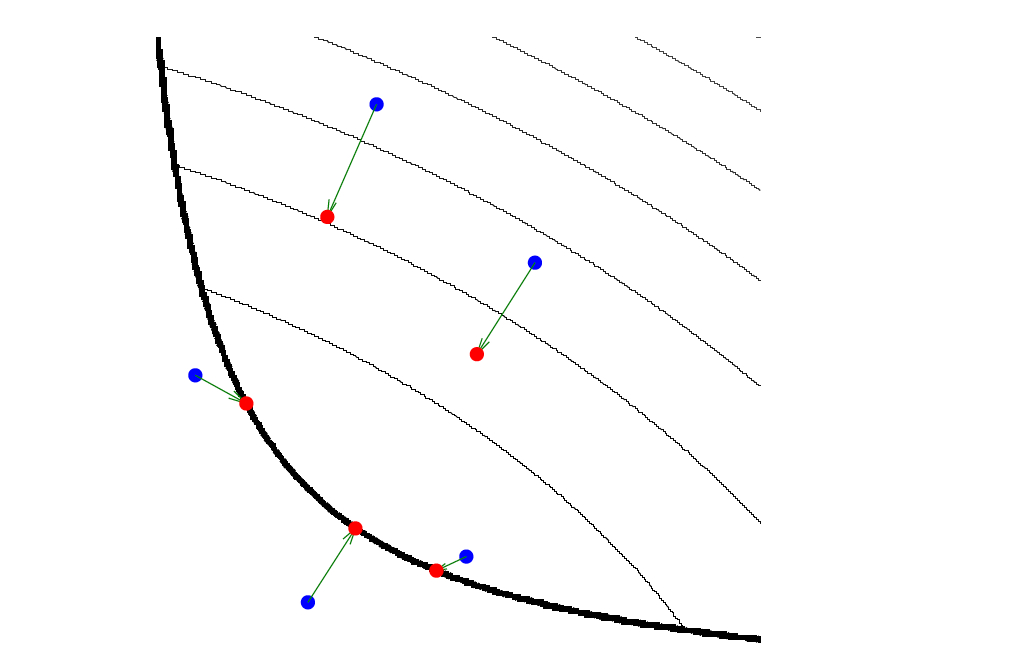
\includegraphics[width = 0.5\textwidth]{graphics/prox_boyd.jpg}
			\caption{\footnotesize Evaluating a proximal operator at various points. \textit{N Parikh, S Boyd, Proximal Methods,
					Foundations and Trends in Optimization 1, 2014}}
		\end{figure} 	
   \end{frame}
   
   \begin{frame}{Proximal Method: Zero-Memory Rank-One Update}
   	\alert{Traditional Proximal Gradient Step:}
   	\begin{equation*}
   	x_{k+1} = \prox_{\lambda_kh}(x_k - \lambda_k\nabla f(x_k))
   	\end{equation*}
   	\alert{Quasi-Newton Proximal Step:}
   	\begin{equation*}
   	x_{k+1} = \prox_h^{B_k}(x_k - B_k^{-1}\nabla f(x_k)),
   	\end{equation*}
   	with $B_k = \underbrace{D_k}_{diag} + \underbrace{u_k}_{\in\mathbb{R}^n}u_k^T$.\\
   	\vspace{5pt}
   	A zero-memory approach is used
   \end{frame}
   
   \begin{frame}{Proximal Method: Performance I}
   	\begin{columns}[T]
   		\begin{column}{.5\textwidth}
   			$F(x) = \lVert Ax - b \rVert + \lambda \lVert x \rVert_1$\\
   			$A \in \mathbb{R}^{1500 \times 3000},\:b \in \mathbb{R}^{1500}$\\
   			$A_{ij},\:b_i\:$ \textasciitilde $\:\mathcal{N}(0,1)$, $\:\lambda = 0.1$\\
   			\vspace{15pt}
   			\resizebox{\linewidth}{!}{% This file was created by matplotlib v0.1.0.
% Copyright (c) 2010--2014, Nico Schl�mer <nico.schloemer@gmail.com>
% All rights reserved.
% 
% The lastest updates can be retrieved from
% 
% https://github.com/nschloe/matplotlib2tikz
% 
% where you can also submit bug reports and leavecomments.
% 
\begin{tikzpicture}

\begin{axis}[
xlabel={Number of Iterations},
ylabel={Function Value},
xmin=0, xmax=55,
ymin=10, ymax=10000000000000,
ymode=log,
axis on top,
legend entries={{0SR1},{ProxGrad},{L-BFGS-B}}
]
\addplot [thick, red]
coordinates {
(0,23930.000884189)
(1,2334714540827.73)
(2,1603.06839363472)
(3,1004.45275331694)
(4,588.495767390219)
(5,2465.40475724742)
(6,179.594821649387)
(7,126.10021752328)
(8,61.4875604431263)
(9,129.281440688095)
(10,45.4082629909795)
(11,42.394874463473)
(12,119.624730091399)
(13,51.1689226777425)
(14,32.9092659784772)
(15,29.0693418166155)
(16,56.3092645316347)
(17,42.3296301168754)
(18,26.0389860835202)
(19,24.072093333035)
(20,29.9753713640302)
(21,34.7565678982828)
(22,21.2930785912614)
(23,20.2111387939323)
(24,27.3668342566393)
(25,19.5107974611296)
(26,18.4848613019356)
(27,18.2334402824762)
(28,18.3815429335346)
(29,18.8034834674539)
(30,17.87043345129)
(31,17.8003210729537)
(32,18.0911346039328)
(33,17.8675588710352)
(34,17.6897872539639)
(35,17.657870704215)
(36,17.7868354702454)
(37,17.6638138927485)
(38,17.6029421873073)
(39,17.5857582401889)
(40,17.593531318576)
(41,17.6173728315327)
(42,17.5451975095162)
(43,17.5349437987365)
(44,17.5463738339233)
(45,17.5615379779338)
(46,17.5098254996569)
(47,17.502148251481)
(48,17.5255046093324)
(49,17.51125728217)
(50,17.4770773904264)
(51,17.4669089400231)
(52,17.4917281760979)
(53,17.4651780471754)
(54,17.446393502165)
(55,17.4367726172038)

};
\addplot [thick, blue]
coordinates {
(0,23930.000884189)
(1,7180.45388604586)
(2,3617.86527996726)
(3,2206.80793392946)
(4,1491.00767628939)
(5,1073.99586354884)
(6,808.278854547473)
(7,628.014922400163)
(8,499.960644278589)
(9,405.752764676303)
(10,334.52634655712)
(11,279.477813847677)
(12,236.164491398145)
(13,201.577684383878)
(14,173.611856832551)
(15,150.754899712087)
(16,131.896367104543)
(17,116.20926011348)
(18,103.06516983272)
(19,91.9789779656275)
(20,82.5721972749523)
(21,74.5480919899652)
(22,67.6703468931341)
(23,61.7492516151206)
(24,56.6308080266971)
(25,52.1895417181108)
(26,48.3230738518772)
(27,44.9473811889776)
(28,41.9908958545994)
(29,39.3943307887263)
(30,37.1076648133911)
(31,35.0895582332656)
(32,33.3047098499916)
(33,31.7230458561848)
(34,30.3185369243055)
(35,29.0691392036425)
(36,27.9557168948839)
(37,26.9619473758925)
(38,26.0735819006833)
(39,25.2785051309949)
(40,24.5658953302441)
(41,23.9261996677162)
(42,23.3512128923731)
(43,22.8338555363931)
(44,22.3679803523897)
(45,21.9478508869475)
(46,21.5686369463874)
(47,21.2260325999356)
(48,20.9161983824383)
(49,20.6357394037178)
(50,20.3816052485759)
(51,20.1511846245288)
(52,19.942073913322)
(53,19.7522963849272)
(54,19.5798157329886)
(55,19.4229051369124)

};
\addplot [thick, green!50.0!black]
coordinates {
(0,23930.000884189)
(1,12083.1529253535)
(2,1962.70076992746)
(3,950.485602345173)
(4,331.959633328347)
(5,243.914762566925)
(6,134.329835058351)
(7,101.908974098636)
(8,71.430490269532)
(9,53.8008057292489)
(10,49.2070909809805)
(11,47.2377989642264)
(12,45.8394992598531)
(13,44.9246042975355)
(14,44.7440629754329)
(15,44.39329787842)
(16,44.3236229723654)
(17,44.2184239820041)
(18,44.1931882049634)
(19,44.1267629597911)
(20,44.1051433432534)
(21,44.0736620641302)
(22,44.0227863049802)
(23,43.9604053846835)
(24,43.8383240409788)
(25,43.7012466950384)
(26,43.4900906898139)
(27,43.1528664627698)
(28,42.5004315629993)
(29,41.8013543791512)
(30,40.8296742339329)
(31,39.900023272227)
(32,38.5823534699433)
(33,37.4156430458995)
(34,36.2719668390337)
(35,35.0776601950381)
(36,34.1837687644875)
(37,33.2698645775237)
(38,32.1962015032741)
(39,31.3082549503913)
(40,30.4262826422634)
(41,29.5345560514281)
(42,28.6995811800974)
(43,27.8507440638526)
(44,26.8903832876716)
(45,26.0249848856949)
(46,25.0716863775733)
(47,24.1555764755733)
(48,23.4070450974266)
(49,22.7049953977644)
(50,22.0172886765464)
(51,21.3371046021488)
(52,20.6002987471974)
(53,19.9394587462096)
(54,19.3137752887323)
(55,18.6682287336718)
(56,18.1127667913341)

};
\path [draw=black, fill opacity=0] (axis cs:13,1)--(axis cs:13,1);

\path [draw=black, fill opacity=0] (axis cs:1,13)--(axis cs:1,13);

\path [draw=black, fill opacity=0] (axis cs:13,0)--(axis cs:13,0);

\path [draw=black, fill opacity=0] (axis cs:0,13)--(axis cs:0,13);

\end{axis}

\end{tikzpicture}}
   			\begin{center}
   				\hspace{-3pt}
   				\scalebox{0.85}{
   					\begin{tabular}{|c|c|c|c|}
   						\hline                       
   						&\tiny \textbf{0SR1} & \tiny \textbf{ProxGrad} &  \tiny \textbf{L-BFGS-B} \\ \hline
   						\tiny \textbf{Iterations} &\tiny  1,822	& \tiny 135,328 & \tiny 1,989 \\	\hline  
   						\tiny \textbf{Run-Time}&\tiny 68 s & \tiny 1,144 s &\tiny 56 s  \\ \hline
   						
   					\end{tabular}
   				}
   			\end{center}
   		
   		\end{column}\hfill
   		\begin{column}{.5\textwidth}
   			$F(x) = \lVert Ax - b \rVert + \lambda \lVert x \rVert_1$\\
   			$A \in \mathbb{R}^{2197 \times 2197},\:b \in \mathbb{R}^{2197}$\\
   			$A$: \small Discretization of 3D Laplacian\\
   			\normalsize$\lambda = 1$\\
   			\vspace{8pt}
   			\resizebox{\linewidth}{!}{% This file was created by matplotlib v0.1.0.
% Copyright (c) 2010--2014, Nico Schl�mer <nico.schloemer@gmail.com>
% All rights reserved.
% 
% The lastest updates can be retrieved from
% 
% https://github.com/nschloe/matplotlib2tikz
% 
% where you can also submit bug reports and leavecomments.
% 
\begin{tikzpicture}

\begin{axis}[
xlabel={Number of Iterations},
ylabel={Function Value},
xmin=0, xmax=20,
ymin=1e-06, ymax=1000,
ymode=log,
axis on top,
legend entries={{0SR1},{ProxGrad},{L-BFGS-B}}
]
\addplot [thick, red]
coordinates {
(0,344.947171722221)
(1,344.947171722221)
(2,221.971344823809)
(3,105.183268059287)
(4,24.0246493050018)
(5,3.8316429574547)
(6,0.305853582808667)
(7,6.51020674248988e-06)

};
\addplot [thick, blue]
coordinates {
(0,344.947171722221)
(1,344.947171722221)
(2,221.971344823809)
(3,175.170522815298)
(4,145.915190646345)
(5,123.149864486456)
(6,103.386318060267)
(7,85.3055719850904)
(8,68.406762409266)
(9,52.6898461102236)
(10,38.4654743969608)
(11,26.1480751713354)
(12,16.2522156714462)
(13,9.06963280069867)
(14,4.51898312593936)
(15,1.90484081417415)
(16,0.662798369115754)
(17,0.178159154163643)
(18,0.0227851397424546)
(19,6.51020673590862e-06)

};
\addplot [thick, green!50.0!black]
coordinates {
(0,344.947171722221)
(1,344.947171722221)
(2,270.178125308224)
(3,230.58345596282)
(4,168.055709656042)
(5,53.7596820510628)
(6,11.3958775990856)
(7,1.34840826948498)
(8,0.267676178235767)
(9,0.0778255109435076)
(10,0.046406987419385)
(11,6.51020673590862e-06)

};
\path [draw=black, fill opacity=0] (axis cs:13,0)--(axis cs:13,0);

\path [draw=black, fill opacity=0] (axis cs:13,1)--(axis cs:13,1);

\path [draw=black, fill opacity=0] (axis cs:0,13)--(axis cs:0,13);

\path [draw=black, fill opacity=0] (axis cs:1,13)--(axis cs:1,13);

\end{axis}

\end{tikzpicture}}
   			\begin{center}
   				\hspace{5pt}
   				\scalebox{0.85}{
   					\begin{tabular}{|c|c|c|c|}
   						\hline                       
   						&\tiny \textbf{0SR1} & \tiny \textbf{ProxGrad} &  \tiny \textbf{L-BFGS-B} \\ \hline
   						\tiny \textbf{Iterations}& \tiny  7	& \tiny 18 & \tiny 10 \\	\hline  
   						\tiny \textbf{Run-Time}& \tiny 0.037 s &\tiny 0.004 s &\tiny 0.022 s\\ \hline
   						
   					\end{tabular}
   				}
   			\end{center}
   		\end{column}
   	\end{columns}
   \end{frame}
   
   \begin{frame}{Proximal Method: Stochastic Extension}
   High-dimensional data:
   Extension to stochastic framework\\
   \vspace{25pt}
   \centering\alert{Effect of batch size}
   	\begin{columns}[T]
   		\hspace{-16pt}
   		\begin{column}{.3\textwidth}
   			\hspace{30pt} \scriptsize Batch size = 1
   			\vspace{10pt}
   			\resizebox{1.18\linewidth}{!}{% This file was created by matplotlib v0.1.0.
% Copyright (c) 2010--2014, Nico Schl�mer <nico.schloemer@gmail.com>
% All rights reserved.
% 
% The lastest updates can be retrieved from
% 
% https://github.com/nschloe/matplotlib2tikz
% 
% where you can also submit bug reports and leavecomments.
% 
\begin{tikzpicture}

\begin{axis}[
xlabel={Number of Iterations},
ylabel={Function Value},
xmin=0, xmax=100,
ymin=1, ymax=100000,
ymode=log,
axis on top,
legend entries={{0SR1},{PG},{S0SR1},{SPG}}
]
\addplot [thick, red]
coordinates {
(0,23930.000884189)
(1,7180.45388604586)
(2,1602.10980923053)
(3,580.81114454538)
(4,519.996842220967)
(5,203.222944097077)
(6,121.922299073436)
(7,51.6523543005163)
(8,59.2695972484554)
(9,30.819611673989)
(10,25.614751730395)
(11,21.7592732486774)
(12,22.654003528062)
(13,20.15049001864)
(14,19.850460675318)
(15,18.3912111072782)
(16,23.73822362313)
(17,17.8866027335036)
(18,17.8196671916423)
(19,17.7775123499805)
(20,18.0615078838142)
(21,17.7506027746239)
(22,17.7424949039984)
(23,17.7297358775166)
(24,18.0476551294605)
(25,17.7168284338285)
(26,17.7118227102102)
(27,17.897336767244)
(28,17.7264425474283)
(29,17.6583909070735)
(30,17.6466963489978)
(31,17.5726603204587)
(32,17.9785494963624)
(33,17.5007993751903)
(34,17.4774762719696)
(35,17.4693572907426)
(36,18.0844886660129)
(37,17.4544077868014)
(38,17.4488948638463)
(39,17.3764214969115)
(40,17.5899917220372)
(41,17.1689206218387)
(42,17.0926131263914)
(43,17.193691075103)
(44,19.0707895757655)
(45,16.9630825309593)
(46,16.9036371416858)
(47,16.8413981063643)
(48,16.8743377801165)
(49,16.6801578404075)
(50,16.5909092149981)
(51,15.9390711318578)
(52,15.2212036355576)
(53,13.1777255991126)
(54,11.3509943341348)
(55,10.0944946484959)
(56,9.71465222794144)
(57,9.40843618327981)
(58,9.31008072896225)
(59,9.12293542675185)
(60,8.97211792181375)
(61,9.96955580951941)
(62,8.8971778312592)
(63,8.89032770510936)
(64,8.846532027156)
(65,9.14275424383174)
(66,8.76428614407871)
(67,8.74549967678879)
(68,8.81264423855369)
(69,8.92224051152909)
(70,8.71372433712952)
(71,8.69686120584995)
(72,8.86066032777056)
(73,8.64994348063148)
(74,8.64177834237841)
(75,8.61074429525064)
(76,8.97413158797716)
(77,8.57239195780947)
(78,8.56084322589053)
(79,8.56535473569669)
(80,8.70378144008176)
(81,8.55111754917089)
(82,8.54693544975204)
(83,8.66605947747419)
(84,8.49089417601578)
(85,8.48541554539908)
(86,8.44561206967175)
(87,8.58014556574557)
(88,8.40335231266141)
(89,8.3639219974089)
(90,8.30542294510122)
(91,8.53249537616582)
(92,8.29202808913906)
(93,8.25359007491097)
(94,8.22495187877562)
(95,8.2493220091081)
(96,8.31589617161871)
(97,8.19976279420752)
(98,8.18967260723272)
(99,8.37069393810889)
(100,8.23037470713979)

};
\addplot [thick, blue]
coordinates {
(0,23930.000884189)
(1,7180.45388604586)
(2,3617.86527996726)
(3,2206.80793392946)
(4,1491.00767628939)
(5,1073.99586354884)
(6,808.278854547473)
(7,628.014922400163)
(8,499.960644278589)
(9,405.752764676303)
(10,334.52634655712)
(11,279.477813847677)
(12,236.164491398145)
(13,201.577684383878)
(14,173.611856832551)
(15,150.754899712087)
(16,131.896367104543)
(17,116.20926011348)
(18,103.06516983272)
(19,91.9789779656275)
(20,82.5721972749523)
(21,74.5480919899652)
(22,67.6703468931341)
(23,61.7492516151206)
(24,56.6308080266971)
(25,52.1895417181108)
(26,48.3230738518772)
(27,44.9473811889776)
(28,41.9908958545994)
(29,39.3943307887263)
(30,37.1076648133911)
(31,35.0895582332656)
(32,33.3047098499916)
(33,31.7230458561848)
(34,30.3185369243055)
(35,29.0691392036425)
(36,27.9557168948839)
(37,26.9619473758925)
(38,26.0735819006833)
(39,25.2785051309949)
(40,24.5658953302441)
(41,23.9261996677162)
(42,23.3512128923731)
(43,22.8338555363931)
(44,22.3679803523897)
(45,21.9478508869475)
(46,21.5686369463874)
(47,21.2260325999356)
(48,20.9161983824383)
(49,20.6357394037178)
(50,20.3816052485759)
(51,20.1511846245288)
(52,19.942073913322)
(53,19.7522963849272)
(54,19.5798157329886)
(55,19.4229051369124)
(56,19.2800427060627)
(57,19.1499227239291)
(58,19.0313113044641)
(59,18.9230788312623)
(60,18.8242439624631)
(61,18.7339264319528)
(62,18.6513238709167)
(63,18.5757271356125)
(64,18.5064950547755)
(65,18.4430397931058)
(66,18.3848534199294)
(67,18.3314621000904)
(68,18.282410130483)
(69,18.2373078847479)
(70,18.195837809721)
(71,18.1576476003302)
(72,18.1224457540708)
(73,18.0899698163812)
(74,18.0599809133384)
(75,18.032269842075)
(76,18.0066439340179)
(77,17.9829130684296)
(78,17.9609160188493)
(79,17.9405020453336)
(80,17.9215358365279)
(81,17.9038985280102)
(82,17.8874801575507)
(83,17.8721768211419)
(84,17.8578894936326)
(85,17.8445328788038)
(86,17.83202928813)
(87,17.8203078087826)
(88,17.8093094635342)
(89,17.7989701384791)
(90,17.7892345518416)
(91,17.7800530702916)
(92,17.7713803468455)
(93,17.7631748927227)
(94,17.755398724103)
(95,17.7480170503084)
(96,17.7409979934438)
(97,17.7343123346806)
(98,17.7279332839925)
(99,17.7218362708545)
(100,17.7160071042362)

};
\addplot [thick, green!50.0!black]
coordinates {
(0,23930.000884189)
(1,23923.334047724)
(2,23928.7635276026)
(3,23903.2228942111)
(4,23880.551116968)
(5,23870.1438694121)
(6,23840.8591097331)
(7,23800.5465231594)
(8,23693.5652072578)
(9,23631.2019253979)
(10,23595.7049294721)
(11,23557.3218465756)
(12,23539.2186492497)
(13,23473.584727042)
(14,23400.1812437473)
(15,23388.0720749918)
(16,23318.1474310779)
(17,23292.0698546307)
(18,23269.068415991)
(19,23210.8791988646)
(20,23193.4863330836)
(21,23181.6599796314)
(22,23062.4792306439)
(23,23035.3733843549)
(24,23032.8599854377)
(25,22939.6846047895)
(26,22929.2618733069)
(27,22867.1481481817)
(28,22818.677731829)
(29,22807.9258198671)
(30,22785.6420041927)
(31,22755.6532908351)
(32,22742.582665471)
(33,22725.8825926485)
(34,22684.1564937657)
(35,22606.4456396911)
(36,22572.1742036179)
(37,22554.3985911884)
(38,22522.8369496402)
(39,22469.3743043561)
(40,22448.1243780356)
(41,22414.5732307433)
(42,22391.7091715499)
(43,22379.7010436894)
(44,22323.1997260491)
(45,22288.681718955)
(46,22282.2596286649)
(47,22284.2692515112)
(48,22235.9625129174)
(49,22213.2722470128)
(50,22178.9652092496)
(51,22157.7238236404)
(52,22153.6879665373)
(53,22140.6889877556)
(54,22123.4074016335)
(55,22116.046144858)
(56,22111.9024374621)
(57,22105.9198104965)
(58,21964.1343917105)
(59,21929.7826902415)
(60,21919.2485920075)
(61,21830.9844862054)
(62,21821.6299921176)
(63,21808.0503615675)
(64,21797.9385095849)
(65,21784.6608946421)
(66,21769.8680785984)
(67,21748.6833833625)
(68,21674.4511468646)
(69,21661.9376809697)
(70,21507.9874738557)
(71,21486.1511327575)
(72,21443.970383019)
(73,21439.7646878615)
(74,21420.0980397293)
(75,21306.20071164)
(76,21273.4158974333)
(77,21230.9495093902)
(78,21220.6918082251)
(79,21209.498741541)
(80,21178.4949344347)
(81,21162.2436290185)
(82,21141.5973807421)
(83,21101.8211631996)
(84,21032.6648578308)
(85,21024.2079580824)
(86,20999.327086295)
(87,20968.6752743001)
(88,20931.3260880202)
(89,20886.1066199987)
(90,20863.1270327032)
(91,20850.5835406883)
(92,20791.7487241044)
(93,20780.2586328704)
(94,20667.450523141)
(95,20436.9578418679)
(96,20321.419385273)
(97,20306.0602165487)
(98,20230.0396648291)
(99,20199.7871509236)
(100,20187.8616636121)

};
\addplot [thick, black]
coordinates {
(0,23930.000884189)
(1,23890.7203112094)
(2,23878.2170334922)
(3,23872.9686180075)
(4,23866.5346978871)
(5,23850.8764373553)
(6,23787.6950107308)
(7,23775.2516717042)
(8,23762.1300268247)
(9,23748.3910080289)
(10,23742.4176277215)
(11,23737.2794479725)
(12,23712.9424883472)
(13,23708.2694816423)
(14,23695.5428051205)
(15,23690.6246255974)
(16,23687.9657700372)
(17,23682.3953826871)
(18,23653.6012341404)
(19,23649.4236352872)
(20,23604.2971428242)
(21,23599.4062344063)
(22,23569.6297513714)
(23,23556.0011900061)
(24,23549.9773609808)
(25,23537.2426445563)
(26,23525.0819362898)
(27,23517.6903376486)
(28,23494.4847770765)
(29,23488.1010901902)
(30,23464.1734774381)
(31,23458.8655867368)
(32,23456.126867557)
(33,23441.5265289338)
(34,23436.4208834939)
(35,23401.2764127029)
(36,23372.2130357179)
(37,23345.1245749014)
(38,23335.6753012462)
(39,23302.2316059798)
(40,23293.8727188189)
(41,23296.2855197425)
(42,23277.2518022093)
(43,23248.185842466)
(44,23227.8846968562)
(45,23211.1802037091)
(46,23165.8983053437)
(47,23144.5178907953)
(48,23134.0165866522)
(49,23107.3347892962)
(50,23099.1373874557)
(51,23072.4548553106)
(52,23067.2888466665)
(53,23054.9606379638)
(54,23044.7351663614)
(55,23037.7511586)
(56,23032.536131999)
(57,23013.8989655525)
(58,22993.535118503)
(59,22988.6210309045)
(60,22981.4397361105)
(61,22976.4924591746)
(62,22971.6682267528)
(63,22967.0362740143)
(64,22961.8842584499)
(65,22879.4871764632)
(66,22870.2420512314)
(67,22869.5838747355)
(68,22859.9466968665)
(69,22854.4506719323)
(70,22833.5518644733)
(71,22829.9975916655)
(72,22749.1493997893)
(73,22738.4968508306)
(74,22722.0365538912)
(75,22717.4156339043)
(76,22701.8070654364)
(77,22699.1574630432)
(78,22640.8706502276)
(79,22636.8312482253)
(80,22622.284223347)
(81,22544.9797946472)
(82,22536.1429896047)
(83,22529.6266187036)
(84,22524.6932752277)
(85,22512.0230096588)
(86,22493.5562713872)
(87,22442.2856687459)
(88,22432.8918264189)
(89,22391.350837251)
(90,22345.9832234223)
(91,22259.3110049608)
(92,22253.2353619672)
(93,22206.5548772089)
(94,22200.5719097136)
(95,22186.6237812275)
(96,22161.1787011814)
(97,22140.2994978854)
(98,22134.8075457781)
(99,22124.9060394855)
(100,22121.1279874691)

};
\path [draw=black, fill opacity=0] (axis cs:1,13)--(axis cs:1,13);

\path [draw=black, fill opacity=0] (axis cs:13,0)--(axis cs:13,0);

\path [draw=black, fill opacity=0] (axis cs:13,1)--(axis cs:13,1);

\path [draw=black, fill opacity=0] (axis cs:0,13)--(axis cs:0,13);

\end{axis}

\end{tikzpicture}}
   		\end{column}\hspace{-16pt}
   		\begin{column}{.3\textwidth}
   			\hspace{30pt} \scriptsize Batch size = 50
   			\vspace{10pt}
   			\resizebox{1.18\linewidth}{!}{% This file was created by matplotlib v0.1.0.
% Copyright (c) 2010--2014, Nico Schl�mer <nico.schloemer@gmail.com>
% All rights reserved.
% 
% The lastest updates can be retrieved from
% 
% https://github.com/nschloe/matplotlib2tikz
% 
% where you can also submit bug reports and leavecomments.
% 
\begin{tikzpicture}

\begin{axis}[
xlabel={Number of Iterations},
ylabel={Function Value},
xmin=0, xmax=100,
ymin=1, ymax=100000,
ymode=log,
axis on top,
legend entries={{0SR1},{PG},{S0SR1},{SPG}}
]
\addplot [thick, red]
coordinates {
(0,23930.000884189)
(1,7180.45388604586)
(2,1602.10980923053)
(3,580.81114454538)
(4,519.996842220967)
(5,203.222944097077)
(6,121.922299073436)
(7,51.6523543005163)
(8,59.2695972484554)
(9,30.819611673989)
(10,25.614751730395)
(11,21.7592732486774)
(12,22.654003528062)
(13,20.15049001864)
(14,19.850460675318)
(15,18.3912111072782)
(16,23.73822362313)
(17,17.8866027335036)
(18,17.8196671916423)
(19,17.7775123499805)
(20,18.0615078838142)
(21,17.7506027746239)
(22,17.7424949039984)
(23,17.7297358775166)
(24,18.0476551294605)
(25,17.7168284338285)
(26,17.7118227102102)
(27,17.897336767244)
(28,17.7264425474283)
(29,17.6583909070735)
(30,17.6466963489978)
(31,17.5726603204587)
(32,17.9785494963624)
(33,17.5007993751903)
(34,17.4774762719696)
(35,17.4693572907426)
(36,18.0844886660129)
(37,17.4544077868014)
(38,17.4488948638463)
(39,17.3764214969115)
(40,17.5899917220372)
(41,17.1689206218387)
(42,17.0926131263914)
(43,17.193691075103)
(44,19.0707895757655)
(45,16.9630825309593)
(46,16.9036371416858)
(47,16.8413981063643)
(48,16.8743377801165)
(49,16.6801578404075)
(50,16.5909092149981)
(51,15.9390711318578)
(52,15.2212036355576)
(53,13.1777255991126)
(54,11.3509943341348)
(55,10.0944946484959)
(56,9.71465222794144)
(57,9.40843618327981)
(58,9.31008072896225)
(59,9.12293542675185)
(60,8.97211792181375)
(61,9.96955580951941)
(62,8.8971778312592)
(63,8.89032770510936)
(64,8.846532027156)
(65,9.14275424383174)
(66,8.76428614407871)
(67,8.74549967678879)
(68,8.81264423855369)
(69,8.92224051152909)
(70,8.71372433712952)
(71,8.69686120584995)
(72,8.86066032777056)
(73,8.64994348063148)
(74,8.64177834237841)
(75,8.61074429525064)
(76,8.97413158797716)
(77,8.57239195780947)
(78,8.56084322589053)
(79,8.56535473569669)
(80,8.70378144008176)
(81,8.55111754917089)
(82,8.54693544975204)
(83,8.66605947747419)
(84,8.49089417601578)
(85,8.48541554539908)
(86,8.44561206967175)
(87,8.58014556574557)
(88,8.40335231266141)
(89,8.3639219974089)
(90,8.30542294510122)
(91,8.53249537616582)
(92,8.29202808913906)
(93,8.25359007491097)
(94,8.22495187877562)
(95,8.2493220091081)
(96,8.31589617161871)
(97,8.19976279420752)
(98,8.18967260723272)
(99,8.37069393810889)
(100,8.23037470713979)

};
\addplot [thick, blue]
coordinates {
(0,23930.000884189)
(1,7180.45388604586)
(2,3617.86527996726)
(3,2206.80793392946)
(4,1491.00767628939)
(5,1073.99586354884)
(6,808.278854547473)
(7,628.014922400163)
(8,499.960644278589)
(9,405.752764676303)
(10,334.52634655712)
(11,279.477813847677)
(12,236.164491398145)
(13,201.577684383878)
(14,173.611856832551)
(15,150.754899712087)
(16,131.896367104543)
(17,116.20926011348)
(18,103.06516983272)
(19,91.9789779656275)
(20,82.5721972749523)
(21,74.5480919899652)
(22,67.6703468931341)
(23,61.7492516151206)
(24,56.6308080266971)
(25,52.1895417181108)
(26,48.3230738518772)
(27,44.9473811889776)
(28,41.9908958545994)
(29,39.3943307887263)
(30,37.1076648133911)
(31,35.0895582332656)
(32,33.3047098499916)
(33,31.7230458561848)
(34,30.3185369243055)
(35,29.0691392036425)
(36,27.9557168948839)
(37,26.9619473758925)
(38,26.0735819006833)
(39,25.2785051309949)
(40,24.5658953302441)
(41,23.9261996677162)
(42,23.3512128923731)
(43,22.8338555363931)
(44,22.3679803523897)
(45,21.9478508869475)
(46,21.5686369463874)
(47,21.2260325999356)
(48,20.9161983824383)
(49,20.6357394037178)
(50,20.3816052485759)
(51,20.1511846245288)
(52,19.942073913322)
(53,19.7522963849272)
(54,19.5798157329886)
(55,19.4229051369124)
(56,19.2800427060627)
(57,19.1499227239291)
(58,19.0313113044641)
(59,18.9230788312623)
(60,18.8242439624631)
(61,18.7339264319528)
(62,18.6513238709167)
(63,18.5757271356125)
(64,18.5064950547755)
(65,18.4430397931058)
(66,18.3848534199294)
(67,18.3314621000904)
(68,18.282410130483)
(69,18.2373078847479)
(70,18.195837809721)
(71,18.1576476003302)
(72,18.1224457540708)
(73,18.0899698163812)
(74,18.0599809133384)
(75,18.032269842075)
(76,18.0066439340179)
(77,17.9829130684296)
(78,17.9609160188493)
(79,17.9405020453336)
(80,17.9215358365279)
(81,17.9038985280102)
(82,17.8874801575507)
(83,17.8721768211419)
(84,17.8578894936326)
(85,17.8445328788038)
(86,17.83202928813)
(87,17.8203078087826)
(88,17.8093094635342)
(89,17.7989701384791)
(90,17.7892345518416)
(91,17.7800530702916)
(92,17.7713803468455)
(93,17.7631748927227)
(94,17.755398724103)
(95,17.7480170503084)
(96,17.7409979934438)
(97,17.7343123346806)
(98,17.7279332839925)
(99,17.7218362708545)
(100,17.7160071042362)

};
\addplot [thick, green!50.0!black]
coordinates {
(0,23930.000884189)
(1,23171.0346959744)
(2,21784.3535900778)
(3,20501.4769070109)
(4,19543.6665497666)
(5,18988.7934814984)
(6,18215.4373574971)
(7,17272.1454863206)
(8,16427.6602658124)
(9,15867.5434466811)
(10,14894.918119963)
(11,14116.9994755899)
(12,13726.9429460544)
(13,13327.6846049478)
(14,12811.0074148469)
(15,12439.6946147915)
(16,11982.3722133073)
(17,11569.3180134221)
(18,11039.307674824)
(19,10658.5139274633)
(20,10233.3532190102)
(21,9830.49141422135)
(22,9538.50386463762)
(23,9292.46215015677)
(24,8922.53723282377)
(25,8689.62695889746)
(26,8332.21531651746)
(27,8060.22179928855)
(28,7542.81062742628)
(29,7345.62352876317)
(30,7122.59280048562)
(31,6911.71867839273)
(32,6783.96852282346)
(33,6597.39813805498)
(34,6421.08199318435)
(35,6051.4440357494)
(36,5864.06903393834)
(37,5710.841520059)
(38,5465.94544022695)
(39,5295.42752247915)
(40,5083.37809781545)
(41,5014.56044826766)
(42,4956.89249180127)
(43,4798.11876413539)
(44,4767.91069849755)
(45,4619.00590806872)
(46,4538.59417059465)
(47,4433.87381330478)
(48,4343.63399486368)
(49,4249.49366868748)
(50,4147.51613532838)
(51,4008.73791472631)
(52,3920.33204121809)
(53,3799.16925271651)
(54,3724.07754306651)
(55,3652.86033114161)
(56,3609.46730550209)
(57,3390.97125217073)
(58,3290.83637561082)
(59,3241.56939297359)
(60,3127.06324030011)
(61,3051.82316650495)
(62,3019.50281905113)
(63,2962.39855462584)
(64,2879.09281679541)
(65,2821.50325676303)
(66,2754.65445009351)
(67,2716.91027069895)
(68,2612.14382872169)
(69,2563.32013516176)
(70,2520.70611327144)
(71,2476.5004250781)
(72,2374.27877130335)
(73,2344.16839504726)
(74,2312.75922747124)
(75,2277.12912174529)
(76,2269.54728601055)
(77,2205.90555954617)
(78,2147.79636872422)
(79,2123.52923930368)
(80,2097.70583017859)
(81,2079.83915939177)
(82,2001.2167455977)
(83,1958.97259960861)
(84,1932.49471599967)
(85,1910.78626157815)
(86,1888.27388183557)
(87,1822.21242558697)
(88,1787.25681803998)
(89,1737.2226512776)
(90,1724.81413377049)
(91,1698.50141287942)
(92,1664.30055132707)
(93,1632.82687249937)
(94,1557.6162509941)
(95,1522.83828155334)
(96,1464.39049704361)
(97,1433.11448377846)
(98,1417.71333251217)
(99,1407.86044704754)
(100,1344.81616763266)

};
\addplot [thick, black]
coordinates {
(0,23930.000884189)
(1,23293.1463670467)
(2,22553.387902309)
(3,21670.4864884541)
(4,20750.5513890745)
(5,20195.5275977338)
(6,19748.5819979135)
(7,19383.5430314739)
(8,18780.5418113084)
(9,18448.36860308)
(10,17959.6641837916)
(11,17442.0382999429)
(12,17013.0300143071)
(13,16529.8968496443)
(14,16056.6251422336)
(15,15808.1473900858)
(16,15491.2327974059)
(17,15160.0547738003)
(18,14839.8815790667)
(19,14475.8853962597)
(20,13994.7673749869)
(21,13735.2666879705)
(22,13271.7153440532)
(23,12772.5132825963)
(24,12495.3540557656)
(25,12171.4905558794)
(26,11963.292344086)
(27,11651.528551017)
(28,11303.7409235124)
(29,10950.1265296381)
(30,10684.058074616)
(31,10462.6972990673)
(32,10260.749041893)
(33,9942.4477782177)
(34,9755.90949540406)
(35,9543.06727328901)
(36,9375.21884479077)
(37,9225.93150626459)
(38,9017.44188999023)
(39,8700.02041152976)
(40,8572.1977841637)
(41,8416.28349705419)
(42,8243.77586374936)
(43,8012.48872705011)
(44,7896.27520735391)
(45,7771.15490274834)
(46,7695.1076200625)
(47,7583.17136596472)
(48,7333.10767096815)
(49,7186.55480315562)
(50,7042.13174645903)
(51,6973.849547127)
(52,6887.87235435164)
(53,6738.61901654716)
(54,6684.7944770361)
(55,6475.48700108552)
(56,6338.15776584224)
(57,6214.65158988481)
(58,6129.54348884943)
(59,6010.823316054)
(60,5869.57996643339)
(61,5761.15179212112)
(62,5708.69916893628)
(63,5622.76122546336)
(64,5544.05502537033)
(65,5478.69288104323)
(66,5403.22194656423)
(67,5341.90714131825)
(68,5222.34612750201)
(69,5121.1741698018)
(70,5087.49640237379)
(71,5014.18001774599)
(72,4899.9352399649)
(73,4822.63375697015)
(74,4742.89006151635)
(75,4677.02107086117)
(76,4592.91755663964)
(77,4530.91586617531)
(78,4420.99631661626)
(79,4376.80079193637)
(80,4279.9603821111)
(81,4227.02127969156)
(82,4188.01996451806)
(83,4138.89458389439)
(84,4074.734896419)
(85,3996.98838466048)
(86,3944.18752651912)
(87,3858.37275016319)
(88,3794.27356111269)
(89,3710.63525674627)
(90,3650.23006769274)
(91,3604.3861952728)
(92,3534.83163771068)
(93,3503.49394371603)
(94,3457.10600021213)
(95,3398.18132367632)
(96,3361.46674483991)
(97,3292.33317109272)
(98,3252.42254004838)
(99,3214.94409221704)
(100,3151.14396888867)

};
\path [draw=black, fill opacity=0] (axis cs:1,13)--(axis cs:1,13);

\path [draw=black, fill opacity=0] (axis cs:13,0)--(axis cs:13,0);

\path [draw=black, fill opacity=0] (axis cs:13,1)--(axis cs:13,1);

\path [draw=black, fill opacity=0] (axis cs:0,13)--(axis cs:0,13);

\end{axis}

\end{tikzpicture}}
   		\end{column}\hspace{-16pt}
   		\begin{column}{.3\textwidth}
   			\hspace{30pt} \scriptsize Batch size = 150
   			\vspace{10pt}
   			\resizebox{1.18\linewidth}{!}{% This file was created by matplotlib v0.1.0.
% Copyright (c) 2010--2014, Nico Schl�mer <nico.schloemer@gmail.com>
% All rights reserved.
% 
% The lastest updates can be retrieved from
% 
% https://github.com/nschloe/matplotlib2tikz
% 
% where you can also submit bug reports and leavecomments.
% 
\begin{tikzpicture}

\begin{axis}[
xlabel={Number of Iterations},
ylabel={Function Value},
xmin=0, xmax=100,
ymin=1, ymax=100000,
ymode=log,
axis on top,
legend entries={{0SR1},{PG},{S0SR1},{SPG}}
]
\addplot [thick, red]
coordinates {
(0,23930.000884189)
(1,7180.45388604586)
(2,1602.10980923053)
(3,580.81114454538)
(4,519.996842220967)
(5,203.222944097077)
(6,121.922299073436)
(7,51.6523543005163)
(8,59.2695972484554)
(9,30.819611673989)
(10,25.614751730395)
(11,21.7592732486774)
(12,22.654003528062)
(13,20.15049001864)
(14,19.850460675318)
(15,18.3912111072782)
(16,23.73822362313)
(17,17.8866027335036)
(18,17.8196671916423)
(19,17.7775123499805)
(20,18.0615078838142)
(21,17.7506027746239)
(22,17.7424949039984)
(23,17.7297358775166)
(24,18.0476551294605)
(25,17.7168284338285)
(26,17.7118227102102)
(27,17.897336767244)
(28,17.7264425474283)
(29,17.6583909070735)
(30,17.6466963489978)
(31,17.5726603204587)
(32,17.9785494963624)
(33,17.5007993751903)
(34,17.4774762719696)
(35,17.4693572907426)
(36,18.0844886660129)
(37,17.4544077868014)
(38,17.4488948638463)
(39,17.3764214969115)
(40,17.5899917220372)
(41,17.1689206218387)
(42,17.0926131263914)
(43,17.193691075103)
(44,19.0707895757655)
(45,16.9630825309593)
(46,16.9036371416858)
(47,16.8413981063643)
(48,16.8743377801165)
(49,16.6801578404075)
(50,16.5909092149981)
(51,15.9390711318578)
(52,15.2212036355576)
(53,13.1777255991126)
(54,11.3509943341348)
(55,10.0944946484959)
(56,9.71465222794144)
(57,9.40843618327981)
(58,9.31008072896225)
(59,9.12293542675185)
(60,8.97211792181375)
(61,9.96955580951941)
(62,8.8971778312592)
(63,8.89032770510936)
(64,8.846532027156)
(65,9.14275424383174)
(66,8.76428614407871)
(67,8.74549967678879)
(68,8.81264423855369)
(69,8.92224051152909)
(70,8.71372433712952)
(71,8.69686120584995)
(72,8.86066032777056)
(73,8.64994348063148)
(74,8.64177834237841)
(75,8.61074429525064)
(76,8.97413158797716)
(77,8.57239195780947)
(78,8.56084322589053)
(79,8.56535473569669)
(80,8.70378144008176)
(81,8.55111754917089)
(82,8.54693544975204)
(83,8.66605947747419)
(84,8.49089417601578)
(85,8.48541554539908)
(86,8.44561206967175)
(87,8.58014556574557)
(88,8.40335231266141)
(89,8.3639219974089)
(90,8.30542294510122)
(91,8.53249537616582)
(92,8.29202808913906)
(93,8.25359007491097)
(94,8.22495187877562)
(95,8.2493220091081)
(96,8.31589617161871)
(97,8.19976279420752)
(98,8.18967260723272)
(99,8.37069393810889)
(100,8.23037470713979)

};
\addplot [thick, blue]
coordinates {
(0,23930.000884189)
(1,7180.45388604586)
(2,3617.86527996726)
(3,2206.80793392946)
(4,1491.00767628939)
(5,1073.99586354884)
(6,808.278854547473)
(7,628.014922400163)
(8,499.960644278589)
(9,405.752764676303)
(10,334.52634655712)
(11,279.477813847677)
(12,236.164491398145)
(13,201.577684383878)
(14,173.611856832551)
(15,150.754899712087)
(16,131.896367104543)
(17,116.20926011348)
(18,103.06516983272)
(19,91.9789779656275)
(20,82.5721972749523)
(21,74.5480919899652)
(22,67.6703468931341)
(23,61.7492516151206)
(24,56.6308080266971)
(25,52.1895417181108)
(26,48.3230738518772)
(27,44.9473811889776)
(28,41.9908958545994)
(29,39.3943307887263)
(30,37.1076648133911)
(31,35.0895582332656)
(32,33.3047098499916)
(33,31.7230458561848)
(34,30.3185369243055)
(35,29.0691392036425)
(36,27.9557168948839)
(37,26.9619473758925)
(38,26.0735819006833)
(39,25.2785051309949)
(40,24.5658953302441)
(41,23.9261996677162)
(42,23.3512128923731)
(43,22.8338555363931)
(44,22.3679803523897)
(45,21.9478508869475)
(46,21.5686369463874)
(47,21.2260325999356)
(48,20.9161983824383)
(49,20.6357394037178)
(50,20.3816052485759)
(51,20.1511846245288)
(52,19.942073913322)
(53,19.7522963849272)
(54,19.5798157329886)
(55,19.4229051369124)
(56,19.2800427060627)
(57,19.1499227239291)
(58,19.0313113044641)
(59,18.9230788312623)
(60,18.8242439624631)
(61,18.7339264319528)
(62,18.6513238709167)
(63,18.5757271356125)
(64,18.5064950547755)
(65,18.4430397931058)
(66,18.3848534199294)
(67,18.3314621000904)
(68,18.282410130483)
(69,18.2373078847479)
(70,18.195837809721)
(71,18.1576476003302)
(72,18.1224457540708)
(73,18.0899698163812)
(74,18.0599809133384)
(75,18.032269842075)
(76,18.0066439340179)
(77,17.9829130684296)
(78,17.9609160188493)
(79,17.9405020453336)
(80,17.9215358365279)
(81,17.9038985280102)
(82,17.8874801575507)
(83,17.8721768211419)
(84,17.8578894936326)
(85,17.8445328788038)
(86,17.83202928813)
(87,17.8203078087826)
(88,17.8093094635342)
(89,17.7989701384791)
(90,17.7892345518416)
(91,17.7800530702916)
(92,17.7713803468455)
(93,17.7631748927227)
(94,17.755398724103)
(95,17.7480170503084)
(96,17.7409979934438)
(97,17.7343123346806)
(98,17.7279332839925)
(99,17.7218362708545)
(100,17.7160071042362)

};
\addplot [thick, green!50.0!black]
coordinates {
(0,23930.000884189)
(1,21975.8838823078)
(2,18879.7841116922)
(3,15960.0457997545)
(4,14447.1279373071)
(5,12820.1061318088)
(6,11421.3371094484)
(7,10030.9824217186)
(8,9262.35660898206)
(9,8585.4187508991)
(10,7688.96195002778)
(11,7132.34755549664)
(12,6525.2951182746)
(13,6027.09456653836)
(14,5597.23641138016)
(15,5187.22473075384)
(16,4772.05172482115)
(17,4471.68310363214)
(18,4209.37840725187)
(19,3983.04898585604)
(20,3667.91089385107)
(21,3482.61347510547)
(22,3204.98381841887)
(23,3005.41210512299)
(24,2789.48549555158)
(25,2596.21702301637)
(26,2432.36541193231)
(27,2273.67287544755)
(28,2121.48647499734)
(29,2027.04112150971)
(30,1967.84958661728)
(31,1893.26095480486)
(32,1827.94065349038)
(33,1742.67674887332)
(34,1620.77454333673)
(35,1554.37718117258)
(36,1459.00663185291)
(37,1367.10109079839)
(38,1272.10736049544)
(39,1203.39451094449)
(40,1106.49715073096)
(41,1057.04158786243)
(42,1008.40211835047)
(43,984.638316507915)
(44,958.578010233065)
(45,938.54976705447)
(46,898.464275861728)
(47,856.248510438271)
(48,782.28256338342)
(49,751.537914041033)
(50,735.781269501783)
(51,702.087572095052)
(52,670.348753496428)
(53,638.884372266288)
(54,618.771715950506)
(55,591.78179993537)
(56,553.545045310196)
(57,532.950511157198)
(58,525.270346627585)
(59,510.529645358556)
(60,478.261789311396)
(61,459.281523498543)
(62,441.941510943923)
(63,415.448885858652)
(64,408.870940091032)
(65,401.1861184411)
(66,375.52461046425)
(67,372.681837545989)
(68,360.648466528654)
(69,352.28337065206)
(70,329.30465767911)
(71,323.07630747367)
(72,307.498367140355)
(73,292.990481000015)
(74,282.478193315603)
(75,267.622742904421)
(76,264.93722965994)
(77,260.089696319324)
(78,250.507062682144)
(79,247.585988075163)
(80,242.134950230611)
(81,234.335317962934)
(82,220.50711900911)
(83,213.530194057356)
(84,213.158605459869)
(85,213.141689439488)
(86,209.134723198002)
(87,199.695600914175)
(88,191.479330978208)
(89,187.14012645406)
(90,183.283163341309)
(91,178.90686036297)
(92,176.978464251234)
(93,170.845146422236)
(94,160.318900295219)
(95,157.211520186089)
(96,155.730319261701)
(97,151.571310130795)
(98,147.790856841592)
(99,143.55714276405)
(100,139.731493391039)

};
\addplot [thick, black]
coordinates {
(0,23930.000884189)
(1,21965.7991947082)
(2,19839.111950648)
(3,18245.6603495555)
(4,16680.7461951488)
(5,15199.3720907056)
(6,14152.359426101)
(7,13249.1603187729)
(8,12106.876403638)
(9,11485.23537136)
(10,10624.0319832373)
(11,9998.23460040279)
(12,9422.70787630272)
(13,8821.25365208863)
(14,8245.35429931971)
(15,7889.63825592885)
(16,7451.142033771)
(17,6937.15210380027)
(18,6476.43919173826)
(19,6112.14465293491)
(20,5824.87229334082)
(21,5537.71260954863)
(22,5164.26550849617)
(23,4856.08827568902)
(24,4535.56040118895)
(25,4352.85351404823)
(26,4150.38773540579)
(27,3924.09232227433)
(28,3768.55661985695)
(29,3608.24629052429)
(30,3483.07998046816)
(31,3292.42823657164)
(32,3114.81719431215)
(33,2996.40682909122)
(34,2899.49477811012)
(35,2787.43820146127)
(36,2667.23824459715)
(37,2563.89074774176)
(38,2444.70473753739)
(39,2344.6641423738)
(40,2260.99267495662)
(41,2157.00635924888)
(42,2087.49262063616)
(43,2011.70388808009)
(44,1932.923696894)
(45,1885.79170445579)
(46,1829.26768287028)
(47,1771.93930339019)
(48,1682.8918326135)
(49,1629.22649488807)
(50,1591.83922210222)
(51,1556.38098178355)
(52,1508.11002119433)
(53,1462.74610811809)
(54,1431.13210322756)
(55,1366.41296056735)
(56,1333.16366228832)
(57,1299.31001305012)
(58,1263.86691844559)
(59,1234.98137203071)
(60,1204.51569914451)
(61,1164.96101924318)
(62,1120.26780370492)
(63,1100.66384629364)
(64,1076.0628189333)
(65,1044.44986761874)
(66,1014.34636686488)
(67,997.946852528628)
(68,961.128725048813)
(69,928.348639721778)
(70,909.686502121871)
(71,885.109210228062)
(72,861.830155219097)
(73,851.928861535559)
(74,827.245932841754)
(75,810.315966824559)
(76,788.915867943771)
(77,763.738854329862)
(78,742.715751501901)
(79,731.372101748885)
(80,704.591240684903)
(81,691.16383223837)
(82,674.66337409703)
(83,659.98195754727)
(84,648.240978785052)
(85,629.451397090187)
(86,616.966388764945)
(87,605.587561115596)
(88,599.04293861654)
(89,579.120434777272)
(90,571.689128156412)
(91,558.100643406932)
(92,545.52737212588)
(93,537.543618022914)
(94,528.687777844095)
(95,521.201881492171)
(96,512.015601796819)
(97,492.598839642987)
(98,480.437805137752)
(99,463.536973625467)
(100,458.21681935089)

};
\path [draw=black, fill opacity=0] (axis cs:1,13)--(axis cs:1,13);

\path [draw=black, fill opacity=0] (axis cs:13,0)--(axis cs:13,0);

\path [draw=black, fill opacity=0] (axis cs:13,1)--(axis cs:13,1);

\path [draw=black, fill opacity=0] (axis cs:0,13)--(axis cs:0,13);

\end{axis}

\end{tikzpicture}}
   		\end{column}
   	\end{columns}
   \end{frame}
   
   \begin{frame}{Proximal Method: Main Results}
   	\begin{itemize}
   		\item Superior results to standard proximal gradient
   		\item Competitive with other standard methods
   		\item Extension to stochastic framework possible
   		\item Applicable to large-scale problems
   	\end{itemize}
   \end{frame}

\section{Classification}

\plain{Electroencephalography (EEG)\\
	\vspace{10pt}
	\alert{How deep is your sleep?}
	\vspace{15pt}\\
	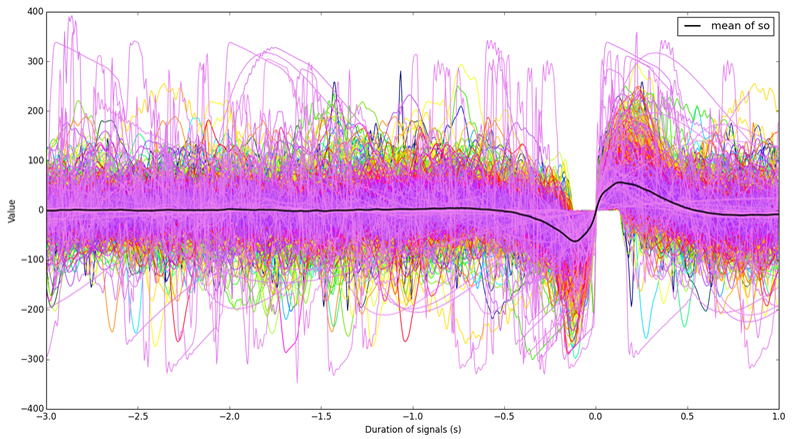
\includegraphics[width=0.7\textwidth]{graphics/EEG_oscillation.png}\\
	\vspace{15pt}
	\small Sleeping patient / 20 nights of EEG recordings\\
	\small Predict next slow wave
	}

  \begin{frame}\frametitle{Logistic Regression}
  $$ f(\omega, x_i, y_i) = -y_i \log(h(\omega,x_i)) - (1-y_i) \log(1- h(\omega, x_i))$$
  with
  $$h(\omega, x_i) := sigmoid(\omega^Tx_i):= \frac{1}{1+e^{-\omega^T x_i}} $$      

  \begin{figure}
  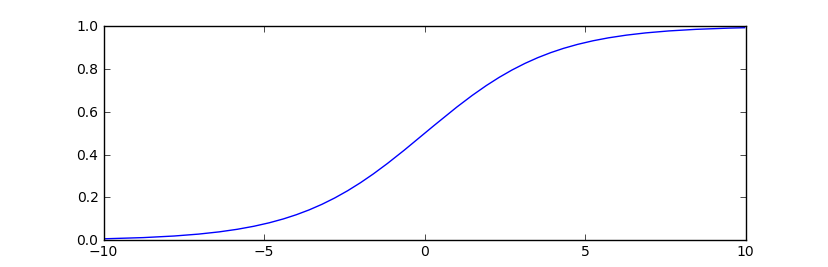
\includegraphics[width=.5\linewidth]{graphics/sigmoid.png}\caption{The sigmoid function.}
  \end{figure}
  
  \end{frame}

  
    	\begin{frame}{Classification: Results for SQN}
    		\begin{center}
    		\begin{tabular}{c|c|c}
    			
    			
    			\textbf{Batch-size} &  1000, 1000 &  500, 500 \\  \hline
    			\textbf{ Mean Score} &   0.8	&  0.8  \\	\hline  
    			\textbf{ Std} &  0.007 &  0.006 \\ \hline
    			\textbf{ Running Time} &  65 s &  31 s  \\ \hline 
    			\textbf{ M} &  5 &  5  \\ \hline
    			\textbf{ L} &  10 &  10  \\ 
    			
    		\end{tabular}
    \end{center}
    \end{frame}
    \begin{frame}\frametitle{Classification: Results for 0SR1}
    	\begin{center}
    		\begin{tabular}{c|c|c||c|c}
    			
    			&\textbf{ $\lambda$=0.1 } &\textbf{  $\lambda$=0.01}&\textbf{ $\lambda$=0.1 } &\textbf{ $\lambda$=0.01} \\ \hline
    			\textbf{Batch-size} & 100 &  100&  1000 &  1000\\  \hline
    			\textbf{ Mean Score} &   0.8	&  0.67 & 0.8 & 0.8\\	\hline  
    			\textbf{ Std} &  0.01 &  0.14 &  0.01& 0.016\\ \hline
    			\textbf{ Running Time} &  63 s &  45 s & 68 s& 69 s \\ 
    			
    		\end{tabular}
    	\end{center}
    \end{frame}

\section{Dictionary Learning}
\plain{Image Denoising\\
	\vspace{10pt}
	\alert{Can we recover the image?}
	\vspace{15pt}\\
	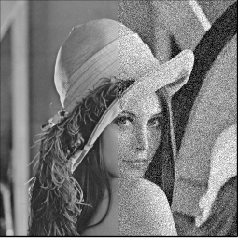
\includegraphics[width=0.4\textwidth]{graphics/lena_pic.jpg}\\
	\vspace{15pt}
	\small Image is partially destroyed\\
	\small Reconstruct image
}
\begin{frame}{Dictionary Learning: Basic Theory}
	\center Well-known machine learning model:
	\begin{equation*}
	\min_{D, \alpha} \frac{1}{N} \sum_{i=1}^N \|\underbrace{ x_i - D \alpha_i }_{\text{\alert{a) SQN}}}\|_2^2 + \underbrace{\lambda \| 
		\alpha_i \|_1}_{\text{\alert{b) Prox}}}
	\end{equation*}
	\center \alert{ 2-phase optimization problem}
	\begin{itemize}
		\item[1.] Update "dictionary" 
		\item[2.] Induce sparsity
	\end{itemize}
	$\Rightarrow$ Example: Reconstruction of partially distorted images
\end{frame}

\begin{frame}{Dictionary Learning in Image Reconstruction I}
	\begin{figure}[h!]
		\centering
		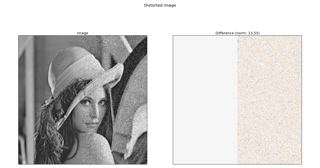
\includegraphics[width=0.8\textwidth]{graphics/lena_noisy.png}
		\caption{Noisy image}
	\end{figure}
\end{frame}

\begin{frame}{Dictionary Learning in Image Reconstruction II}
	\begin{figure}[h!]
		\centering
		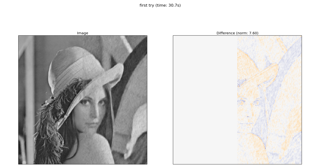
\includegraphics[width = 0.8\linewidth]{graphics/lena_reconstructed.png}
		\caption{Reconstructed image}
	\end{figure}
\end{frame}




\section{Conclusion}

  \begin{frame}{Summary}
    \begin{itemize}
    	\item Large amounts of data
    	\item Need for stochastic algorithms
    	\item Second order methods to improve speed
    	\item For smooth and non-smooth problems
    	\item Good performance of implementation on various problems
    \end{itemize}
    \phantom{\cite{SQN}\cite{becker2012quasi}\cite{mairal2010online}\cite{parikh2013proximal}}
  \end{frame}
\plain{
	
	
	\begin{center}
		
		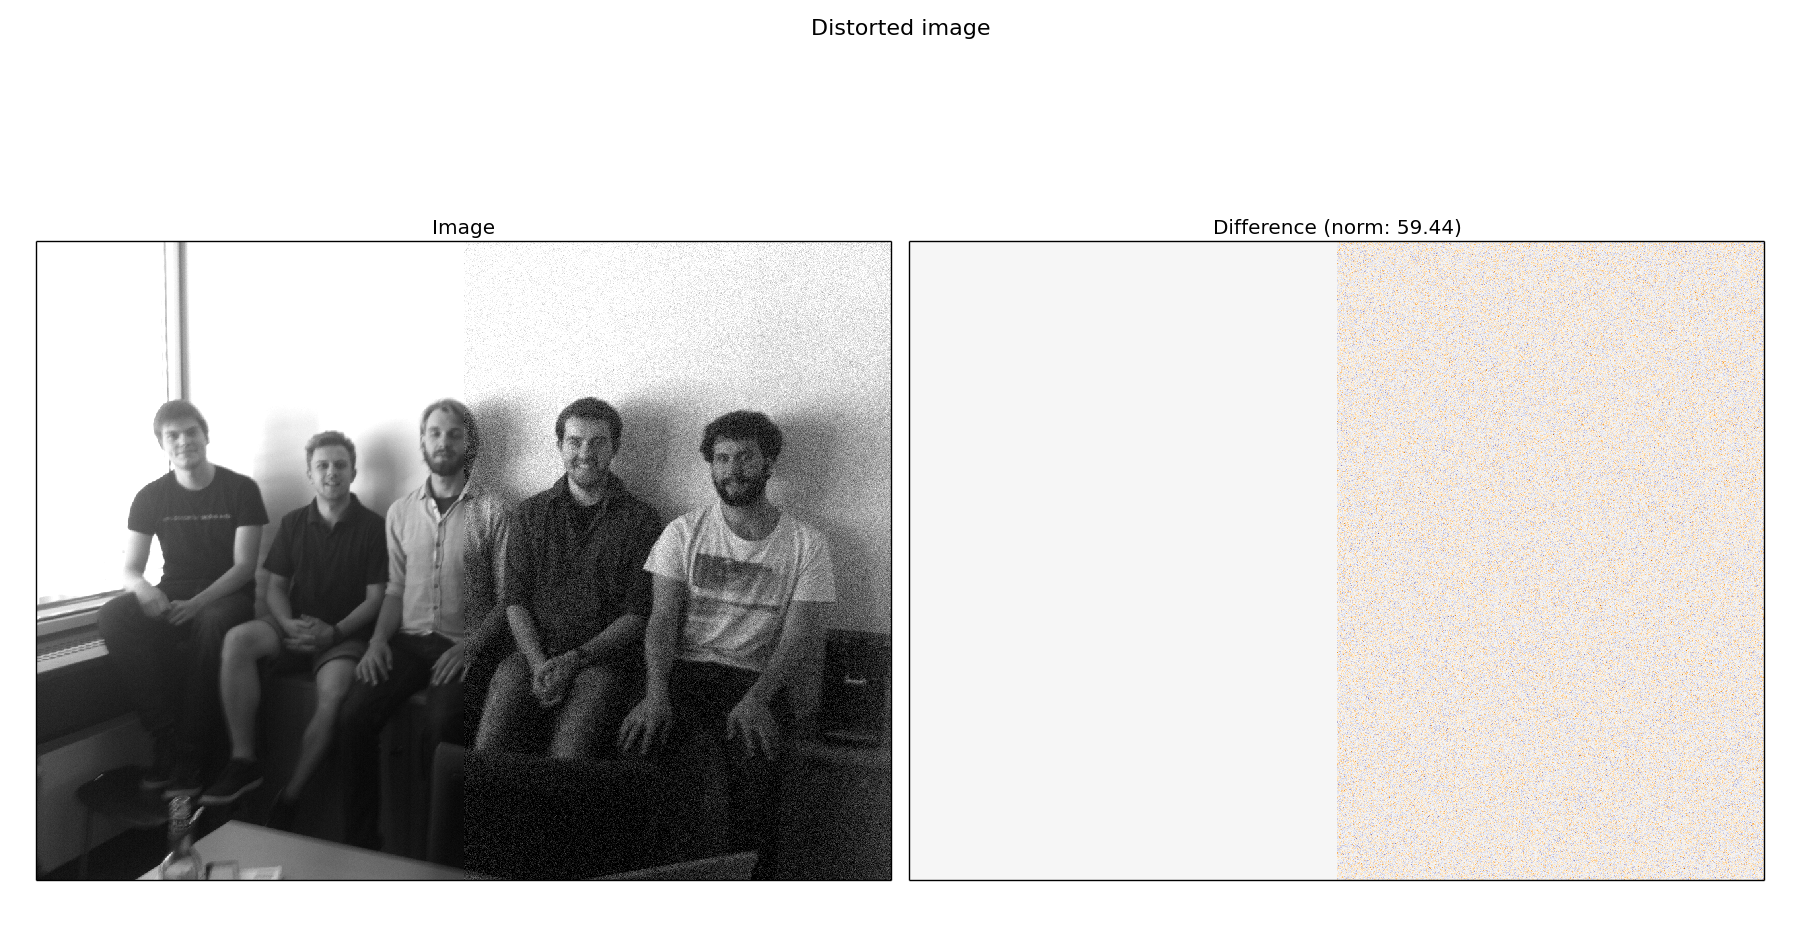
\includegraphics[width = 0.7\linewidth]{graphics/noisy_picture.png}\\
		
		
		
		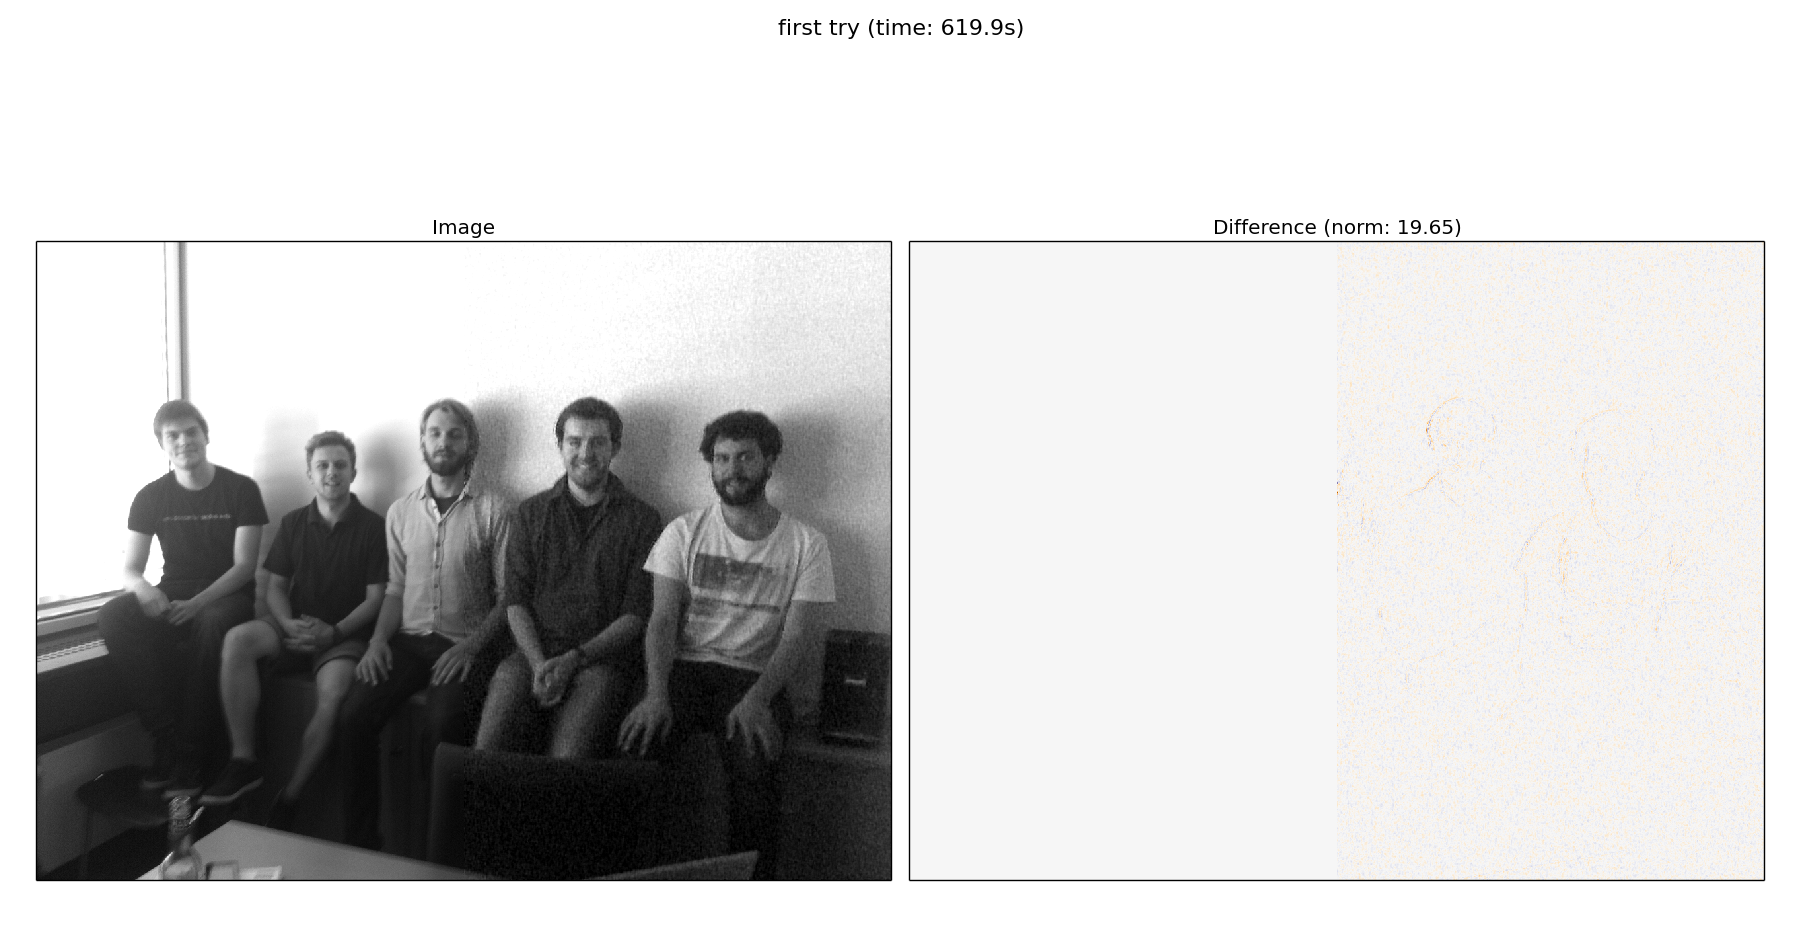
\includegraphics[width = 0.7\linewidth]{graphics/reconstructed.png}\\
	\end{center}
}  

  \plain{Questions?}

  \begin{frame}[allowframebreaks]


    {\footnotesize{
    \bibliographystyle{abbrv}
    \bibliography{refs}
    }
    }
    %\bibliography{refs}
    %\bibliographystyle{abbrv}

  \end{frame}



\end{document}
